\documentclass[11pt,oneside,a4paper]{report}

% 1. Course metadata and wording
\def\utprunninghead{Artificial Intelligence Notes}
\def\utplabtotal{8}
\def\utpcoursetitle{Artificial Intelligence}
\def\utpcourseoutline{Eight laboratory-guided modules covering search, fuzzy systems, robotics,\par natural language processing, and optimization, closing with game search.}
\def\utptitleintuition{Conceptual intuition}
\def\utptitlefirstread{Core material}
\def\utptitleoptional{Extension}
\def\utptitletryit{Practice}
\def\utptitlelabmode{Lab setup}
\def\utptitledeliverable{Submission checklist}

% 2. Shared presentation
% =====================================================================
%  utpnotes.tex
%  Shared preamble for the UTP teaching-assistant course notes.
%
%  Every book includes this file, and it is the ONLY file a book needs
%  from .shared/: the cover, the logos and the optional diagram
%  libraries are all reached from here. It owns everything the books
%  have in common, so a change here reaches every course at once.
%
%  ------------------------------------------------------------------
%  HOW A COURSE USES THIS FILE
%  ------------------------------------------------------------------
%      \documentclass[11pt,oneside,a4paper]{report}
%
%      \def\utprunninghead{Machine Learning Notes}   % section 1
%      \def\utplabtotal{8}
%      \def\utpcoursetitle{Machine Learning}
%      \def\utpcourseoutline{One or two lines for the cover.}
%
%      % =====================================================================
%  utpnotes.tex
%  Shared preamble for the UTP teaching-assistant course notes.
%
%  Every book includes this file, and it is the ONLY file a book needs
%  from .shared/: the cover, the logos and the optional diagram
%  libraries are all reached from here. It owns everything the books
%  have in common, so a change here reaches every course at once.
%
%  ------------------------------------------------------------------
%  HOW A COURSE USES THIS FILE
%  ------------------------------------------------------------------
%      \documentclass[11pt,oneside,a4paper]{report}
%
%      \def\utprunninghead{Machine Learning Notes}   % section 1
%      \def\utplabtotal{8}
%      \def\utpcoursetitle{Machine Learning}
%      \def\utpcourseoutline{One or two lines for the cover.}
%
%      % =====================================================================
%  utpnotes.tex
%  Shared preamble for the UTP teaching-assistant course notes.
%
%  Every book includes this file, and it is the ONLY file a book needs
%  from .shared/: the cover, the logos and the optional diagram
%  libraries are all reached from here. It owns everything the books
%  have in common, so a change here reaches every course at once.
%
%  ------------------------------------------------------------------
%  HOW A COURSE USES THIS FILE
%  ------------------------------------------------------------------
%      \documentclass[11pt,oneside,a4paper]{report}
%
%      \def\utprunninghead{Machine Learning Notes}   % section 1
%      \def\utplabtotal{8}
%      \def\utpcoursetitle{Machine Learning}
%      \def\utpcourseoutline{One or two lines for the cover.}
%
%      \input{../.shared/utpnotes}
%
%      \utpcontentspage{\small}{\normalsize}{0.65em}{0.07em}{0.16em}
%
%      \begin{document}
%      \utpfrontmatter                     % cover, contents, map
%      \part{Orientation}
%      \input{chapters/01-where-to-begin}
%      \end{document}
%
%  Configuration goes BEFORE the \input; overrides go AFTER it.
%  Paths are relative, so compile from inside the course folder.
%
%  ------------------------------------------------------------------
%  NAMING
%  ------------------------------------------------------------------
%  One name per idea, used by every book. Anything a book can use is
%  either an unprefixed learning box (keyidea, pitfall, labproject,
%  ...) or carries the utp prefix (utpfigure, utptable, utpfig,
%  utpsteps, utppython, UTPNavy, utpcell, ...). Course prefixes such
%  as ml-, ds- or erp- are not used: a chapter moved from one book to
%  another compiles unchanged. .shared/README.md lists every name.
%
%  Adding a new course? Copy .shared/TEMPLATE-main.tex and follow
%  .shared/ADDING-A-COURSE.md. Every step is a numbered checklist.
%
%  ------------------------------------------------------------------
%  CONTENTS
%  ------------------------------------------------------------------
%    1  Course configuration     the knobs a book may set
%    2  Packages                 the shared package set and fonts
%    3  Colour palette           the one UTP palette
%    4  Page layout and tables   margins, lists, table styling
%    5  Table of contents        parts, chapters, labs, figures
%    6  Headings                 chapter badge, part pages, sections
%    7  Page furniture           running heads and footers
%    8  Learning boxes           key idea, pitfall, try it, and friends
%    9  Small commands           \term, \cmd, \chapterguide, utpsteps
%   10  Diagram node styles      the TikZ vocabulary every book shares
%   11  Figure frames            utpfigure, utpfig, source images
%   12  Lab sheets               the lab banner and the lab toolkit
%   13  Stage divider            the part-opening page in longer books
%   14  Front matter             \utpfrontmatter: cover, contents, map
%   15  Listing styles           code, terminal and pseudocode
% =====================================================================

% --------------------------------------------------------------------
%  1.  COURSE CONFIGURATION
% --------------------------------------------------------------------
%  The knobs below, plus \utpstyleparts in section 5 and the box titles
%  in section 8, are the whole configuration surface. A book sets what
%  it needs BEFORE the \input and inherits the rest.
%
%  \providecommand means "define unless the book already did", which is
%  what makes the \def-before-\input pattern work.
%
%  Running text
%    \utprunninghead   the left running head on every page.
%    \utpchapterlabel  the word in the chapter badge. CHAPTER by
%                      default; a book whose chapters are labs sets LAB.
%    \utplabtotal      the N in the "Lab 3 of N" banners.

\providecommand{\utprunninghead}{Course Notes}
\providecommand{\utpchapterlabel}{CHAPTER}
\providecommand{\utplabtotal}{10}

%  Cover, printed by section 14
%    \utpcoursetitle       the title on the title page.
%    \utpdocumentsubtitle  the line under the title; Teaching Assistant Guide by default.
%    \utpcourseoutline     the sentence or two below it; \\ breaks a line.
%    \utpoutlineheading    the small heading above that sentence.
%    \utpauthor            the name in the PREPARED BY block.
%    \utpauthorrole        the line under the name.

\providecommand{\utpcoursetitle}{\utprunninghead}
\providecommand{\utpdocumentsubtitle}{Teaching Assistant Guide}
\providecommand{\utpcourseoutline}{}
\providecommand{\utpoutlineheading}{COURSE OUTLINE}
\providecommand{\utpauthor}{Reeyan Afzal Khan}
\providecommand{\utpauthorrole}{Graduate Research Assistant}

%  Files and folders
%    \utpextragraphicspath  image folders to search before the standard
%                           ones, as brace groups: {{screenshots/}}.
%                           A course's own figures/ folder and the
%                           shared logos are always searched.
%    \utpcoursemap          the overview chapter \utpfrontmatter inputs
%                           after the contents. Empty means none.

\providecommand{\utpextragraphicspath}{}
\providecommand{\utpcoursemap}{chapters/course-map}

%  Contents entries for chapters (section 5 applies them). A book whose
%  chapters are labs says so once here rather than restating the three
%  tocloft settings after the input.
%    \utpchaptertocword      Chapter~ by default, Lab~ in one book.
%    \utpchaptertocindent    left indent of the entry.
%    \utpchaptertocnumwidth  room reserved for the word and number.

\providecommand{\utpchaptertocword}{Chapter~}
\providecommand{\utpchaptertocindent}{1.5em}
\providecommand{\utpchaptertocnumwidth}{6em}

%  Monospace face (section 2)
%    \utpmonofont   sourcecodepro by default. inconsolata is the
%                   alternative, for a book whose pages are mostly
%                   device transcripts.

\providecommand{\utpmonofont}{sourcecodepro}

% --------------------------------------------------------------------
%  2.  PACKAGES
% --------------------------------------------------------------------
%  The union of what the books need. A course that needs something
%  extra loads it in its own file, under the heading "packages only
%  this book needs". Pseudocode is the one optional package the shared
%  file knows about: \utpusealgorithms in section 15 loads and styles it.
%
%  The tikz and pgfplots library lists are the union across all books,
%  so a diagram or chart copied from one course compiles in another.

\usepackage[T1]{fontenc}
\IfFileExists{glyphtounicode.tex}{\input{glyphtounicode}\pdfgentounicode=1}{}
\usepackage[american]{babel}
\IfFileExists{sourcesanspro.sty}
  {\usepackage[default]{sourcesanspro}}
  {\usepackage[scaled]{helvet}\renewcommand{\familydefault}{\sfdefault}}
\DeclareFontShape{T1}{cmss}{b}{n}{<->ssub*cmss/bx/n}{}
\DeclareFontShape{TS1}{cmss}{b}{n}{<->ssub*cmss/bx/n}{}
% Monospace. Without this the tt default stays Computer Modern Typewriter,
% a serif face that clashes with the sans body text in every listing and
% every \cmd. Source Code Pro is the companion to Source Sans Pro; it is
% scaled down because mono digits otherwise sit large next to the sans.
%
% Inconsolata, chosen with \def\utpmonofont{inconsolata}, distinguishes
% 0/O and 1/l/I at a glance, which matters when a reader copies an
% interface name or an address out of a transcript. Only one mono package
% is ever loaded: a second would win the family but inherit the first's
% series names, and every \ttfamily would then resolve by substitution.
\def\utpmonoinconsolata{inconsolata}
\ifx\utpmonofont\utpmonoinconsolata
  \IfFileExists{inconsolata.sty}{\usepackage[varqu,varl,scaled=1.02]{inconsolata}}{}
\else
  \IfFileExists{sourcecodepro.sty}
    {\usepackage[scaled=0.88]{sourcecodepro}}
    {\usepackage[scaled=0.86]{beramono}}
  % Source Sans names its normal weight "regular", but the Computer Modern
  % fallbacks call it "m". Map one onto the other so a \ttfamily reached
  % while the regular series is active resolves instead of warning.
  \DeclareFontShape{T1}{cmtt}{regular}{n}{<->ssub*cmtt/m/n}{}
  \DeclareFontShape{TS1}{cmtt}{regular}{n}{<->ssub*cmtt/m/n}{}
  \DeclareFontShape{T1}{cmtt}{regular}{it}{<->ssub*cmtt/m/it}{}
\fi
\usepackage[margin=21mm,headheight=22pt]{geometry}
\usepackage{amsmath,amssymb,mathtools,bm}
\usepackage{microtype}
\usepackage{enumitem}
\usepackage{booktabs}
\usepackage{tabularx}
\usepackage{array}
\usepackage{ragged2e}
\usepackage{etoolbox}
\usepackage{titlesec}
\usepackage{tocloft}
\usepackage{fancyhdr}
\usepackage[table]{xcolor}
\usepackage{tcolorbox}
\tcbuselibrary{breakable,skins}
\usepackage[hidelinks]{hyperref}
\usepackage{bookmark}
% Document properties, so the PDF identifies itself in a reader's
% title bar, in a library catalogue, and in search results. Set from
% the same configuration macros the cover uses.
\hypersetup{
  pdftitle={\utpcoursetitle},
  pdfauthor={\utpauthor},
  pdfsubject={Universiti Teknologi PETRONAS course notes and laboratory guide},
  pdfkeywords={UTP, course notes, laboratory manual, \utpcoursetitle},
  pdfdisplaydoctitle=true,
  bookmarksnumbered=true,
  bookmarksopenlevel=1
}
\usepackage{listings}
\usepackage{graphicx}
\usepackage{caption}
\usepackage{tikz}
\usetikzlibrary{angles,arrows.meta,backgrounds,calc,chains,decorations.pathmorphing,decorations.pathreplacing,fit,matrix,patterns,positioning,quotes,shadows.blur,shapes.geometric,shapes.misc,shapes.symbols}
\usepackage{pgfplots}
% statistics gives boxplot prepared; groupplots gives multi-panel charts.
\usepgfplotslibrary{statistics}
\usepgfplotslibrary{groupplots}

% Images: any folders the book names first, then its own figures/
% folder, then the shared logos used by the cover.
\expandafter\graphicspath\expandafter{\utpextragraphicspath{figures/}{../.shared/logos/}}

% --------------------------------------------------------------------
%  3.  COLOUR PALETTE
% --------------------------------------------------------------------
%  One palette, defined once under UTP* names, and used by every book,
%  box, diagram and chart. Five accents (blue, teal, green, orange, red)
%  with a pale tint of each for box backgrounds, plus navy for headings,
%  gold for the cover, ink and muted for text, and a sixth accent,
%  purple, for charts and layered diagrams that need one more series.

\definecolor{UTPNavy}{HTML}{18324A}
\definecolor{UTPBlue}{HTML}{246B9E}
\definecolor{UTPTeal}{HTML}{138A80}
\definecolor{UTPGreen}{HTML}{2D7D46}
\definecolor{UTPOrange}{HTML}{C86B24}
\definecolor{UTPRed}{HTML}{B34843}
\definecolor{UTPPurple}{HTML}{6B4FA0}
\definecolor{UTPGold}{HTML}{D4A13E}
\definecolor{UTPInk}{HTML}{263238}
\definecolor{UTPMuted}{HTML}{60717C}
\definecolor{UTPPaleBlue}{HTML}{EEF6FB}
\definecolor{UTPPaleTeal}{HTML}{EEF8F6}
\definecolor{UTPPaleOrange}{HTML}{FFF5EA}
\definecolor{UTPPaleRed}{HTML}{FFF0EF}
\definecolor{UTPPalePurple}{HTML}{F0ECF9}
\definecolor{UTPPaleGray}{HTML}{F4F6F7}
\color{UTPInk}

% --------------------------------------------------------------------
%  4.  PAGE LAYOUT AND TABLES
% --------------------------------------------------------------------
%  Paragraph spacing, list indents, and the table look: alternating
%  row tint, top-aligned paragraph columns, ragged-right cells.
%
%  Two extra column types for tabularx tables:
%      D{width}   a fixed-width, ragged-right, vertically centred column
%      Y          a ragged-right column that fills the remaining width
%
%  Every table in every book has the same shape, the one Algorithms &
%  Data Structures set: a utptable frame around a full-width tabularx,
%  booktabs rules, a tinted header row of \utpth cells (centred, bold,
%  navy), and a first column in bold navy when it names the rows.
%  Cells are vertically centred, so use m{} rather than p{} columns.
%
%      \begin{utptable}
%      \begin{tabularx}{\linewidth}{@{}>{\bfseries\leavevmode\color{UTPNavy}}m{0.22\linewidth}X@{}}
%      \toprule
%      \rowcolor{UTPPaleBlue!92}
%      \utpth{Operation} & \utpth{What it does} \\
%      \midrule
%      Insertion & Add a new element. \\
%      \bottomrule
%      \end{tabularx}
%      \end{utptable}
%
%  A book whose tables carry dense text asks for \utpcompacttables after
%  the input: tabularx tables then set in \footnotesize with tighter
%  padding and vertically centred cells.

\setlength{\parindent}{0pt}
\setlength{\parskip}{0.55em}
\setlist[itemize]{leftmargin=1.45em,itemsep=0.22em,topsep=0.25em}
\setlist[enumerate]{leftmargin=1.75em,itemsep=0.28em,topsep=0.3em}
\setlist[description]{font=\bfseries\color{UTPNavy},itemsep=0.25em,topsep=0.3em}
\renewcommand{\arraystretch}{1.34}
\setlength{\tabcolsep}{6.5pt}
\arrayrulecolor{UTPBlue!45}
% Keep paragraph-style columns ragged and vertically centred. Tables use
% fixed m columns beside flexible X columns; giving X the same centring
% keeps a short cell level with a tall neighbour in a multi-line row.
\renewcommand{\tabularxcolumn}[1]{m{#1}}
\makeatletter
\g@addto@macro\@arrayparboxrestore{\RaggedRight\arraybackslash}
\makeatother
% A header cell: centred, bold and navy, on the tinted header row.
\newcommand{\utpth}[1]{\multicolumn{1}{c}{\bfseries\color{UTPNavy}#1}}
\AtBeginEnvironment{tabular}{\small\setlength{\extrarowheight}{0.6pt}\rowcolors{2}{UTPPaleBlue!72}{white}}
\AtBeginEnvironment{tabularx}{\small\setlength{\extrarowheight}{0.6pt}\rowcolors{2}{UTPPaleBlue!72}{white}}
\AtBeginEnvironment{figure}{\centering}
\newcolumntype{D}[1]{>{\raggedright\arraybackslash}m{#1}}
\newcolumntype{Y}{>{\raggedright\arraybackslash}X}
\newcommand{\utpcompacttables}{%
  \renewcommand{\tabularxcolumn}[1]{m{##1}}%
  \AtBeginEnvironment{tabularx}{%
    \footnotesize
    \setlength{\tabcolsep}{4pt}%
    \renewcommand{\arraystretch}{1.25}%
    \setlength{\extrarowheight}{0.6pt}%
  }%
}
\emergencystretch=1.5em
\hbadness=10000
\hfuzz=8pt

% Page-breaking discipline. Without these a paragraph can leave a single
% line stranded at the foot of one page or the head of the next, which is
% the most visible sign of unattended typesetting.
\widowpenalty=10000          % no first line of a paragraph left alone at a page foot
\clubpenalty=10000           % no last line of a paragraph left alone at a page head
\displaywidowpenalty=10000   % the same around displayed equations
\brokenpenalty=10000         % do not break a page after a hyphenated line
\predisplaypenalty=10000     % keep the line before a display with it
% Pages are built from boxes of many heights, so let the last line float
% up rather than stretching the gaps between boxes to force a flush foot.
\raggedbottom
% Prefer a slightly loose line to an overfull one, but do not hyphenate
% freely -- short sans lines look ragged when over-hyphenated.
\tolerance=1200
\hyphenpenalty=200

% Character protrusion and font expansion. Both are what stop a justified
% sans column from showing visible rivers down the page.
\microtypesetup{protrusion=true,expansion=true,tracking=true}

\pgfplotsset{
  compat=1.18,
  every axis/.append style={
    axis line style={draw=UTPMuted!85,line width=0.55pt},
    tick style={draw=UTPMuted!85},
    tick label style={font=\scriptsize\color{UTPMuted}},
    label style={font=\small\color{UTPNavy}},
    title style={font=\small\bfseries\color{UTPNavy}},
    legend style={font=\scriptsize,draw=UTPBlue!22,fill=white,rounded corners=1pt}
  },
  every axis plot/.append style={line width=1.15pt}
}
\tikzset{every picture/.append style={line cap=round,line join=round}}

% --------------------------------------------------------------------
%  5.  TABLE OF CONTENTS
% --------------------------------------------------------------------
%  Formatting for part, chapter and lab entries, and for a list of
%  figures if a book prints one. The lab level is a custom tocloft list
%  so lab banners appear in the contents.
%
%  Part styling is skipped when \utpstyleparts is 0, which is what a
%  book without \part divisions should set.
%
%  The contents page is meant to fill exactly one page, and how loosely
%  it is set depends on how many entries a book has. One line after the
%  input tunes it:
%
%      \utpcontentspage{<base size>}{<part size>}%
%                      {<space before a part>}{<before a chapter>}{<before a lab>}
%      \utpcontentspage{\normalsize}{\large}{1.15em}{0.38em}{0.30em}   % the default

\addto\captionsamerican{\renewcommand{\contentsname}{Learning Path}}
\newlistentry{lab}{toc}{-1}
\providecommand{\utpstyleparts}{1}
\ifnum\utpstyleparts=1
\renewcommand{\cftpartpresnum}{}
\renewcommand{\cftpartaftersnum}{}
\setlength{\cftpartnumwidth}{5.2em}
\setlength{\cftbeforepartskip}{0.38em}
\renewcommand{\cftpartfont}{\normalsize\bfseries\color{UTPNavy}}
\renewcommand{\cftpartpagefont}{\normalsize\bfseries\color{UTPNavy}}
\renewcommand{\cftpartleader}{\hfill}
\fi
\renewcommand{\cftchappresnum}{\utpchaptertocword}
\renewcommand{\cftchapaftersnum}{\quad}
\setlength{\cftchapindent}{\utpchaptertocindent}
\setlength{\cftchapnumwidth}{\utpchaptertocnumwidth}
\setlength{\cftbeforechapskip}{0pt}
\renewcommand{\cftchapfont}{\normalfont}
\renewcommand{\cftchappagefont}{\normalfont}
\renewcommand{\cftchapleader}{\cftdotfill{\cftdotsep}}
\setlength{\cftlabindent}{3em}
\setlength{\cftlabnumwidth}{0em}
\setlength{\cftbeforelabskip}{0.10em}
\renewcommand{\cftlabfont}{\bfseries\color{UTPOrange!90!black}}
\renewcommand{\cftlabpagefont}{\bfseries\color{UTPOrange!90!black}}
\renewcommand{\cftlableader}{\color{UTPOrange!65!UTPMuted}\cftdotfill{\cftlabdotsep}}

% A list of figures, for a book that prints one (\listoffigures).
\renewcommand{\cftfigfont}{\normalfont\small}
\renewcommand{\cftfigpagefont}{\normalfont\small}
\renewcommand{\cftfigpresnum}{Figure~}
\renewcommand{\cftfigaftersnum}{\quad}
\setlength{\cftfigindent}{1.5em}
\setlength{\cftfignumwidth}{5.6em}
\setlength{\cftbeforefigskip}{0pt}
\renewcommand{\cftfigleader}{\cftdotfill{\cftdotsep}}

% The contents page itself, printed by \utpfrontmatter (section 14).
\newcommand{\utpcontentspage}[5]{%
  \def\utptocsize{#1}\def\utptocpartsize{#2}%
  \def\utptocpartskip{#3}\def\utptocchapterskip{#4}\def\utptoclabskip{#5}}
\utpcontentspage{\normalsize}{\large}{1.15em}{0.38em}{0.30em}
\newcommand{\utptableofcontents}{%
  \begingroup
  \utptocsize
  \setlength{\parskip}{0pt}%
  \setlength{\cftbeforepartskip}{\utptocpartskip}%
  \setlength{\cftbeforechapskip}{\utptocchapterskip}%
  \setlength{\cftbeforelabskip}{\utptoclabskip}%
  \renewcommand{\cftpartfont}{\utptocpartsize\bfseries\color{UTPNavy}}%
  \renewcommand{\cftpartpagefont}{\utptocpartsize\bfseries\color{UTPNavy}}%
  \tableofcontents
  \endgroup
}

% --------------------------------------------------------------------
%  6.  HEADINGS
% --------------------------------------------------------------------
%  The chapter badge (a coloured block with a word and the number),
%  part pages, and section spacing.
%
%  The word in the badge is \utpchapterlabel; Data Communication sets
%  it to LAB because each of its chapters is a lab.

\titleformat{\chapter}[display]
  {\bfseries\color{UTPNavy}}
  {\filleft\colorbox{UTPBlue}{\parbox{2.55cm}{\centering\color{white}\Large
    \utpchapterlabel\\[-0.15em]\Huge\thechapter}}}
  {0.65em}{\Huge\raggedright}
  [\vspace{0.25em}{\color{UTPBlue}\titlerule[1.2pt]}]
\renewcommand{\thepart}{Stage~\arabic{part}}
\titleformat{\part}[display]
  {\centering\color{UTPNavy}\bfseries}
  {\Large\color{UTPTeal}\thepart}{0.45em}{\Huge}
  [\vspace{0.55em}\color{UTPTeal}\rule{0.45\linewidth}{1.5pt}]
\titleformat{\section}{\Large\bfseries\color{UTPNavy}}{\thesection}{0.55em}{}
\titleformat{\subsection}{\large\bfseries\color{UTPBlue}}{\thesubsection}{0.5em}{}
\titlespacing*{\chapter}{0pt}{-1.8em}{1.0em}
\titlespacing*{\part}{0pt}{0pt}{1em}
\titlespacing*{\section}{0pt}{1.2em}{0.35em}
\titlespacing*{\subsection}{0pt}{0.95em}{0.2em}

% --------------------------------------------------------------------
%  7.  PAGE FURNITURE
% --------------------------------------------------------------------
%  Running heads and footers. The left header is \utprunninghead;
%  the right one follows the current chapter.

\pagestyle{fancy}
\fancyhf{}
\lhead{\small\color{UTPMuted}\utprunninghead}
\rhead{\small\color{UTPMuted}\nouppercase{\leftmark}}
\cfoot{\small\color{UTPMuted}\thepage}
\renewcommand{\headrulewidth}{0.5pt}
\renewcommand{\headrule}{\hbox to\headwidth{\color{UTPPaleBlue}\leaders\hrule height \headrulewidth\hfill}}
\renewcommand{\chaptermark}[1]{\markboth{#1}{}}
\fancypagestyle{plain}{%
  \fancyhf{}%
  \cfoot{\small\color{UTPMuted}\thepage}%
  \renewcommand{\headrulewidth}{0pt}%
}

% --------------------------------------------------------------------
%  8.  LEARNING BOXES
% --------------------------------------------------------------------
%  The coloured callouts the chapters use. Every title is a macro, so
%  a book can rename a box without restating its geometry:
%
%      \def\utptitlepitfall{Technical note}   % before the input
%
%  To change how a box LOOKS in one book, use one of the named
%  variations at the end of this section, or \renewtcolorbox after the
%  input. To add a box only one book needs, declare it in that book
%  with \utpnewcallout or \utpnewquietbox.

% Box titles -- override any of these before the input line.
\providecommand{\utptitlekeyidea}{Key idea}
\providecommand{\utptitleworked}{Worked example}
\providecommand{\utptitlepitfall}{Common mistake}
\providecommand{\utptitletryit}{Try it yourself}
\providecommand{\utptitlequickcheck}{Check your understanding}
\providecommand{\utptitlerecap}{Chapter recap}
\providecommand{\utptitledeliverable}{Lab deliverable}
\providecommand{\utptitlelabmode}{How much is scaffolded?}
\providecommand{\utptitleintuition}{Plain idea}
\providecommand{\utptitlefirstread}{Core path}
\providecommand{\utptitleglance}{Chapter at a glance}
\providecommand{\utptitledebug}{Debugging task}
\providecommand{\utptitleoptional}{Beyond the core}
\providecommand{\utptitleverification}{Verification checklist}
\providecommand{\utptitletroubleshoot}{Troubleshooting}
\providecommand{\utptitlesourcebasis}{Source basis}

% Explaining an idea
\newtcolorbox{keyidea}{enhanced,breakable,colback=UTPPaleTeal,colframe=UTPTeal, boxrule=0.8pt,arc=2mm,left=2.5mm,right=2.5mm,top=1.8mm,bottom=1.8mm, fonttitle=\bfseries\color{UTPNavy},title=\utptitlekeyidea}
\newtcolorbox{workedexample}{enhanced,breakable,colback=UTPPaleBlue,colframe=UTPBlue, boxrule=0.8pt,arc=2mm,left=2.5mm,right=2.5mm,top=1.8mm,bottom=1.8mm, fonttitle=\bfseries\color{UTPNavy},title=\utptitleworked}
\newtcolorbox{pitfall}{enhanced,breakable,colback=UTPPaleRed,colframe=UTPRed, boxrule=0.8pt,arc=2mm,left=2.5mm,right=2.5mm,top=1.8mm,bottom=1.8mm, fonttitle=\bfseries\color{UTPNavy},title=\utptitlepitfall}
% Asking the reader to do something
\newtcolorbox{tryit}{enhanced,breakable,colback=white,colframe=UTPTeal, boxrule=0.9pt,arc=2mm,left=2.5mm,right=2.5mm,top=1.8mm,bottom=1.8mm, fonttitle=\bfseries\color{white},colbacktitle=UTPTeal,title=\utptitletryit}
\newtcolorbox{quickcheck}{enhanced,breakable,colback=white,colframe=UTPOrange, boxrule=0.9pt,arc=2mm,left=2.5mm,right=2.5mm,top=1.8mm,bottom=1.8mm, fonttitle=\bfseries\color{white},colbacktitle=UTPOrange,title=\utptitlequickcheck}
\newtcolorbox{chapterrecap}{enhanced,breakable,colback=UTPPaleTeal,colframe=UTPGreen, boxrule=0.9pt,arc=2mm,left=2.5mm,right=2.5mm,top=1.8mm,bottom=1.8mm, fonttitle=\bfseries\color{white},colbacktitle=UTPGreen,title=\utptitlerecap}
% Lab structure
\newtcolorbox{labdeliverable}{enhanced,breakable,colback=white,colframe=UTPGreen, boxrule=0.9pt,arc=2mm,left=2.6mm,right=2.6mm,top=1.9mm,bottom=1.9mm, fonttitle=\bfseries\color{white},colbacktitle=UTPGreen,title=\utptitledeliverable}
\newtcolorbox{labmode}{enhanced,breakable,colback=UTPPaleBlue!52,colframe=UTPBlue, boxrule=0.75pt,arc=2mm,left=2.6mm,right=2.6mm,top=1.7mm,bottom=1.7mm, fonttitle=\bfseries\color{white},colbacktitle=UTPBlue,title=\utptitlelabmode}
% Softer, lighter-weight asides
\newtcolorbox{intuition}{enhanced,breakable,colback=white,colframe=UTPOrange!42, boxrule=0.5pt,arc=2mm,left=2.5mm,right=2.5mm,top=1.5mm,bottom=1.5mm, fonttitle=\bfseries\color{UTPOrange!85!black},title=\utptitleintuition}
\newtcolorbox{firstread}{enhanced,breakable,colback=white,colframe=UTPBlue!42, boxrule=0.5pt,arc=2mm,left=2.5mm,right=2.5mm,top=1.5mm,bottom=1.5mm, fonttitle=\bfseries\color{UTPBlue}, title=\utptitlefirstread}
\newtcolorbox{debugtask}{enhanced,breakable,colback=UTPPaleRed!58,colframe=UTPRed, boxrule=0.85pt,arc=2mm,left=2.6mm,right=2.6mm,top=1.9mm,bottom=1.9mm, fonttitle=\bfseries\color{white},colbacktitle=UTPRed,title=\utptitledebug}
\newtcolorbox{analogy}{enhanced,breakable,colback=white,colframe=UTPOrange!38, boxrule=0.5pt,arc=2mm,left=2.5mm,right=2.5mm,top=1.5mm,bottom=1.5mm, fonttitle=\bfseries\color{UTPOrange!85!black},title=Analogy}
\newtcolorbox{coursechoice}{enhanced,breakable,colback=white,colframe=UTPNavy, boxrule=0.8pt,arc=2mm,left=2.8mm,right=2.8mm,top=2mm,bottom=2mm, fonttitle=\bfseries\color{white},colbacktitle=UTPNavy,title=Course choice}
\newtcolorbox{decisionmemo}{enhanced,breakable,colback=UTPPaleOrange!55,colframe=UTPOrange, boxrule=0.85pt,arc=2mm,left=2.6mm,right=2.6mm,top=1.9mm,bottom=1.9mm, fonttitle=\bfseries\color{white},colbacktitle=UTPOrange,title=Decision memo}
\newtcolorbox{libnote}{enhanced,breakable,colback=white,colframe=UTPMuted!48, boxrule=0.5pt,arc=2mm,left=2.5mm,right=2.5mm,top=1.5mm,bottom=1.5mm, fonttitle=\bfseries\color{UTPNavy},title=Reference note}
\newtcolorbox{miniproject}{enhanced,breakable,colback=UTPPaleTeal!52,colframe=UTPGreen, boxrule=0.9pt,arc=2mm,left=2.6mm,right=2.6mm,top=1.9mm,bottom=1.9mm, fonttitle=\bfseries\color{white},colbacktitle=UTPGreen,title=Mini-project}
% Where the material came from: the lecturer's slides, manual or tutorial
% that a chapter is built on.
\newtcolorbox{sourcebasis}{enhanced,breakable,colback=white,colframe=UTPMuted!55, boxrule=0.5pt,arc=2mm,left=2.5mm,right=2.5mm,top=1.5mm,bottom=1.5mm, fonttitle=\bfseries\color{UTPMuted},title=\utptitlesourcebasis}
% Boxes that take a title argument
\newtcolorbox{modelcard}[1]{enhanced,breakable,colback=white,colframe=UTPBlue, boxrule=0.9pt,arc=2mm,left=2.5mm,right=2.5mm,top=1.8mm,bottom=1.8mm, fonttitle=\bfseries\color{white},colbacktitle=UTPBlue,title=#1}
\newtcolorbox{optionaltopic}{enhanced,breakable,colback=white,colframe=UTPMuted!58, boxrule=0.5pt,arc=2mm,left=2.5mm,right=2.5mm,top=1.5mm,bottom=1.5mm, fonttitle=\bfseries\color{UTPMuted},title=\utptitleoptional}
\newtcolorbox{secondpass}{enhanced,breakable,colback=UTPPaleGray!82,colframe=UTPMuted, boxrule=0.75pt,arc=2mm,left=2.6mm,right=2.6mm,top=1.9mm,bottom=1.9mm, fonttitle=\bfseries\color{white},colbacktitle=UTPMuted,title=Second pass}
\newtcolorbox{labproject}[1]{enhanced,breakable,colback=white,colframe=UTPBlue, boxrule=0.9pt,arc=2mm,left=2.6mm,right=2.6mm,top=1.9mm,bottom=1.9mm, fonttitle=\bfseries\color{white},colbacktitle=UTPBlue,title={#1}}
% Evidence that a lab worked, and what to do when it did not
\newtcolorbox{verification}{enhanced,breakable,colback=UTPPaleTeal!65,colframe=UTPGreen, boxrule=0.8pt,arc=2mm,left=2.6mm,right=2.6mm,top=1.8mm,bottom=1.8mm, fonttitle=\bfseries\color{white},colbacktitle=UTPGreen,title=\utptitleverification}
\newtcolorbox{troubleshoot}{enhanced,breakable,colback=UTPPaleOrange!70,colframe=UTPOrange, boxrule=0.8pt,arc=2mm,left=2.6mm,right=2.6mm,top=1.8mm,bottom=1.8mm, fonttitle=\bfseries\color{white},colbacktitle=UTPOrange,title=\utptitletroubleshoot}

% Named variations a book asks for after the input. Each restyles boxes
% that already exist, so the chapters do not change.
%
%   \utpheavycallouts          a solid colour bar behind the titles of
%                              keyidea, workedexample, intuition and
%                              firstread, with a firmer frame.
%   \utpbreakableframes        let utpfigure and utptable split over a
%                              page break, in a lighter blue (section 11).
%   \utplabprojectcolour{...}  the labproject box in another colour, with
%                              a little more room inside.
\newcommand{\utplabprojectcolour}[1]{%
  \renewtcolorbox{labproject}[1]{enhanced,breakable,colback=white,colframe=#1, boxrule=0.9pt,arc=2mm,left=2.7mm,right=2.7mm,top=2mm,bottom=2mm, fonttitle=\bfseries\color{white},colbacktitle=#1,title={##1}}%
}
\newcommand{\utpheavycallouts}{%
  \renewtcolorbox{keyidea}{enhanced,breakable,colback=UTPPaleTeal,colframe=UTPTeal, boxrule=0.85pt,arc=2mm,left=2.5mm,right=2.5mm,top=1.8mm,bottom=1.8mm, fonttitle=\bfseries\color{white},colbacktitle=UTPTeal,title=\utptitlekeyidea}%
  \renewtcolorbox{workedexample}{enhanced,breakable,colback=UTPPaleBlue,colframe=UTPBlue, boxrule=0.8pt,arc=2mm,left=2.5mm,right=2.5mm,top=1.8mm,bottom=1.8mm, fonttitle=\bfseries\color{white},colbacktitle=UTPBlue,title=\utptitleworked}%
  \renewtcolorbox{intuition}{enhanced,breakable,colback=UTPPaleOrange,colframe=UTPOrange, boxrule=0.8pt,arc=2mm,left=2.5mm,right=2.5mm,top=1.8mm,bottom=1.8mm, fonttitle=\bfseries\color{white},colbacktitle=UTPOrange,title=\utptitleintuition}%
  \renewtcolorbox{firstread}{enhanced,breakable,colback=white,colframe=UTPBlue, boxrule=0.9pt,arc=2mm,left=2.5mm,right=2.5mm,top=1.8mm,bottom=1.8mm, fonttitle=\bfseries\color{white},colbacktitle=UTPBlue,title=\utptitlefirstread}%
}

% Declaring a box a single book needs. Both constructors take the house
% geometry and let a trailing key list override any of it, so a new box
% is one line and still matches the others:
%
%   \utpnewcallout{odoobox}{white}{UTPBlue}{Odoo 19 Community}
%   \utpnewcallout[boxrule=0.9pt]{name}{back}{frame}{Title}
%   \utpnewquietbox{referencebox}{UTPMuted!58}{UTPMuted}{Reference note}
%
% A callout is a tinted box under a solid title bar, for something the
% reader has to act on. A quiet box is a light frame with coloured
% title text, for an aside they can read past. If a second book ever
% wants the same box, move its line into this section.
\newcommand{\utpnewcallout}[5][]{%
  \newtcolorbox{#2}{enhanced,breakable,colback=#3,colframe=#4, boxrule=0.8pt,arc=2mm,left=2.6mm,right=2.6mm,top=1.8mm,bottom=1.8mm, fonttitle=\bfseries\color{white},colbacktitle=#4,title={#5},#1}%
}
\newcommand{\utpnewquietbox}[5][]{%
  \newtcolorbox{#2}{enhanced,breakable,colback=white,colframe=#3, boxrule=0.5pt,arc=2mm,left=2.5mm,right=2.5mm,top=1.5mm,bottom=1.5mm, fonttitle=\bfseries\color{#4},title={#5},#1}%
}

% --------------------------------------------------------------------
%  9.  SMALL COMMANDS
% --------------------------------------------------------------------
%  \term for a defined term, \cmd for inline code, \chapref and
%  \secref for cross-references, and the utpsteps numbered-step list.
%
%      \term{overfitting}          a term being defined
%      \cmd{git status}            inline code, in any language
%      \chapref{ch:trees}          "Chapter 12"
%      \secref{sec:pruning}        "Section 12.3"
%      \chapterguide{prior}{outcomes}   the box that opens a chapter
%      \begin{utpsteps} ... \end{utpsteps}  a numbered Step 1/Step 2 list
%
%  The second group is the shorthand the chapters use in running text:
%
%      \figref{fig:tree}           "Figure 4.2"
%      \chapsref{ch:a}{ch:b}       "Chapters 3--5"
%      \lib{pandas}                a library name
%      \cxg{x}, \cxo{x}, \cxr{x}   maths coloured green/orange/red
%      \given                      the bar in P(a \given b)
%      \coretag, \latertag         read-now / come-back-to markers
%      \kagglesource{url}{name}    the dataset a lab is built on

\newcommand{\term}[1]{\textbf{\color{UTPNavy}#1}}
\newcommand{\cmd}[1]{\texttt{#1}}
\newcommand{\chapref}[1]{Chapter~\ref{#1}}
\newcommand{\secref}[1]{Section~\ref{#1}}
\newcommand{\chapterguide}[2]{%
  \begin{tcolorbox}[enhanced,breakable,colback=white,colframe=UTPNavy,boxrule=0.8pt,
    arc=2mm,left=2.5mm,right=2.5mm,top=2mm,bottom=2mm,
    title=\utptitleglance,fonttitle=\bfseries\color{white},colbacktitle=UTPNavy]
    \textbf{Before you start:} #1\par
    \textbf{By the end, you can:} #2
  \end{tcolorbox}}
\newenvironment{utpsteps}
  {\begin{enumerate}[label=\textcolor{UTPBlue}{\bfseries Step~\arabic*:},leftmargin=4.5em,itemsep=0.38em]}
  {\end{enumerate}}

\newcommand{\figref}[1]{Figure~\ref{#1}}
\newcommand{\chapsref}[2]{Chapters~\ref{#1}--\ref{#2}}
\newcommand{\lib}[1]{\textbf{\color{UTPBlue}\texttt{#1}}}
\newcommand{\cxg}[1]{{\color{UTPGreen}\bfseries $#1$}}
\newcommand{\cxo}[1]{{\color{UTPOrange}\bfseries $#1$}}
\newcommand{\cxr}[1]{{\color{UTPRed}\bfseries $#1$}}
\newcommand{\given}{\mathrel{|}}
\DeclareMathOperator*{\argmin}{arg\,min}
\DeclareMathOperator*{\argmax}{arg\,max}
\newcommand{\coretag}{\par\smallskip\noindent\colorbox{UTPPaleBlue}{\strut\small\bfseries\color{UTPBlue}CORE NOW}\par\smallskip}
\newcommand{\latertag}{\par\smallskip\noindent\colorbox{UTPPaleGray}{\strut\small\bfseries\color{UTPMuted}RETURN LATER}\par\smallskip}
\newcommand{\kagglesource}[2]{%
  \par\smallskip\noindent\textbf{Kaggle source:} \href{#1}{#2}\par
}

% --------------------------------------------------------------------
%  10.  DIAGRAM NODE STYLES
% --------------------------------------------------------------------
%  The vocabulary the hand-drawn TikZ diagrams are built from: a cell
%  in an array, the one cell under the cursor, a circular graph node,
%  the arrow between two of them. Every book has the whole set:
%
%      utpcell, utphot, utpdone, utpdim, utpwall        array cells
%      utpnode, utpnodehot, utpnodedone, utpnodedim     graph nodes
%      utparrow, utpptr, utpdash, utpedge               connectors
%      utplabel, utptag, utpbrace                       annotation
%      utpstep, utpstage, utppanel, utpbox              boxes
%
%  A cell is 1.0cm by 0.8cm. A book whose diagrams were drawn to a
%  different grid resizes the cells once, after the input:
%
%      \utpdiagramsize{1.05cm}{0.85cm}
%
%  Larger vocabularies for one kind of drawing live in .shared/diagrams/
%  and are loaded by name, after the input:
%
%      \utpusediagrams{network}         devices, links, packet headers,
%                                       sequence diagrams, state machines
%      \utpusediagrams{process}         business-process flows, documents,
%                                       swimlanes, status chips
%      \utpusediagrams{data-objects}    vectors, lists and data frames
%                                       drawn as cells; flowcharts
%      \utpusediagrams{network,process} several at once

\newcommand{\utpdiagramsize}[2]{%
  \tikzset{
    utpcell/.style={draw=UTPBlue,fill=UTPPaleBlue,minimum width=#1,minimum height=#2,
                    font=\small\bfseries\color{UTPNavy},inner sep=1pt},
    utphot/.style={draw=UTPOrange,fill=UTPPaleOrange,minimum width=#1,minimum height=#2,
                   font=\small\bfseries\color{UTPNavy},line width=1pt,inner sep=1pt},
    utpdone/.style={draw=UTPGreen,fill=UTPPaleTeal,minimum width=#1,minimum height=#2,
                    font=\small\bfseries\color{UTPNavy},inner sep=1pt},
    utpdim/.style={draw=UTPMuted!45,fill=UTPPaleGray,minimum width=#1,minimum height=#2,
                   font=\small\color{UTPMuted},inner sep=1pt},
    utpwall/.style={draw=UTPNavy,fill=UTPNavy!82,minimum width=#1,minimum height=#2,
                    inner sep=1pt},
    utpnode/.style={circle,draw=UTPBlue,fill=UTPPaleBlue,minimum size=8mm,
                    font=\small\bfseries\color{UTPNavy},inner sep=0.5pt},
    utpnodehot/.style={circle,draw=UTPOrange,fill=UTPPaleOrange,minimum size=8mm,line width=1pt,
                       font=\small\bfseries\color{UTPNavy},inner sep=0.5pt},
    utpnodedone/.style={circle,draw=UTPGreen,fill=UTPPaleTeal,minimum size=8mm,
                        font=\small\bfseries\color{UTPNavy},inner sep=0.5pt},
    utpnodedim/.style={circle,draw=UTPMuted!45,fill=UTPPaleGray,minimum size=8mm,
                       font=\small\color{UTPMuted},inner sep=0.5pt},
    utparrow/.style={-{Stealth[length=2.2mm]},thick,draw=UTPTeal},
    utpptr/.style={-{Stealth[length=2mm]},semithick,draw=UTPBlue},
    utpdash/.style={-{Stealth[length=2mm]},semithick,draw=UTPRed,dashed},
    utpedge/.style={thick,draw=UTPTeal},
    utplabel/.style={font=\scriptsize\color{UTPMuted},inner sep=1pt},
    utptag/.style={font=\scriptsize\bfseries\color{UTPOrange},inner sep=1pt},
    utpbrace/.style={decorate,decoration={brace,amplitude=4pt,raise=2pt},draw=UTPMuted,semithick},
    utpstep/.style={draw=UTPNavy,fill=white,rounded corners=1.5mm,minimum height=0.75cm,
                    font=\scriptsize\color{UTPNavy},align=center,inner sep=2pt},
    utpstage/.style={draw=UTPNavy,fill=white,rounded corners=1.5mm,minimum height=0.75cm,
                     font=\scriptsize\color{UTPNavy},align=center,inner sep=2pt},
    utppanel/.style={draw=UTPBlue!30,fill=white,rounded corners=1.5mm,inner sep=2.5mm},
    utpbox/.style={draw=UTPBlue,fill=UTPPaleBlue,rounded corners=2mm,align=center,
                   font=\small\color{UTPNavy},inner sep=2.2mm}
  }%
}
\utpdiagramsize{1.0cm}{0.8cm}

% \@for, not \foreach: \foreach runs each pass in a group, which would
% throw away the styles a library declares.
\makeatletter
\newcommand{\utpusediagrams}[1]{%
  \@for\utp@library:=#1\do{\input{../.shared/diagrams/\utp@library}}%
}
\makeatother

% --------------------------------------------------------------------
%  11.  FIGURE FRAMES
% --------------------------------------------------------------------
%  Three ways to put a drawing, chart or screenshot on the page:
%
%      \begin{utpfigure} ... \end{utpfigure}
%          a centred frame with no caption, for a diagram the text
%          talks about directly. An optional title puts a bar on top:
%          \begin{utpfigure}[Where the VLAN tag is added] ...
%
%      \begin{utptable} ... \end{utptable}
%          the same frame in teal, around a tabular or tabularx.
%
%      \begin{utpfig}[short entry]{The caption.}{fig:label}
%        \begin{tikzpicture} ... \end{tikzpicture}
%      \end{utpfig}
%          a frame with a numbered caption that \figref can point to.
%          The optional first argument is the short form for a list of
%          figures. A page never breaks between the drawing and its
%          caption.
%
%  A screenshot or slide lifted from the lecturer's material goes in a
%  titled frame, so the reader can tell it from a drawing made for the
%  notes; the optional width defaults to 0.9 and 0.78 of the line:
%
%      \sourceimage[0.8\linewidth]{Static-routing topology}{static-topology.png}
%      \compactsourceimage{The same, kept to a smaller height}{static-topology.png}
%
%  \fignote{...} adds a short muted line under a drawing, inside its frame.

\newtcolorbox{utpfigure}[1][]{enhanced,width=\linewidth,colback=white,colframe=UTPBlue!28, boxrule=0.7pt,arc=2mm, left=2.2mm,right=2.2mm,top=2.2mm,bottom=1.8mm, before skip=0.75em,after skip=0.85em, before upper={\centering}, halign=center, fonttitle=\bfseries\color{white},colbacktitle=UTPBlue,title={#1}}
\newtcolorbox{utptable}{enhanced,width=\linewidth,colback=white,colframe=UTPTeal!32, boxrule=0.7pt,arc=2mm, left=2.2mm,right=2.2mm,top=1.8mm,bottom=1.8mm, before skip=0.75em,after skip=0.85em, halign=center}
\newcommand{\utpbreakableframes}{%
  \renewtcolorbox{utpfigure}[1][]{enhanced,breakable,colback=white,colframe=UTPBlue!35, boxrule=0.5pt,arc=2mm,left=2.5mm,right=2.5mm,top=2.2mm,bottom=2.2mm, halign=center, fonttitle=\bfseries\color{white},colbacktitle=UTPBlue,title={##1}}%
  \renewtcolorbox{utptable}{enhanced,breakable,colback=white,colframe=UTPBlue!28, boxrule=0.45pt,arc=2mm,left=2.2mm,right=2.2mm,top=1.8mm,bottom=1.8mm}%
}

\captionsetup{
  hypcap=false,
  font={small},
  labelfont={bf,color=UTPNavy},
  textfont={color=UTPInk},
  labelsep=period,
  justification=centering,
  skip=4pt
}

\newenvironment{utpfig}[3][\relax]
  {\def\utpfigshort{#1}\def\utpfigcap{#2}\def\utpfiglab{#3}%
   \par\addvspace{0.55em}%
   \begin{tcolorbox}[enhanced,breakable,colback=white,colframe=UTPBlue!32,
     boxrule=0.5pt,arc=2mm,left=2.5mm,right=2.5mm,top=2.6mm,bottom=2.2mm]
   \centering}
  {\par\nopagebreak\vspace{0.45em}%
   % The caption is boxed: \captionof starts with a write and a zero
   % rule, and the glue after them would otherwise be a place where the
   % page could break, leaving the caption alone at the top of the next.
   % Inside the box the caption is told it sits below the drawing, which
   % it can no longer see, so the gap stays above it.
   \nointerlineskip
   \vbox{\setlength{\parskip}{0pt}\captionsetup{position=below}%
   \ifx\utpfigshort\relax
     \captionof{figure}{\utpfigcap}%
   \else
     \captionof{figure}[\utpfigshort]{\utpfigcap}%
   \fi
   \label{\utpfiglab}}%
   \end{tcolorbox}%
   \par\addvspace{0.55em}}

\newcommand{\sourceimage}[3][0.9\linewidth]{%
  \begin{utpfigure}[Source visual --- #2]%
    \includegraphics[width=#1,height=0.56\textheight,keepaspectratio]{#3}%
  \end{utpfigure}}
\newcommand{\compactsourceimage}[3][0.78\linewidth]{%
  \begin{utpfigure}[Source visual --- #2]%
    \includegraphics[width=#1,height=0.42\textheight,keepaspectratio]{#3}%
  \end{utpfigure}}

\newcommand{\fignote}[1]{\par\smallskip{\scriptsize\color{UTPMuted}#1\par}}

% --------------------------------------------------------------------
%  12.  LAB SHEETS
% --------------------------------------------------------------------
%  Every lab sheet opens with the banner, a full-width page break that
%  also puts the lab in the contents:
%
%      \labsection{3}{Scheduling Policies}{sec:lab03}
%
%  The "of N" comes from \utplabtotal, so a book states its lab count
%  once in its configuration rather than in every lab file.
%
%  The body of the sheet is a labproject box (section 8), and inside it
%  the same toolkit serves every course:
%
%      \labflow{chapter link}{goal}{what to explain}
%          the three-line brief under the lab title.
%      \labsourcecard{file}{what it does}{what to inspect}
%          the heading over a listing of one supplied source file.
%      \begin{labquestion}{3}{Short title} ... \end{labquestion}
%      \begin{labanswer} ... \expectedoutput ... \end{labanswer}
%          a question as the student meets it, then the worked code, the
%          output it should print, and what that output means.
%      \begin{checkanswers} ... \end{checkanswers}
%          answers to a quickcheck, set apart so they can be skipped.
%      labmode, verification, troubleshoot, labdeliverable (section 8)
%          how much is scaffolded, the evidence it worked, what to do if
%          it did not, and what to hand in.

\newcommand{\labsection}[3]{%
  \clearpage
  \phantomsection
  \addcontentsline{toc}{lab}{Lab #1 of \utplabtotal\space--- #2}%
  \markboth{Lab #1 of \utplabtotal\space--- #2}{}%
  \begin{tcolorbox}[enhanced,width=\linewidth,colback=UTPNavy,colframe=UTPNavy,
    boxrule=0pt,arc=2mm,left=5mm,right=5mm,top=5mm,bottom=5mm,
    before skip=0pt,after skip=1.2em]
    {\large\bfseries\color{UTPTeal!35!white} PRACTICAL MILESTONE\par}
    \vspace{0.25em}
    {\Huge\bfseries\color{white} Lab #1 of \utplabtotal\par}
    \vspace{0.20em}
    {\Large\bfseries\color{white} #2\par}
  \end{tcolorbox}
  \label{#3}%
}

\newcommand{\labflow}[3]{%
  \par\smallskip\noindent
  \textbf{Chapter connection.} #1\par
  \textbf{Goal.} #2\par
  \textbf{Explain.} #3\par\medskip}
\newcommand{\labsourcecard}[3]{%
  \par\medskip\noindent\textbf{#1 --- #2}\par
  \textbf{Inspect.} #3\par\smallskip}

\newtcolorbox{labquestion}[2]{enhanced,breakable,colback=UTPPaleOrange!55,colframe=UTPOrange,
  boxrule=0.8pt,arc=2mm,left=2.6mm,right=2.6mm,top=1.8mm,bottom=1.8mm,
  fonttitle=\bfseries\color{white},colbacktitle=UTPOrange,title={Question #1 --- #2}}
\newtcolorbox{labanswer}{enhanced,breakable,colback=white,colframe=UTPTeal,
  boxrule=0.8pt,arc=2mm,left=2.6mm,right=2.6mm,top=1.8mm,bottom=1.8mm,
  fonttitle=\bfseries\color{white},colbacktitle=UTPTeal,title=Worked answer}
\newcommand{\expectedoutput}{\par\smallskip\noindent\textbf{\color{UTPNavy}Reference output.}\nopagebreak\par\nopagebreak}
\utpnewcallout[boxrule=0.65pt,left=2.5mm,right=2.5mm,top=1.6mm,bottom=1.6mm,colbacktitle=UTPMuted]{checkanswers}{UTPPaleGray!72}{UTPMuted!62}{Quick-check answers}

% --------------------------------------------------------------------
%  13.  STAGE DIVIDER
% --------------------------------------------------------------------
%  A full-page divider used by the longer books to open a part:
%  \substage{3A}{Supervised Workflow}{one-line summary}.
%  Harmless to leave unused.

\newcommand{\substage}[3]{%
  \cleardoublepage
  \thispagestyle{empty}
  \phantomsection
  \addcontentsline{toc}{chapter}{Stage #1 --- #2}
  \begin{center}
    \vspace*{0.20\textheight}
    {\Large\bfseries\color{UTPTeal} Stage #1\par}
    \vspace{0.45em}
    {\Huge\bfseries\color{UTPNavy} #2\par}
    \vspace{0.65em}
    {\color{UTPTeal}\rule{0.46\linewidth}{1.5pt}\par}
    \vspace{1.1em}
    \begin{minipage}{0.76\linewidth}
      \centering\large\color{UTPMuted} #3
    \end{minipage}
  \end{center}
  \cleardoublepage
}

% --------------------------------------------------------------------
%  14.  FRONT MATTER
% --------------------------------------------------------------------
%  The opening every book shares: the cover, the contents in roman
%  numerals, the course map, then chapter one on an arabic page 1.
%
%      \begin{document}
%      \utpfrontmatter
%
%  What it prints comes from the configuration in section 1 --- the
%  cover text from \utpcoursetitle and \utpcourseoutline, the overview
%  chapter from \utpcoursemap --- and the contents page is set as
%  \utpcontentspage (section 5) describes. A book with no overview
%  chapter sets \def\utpcoursemap{} and the step is skipped.
%
%  Page anchors are off across the cover so hyperref does not warn
%  about the unnumbered pages, and back on before the contents links
%  are used.
%
%  The number of front-matter pages is recorded in the .aux file as
%  \utpfrontpages, which is how .shared/build.py turns the page numbers
%  in the contents into physical pages when it splits the book.

\newcommand{\utpfrontmatter}{%
  \hypersetup{pageanchor=false}%
  \input{../.shared/cover}%
  \cleardoublepage
  \pagenumbering{roman}%
  \setcounter{tocdepth}{0}%
  \utptableofcontents
  \newpage
  \hypersetup{pageanchor=true}%
  \ifx\utpcoursemap\empty\else\input{\utpcoursemap}\fi
  \cleardoublepage
  \ifdefined\ReadonlyShipoutCounter
    \immediate\write\csname @auxout\endcsname
      {\string\gdef\string\utpfrontpages{\the\ReadonlyShipoutCounter}}%
  \fi
  \pagenumbering{arabic}%
}

% --------------------------------------------------------------------
%  15.  LISTING STYLES
% --------------------------------------------------------------------
%  Two base looks, and one named style per language built on them, so
%  the colours and frame are the same in every book:
%
%      utpcode          the base for source code
%      utpterminal      the base for commands typed and output printed
%      utppython        Python
%      utpr             R
%      utpc             C
%      utpcpp           C++
%      utpbash          shell scripts and commands
%      utpcnumbered     C with line numbers, for a complete source file
%      utpbashnumbered  shell with line numbers, likewise
%
%      \begin{lstlisting}[style=utppython] ... \end{lstlisting}
%      \lstinputlisting[style=utpcnumbered]{all_experiments/Lab04/fcfs.c}
%
%  A book that sets most of its listings in one style makes it the
%  default once, after the input:  \lstset{style=utpcpp}

\lstdefinestyle{utpcode}{
  basicstyle=\ttfamily\scriptsize,
  keywordstyle=\bfseries\color{UTPBlue},
  commentstyle=\itshape\color{UTPMuted},
  stringstyle=\color{UTPGreen!70!black},
  backgroundcolor=\color{UTPPaleGray!72},
  frame=single,
  rulecolor=\color{UTPBlue!28},
  framesep=5pt,
  breaklines=true,
  breakatwhitespace=false,
  showstringspaces=false,
  keepspaces=true,
  columns=fullflexible,
  upquote=true,
  tabsize=4,
  aboveskip=0.7em,
  belowskip=0.8em
}
\lstdefinestyle{utpterminal}{
  basicstyle=\ttfamily\scriptsize,
  backgroundcolor=\color{UTPPaleGray!72},
  frame=single,
  rulecolor=\color{UTPMuted!35},
  framesep=5pt,
  breaklines=true,
  showstringspaces=false,
  keepspaces=true,
  columns=fullflexible,
  upquote=true,
  aboveskip=0.6em,
  belowskip=0.7em
}

\lstdefinestyle{utppython}{style=utpcode,language=Python}
\lstdefinestyle{utpr}{style=utpcode,language=R,tabsize=2}
\lstdefinestyle{utpc}{style=utpcode,language=C}
\lstdefinestyle{utpcpp}{style=utpcode,language=C++}
\lstdefinestyle{utpbash}{style=utpcode,language=bash,
  rulecolor=\color{UTPMuted!35},aboveskip=0.6em,belowskip=0.7em}
\lstdefinestyle{utpcnumbered}{style=utpc,numbers=left,numberstyle=\tiny\color{UTPMuted},
  numbersep=7pt,xleftmargin=1.7em,framexleftmargin=1.4em}
\lstdefinestyle{utpbashnumbered}{style=utpbash,numbers=left,numberstyle=\tiny\color{UTPMuted},
  numbersep=7pt,xleftmargin=1.7em,framexleftmargin=1.4em}

% Pseudocode. A book that sets algorithms asks for them once, after the
% input, and gets algorithm2e loaded and coloured to match:
%
%     \utpusealgorithms
%
% \algostyle then sets one algorithm environment a size smaller than the
% text around it.
\newcommand{\utpalgorithmstyle}{%
  \SetAlCapNameFnt{\bfseries\color{UTPNavy}}%
  \SetAlCapFnt{\bfseries\color{UTPNavy}}%
  \SetAlgoCaptionSeparator{.}%
  \SetKwInput{KwIn}{Input}%
  \SetKwInput{KwOut}{Output}%
  \SetNlSty{color}{UTPMuted}{}%
  \SetCommentSty{\itshape\color{UTPMuted}}%
  \SetKwSty{bfseries\color{UTPBlue}}%
  \SetArgSty{}%
  \providecommand{\algostyle}{\small\SetAlgoNlRelativeSize{-1}\DontPrintSemicolon\SetAlgoVlined}%
}
\newcommand{\utpusealgorithms}{%
  \usepackage[linesnumbered,ruled,vlined]{algorithm2e}%
  \utpalgorithmstyle
}

%
%      \utpcontentspage{\small}{\normalsize}{0.65em}{0.07em}{0.16em}
%
%      \begin{document}
%      \utpfrontmatter                     % cover, contents, map
%      \part{Orientation}
%      \input{chapters/01-where-to-begin}
%      \end{document}
%
%  Configuration goes BEFORE the \input; overrides go AFTER it.
%  Paths are relative, so compile from inside the course folder.
%
%  ------------------------------------------------------------------
%  NAMING
%  ------------------------------------------------------------------
%  One name per idea, used by every book. Anything a book can use is
%  either an unprefixed learning box (keyidea, pitfall, labproject,
%  ...) or carries the utp prefix (utpfigure, utptable, utpfig,
%  utpsteps, utppython, UTPNavy, utpcell, ...). Course prefixes such
%  as ml-, ds- or erp- are not used: a chapter moved from one book to
%  another compiles unchanged. .shared/README.md lists every name.
%
%  Adding a new course? Copy .shared/TEMPLATE-main.tex and follow
%  .shared/ADDING-A-COURSE.md. Every step is a numbered checklist.
%
%  ------------------------------------------------------------------
%  CONTENTS
%  ------------------------------------------------------------------
%    1  Course configuration     the knobs a book may set
%    2  Packages                 the shared package set and fonts
%    3  Colour palette           the one UTP palette
%    4  Page layout and tables   margins, lists, table styling
%    5  Table of contents        parts, chapters, labs, figures
%    6  Headings                 chapter badge, part pages, sections
%    7  Page furniture           running heads and footers
%    8  Learning boxes           key idea, pitfall, try it, and friends
%    9  Small commands           \term, \cmd, \chapterguide, utpsteps
%   10  Diagram node styles      the TikZ vocabulary every book shares
%   11  Figure frames            utpfigure, utpfig, source images
%   12  Lab sheets               the lab banner and the lab toolkit
%   13  Stage divider            the part-opening page in longer books
%   14  Front matter             \utpfrontmatter: cover, contents, map
%   15  Listing styles           code, terminal and pseudocode
% =====================================================================

% --------------------------------------------------------------------
%  1.  COURSE CONFIGURATION
% --------------------------------------------------------------------
%  The knobs below, plus \utpstyleparts in section 5 and the box titles
%  in section 8, are the whole configuration surface. A book sets what
%  it needs BEFORE the \input and inherits the rest.
%
%  \providecommand means "define unless the book already did", which is
%  what makes the \def-before-\input pattern work.
%
%  Running text
%    \utprunninghead   the left running head on every page.
%    \utpchapterlabel  the word in the chapter badge. CHAPTER by
%                      default; a book whose chapters are labs sets LAB.
%    \utplabtotal      the N in the "Lab 3 of N" banners.

\providecommand{\utprunninghead}{Course Notes}
\providecommand{\utpchapterlabel}{CHAPTER}
\providecommand{\utplabtotal}{10}

%  Cover, printed by section 14
%    \utpcoursetitle       the title on the title page.
%    \utpdocumentsubtitle  the line under the title; Teaching Assistant Guide by default.
%    \utpcourseoutline     the sentence or two below it; \\ breaks a line.
%    \utpoutlineheading    the small heading above that sentence.
%    \utpauthor            the name in the PREPARED BY block.
%    \utpauthorrole        the line under the name.

\providecommand{\utpcoursetitle}{\utprunninghead}
\providecommand{\utpdocumentsubtitle}{Teaching Assistant Guide}
\providecommand{\utpcourseoutline}{}
\providecommand{\utpoutlineheading}{COURSE OUTLINE}
\providecommand{\utpauthor}{Reeyan Afzal Khan}
\providecommand{\utpauthorrole}{Graduate Research Assistant}

%  Files and folders
%    \utpextragraphicspath  image folders to search before the standard
%                           ones, as brace groups: {{screenshots/}}.
%                           A course's own figures/ folder and the
%                           shared logos are always searched.
%    \utpcoursemap          the overview chapter \utpfrontmatter inputs
%                           after the contents. Empty means none.

\providecommand{\utpextragraphicspath}{}
\providecommand{\utpcoursemap}{chapters/course-map}

%  Contents entries for chapters (section 5 applies them). A book whose
%  chapters are labs says so once here rather than restating the three
%  tocloft settings after the input.
%    \utpchaptertocword      Chapter~ by default, Lab~ in one book.
%    \utpchaptertocindent    left indent of the entry.
%    \utpchaptertocnumwidth  room reserved for the word and number.

\providecommand{\utpchaptertocword}{Chapter~}
\providecommand{\utpchaptertocindent}{1.5em}
\providecommand{\utpchaptertocnumwidth}{6em}

%  Monospace face (section 2)
%    \utpmonofont   sourcecodepro by default. inconsolata is the
%                   alternative, for a book whose pages are mostly
%                   device transcripts.

\providecommand{\utpmonofont}{sourcecodepro}

% --------------------------------------------------------------------
%  2.  PACKAGES
% --------------------------------------------------------------------
%  The union of what the books need. A course that needs something
%  extra loads it in its own file, under the heading "packages only
%  this book needs". Pseudocode is the one optional package the shared
%  file knows about: \utpusealgorithms in section 15 loads and styles it.
%
%  The tikz and pgfplots library lists are the union across all books,
%  so a diagram or chart copied from one course compiles in another.

\usepackage[T1]{fontenc}
\IfFileExists{glyphtounicode.tex}{\input{glyphtounicode}\pdfgentounicode=1}{}
\usepackage[american]{babel}
\IfFileExists{sourcesanspro.sty}
  {\usepackage[default]{sourcesanspro}}
  {\usepackage[scaled]{helvet}\renewcommand{\familydefault}{\sfdefault}}
\DeclareFontShape{T1}{cmss}{b}{n}{<->ssub*cmss/bx/n}{}
\DeclareFontShape{TS1}{cmss}{b}{n}{<->ssub*cmss/bx/n}{}
% Monospace. Without this the tt default stays Computer Modern Typewriter,
% a serif face that clashes with the sans body text in every listing and
% every \cmd. Source Code Pro is the companion to Source Sans Pro; it is
% scaled down because mono digits otherwise sit large next to the sans.
%
% Inconsolata, chosen with \def\utpmonofont{inconsolata}, distinguishes
% 0/O and 1/l/I at a glance, which matters when a reader copies an
% interface name or an address out of a transcript. Only one mono package
% is ever loaded: a second would win the family but inherit the first's
% series names, and every \ttfamily would then resolve by substitution.
\def\utpmonoinconsolata{inconsolata}
\ifx\utpmonofont\utpmonoinconsolata
  \IfFileExists{inconsolata.sty}{\usepackage[varqu,varl,scaled=1.02]{inconsolata}}{}
\else
  \IfFileExists{sourcecodepro.sty}
    {\usepackage[scaled=0.88]{sourcecodepro}}
    {\usepackage[scaled=0.86]{beramono}}
  % Source Sans names its normal weight "regular", but the Computer Modern
  % fallbacks call it "m". Map one onto the other so a \ttfamily reached
  % while the regular series is active resolves instead of warning.
  \DeclareFontShape{T1}{cmtt}{regular}{n}{<->ssub*cmtt/m/n}{}
  \DeclareFontShape{TS1}{cmtt}{regular}{n}{<->ssub*cmtt/m/n}{}
  \DeclareFontShape{T1}{cmtt}{regular}{it}{<->ssub*cmtt/m/it}{}
\fi
\usepackage[margin=21mm,headheight=22pt]{geometry}
\usepackage{amsmath,amssymb,mathtools,bm}
\usepackage{microtype}
\usepackage{enumitem}
\usepackage{booktabs}
\usepackage{tabularx}
\usepackage{array}
\usepackage{ragged2e}
\usepackage{etoolbox}
\usepackage{titlesec}
\usepackage{tocloft}
\usepackage{fancyhdr}
\usepackage[table]{xcolor}
\usepackage{tcolorbox}
\tcbuselibrary{breakable,skins}
\usepackage[hidelinks]{hyperref}
\usepackage{bookmark}
% Document properties, so the PDF identifies itself in a reader's
% title bar, in a library catalogue, and in search results. Set from
% the same configuration macros the cover uses.
\hypersetup{
  pdftitle={\utpcoursetitle},
  pdfauthor={\utpauthor},
  pdfsubject={Universiti Teknologi PETRONAS course notes and laboratory guide},
  pdfkeywords={UTP, course notes, laboratory manual, \utpcoursetitle},
  pdfdisplaydoctitle=true,
  bookmarksnumbered=true,
  bookmarksopenlevel=1
}
\usepackage{listings}
\usepackage{graphicx}
\usepackage{caption}
\usepackage{tikz}
\usetikzlibrary{angles,arrows.meta,backgrounds,calc,chains,decorations.pathmorphing,decorations.pathreplacing,fit,matrix,patterns,positioning,quotes,shadows.blur,shapes.geometric,shapes.misc,shapes.symbols}
\usepackage{pgfplots}
% statistics gives boxplot prepared; groupplots gives multi-panel charts.
\usepgfplotslibrary{statistics}
\usepgfplotslibrary{groupplots}

% Images: any folders the book names first, then its own figures/
% folder, then the shared logos used by the cover.
\expandafter\graphicspath\expandafter{\utpextragraphicspath{figures/}{../.shared/logos/}}

% --------------------------------------------------------------------
%  3.  COLOUR PALETTE
% --------------------------------------------------------------------
%  One palette, defined once under UTP* names, and used by every book,
%  box, diagram and chart. Five accents (blue, teal, green, orange, red)
%  with a pale tint of each for box backgrounds, plus navy for headings,
%  gold for the cover, ink and muted for text, and a sixth accent,
%  purple, for charts and layered diagrams that need one more series.

\definecolor{UTPNavy}{HTML}{18324A}
\definecolor{UTPBlue}{HTML}{246B9E}
\definecolor{UTPTeal}{HTML}{138A80}
\definecolor{UTPGreen}{HTML}{2D7D46}
\definecolor{UTPOrange}{HTML}{C86B24}
\definecolor{UTPRed}{HTML}{B34843}
\definecolor{UTPPurple}{HTML}{6B4FA0}
\definecolor{UTPGold}{HTML}{D4A13E}
\definecolor{UTPInk}{HTML}{263238}
\definecolor{UTPMuted}{HTML}{60717C}
\definecolor{UTPPaleBlue}{HTML}{EEF6FB}
\definecolor{UTPPaleTeal}{HTML}{EEF8F6}
\definecolor{UTPPaleOrange}{HTML}{FFF5EA}
\definecolor{UTPPaleRed}{HTML}{FFF0EF}
\definecolor{UTPPalePurple}{HTML}{F0ECF9}
\definecolor{UTPPaleGray}{HTML}{F4F6F7}
\color{UTPInk}

% --------------------------------------------------------------------
%  4.  PAGE LAYOUT AND TABLES
% --------------------------------------------------------------------
%  Paragraph spacing, list indents, and the table look: alternating
%  row tint, top-aligned paragraph columns, ragged-right cells.
%
%  Two extra column types for tabularx tables:
%      D{width}   a fixed-width, ragged-right, vertically centred column
%      Y          a ragged-right column that fills the remaining width
%
%  Every table in every book has the same shape, the one Algorithms &
%  Data Structures set: a utptable frame around a full-width tabularx,
%  booktabs rules, a tinted header row of \utpth cells (centred, bold,
%  navy), and a first column in bold navy when it names the rows.
%  Cells are vertically centred, so use m{} rather than p{} columns.
%
%      \begin{utptable}
%      \begin{tabularx}{\linewidth}{@{}>{\bfseries\leavevmode\color{UTPNavy}}m{0.22\linewidth}X@{}}
%      \toprule
%      \rowcolor{UTPPaleBlue!92}
%      \utpth{Operation} & \utpth{What it does} \\
%      \midrule
%      Insertion & Add a new element. \\
%      \bottomrule
%      \end{tabularx}
%      \end{utptable}
%
%  A book whose tables carry dense text asks for \utpcompacttables after
%  the input: tabularx tables then set in \footnotesize with tighter
%  padding and vertically centred cells.

\setlength{\parindent}{0pt}
\setlength{\parskip}{0.55em}
\setlist[itemize]{leftmargin=1.45em,itemsep=0.22em,topsep=0.25em}
\setlist[enumerate]{leftmargin=1.75em,itemsep=0.28em,topsep=0.3em}
\setlist[description]{font=\bfseries\color{UTPNavy},itemsep=0.25em,topsep=0.3em}
\renewcommand{\arraystretch}{1.34}
\setlength{\tabcolsep}{6.5pt}
\arrayrulecolor{UTPBlue!45}
% Keep paragraph-style columns ragged and vertically centred. Tables use
% fixed m columns beside flexible X columns; giving X the same centring
% keeps a short cell level with a tall neighbour in a multi-line row.
\renewcommand{\tabularxcolumn}[1]{m{#1}}
\makeatletter
\g@addto@macro\@arrayparboxrestore{\RaggedRight\arraybackslash}
\makeatother
% A header cell: centred, bold and navy, on the tinted header row.
\newcommand{\utpth}[1]{\multicolumn{1}{c}{\bfseries\color{UTPNavy}#1}}
\AtBeginEnvironment{tabular}{\small\setlength{\extrarowheight}{0.6pt}\rowcolors{2}{UTPPaleBlue!72}{white}}
\AtBeginEnvironment{tabularx}{\small\setlength{\extrarowheight}{0.6pt}\rowcolors{2}{UTPPaleBlue!72}{white}}
\AtBeginEnvironment{figure}{\centering}
\newcolumntype{D}[1]{>{\raggedright\arraybackslash}m{#1}}
\newcolumntype{Y}{>{\raggedright\arraybackslash}X}
\newcommand{\utpcompacttables}{%
  \renewcommand{\tabularxcolumn}[1]{m{##1}}%
  \AtBeginEnvironment{tabularx}{%
    \footnotesize
    \setlength{\tabcolsep}{4pt}%
    \renewcommand{\arraystretch}{1.25}%
    \setlength{\extrarowheight}{0.6pt}%
  }%
}
\emergencystretch=1.5em
\hbadness=10000
\hfuzz=8pt

% Page-breaking discipline. Without these a paragraph can leave a single
% line stranded at the foot of one page or the head of the next, which is
% the most visible sign of unattended typesetting.
\widowpenalty=10000          % no first line of a paragraph left alone at a page foot
\clubpenalty=10000           % no last line of a paragraph left alone at a page head
\displaywidowpenalty=10000   % the same around displayed equations
\brokenpenalty=10000         % do not break a page after a hyphenated line
\predisplaypenalty=10000     % keep the line before a display with it
% Pages are built from boxes of many heights, so let the last line float
% up rather than stretching the gaps between boxes to force a flush foot.
\raggedbottom
% Prefer a slightly loose line to an overfull one, but do not hyphenate
% freely -- short sans lines look ragged when over-hyphenated.
\tolerance=1200
\hyphenpenalty=200

% Character protrusion and font expansion. Both are what stop a justified
% sans column from showing visible rivers down the page.
\microtypesetup{protrusion=true,expansion=true,tracking=true}

\pgfplotsset{
  compat=1.18,
  every axis/.append style={
    axis line style={draw=UTPMuted!85,line width=0.55pt},
    tick style={draw=UTPMuted!85},
    tick label style={font=\scriptsize\color{UTPMuted}},
    label style={font=\small\color{UTPNavy}},
    title style={font=\small\bfseries\color{UTPNavy}},
    legend style={font=\scriptsize,draw=UTPBlue!22,fill=white,rounded corners=1pt}
  },
  every axis plot/.append style={line width=1.15pt}
}
\tikzset{every picture/.append style={line cap=round,line join=round}}

% --------------------------------------------------------------------
%  5.  TABLE OF CONTENTS
% --------------------------------------------------------------------
%  Formatting for part, chapter and lab entries, and for a list of
%  figures if a book prints one. The lab level is a custom tocloft list
%  so lab banners appear in the contents.
%
%  Part styling is skipped when \utpstyleparts is 0, which is what a
%  book without \part divisions should set.
%
%  The contents page is meant to fill exactly one page, and how loosely
%  it is set depends on how many entries a book has. One line after the
%  input tunes it:
%
%      \utpcontentspage{<base size>}{<part size>}%
%                      {<space before a part>}{<before a chapter>}{<before a lab>}
%      \utpcontentspage{\normalsize}{\large}{1.15em}{0.38em}{0.30em}   % the default

\addto\captionsamerican{\renewcommand{\contentsname}{Learning Path}}
\newlistentry{lab}{toc}{-1}
\providecommand{\utpstyleparts}{1}
\ifnum\utpstyleparts=1
\renewcommand{\cftpartpresnum}{}
\renewcommand{\cftpartaftersnum}{}
\setlength{\cftpartnumwidth}{5.2em}
\setlength{\cftbeforepartskip}{0.38em}
\renewcommand{\cftpartfont}{\normalsize\bfseries\color{UTPNavy}}
\renewcommand{\cftpartpagefont}{\normalsize\bfseries\color{UTPNavy}}
\renewcommand{\cftpartleader}{\hfill}
\fi
\renewcommand{\cftchappresnum}{\utpchaptertocword}
\renewcommand{\cftchapaftersnum}{\quad}
\setlength{\cftchapindent}{\utpchaptertocindent}
\setlength{\cftchapnumwidth}{\utpchaptertocnumwidth}
\setlength{\cftbeforechapskip}{0pt}
\renewcommand{\cftchapfont}{\normalfont}
\renewcommand{\cftchappagefont}{\normalfont}
\renewcommand{\cftchapleader}{\cftdotfill{\cftdotsep}}
\setlength{\cftlabindent}{3em}
\setlength{\cftlabnumwidth}{0em}
\setlength{\cftbeforelabskip}{0.10em}
\renewcommand{\cftlabfont}{\bfseries\color{UTPOrange!90!black}}
\renewcommand{\cftlabpagefont}{\bfseries\color{UTPOrange!90!black}}
\renewcommand{\cftlableader}{\color{UTPOrange!65!UTPMuted}\cftdotfill{\cftlabdotsep}}

% A list of figures, for a book that prints one (\listoffigures).
\renewcommand{\cftfigfont}{\normalfont\small}
\renewcommand{\cftfigpagefont}{\normalfont\small}
\renewcommand{\cftfigpresnum}{Figure~}
\renewcommand{\cftfigaftersnum}{\quad}
\setlength{\cftfigindent}{1.5em}
\setlength{\cftfignumwidth}{5.6em}
\setlength{\cftbeforefigskip}{0pt}
\renewcommand{\cftfigleader}{\cftdotfill{\cftdotsep}}

% The contents page itself, printed by \utpfrontmatter (section 14).
\newcommand{\utpcontentspage}[5]{%
  \def\utptocsize{#1}\def\utptocpartsize{#2}%
  \def\utptocpartskip{#3}\def\utptocchapterskip{#4}\def\utptoclabskip{#5}}
\utpcontentspage{\normalsize}{\large}{1.15em}{0.38em}{0.30em}
\newcommand{\utptableofcontents}{%
  \begingroup
  \utptocsize
  \setlength{\parskip}{0pt}%
  \setlength{\cftbeforepartskip}{\utptocpartskip}%
  \setlength{\cftbeforechapskip}{\utptocchapterskip}%
  \setlength{\cftbeforelabskip}{\utptoclabskip}%
  \renewcommand{\cftpartfont}{\utptocpartsize\bfseries\color{UTPNavy}}%
  \renewcommand{\cftpartpagefont}{\utptocpartsize\bfseries\color{UTPNavy}}%
  \tableofcontents
  \endgroup
}

% --------------------------------------------------------------------
%  6.  HEADINGS
% --------------------------------------------------------------------
%  The chapter badge (a coloured block with a word and the number),
%  part pages, and section spacing.
%
%  The word in the badge is \utpchapterlabel; Data Communication sets
%  it to LAB because each of its chapters is a lab.

\titleformat{\chapter}[display]
  {\bfseries\color{UTPNavy}}
  {\filleft\colorbox{UTPBlue}{\parbox{2.55cm}{\centering\color{white}\Large
    \utpchapterlabel\\[-0.15em]\Huge\thechapter}}}
  {0.65em}{\Huge\raggedright}
  [\vspace{0.25em}{\color{UTPBlue}\titlerule[1.2pt]}]
\renewcommand{\thepart}{Stage~\arabic{part}}
\titleformat{\part}[display]
  {\centering\color{UTPNavy}\bfseries}
  {\Large\color{UTPTeal}\thepart}{0.45em}{\Huge}
  [\vspace{0.55em}\color{UTPTeal}\rule{0.45\linewidth}{1.5pt}]
\titleformat{\section}{\Large\bfseries\color{UTPNavy}}{\thesection}{0.55em}{}
\titleformat{\subsection}{\large\bfseries\color{UTPBlue}}{\thesubsection}{0.5em}{}
\titlespacing*{\chapter}{0pt}{-1.8em}{1.0em}
\titlespacing*{\part}{0pt}{0pt}{1em}
\titlespacing*{\section}{0pt}{1.2em}{0.35em}
\titlespacing*{\subsection}{0pt}{0.95em}{0.2em}

% --------------------------------------------------------------------
%  7.  PAGE FURNITURE
% --------------------------------------------------------------------
%  Running heads and footers. The left header is \utprunninghead;
%  the right one follows the current chapter.

\pagestyle{fancy}
\fancyhf{}
\lhead{\small\color{UTPMuted}\utprunninghead}
\rhead{\small\color{UTPMuted}\nouppercase{\leftmark}}
\cfoot{\small\color{UTPMuted}\thepage}
\renewcommand{\headrulewidth}{0.5pt}
\renewcommand{\headrule}{\hbox to\headwidth{\color{UTPPaleBlue}\leaders\hrule height \headrulewidth\hfill}}
\renewcommand{\chaptermark}[1]{\markboth{#1}{}}
\fancypagestyle{plain}{%
  \fancyhf{}%
  \cfoot{\small\color{UTPMuted}\thepage}%
  \renewcommand{\headrulewidth}{0pt}%
}

% --------------------------------------------------------------------
%  8.  LEARNING BOXES
% --------------------------------------------------------------------
%  The coloured callouts the chapters use. Every title is a macro, so
%  a book can rename a box without restating its geometry:
%
%      \def\utptitlepitfall{Technical note}   % before the input
%
%  To change how a box LOOKS in one book, use one of the named
%  variations at the end of this section, or \renewtcolorbox after the
%  input. To add a box only one book needs, declare it in that book
%  with \utpnewcallout or \utpnewquietbox.

% Box titles -- override any of these before the input line.
\providecommand{\utptitlekeyidea}{Key idea}
\providecommand{\utptitleworked}{Worked example}
\providecommand{\utptitlepitfall}{Common mistake}
\providecommand{\utptitletryit}{Try it yourself}
\providecommand{\utptitlequickcheck}{Check your understanding}
\providecommand{\utptitlerecap}{Chapter recap}
\providecommand{\utptitledeliverable}{Lab deliverable}
\providecommand{\utptitlelabmode}{How much is scaffolded?}
\providecommand{\utptitleintuition}{Plain idea}
\providecommand{\utptitlefirstread}{Core path}
\providecommand{\utptitleglance}{Chapter at a glance}
\providecommand{\utptitledebug}{Debugging task}
\providecommand{\utptitleoptional}{Beyond the core}
\providecommand{\utptitleverification}{Verification checklist}
\providecommand{\utptitletroubleshoot}{Troubleshooting}
\providecommand{\utptitlesourcebasis}{Source basis}

% Explaining an idea
\newtcolorbox{keyidea}{enhanced,breakable,colback=UTPPaleTeal,colframe=UTPTeal, boxrule=0.8pt,arc=2mm,left=2.5mm,right=2.5mm,top=1.8mm,bottom=1.8mm, fonttitle=\bfseries\color{UTPNavy},title=\utptitlekeyidea}
\newtcolorbox{workedexample}{enhanced,breakable,colback=UTPPaleBlue,colframe=UTPBlue, boxrule=0.8pt,arc=2mm,left=2.5mm,right=2.5mm,top=1.8mm,bottom=1.8mm, fonttitle=\bfseries\color{UTPNavy},title=\utptitleworked}
\newtcolorbox{pitfall}{enhanced,breakable,colback=UTPPaleRed,colframe=UTPRed, boxrule=0.8pt,arc=2mm,left=2.5mm,right=2.5mm,top=1.8mm,bottom=1.8mm, fonttitle=\bfseries\color{UTPNavy},title=\utptitlepitfall}
% Asking the reader to do something
\newtcolorbox{tryit}{enhanced,breakable,colback=white,colframe=UTPTeal, boxrule=0.9pt,arc=2mm,left=2.5mm,right=2.5mm,top=1.8mm,bottom=1.8mm, fonttitle=\bfseries\color{white},colbacktitle=UTPTeal,title=\utptitletryit}
\newtcolorbox{quickcheck}{enhanced,breakable,colback=white,colframe=UTPOrange, boxrule=0.9pt,arc=2mm,left=2.5mm,right=2.5mm,top=1.8mm,bottom=1.8mm, fonttitle=\bfseries\color{white},colbacktitle=UTPOrange,title=\utptitlequickcheck}
\newtcolorbox{chapterrecap}{enhanced,breakable,colback=UTPPaleTeal,colframe=UTPGreen, boxrule=0.9pt,arc=2mm,left=2.5mm,right=2.5mm,top=1.8mm,bottom=1.8mm, fonttitle=\bfseries\color{white},colbacktitle=UTPGreen,title=\utptitlerecap}
% Lab structure
\newtcolorbox{labdeliverable}{enhanced,breakable,colback=white,colframe=UTPGreen, boxrule=0.9pt,arc=2mm,left=2.6mm,right=2.6mm,top=1.9mm,bottom=1.9mm, fonttitle=\bfseries\color{white},colbacktitle=UTPGreen,title=\utptitledeliverable}
\newtcolorbox{labmode}{enhanced,breakable,colback=UTPPaleBlue!52,colframe=UTPBlue, boxrule=0.75pt,arc=2mm,left=2.6mm,right=2.6mm,top=1.7mm,bottom=1.7mm, fonttitle=\bfseries\color{white},colbacktitle=UTPBlue,title=\utptitlelabmode}
% Softer, lighter-weight asides
\newtcolorbox{intuition}{enhanced,breakable,colback=white,colframe=UTPOrange!42, boxrule=0.5pt,arc=2mm,left=2.5mm,right=2.5mm,top=1.5mm,bottom=1.5mm, fonttitle=\bfseries\color{UTPOrange!85!black},title=\utptitleintuition}
\newtcolorbox{firstread}{enhanced,breakable,colback=white,colframe=UTPBlue!42, boxrule=0.5pt,arc=2mm,left=2.5mm,right=2.5mm,top=1.5mm,bottom=1.5mm, fonttitle=\bfseries\color{UTPBlue}, title=\utptitlefirstread}
\newtcolorbox{debugtask}{enhanced,breakable,colback=UTPPaleRed!58,colframe=UTPRed, boxrule=0.85pt,arc=2mm,left=2.6mm,right=2.6mm,top=1.9mm,bottom=1.9mm, fonttitle=\bfseries\color{white},colbacktitle=UTPRed,title=\utptitledebug}
\newtcolorbox{analogy}{enhanced,breakable,colback=white,colframe=UTPOrange!38, boxrule=0.5pt,arc=2mm,left=2.5mm,right=2.5mm,top=1.5mm,bottom=1.5mm, fonttitle=\bfseries\color{UTPOrange!85!black},title=Analogy}
\newtcolorbox{coursechoice}{enhanced,breakable,colback=white,colframe=UTPNavy, boxrule=0.8pt,arc=2mm,left=2.8mm,right=2.8mm,top=2mm,bottom=2mm, fonttitle=\bfseries\color{white},colbacktitle=UTPNavy,title=Course choice}
\newtcolorbox{decisionmemo}{enhanced,breakable,colback=UTPPaleOrange!55,colframe=UTPOrange, boxrule=0.85pt,arc=2mm,left=2.6mm,right=2.6mm,top=1.9mm,bottom=1.9mm, fonttitle=\bfseries\color{white},colbacktitle=UTPOrange,title=Decision memo}
\newtcolorbox{libnote}{enhanced,breakable,colback=white,colframe=UTPMuted!48, boxrule=0.5pt,arc=2mm,left=2.5mm,right=2.5mm,top=1.5mm,bottom=1.5mm, fonttitle=\bfseries\color{UTPNavy},title=Reference note}
\newtcolorbox{miniproject}{enhanced,breakable,colback=UTPPaleTeal!52,colframe=UTPGreen, boxrule=0.9pt,arc=2mm,left=2.6mm,right=2.6mm,top=1.9mm,bottom=1.9mm, fonttitle=\bfseries\color{white},colbacktitle=UTPGreen,title=Mini-project}
% Where the material came from: the lecturer's slides, manual or tutorial
% that a chapter is built on.
\newtcolorbox{sourcebasis}{enhanced,breakable,colback=white,colframe=UTPMuted!55, boxrule=0.5pt,arc=2mm,left=2.5mm,right=2.5mm,top=1.5mm,bottom=1.5mm, fonttitle=\bfseries\color{UTPMuted},title=\utptitlesourcebasis}
% Boxes that take a title argument
\newtcolorbox{modelcard}[1]{enhanced,breakable,colback=white,colframe=UTPBlue, boxrule=0.9pt,arc=2mm,left=2.5mm,right=2.5mm,top=1.8mm,bottom=1.8mm, fonttitle=\bfseries\color{white},colbacktitle=UTPBlue,title=#1}
\newtcolorbox{optionaltopic}{enhanced,breakable,colback=white,colframe=UTPMuted!58, boxrule=0.5pt,arc=2mm,left=2.5mm,right=2.5mm,top=1.5mm,bottom=1.5mm, fonttitle=\bfseries\color{UTPMuted},title=\utptitleoptional}
\newtcolorbox{secondpass}{enhanced,breakable,colback=UTPPaleGray!82,colframe=UTPMuted, boxrule=0.75pt,arc=2mm,left=2.6mm,right=2.6mm,top=1.9mm,bottom=1.9mm, fonttitle=\bfseries\color{white},colbacktitle=UTPMuted,title=Second pass}
\newtcolorbox{labproject}[1]{enhanced,breakable,colback=white,colframe=UTPBlue, boxrule=0.9pt,arc=2mm,left=2.6mm,right=2.6mm,top=1.9mm,bottom=1.9mm, fonttitle=\bfseries\color{white},colbacktitle=UTPBlue,title={#1}}
% Evidence that a lab worked, and what to do when it did not
\newtcolorbox{verification}{enhanced,breakable,colback=UTPPaleTeal!65,colframe=UTPGreen, boxrule=0.8pt,arc=2mm,left=2.6mm,right=2.6mm,top=1.8mm,bottom=1.8mm, fonttitle=\bfseries\color{white},colbacktitle=UTPGreen,title=\utptitleverification}
\newtcolorbox{troubleshoot}{enhanced,breakable,colback=UTPPaleOrange!70,colframe=UTPOrange, boxrule=0.8pt,arc=2mm,left=2.6mm,right=2.6mm,top=1.8mm,bottom=1.8mm, fonttitle=\bfseries\color{white},colbacktitle=UTPOrange,title=\utptitletroubleshoot}

% Named variations a book asks for after the input. Each restyles boxes
% that already exist, so the chapters do not change.
%
%   \utpheavycallouts          a solid colour bar behind the titles of
%                              keyidea, workedexample, intuition and
%                              firstread, with a firmer frame.
%   \utpbreakableframes        let utpfigure and utptable split over a
%                              page break, in a lighter blue (section 11).
%   \utplabprojectcolour{...}  the labproject box in another colour, with
%                              a little more room inside.
\newcommand{\utplabprojectcolour}[1]{%
  \renewtcolorbox{labproject}[1]{enhanced,breakable,colback=white,colframe=#1, boxrule=0.9pt,arc=2mm,left=2.7mm,right=2.7mm,top=2mm,bottom=2mm, fonttitle=\bfseries\color{white},colbacktitle=#1,title={##1}}%
}
\newcommand{\utpheavycallouts}{%
  \renewtcolorbox{keyidea}{enhanced,breakable,colback=UTPPaleTeal,colframe=UTPTeal, boxrule=0.85pt,arc=2mm,left=2.5mm,right=2.5mm,top=1.8mm,bottom=1.8mm, fonttitle=\bfseries\color{white},colbacktitle=UTPTeal,title=\utptitlekeyidea}%
  \renewtcolorbox{workedexample}{enhanced,breakable,colback=UTPPaleBlue,colframe=UTPBlue, boxrule=0.8pt,arc=2mm,left=2.5mm,right=2.5mm,top=1.8mm,bottom=1.8mm, fonttitle=\bfseries\color{white},colbacktitle=UTPBlue,title=\utptitleworked}%
  \renewtcolorbox{intuition}{enhanced,breakable,colback=UTPPaleOrange,colframe=UTPOrange, boxrule=0.8pt,arc=2mm,left=2.5mm,right=2.5mm,top=1.8mm,bottom=1.8mm, fonttitle=\bfseries\color{white},colbacktitle=UTPOrange,title=\utptitleintuition}%
  \renewtcolorbox{firstread}{enhanced,breakable,colback=white,colframe=UTPBlue, boxrule=0.9pt,arc=2mm,left=2.5mm,right=2.5mm,top=1.8mm,bottom=1.8mm, fonttitle=\bfseries\color{white},colbacktitle=UTPBlue,title=\utptitlefirstread}%
}

% Declaring a box a single book needs. Both constructors take the house
% geometry and let a trailing key list override any of it, so a new box
% is one line and still matches the others:
%
%   \utpnewcallout{odoobox}{white}{UTPBlue}{Odoo 19 Community}
%   \utpnewcallout[boxrule=0.9pt]{name}{back}{frame}{Title}
%   \utpnewquietbox{referencebox}{UTPMuted!58}{UTPMuted}{Reference note}
%
% A callout is a tinted box under a solid title bar, for something the
% reader has to act on. A quiet box is a light frame with coloured
% title text, for an aside they can read past. If a second book ever
% wants the same box, move its line into this section.
\newcommand{\utpnewcallout}[5][]{%
  \newtcolorbox{#2}{enhanced,breakable,colback=#3,colframe=#4, boxrule=0.8pt,arc=2mm,left=2.6mm,right=2.6mm,top=1.8mm,bottom=1.8mm, fonttitle=\bfseries\color{white},colbacktitle=#4,title={#5},#1}%
}
\newcommand{\utpnewquietbox}[5][]{%
  \newtcolorbox{#2}{enhanced,breakable,colback=white,colframe=#3, boxrule=0.5pt,arc=2mm,left=2.5mm,right=2.5mm,top=1.5mm,bottom=1.5mm, fonttitle=\bfseries\color{#4},title={#5},#1}%
}

% --------------------------------------------------------------------
%  9.  SMALL COMMANDS
% --------------------------------------------------------------------
%  \term for a defined term, \cmd for inline code, \chapref and
%  \secref for cross-references, and the utpsteps numbered-step list.
%
%      \term{overfitting}          a term being defined
%      \cmd{git status}            inline code, in any language
%      \chapref{ch:trees}          "Chapter 12"
%      \secref{sec:pruning}        "Section 12.3"
%      \chapterguide{prior}{outcomes}   the box that opens a chapter
%      \begin{utpsteps} ... \end{utpsteps}  a numbered Step 1/Step 2 list
%
%  The second group is the shorthand the chapters use in running text:
%
%      \figref{fig:tree}           "Figure 4.2"
%      \chapsref{ch:a}{ch:b}       "Chapters 3--5"
%      \lib{pandas}                a library name
%      \cxg{x}, \cxo{x}, \cxr{x}   maths coloured green/orange/red
%      \given                      the bar in P(a \given b)
%      \coretag, \latertag         read-now / come-back-to markers
%      \kagglesource{url}{name}    the dataset a lab is built on

\newcommand{\term}[1]{\textbf{\color{UTPNavy}#1}}
\newcommand{\cmd}[1]{\texttt{#1}}
\newcommand{\chapref}[1]{Chapter~\ref{#1}}
\newcommand{\secref}[1]{Section~\ref{#1}}
\newcommand{\chapterguide}[2]{%
  \begin{tcolorbox}[enhanced,breakable,colback=white,colframe=UTPNavy,boxrule=0.8pt,
    arc=2mm,left=2.5mm,right=2.5mm,top=2mm,bottom=2mm,
    title=\utptitleglance,fonttitle=\bfseries\color{white},colbacktitle=UTPNavy]
    \textbf{Before you start:} #1\par
    \textbf{By the end, you can:} #2
  \end{tcolorbox}}
\newenvironment{utpsteps}
  {\begin{enumerate}[label=\textcolor{UTPBlue}{\bfseries Step~\arabic*:},leftmargin=4.5em,itemsep=0.38em]}
  {\end{enumerate}}

\newcommand{\figref}[1]{Figure~\ref{#1}}
\newcommand{\chapsref}[2]{Chapters~\ref{#1}--\ref{#2}}
\newcommand{\lib}[1]{\textbf{\color{UTPBlue}\texttt{#1}}}
\newcommand{\cxg}[1]{{\color{UTPGreen}\bfseries $#1$}}
\newcommand{\cxo}[1]{{\color{UTPOrange}\bfseries $#1$}}
\newcommand{\cxr}[1]{{\color{UTPRed}\bfseries $#1$}}
\newcommand{\given}{\mathrel{|}}
\DeclareMathOperator*{\argmin}{arg\,min}
\DeclareMathOperator*{\argmax}{arg\,max}
\newcommand{\coretag}{\par\smallskip\noindent\colorbox{UTPPaleBlue}{\strut\small\bfseries\color{UTPBlue}CORE NOW}\par\smallskip}
\newcommand{\latertag}{\par\smallskip\noindent\colorbox{UTPPaleGray}{\strut\small\bfseries\color{UTPMuted}RETURN LATER}\par\smallskip}
\newcommand{\kagglesource}[2]{%
  \par\smallskip\noindent\textbf{Kaggle source:} \href{#1}{#2}\par
}

% --------------------------------------------------------------------
%  10.  DIAGRAM NODE STYLES
% --------------------------------------------------------------------
%  The vocabulary the hand-drawn TikZ diagrams are built from: a cell
%  in an array, the one cell under the cursor, a circular graph node,
%  the arrow between two of them. Every book has the whole set:
%
%      utpcell, utphot, utpdone, utpdim, utpwall        array cells
%      utpnode, utpnodehot, utpnodedone, utpnodedim     graph nodes
%      utparrow, utpptr, utpdash, utpedge               connectors
%      utplabel, utptag, utpbrace                       annotation
%      utpstep, utpstage, utppanel, utpbox              boxes
%
%  A cell is 1.0cm by 0.8cm. A book whose diagrams were drawn to a
%  different grid resizes the cells once, after the input:
%
%      \utpdiagramsize{1.05cm}{0.85cm}
%
%  Larger vocabularies for one kind of drawing live in .shared/diagrams/
%  and are loaded by name, after the input:
%
%      \utpusediagrams{network}         devices, links, packet headers,
%                                       sequence diagrams, state machines
%      \utpusediagrams{process}         business-process flows, documents,
%                                       swimlanes, status chips
%      \utpusediagrams{data-objects}    vectors, lists and data frames
%                                       drawn as cells; flowcharts
%      \utpusediagrams{network,process} several at once

\newcommand{\utpdiagramsize}[2]{%
  \tikzset{
    utpcell/.style={draw=UTPBlue,fill=UTPPaleBlue,minimum width=#1,minimum height=#2,
                    font=\small\bfseries\color{UTPNavy},inner sep=1pt},
    utphot/.style={draw=UTPOrange,fill=UTPPaleOrange,minimum width=#1,minimum height=#2,
                   font=\small\bfseries\color{UTPNavy},line width=1pt,inner sep=1pt},
    utpdone/.style={draw=UTPGreen,fill=UTPPaleTeal,minimum width=#1,minimum height=#2,
                    font=\small\bfseries\color{UTPNavy},inner sep=1pt},
    utpdim/.style={draw=UTPMuted!45,fill=UTPPaleGray,minimum width=#1,minimum height=#2,
                   font=\small\color{UTPMuted},inner sep=1pt},
    utpwall/.style={draw=UTPNavy,fill=UTPNavy!82,minimum width=#1,minimum height=#2,
                    inner sep=1pt},
    utpnode/.style={circle,draw=UTPBlue,fill=UTPPaleBlue,minimum size=8mm,
                    font=\small\bfseries\color{UTPNavy},inner sep=0.5pt},
    utpnodehot/.style={circle,draw=UTPOrange,fill=UTPPaleOrange,minimum size=8mm,line width=1pt,
                       font=\small\bfseries\color{UTPNavy},inner sep=0.5pt},
    utpnodedone/.style={circle,draw=UTPGreen,fill=UTPPaleTeal,minimum size=8mm,
                        font=\small\bfseries\color{UTPNavy},inner sep=0.5pt},
    utpnodedim/.style={circle,draw=UTPMuted!45,fill=UTPPaleGray,minimum size=8mm,
                       font=\small\color{UTPMuted},inner sep=0.5pt},
    utparrow/.style={-{Stealth[length=2.2mm]},thick,draw=UTPTeal},
    utpptr/.style={-{Stealth[length=2mm]},semithick,draw=UTPBlue},
    utpdash/.style={-{Stealth[length=2mm]},semithick,draw=UTPRed,dashed},
    utpedge/.style={thick,draw=UTPTeal},
    utplabel/.style={font=\scriptsize\color{UTPMuted},inner sep=1pt},
    utptag/.style={font=\scriptsize\bfseries\color{UTPOrange},inner sep=1pt},
    utpbrace/.style={decorate,decoration={brace,amplitude=4pt,raise=2pt},draw=UTPMuted,semithick},
    utpstep/.style={draw=UTPNavy,fill=white,rounded corners=1.5mm,minimum height=0.75cm,
                    font=\scriptsize\color{UTPNavy},align=center,inner sep=2pt},
    utpstage/.style={draw=UTPNavy,fill=white,rounded corners=1.5mm,minimum height=0.75cm,
                     font=\scriptsize\color{UTPNavy},align=center,inner sep=2pt},
    utppanel/.style={draw=UTPBlue!30,fill=white,rounded corners=1.5mm,inner sep=2.5mm},
    utpbox/.style={draw=UTPBlue,fill=UTPPaleBlue,rounded corners=2mm,align=center,
                   font=\small\color{UTPNavy},inner sep=2.2mm}
  }%
}
\utpdiagramsize{1.0cm}{0.8cm}

% \@for, not \foreach: \foreach runs each pass in a group, which would
% throw away the styles a library declares.
\makeatletter
\newcommand{\utpusediagrams}[1]{%
  \@for\utp@library:=#1\do{\input{../.shared/diagrams/\utp@library}}%
}
\makeatother

% --------------------------------------------------------------------
%  11.  FIGURE FRAMES
% --------------------------------------------------------------------
%  Three ways to put a drawing, chart or screenshot on the page:
%
%      \begin{utpfigure} ... \end{utpfigure}
%          a centred frame with no caption, for a diagram the text
%          talks about directly. An optional title puts a bar on top:
%          \begin{utpfigure}[Where the VLAN tag is added] ...
%
%      \begin{utptable} ... \end{utptable}
%          the same frame in teal, around a tabular or tabularx.
%
%      \begin{utpfig}[short entry]{The caption.}{fig:label}
%        \begin{tikzpicture} ... \end{tikzpicture}
%      \end{utpfig}
%          a frame with a numbered caption that \figref can point to.
%          The optional first argument is the short form for a list of
%          figures. A page never breaks between the drawing and its
%          caption.
%
%  A screenshot or slide lifted from the lecturer's material goes in a
%  titled frame, so the reader can tell it from a drawing made for the
%  notes; the optional width defaults to 0.9 and 0.78 of the line:
%
%      \sourceimage[0.8\linewidth]{Static-routing topology}{static-topology.png}
%      \compactsourceimage{The same, kept to a smaller height}{static-topology.png}
%
%  \fignote{...} adds a short muted line under a drawing, inside its frame.

\newtcolorbox{utpfigure}[1][]{enhanced,width=\linewidth,colback=white,colframe=UTPBlue!28, boxrule=0.7pt,arc=2mm, left=2.2mm,right=2.2mm,top=2.2mm,bottom=1.8mm, before skip=0.75em,after skip=0.85em, before upper={\centering}, halign=center, fonttitle=\bfseries\color{white},colbacktitle=UTPBlue,title={#1}}
\newtcolorbox{utptable}{enhanced,width=\linewidth,colback=white,colframe=UTPTeal!32, boxrule=0.7pt,arc=2mm, left=2.2mm,right=2.2mm,top=1.8mm,bottom=1.8mm, before skip=0.75em,after skip=0.85em, halign=center}
\newcommand{\utpbreakableframes}{%
  \renewtcolorbox{utpfigure}[1][]{enhanced,breakable,colback=white,colframe=UTPBlue!35, boxrule=0.5pt,arc=2mm,left=2.5mm,right=2.5mm,top=2.2mm,bottom=2.2mm, halign=center, fonttitle=\bfseries\color{white},colbacktitle=UTPBlue,title={##1}}%
  \renewtcolorbox{utptable}{enhanced,breakable,colback=white,colframe=UTPBlue!28, boxrule=0.45pt,arc=2mm,left=2.2mm,right=2.2mm,top=1.8mm,bottom=1.8mm}%
}

\captionsetup{
  hypcap=false,
  font={small},
  labelfont={bf,color=UTPNavy},
  textfont={color=UTPInk},
  labelsep=period,
  justification=centering,
  skip=4pt
}

\newenvironment{utpfig}[3][\relax]
  {\def\utpfigshort{#1}\def\utpfigcap{#2}\def\utpfiglab{#3}%
   \par\addvspace{0.55em}%
   \begin{tcolorbox}[enhanced,breakable,colback=white,colframe=UTPBlue!32,
     boxrule=0.5pt,arc=2mm,left=2.5mm,right=2.5mm,top=2.6mm,bottom=2.2mm]
   \centering}
  {\par\nopagebreak\vspace{0.45em}%
   % The caption is boxed: \captionof starts with a write and a zero
   % rule, and the glue after them would otherwise be a place where the
   % page could break, leaving the caption alone at the top of the next.
   % Inside the box the caption is told it sits below the drawing, which
   % it can no longer see, so the gap stays above it.
   \nointerlineskip
   \vbox{\setlength{\parskip}{0pt}\captionsetup{position=below}%
   \ifx\utpfigshort\relax
     \captionof{figure}{\utpfigcap}%
   \else
     \captionof{figure}[\utpfigshort]{\utpfigcap}%
   \fi
   \label{\utpfiglab}}%
   \end{tcolorbox}%
   \par\addvspace{0.55em}}

\newcommand{\sourceimage}[3][0.9\linewidth]{%
  \begin{utpfigure}[Source visual --- #2]%
    \includegraphics[width=#1,height=0.56\textheight,keepaspectratio]{#3}%
  \end{utpfigure}}
\newcommand{\compactsourceimage}[3][0.78\linewidth]{%
  \begin{utpfigure}[Source visual --- #2]%
    \includegraphics[width=#1,height=0.42\textheight,keepaspectratio]{#3}%
  \end{utpfigure}}

\newcommand{\fignote}[1]{\par\smallskip{\scriptsize\color{UTPMuted}#1\par}}

% --------------------------------------------------------------------
%  12.  LAB SHEETS
% --------------------------------------------------------------------
%  Every lab sheet opens with the banner, a full-width page break that
%  also puts the lab in the contents:
%
%      \labsection{3}{Scheduling Policies}{sec:lab03}
%
%  The "of N" comes from \utplabtotal, so a book states its lab count
%  once in its configuration rather than in every lab file.
%
%  The body of the sheet is a labproject box (section 8), and inside it
%  the same toolkit serves every course:
%
%      \labflow{chapter link}{goal}{what to explain}
%          the three-line brief under the lab title.
%      \labsourcecard{file}{what it does}{what to inspect}
%          the heading over a listing of one supplied source file.
%      \begin{labquestion}{3}{Short title} ... \end{labquestion}
%      \begin{labanswer} ... \expectedoutput ... \end{labanswer}
%          a question as the student meets it, then the worked code, the
%          output it should print, and what that output means.
%      \begin{checkanswers} ... \end{checkanswers}
%          answers to a quickcheck, set apart so they can be skipped.
%      labmode, verification, troubleshoot, labdeliverable (section 8)
%          how much is scaffolded, the evidence it worked, what to do if
%          it did not, and what to hand in.

\newcommand{\labsection}[3]{%
  \clearpage
  \phantomsection
  \addcontentsline{toc}{lab}{Lab #1 of \utplabtotal\space--- #2}%
  \markboth{Lab #1 of \utplabtotal\space--- #2}{}%
  \begin{tcolorbox}[enhanced,width=\linewidth,colback=UTPNavy,colframe=UTPNavy,
    boxrule=0pt,arc=2mm,left=5mm,right=5mm,top=5mm,bottom=5mm,
    before skip=0pt,after skip=1.2em]
    {\large\bfseries\color{UTPTeal!35!white} PRACTICAL MILESTONE\par}
    \vspace{0.25em}
    {\Huge\bfseries\color{white} Lab #1 of \utplabtotal\par}
    \vspace{0.20em}
    {\Large\bfseries\color{white} #2\par}
  \end{tcolorbox}
  \label{#3}%
}

\newcommand{\labflow}[3]{%
  \par\smallskip\noindent
  \textbf{Chapter connection.} #1\par
  \textbf{Goal.} #2\par
  \textbf{Explain.} #3\par\medskip}
\newcommand{\labsourcecard}[3]{%
  \par\medskip\noindent\textbf{#1 --- #2}\par
  \textbf{Inspect.} #3\par\smallskip}

\newtcolorbox{labquestion}[2]{enhanced,breakable,colback=UTPPaleOrange!55,colframe=UTPOrange,
  boxrule=0.8pt,arc=2mm,left=2.6mm,right=2.6mm,top=1.8mm,bottom=1.8mm,
  fonttitle=\bfseries\color{white},colbacktitle=UTPOrange,title={Question #1 --- #2}}
\newtcolorbox{labanswer}{enhanced,breakable,colback=white,colframe=UTPTeal,
  boxrule=0.8pt,arc=2mm,left=2.6mm,right=2.6mm,top=1.8mm,bottom=1.8mm,
  fonttitle=\bfseries\color{white},colbacktitle=UTPTeal,title=Worked answer}
\newcommand{\expectedoutput}{\par\smallskip\noindent\textbf{\color{UTPNavy}Reference output.}\nopagebreak\par\nopagebreak}
\utpnewcallout[boxrule=0.65pt,left=2.5mm,right=2.5mm,top=1.6mm,bottom=1.6mm,colbacktitle=UTPMuted]{checkanswers}{UTPPaleGray!72}{UTPMuted!62}{Quick-check answers}

% --------------------------------------------------------------------
%  13.  STAGE DIVIDER
% --------------------------------------------------------------------
%  A full-page divider used by the longer books to open a part:
%  \substage{3A}{Supervised Workflow}{one-line summary}.
%  Harmless to leave unused.

\newcommand{\substage}[3]{%
  \cleardoublepage
  \thispagestyle{empty}
  \phantomsection
  \addcontentsline{toc}{chapter}{Stage #1 --- #2}
  \begin{center}
    \vspace*{0.20\textheight}
    {\Large\bfseries\color{UTPTeal} Stage #1\par}
    \vspace{0.45em}
    {\Huge\bfseries\color{UTPNavy} #2\par}
    \vspace{0.65em}
    {\color{UTPTeal}\rule{0.46\linewidth}{1.5pt}\par}
    \vspace{1.1em}
    \begin{minipage}{0.76\linewidth}
      \centering\large\color{UTPMuted} #3
    \end{minipage}
  \end{center}
  \cleardoublepage
}

% --------------------------------------------------------------------
%  14.  FRONT MATTER
% --------------------------------------------------------------------
%  The opening every book shares: the cover, the contents in roman
%  numerals, the course map, then chapter one on an arabic page 1.
%
%      \begin{document}
%      \utpfrontmatter
%
%  What it prints comes from the configuration in section 1 --- the
%  cover text from \utpcoursetitle and \utpcourseoutline, the overview
%  chapter from \utpcoursemap --- and the contents page is set as
%  \utpcontentspage (section 5) describes. A book with no overview
%  chapter sets \def\utpcoursemap{} and the step is skipped.
%
%  Page anchors are off across the cover so hyperref does not warn
%  about the unnumbered pages, and back on before the contents links
%  are used.
%
%  The number of front-matter pages is recorded in the .aux file as
%  \utpfrontpages, which is how .shared/build.py turns the page numbers
%  in the contents into physical pages when it splits the book.

\newcommand{\utpfrontmatter}{%
  \hypersetup{pageanchor=false}%
  % ---------- Cover ----------
%  The title page, printed by \utpfrontmatter. Everything that changes
%  between books is a configuration macro from style/configuration.tex:
%  \utpcoursetitle, \utpcourseoutline, \utpoutlineheading, \utpauthor
%  and \utpauthorrole. The colours are the shared palette.

\begin{titlepage}
\thispagestyle{empty}
\begin{tikzpicture}[remember picture,overlay]
  \fill[UTPGold]
    (current page.north west) rectangle
    ([yshift=-0.12cm]current page.north east);
  \fill[UTPGold]
    (current page.south west) rectangle
    ([yshift=0.12cm]current page.south east);
\end{tikzpicture}

\centering
\includegraphics[
  height=2.85cm,
  clip
]{logo-UTP.png}\par

\vspace{0.50cm}
{\fontsize{29}{33}\selectfont\bfseries\color{UTPNavy}\utpcoursetitle\par}
\vspace{0.24cm}
{\Large\color{UTPMuted} \utpdocumentsubtitle\par}
\vspace{0.42cm}
{\color{UTPGold}\rule{0.26\linewidth}{1.3pt}\par}
\vspace{0.72cm}
\begin{tikzpicture}[
  core/.style={circle,draw=UTPGold,fill=UTPNavy,minimum size=1.95cm,
    align=center,font=\small\bfseries\color{white},line width=1pt},
  stage/.style={rounded corners=1.5mm,draw=UTPBlue!65,fill=UTPPaleBlue!42,
    text width=3.15cm,minimum height=1.42cm,align=center,
    font=\small\bfseries\color{UTPNavy},inner xsep=3mm,
    inner ysep=3.5mm,line width=0.65pt},
  cycle/.style={-{Stealth[length=2.1mm]},semithick,draw=UTPMuted,
    rounded corners=4mm,shorten <=7pt,shorten >=7pt}
]
\node[core] (guide) at (0,-2.55) {TA\\WORKFLOW};
\node[stage] (prepare) at (0,0) {SESSION\\PLANNING};
\node[stage] (explain) at (4.75,-2.55) {INSTRUCTIONAL\\SUPPORT};
\node[stage] (facilitate) at (0,-5.10) {STUDENT\\ENGAGEMENT};
\node[stage] (assess) at (-4.75,-2.55) {LEARNING\\ASSESSMENT};

\draw[cycle] (prepare.east) -- (explain.north);
\draw[cycle] (explain.south) -- (facilitate.east);
\draw[cycle] (facilitate.west) -- (assess.south);
\draw[cycle] (assess.north) -- (prepare.west);
\end{tikzpicture}

\vspace{0.72cm}
\begin{tcolorbox}[
  enhanced,width=0.82\linewidth,colback=white,colframe=UTPBlue!18,
  arc=1.5mm,boxrule=0.45pt,left=6mm,right=6mm,top=3.2mm,bottom=3.2mm,
  borderline west={1.6pt}{0pt}{UTPGold}]
\centering\normalsize\color{UTPInk}
{\large\bfseries\color{UTPBlue}\utpoutlineheading\par}
\vspace{0.3em}
\utpcourseoutline
\end{tcolorbox}

\vfill
\begin{minipage}{0.82\textwidth}
\begin{tabular}{@{}>{\RaggedRight\arraybackslash}m{0.42\linewidth}@{\hspace{0.10\linewidth}}>{\RaggedLeft\arraybackslash}m{0.48\linewidth}@{}}
{\normalsize\bfseries\color{UTPBlue}PREPARED BY\par\vspace{0.25em}
 \Large\bfseries\color{UTPNavy}\utpauthor\par\vspace{0.12em}
 \normalfont\small\color{UTPMuted}\utpauthorrole}
&
\includegraphics[height=2.10cm,keepaspectratio]{logo-DC.png}
\end{tabular}
\end{minipage}
\vspace{0.5cm}
\end{titlepage}%
  \cleardoublepage
  \pagenumbering{roman}%
  \setcounter{tocdepth}{0}%
  \utptableofcontents
  \newpage
  \hypersetup{pageanchor=true}%
  \ifx\utpcoursemap\empty\else\input{\utpcoursemap}\fi
  \cleardoublepage
  \ifdefined\ReadonlyShipoutCounter
    \immediate\write\csname @auxout\endcsname
      {\string\gdef\string\utpfrontpages{\the\ReadonlyShipoutCounter}}%
  \fi
  \pagenumbering{arabic}%
}

% --------------------------------------------------------------------
%  15.  LISTING STYLES
% --------------------------------------------------------------------
%  Two base looks, and one named style per language built on them, so
%  the colours and frame are the same in every book:
%
%      utpcode          the base for source code
%      utpterminal      the base for commands typed and output printed
%      utppython        Python
%      utpr             R
%      utpc             C
%      utpcpp           C++
%      utpbash          shell scripts and commands
%      utpcnumbered     C with line numbers, for a complete source file
%      utpbashnumbered  shell with line numbers, likewise
%
%      \begin{lstlisting}[style=utppython] ... \end{lstlisting}
%      \lstinputlisting[style=utpcnumbered]{all_experiments/Lab04/fcfs.c}
%
%  A book that sets most of its listings in one style makes it the
%  default once, after the input:  \lstset{style=utpcpp}

\lstdefinestyle{utpcode}{
  basicstyle=\ttfamily\scriptsize,
  keywordstyle=\bfseries\color{UTPBlue},
  commentstyle=\itshape\color{UTPMuted},
  stringstyle=\color{UTPGreen!70!black},
  backgroundcolor=\color{UTPPaleGray!72},
  frame=single,
  rulecolor=\color{UTPBlue!28},
  framesep=5pt,
  breaklines=true,
  breakatwhitespace=false,
  showstringspaces=false,
  keepspaces=true,
  columns=fullflexible,
  upquote=true,
  tabsize=4,
  aboveskip=0.7em,
  belowskip=0.8em
}
\lstdefinestyle{utpterminal}{
  basicstyle=\ttfamily\scriptsize,
  backgroundcolor=\color{UTPPaleGray!72},
  frame=single,
  rulecolor=\color{UTPMuted!35},
  framesep=5pt,
  breaklines=true,
  showstringspaces=false,
  keepspaces=true,
  columns=fullflexible,
  upquote=true,
  aboveskip=0.6em,
  belowskip=0.7em
}

\lstdefinestyle{utppython}{style=utpcode,language=Python}
\lstdefinestyle{utpr}{style=utpcode,language=R,tabsize=2}
\lstdefinestyle{utpc}{style=utpcode,language=C}
\lstdefinestyle{utpcpp}{style=utpcode,language=C++}
\lstdefinestyle{utpbash}{style=utpcode,language=bash,
  rulecolor=\color{UTPMuted!35},aboveskip=0.6em,belowskip=0.7em}
\lstdefinestyle{utpcnumbered}{style=utpc,numbers=left,numberstyle=\tiny\color{UTPMuted},
  numbersep=7pt,xleftmargin=1.7em,framexleftmargin=1.4em}
\lstdefinestyle{utpbashnumbered}{style=utpbash,numbers=left,numberstyle=\tiny\color{UTPMuted},
  numbersep=7pt,xleftmargin=1.7em,framexleftmargin=1.4em}

% Pseudocode. A book that sets algorithms asks for them once, after the
% input, and gets algorithm2e loaded and coloured to match:
%
%     \utpusealgorithms
%
% \algostyle then sets one algorithm environment a size smaller than the
% text around it.
\newcommand{\utpalgorithmstyle}{%
  \SetAlCapNameFnt{\bfseries\color{UTPNavy}}%
  \SetAlCapFnt{\bfseries\color{UTPNavy}}%
  \SetAlgoCaptionSeparator{.}%
  \SetKwInput{KwIn}{Input}%
  \SetKwInput{KwOut}{Output}%
  \SetNlSty{color}{UTPMuted}{}%
  \SetCommentSty{\itshape\color{UTPMuted}}%
  \SetKwSty{bfseries\color{UTPBlue}}%
  \SetArgSty{}%
  \providecommand{\algostyle}{\small\SetAlgoNlRelativeSize{-1}\DontPrintSemicolon\SetAlgoVlined}%
}
\newcommand{\utpusealgorithms}{%
  \usepackage[linesnumbered,ruled,vlined]{algorithm2e}%
  \utpalgorithmstyle
}

%
%      \utpcontentspage{\small}{\normalsize}{0.65em}{0.07em}{0.16em}
%
%      \begin{document}
%      \utpfrontmatter                     % cover, contents, map
%      \part{Orientation}
%      \input{chapters/01-where-to-begin}
%      \end{document}
%
%  Configuration goes BEFORE the \input; overrides go AFTER it.
%  Paths are relative, so compile from inside the course folder.
%
%  ------------------------------------------------------------------
%  NAMING
%  ------------------------------------------------------------------
%  One name per idea, used by every book. Anything a book can use is
%  either an unprefixed learning box (keyidea, pitfall, labproject,
%  ...) or carries the utp prefix (utpfigure, utptable, utpfig,
%  utpsteps, utppython, UTPNavy, utpcell, ...). Course prefixes such
%  as ml-, ds- or erp- are not used: a chapter moved from one book to
%  another compiles unchanged. .shared/README.md lists every name.
%
%  Adding a new course? Copy .shared/TEMPLATE-main.tex and follow
%  .shared/ADDING-A-COURSE.md. Every step is a numbered checklist.
%
%  ------------------------------------------------------------------
%  CONTENTS
%  ------------------------------------------------------------------
%    1  Course configuration     the knobs a book may set
%    2  Packages                 the shared package set and fonts
%    3  Colour palette           the one UTP palette
%    4  Page layout and tables   margins, lists, table styling
%    5  Table of contents        parts, chapters, labs, figures
%    6  Headings                 chapter badge, part pages, sections
%    7  Page furniture           running heads and footers
%    8  Learning boxes           key idea, pitfall, try it, and friends
%    9  Small commands           \term, \cmd, \chapterguide, utpsteps
%   10  Diagram node styles      the TikZ vocabulary every book shares
%   11  Figure frames            utpfigure, utpfig, source images
%   12  Lab sheets               the lab banner and the lab toolkit
%   13  Stage divider            the part-opening page in longer books
%   14  Front matter             \utpfrontmatter: cover, contents, map
%   15  Listing styles           code, terminal and pseudocode
% =====================================================================

% --------------------------------------------------------------------
%  1.  COURSE CONFIGURATION
% --------------------------------------------------------------------
%  The knobs below, plus \utpstyleparts in section 5 and the box titles
%  in section 8, are the whole configuration surface. A book sets what
%  it needs BEFORE the \input and inherits the rest.
%
%  \providecommand means "define unless the book already did", which is
%  what makes the \def-before-\input pattern work.
%
%  Running text
%    \utprunninghead   the left running head on every page.
%    \utpchapterlabel  the word in the chapter badge. CHAPTER by
%                      default; a book whose chapters are labs sets LAB.
%    \utplabtotal      the N in the "Lab 3 of N" banners.

\providecommand{\utprunninghead}{Course Notes}
\providecommand{\utpchapterlabel}{CHAPTER}
\providecommand{\utplabtotal}{10}

%  Cover, printed by section 14
%    \utpcoursetitle       the title on the title page.
%    \utpdocumentsubtitle  the line under the title; Teaching Assistant Guide by default.
%    \utpcourseoutline     the sentence or two below it; \\ breaks a line.
%    \utpoutlineheading    the small heading above that sentence.
%    \utpauthor            the name in the PREPARED BY block.
%    \utpauthorrole        the line under the name.

\providecommand{\utpcoursetitle}{\utprunninghead}
\providecommand{\utpdocumentsubtitle}{Teaching Assistant Guide}
\providecommand{\utpcourseoutline}{}
\providecommand{\utpoutlineheading}{COURSE OUTLINE}
\providecommand{\utpauthor}{Reeyan Afzal Khan}
\providecommand{\utpauthorrole}{Graduate Research Assistant}

%  Files and folders
%    \utpextragraphicspath  image folders to search before the standard
%                           ones, as brace groups: {{screenshots/}}.
%                           A course's own figures/ folder and the
%                           shared logos are always searched.
%    \utpcoursemap          the overview chapter \utpfrontmatter inputs
%                           after the contents. Empty means none.

\providecommand{\utpextragraphicspath}{}
\providecommand{\utpcoursemap}{chapters/course-map}

%  Contents entries for chapters (section 5 applies them). A book whose
%  chapters are labs says so once here rather than restating the three
%  tocloft settings after the input.
%    \utpchaptertocword      Chapter~ by default, Lab~ in one book.
%    \utpchaptertocindent    left indent of the entry.
%    \utpchaptertocnumwidth  room reserved for the word and number.

\providecommand{\utpchaptertocword}{Chapter~}
\providecommand{\utpchaptertocindent}{1.5em}
\providecommand{\utpchaptertocnumwidth}{6em}

%  Monospace face (section 2)
%    \utpmonofont   sourcecodepro by default. inconsolata is the
%                   alternative, for a book whose pages are mostly
%                   device transcripts.

\providecommand{\utpmonofont}{sourcecodepro}

% --------------------------------------------------------------------
%  2.  PACKAGES
% --------------------------------------------------------------------
%  The union of what the books need. A course that needs something
%  extra loads it in its own file, under the heading "packages only
%  this book needs". Pseudocode is the one optional package the shared
%  file knows about: \utpusealgorithms in section 15 loads and styles it.
%
%  The tikz and pgfplots library lists are the union across all books,
%  so a diagram or chart copied from one course compiles in another.

\usepackage[T1]{fontenc}
\IfFileExists{glyphtounicode.tex}{\input{glyphtounicode}\pdfgentounicode=1}{}
\usepackage[american]{babel}
\IfFileExists{sourcesanspro.sty}
  {\usepackage[default]{sourcesanspro}}
  {\usepackage[scaled]{helvet}\renewcommand{\familydefault}{\sfdefault}}
\DeclareFontShape{T1}{cmss}{b}{n}{<->ssub*cmss/bx/n}{}
\DeclareFontShape{TS1}{cmss}{b}{n}{<->ssub*cmss/bx/n}{}
% Monospace. Without this the tt default stays Computer Modern Typewriter,
% a serif face that clashes with the sans body text in every listing and
% every \cmd. Source Code Pro is the companion to Source Sans Pro; it is
% scaled down because mono digits otherwise sit large next to the sans.
%
% Inconsolata, chosen with \def\utpmonofont{inconsolata}, distinguishes
% 0/O and 1/l/I at a glance, which matters when a reader copies an
% interface name or an address out of a transcript. Only one mono package
% is ever loaded: a second would win the family but inherit the first's
% series names, and every \ttfamily would then resolve by substitution.
\def\utpmonoinconsolata{inconsolata}
\ifx\utpmonofont\utpmonoinconsolata
  \IfFileExists{inconsolata.sty}{\usepackage[varqu,varl,scaled=1.02]{inconsolata}}{}
\else
  \IfFileExists{sourcecodepro.sty}
    {\usepackage[scaled=0.88]{sourcecodepro}}
    {\usepackage[scaled=0.86]{beramono}}
  % Source Sans names its normal weight "regular", but the Computer Modern
  % fallbacks call it "m". Map one onto the other so a \ttfamily reached
  % while the regular series is active resolves instead of warning.
  \DeclareFontShape{T1}{cmtt}{regular}{n}{<->ssub*cmtt/m/n}{}
  \DeclareFontShape{TS1}{cmtt}{regular}{n}{<->ssub*cmtt/m/n}{}
  \DeclareFontShape{T1}{cmtt}{regular}{it}{<->ssub*cmtt/m/it}{}
\fi
\usepackage[margin=21mm,headheight=22pt]{geometry}
\usepackage{amsmath,amssymb,mathtools,bm}
\usepackage{microtype}
\usepackage{enumitem}
\usepackage{booktabs}
\usepackage{tabularx}
\usepackage{array}
\usepackage{ragged2e}
\usepackage{etoolbox}
\usepackage{titlesec}
\usepackage{tocloft}
\usepackage{fancyhdr}
\usepackage[table]{xcolor}
\usepackage{tcolorbox}
\tcbuselibrary{breakable,skins}
\usepackage[hidelinks]{hyperref}
\usepackage{bookmark}
% Document properties, so the PDF identifies itself in a reader's
% title bar, in a library catalogue, and in search results. Set from
% the same configuration macros the cover uses.
\hypersetup{
  pdftitle={\utpcoursetitle},
  pdfauthor={\utpauthor},
  pdfsubject={Universiti Teknologi PETRONAS course notes and laboratory guide},
  pdfkeywords={UTP, course notes, laboratory manual, \utpcoursetitle},
  pdfdisplaydoctitle=true,
  bookmarksnumbered=true,
  bookmarksopenlevel=1
}
\usepackage{listings}
\usepackage{graphicx}
\usepackage{caption}
\usepackage{tikz}
\usetikzlibrary{angles,arrows.meta,backgrounds,calc,chains,decorations.pathmorphing,decorations.pathreplacing,fit,matrix,patterns,positioning,quotes,shadows.blur,shapes.geometric,shapes.misc,shapes.symbols}
\usepackage{pgfplots}
% statistics gives boxplot prepared; groupplots gives multi-panel charts.
\usepgfplotslibrary{statistics}
\usepgfplotslibrary{groupplots}

% Images: any folders the book names first, then its own figures/
% folder, then the shared logos used by the cover.
\expandafter\graphicspath\expandafter{\utpextragraphicspath{figures/}{../.shared/logos/}}

% --------------------------------------------------------------------
%  3.  COLOUR PALETTE
% --------------------------------------------------------------------
%  One palette, defined once under UTP* names, and used by every book,
%  box, diagram and chart. Five accents (blue, teal, green, orange, red)
%  with a pale tint of each for box backgrounds, plus navy for headings,
%  gold for the cover, ink and muted for text, and a sixth accent,
%  purple, for charts and layered diagrams that need one more series.

\definecolor{UTPNavy}{HTML}{18324A}
\definecolor{UTPBlue}{HTML}{246B9E}
\definecolor{UTPTeal}{HTML}{138A80}
\definecolor{UTPGreen}{HTML}{2D7D46}
\definecolor{UTPOrange}{HTML}{C86B24}
\definecolor{UTPRed}{HTML}{B34843}
\definecolor{UTPPurple}{HTML}{6B4FA0}
\definecolor{UTPGold}{HTML}{D4A13E}
\definecolor{UTPInk}{HTML}{263238}
\definecolor{UTPMuted}{HTML}{60717C}
\definecolor{UTPPaleBlue}{HTML}{EEF6FB}
\definecolor{UTPPaleTeal}{HTML}{EEF8F6}
\definecolor{UTPPaleOrange}{HTML}{FFF5EA}
\definecolor{UTPPaleRed}{HTML}{FFF0EF}
\definecolor{UTPPalePurple}{HTML}{F0ECF9}
\definecolor{UTPPaleGray}{HTML}{F4F6F7}
\color{UTPInk}

% --------------------------------------------------------------------
%  4.  PAGE LAYOUT AND TABLES
% --------------------------------------------------------------------
%  Paragraph spacing, list indents, and the table look: alternating
%  row tint, top-aligned paragraph columns, ragged-right cells.
%
%  Two extra column types for tabularx tables:
%      D{width}   a fixed-width, ragged-right, vertically centred column
%      Y          a ragged-right column that fills the remaining width
%
%  Every table in every book has the same shape, the one Algorithms &
%  Data Structures set: a utptable frame around a full-width tabularx,
%  booktabs rules, a tinted header row of \utpth cells (centred, bold,
%  navy), and a first column in bold navy when it names the rows.
%  Cells are vertically centred, so use m{} rather than p{} columns.
%
%      \begin{utptable}
%      \begin{tabularx}{\linewidth}{@{}>{\bfseries\leavevmode\color{UTPNavy}}m{0.22\linewidth}X@{}}
%      \toprule
%      \rowcolor{UTPPaleBlue!92}
%      \utpth{Operation} & \utpth{What it does} \\
%      \midrule
%      Insertion & Add a new element. \\
%      \bottomrule
%      \end{tabularx}
%      \end{utptable}
%
%  A book whose tables carry dense text asks for \utpcompacttables after
%  the input: tabularx tables then set in \footnotesize with tighter
%  padding and vertically centred cells.

\setlength{\parindent}{0pt}
\setlength{\parskip}{0.55em}
\setlist[itemize]{leftmargin=1.45em,itemsep=0.22em,topsep=0.25em}
\setlist[enumerate]{leftmargin=1.75em,itemsep=0.28em,topsep=0.3em}
\setlist[description]{font=\bfseries\color{UTPNavy},itemsep=0.25em,topsep=0.3em}
\renewcommand{\arraystretch}{1.34}
\setlength{\tabcolsep}{6.5pt}
\arrayrulecolor{UTPBlue!45}
% Keep paragraph-style columns ragged and vertically centred. Tables use
% fixed m columns beside flexible X columns; giving X the same centring
% keeps a short cell level with a tall neighbour in a multi-line row.
\renewcommand{\tabularxcolumn}[1]{m{#1}}
\makeatletter
\g@addto@macro\@arrayparboxrestore{\RaggedRight\arraybackslash}
\makeatother
% A header cell: centred, bold and navy, on the tinted header row.
\newcommand{\utpth}[1]{\multicolumn{1}{c}{\bfseries\color{UTPNavy}#1}}
\AtBeginEnvironment{tabular}{\small\setlength{\extrarowheight}{0.6pt}\rowcolors{2}{UTPPaleBlue!72}{white}}
\AtBeginEnvironment{tabularx}{\small\setlength{\extrarowheight}{0.6pt}\rowcolors{2}{UTPPaleBlue!72}{white}}
\AtBeginEnvironment{figure}{\centering}
\newcolumntype{D}[1]{>{\raggedright\arraybackslash}m{#1}}
\newcolumntype{Y}{>{\raggedright\arraybackslash}X}
\newcommand{\utpcompacttables}{%
  \renewcommand{\tabularxcolumn}[1]{m{##1}}%
  \AtBeginEnvironment{tabularx}{%
    \footnotesize
    \setlength{\tabcolsep}{4pt}%
    \renewcommand{\arraystretch}{1.25}%
    \setlength{\extrarowheight}{0.6pt}%
  }%
}
\emergencystretch=1.5em
\hbadness=10000
\hfuzz=8pt

% Page-breaking discipline. Without these a paragraph can leave a single
% line stranded at the foot of one page or the head of the next, which is
% the most visible sign of unattended typesetting.
\widowpenalty=10000          % no first line of a paragraph left alone at a page foot
\clubpenalty=10000           % no last line of a paragraph left alone at a page head
\displaywidowpenalty=10000   % the same around displayed equations
\brokenpenalty=10000         % do not break a page after a hyphenated line
\predisplaypenalty=10000     % keep the line before a display with it
% Pages are built from boxes of many heights, so let the last line float
% up rather than stretching the gaps between boxes to force a flush foot.
\raggedbottom
% Prefer a slightly loose line to an overfull one, but do not hyphenate
% freely -- short sans lines look ragged when over-hyphenated.
\tolerance=1200
\hyphenpenalty=200

% Character protrusion and font expansion. Both are what stop a justified
% sans column from showing visible rivers down the page.
\microtypesetup{protrusion=true,expansion=true,tracking=true}

\pgfplotsset{
  compat=1.18,
  every axis/.append style={
    axis line style={draw=UTPMuted!85,line width=0.55pt},
    tick style={draw=UTPMuted!85},
    tick label style={font=\scriptsize\color{UTPMuted}},
    label style={font=\small\color{UTPNavy}},
    title style={font=\small\bfseries\color{UTPNavy}},
    legend style={font=\scriptsize,draw=UTPBlue!22,fill=white,rounded corners=1pt}
  },
  every axis plot/.append style={line width=1.15pt}
}
\tikzset{every picture/.append style={line cap=round,line join=round}}

% --------------------------------------------------------------------
%  5.  TABLE OF CONTENTS
% --------------------------------------------------------------------
%  Formatting for part, chapter and lab entries, and for a list of
%  figures if a book prints one. The lab level is a custom tocloft list
%  so lab banners appear in the contents.
%
%  Part styling is skipped when \utpstyleparts is 0, which is what a
%  book without \part divisions should set.
%
%  The contents page is meant to fill exactly one page, and how loosely
%  it is set depends on how many entries a book has. One line after the
%  input tunes it:
%
%      \utpcontentspage{<base size>}{<part size>}%
%                      {<space before a part>}{<before a chapter>}{<before a lab>}
%      \utpcontentspage{\normalsize}{\large}{1.15em}{0.38em}{0.30em}   % the default

\addto\captionsamerican{\renewcommand{\contentsname}{Learning Path}}
\newlistentry{lab}{toc}{-1}
\providecommand{\utpstyleparts}{1}
\ifnum\utpstyleparts=1
\renewcommand{\cftpartpresnum}{}
\renewcommand{\cftpartaftersnum}{}
\setlength{\cftpartnumwidth}{5.2em}
\setlength{\cftbeforepartskip}{0.38em}
\renewcommand{\cftpartfont}{\normalsize\bfseries\color{UTPNavy}}
\renewcommand{\cftpartpagefont}{\normalsize\bfseries\color{UTPNavy}}
\renewcommand{\cftpartleader}{\hfill}
\fi
\renewcommand{\cftchappresnum}{\utpchaptertocword}
\renewcommand{\cftchapaftersnum}{\quad}
\setlength{\cftchapindent}{\utpchaptertocindent}
\setlength{\cftchapnumwidth}{\utpchaptertocnumwidth}
\setlength{\cftbeforechapskip}{0pt}
\renewcommand{\cftchapfont}{\normalfont}
\renewcommand{\cftchappagefont}{\normalfont}
\renewcommand{\cftchapleader}{\cftdotfill{\cftdotsep}}
\setlength{\cftlabindent}{3em}
\setlength{\cftlabnumwidth}{0em}
\setlength{\cftbeforelabskip}{0.10em}
\renewcommand{\cftlabfont}{\bfseries\color{UTPOrange!90!black}}
\renewcommand{\cftlabpagefont}{\bfseries\color{UTPOrange!90!black}}
\renewcommand{\cftlableader}{\color{UTPOrange!65!UTPMuted}\cftdotfill{\cftlabdotsep}}

% A list of figures, for a book that prints one (\listoffigures).
\renewcommand{\cftfigfont}{\normalfont\small}
\renewcommand{\cftfigpagefont}{\normalfont\small}
\renewcommand{\cftfigpresnum}{Figure~}
\renewcommand{\cftfigaftersnum}{\quad}
\setlength{\cftfigindent}{1.5em}
\setlength{\cftfignumwidth}{5.6em}
\setlength{\cftbeforefigskip}{0pt}
\renewcommand{\cftfigleader}{\cftdotfill{\cftdotsep}}

% The contents page itself, printed by \utpfrontmatter (section 14).
\newcommand{\utpcontentspage}[5]{%
  \def\utptocsize{#1}\def\utptocpartsize{#2}%
  \def\utptocpartskip{#3}\def\utptocchapterskip{#4}\def\utptoclabskip{#5}}
\utpcontentspage{\normalsize}{\large}{1.15em}{0.38em}{0.30em}
\newcommand{\utptableofcontents}{%
  \begingroup
  \utptocsize
  \setlength{\parskip}{0pt}%
  \setlength{\cftbeforepartskip}{\utptocpartskip}%
  \setlength{\cftbeforechapskip}{\utptocchapterskip}%
  \setlength{\cftbeforelabskip}{\utptoclabskip}%
  \renewcommand{\cftpartfont}{\utptocpartsize\bfseries\color{UTPNavy}}%
  \renewcommand{\cftpartpagefont}{\utptocpartsize\bfseries\color{UTPNavy}}%
  \tableofcontents
  \endgroup
}

% --------------------------------------------------------------------
%  6.  HEADINGS
% --------------------------------------------------------------------
%  The chapter badge (a coloured block with a word and the number),
%  part pages, and section spacing.
%
%  The word in the badge is \utpchapterlabel; Data Communication sets
%  it to LAB because each of its chapters is a lab.

\titleformat{\chapter}[display]
  {\bfseries\color{UTPNavy}}
  {\filleft\colorbox{UTPBlue}{\parbox{2.55cm}{\centering\color{white}\Large
    \utpchapterlabel\\[-0.15em]\Huge\thechapter}}}
  {0.65em}{\Huge\raggedright}
  [\vspace{0.25em}{\color{UTPBlue}\titlerule[1.2pt]}]
\renewcommand{\thepart}{Stage~\arabic{part}}
\titleformat{\part}[display]
  {\centering\color{UTPNavy}\bfseries}
  {\Large\color{UTPTeal}\thepart}{0.45em}{\Huge}
  [\vspace{0.55em}\color{UTPTeal}\rule{0.45\linewidth}{1.5pt}]
\titleformat{\section}{\Large\bfseries\color{UTPNavy}}{\thesection}{0.55em}{}
\titleformat{\subsection}{\large\bfseries\color{UTPBlue}}{\thesubsection}{0.5em}{}
\titlespacing*{\chapter}{0pt}{-1.8em}{1.0em}
\titlespacing*{\part}{0pt}{0pt}{1em}
\titlespacing*{\section}{0pt}{1.2em}{0.35em}
\titlespacing*{\subsection}{0pt}{0.95em}{0.2em}

% --------------------------------------------------------------------
%  7.  PAGE FURNITURE
% --------------------------------------------------------------------
%  Running heads and footers. The left header is \utprunninghead;
%  the right one follows the current chapter.

\pagestyle{fancy}
\fancyhf{}
\lhead{\small\color{UTPMuted}\utprunninghead}
\rhead{\small\color{UTPMuted}\nouppercase{\leftmark}}
\cfoot{\small\color{UTPMuted}\thepage}
\renewcommand{\headrulewidth}{0.5pt}
\renewcommand{\headrule}{\hbox to\headwidth{\color{UTPPaleBlue}\leaders\hrule height \headrulewidth\hfill}}
\renewcommand{\chaptermark}[1]{\markboth{#1}{}}
\fancypagestyle{plain}{%
  \fancyhf{}%
  \cfoot{\small\color{UTPMuted}\thepage}%
  \renewcommand{\headrulewidth}{0pt}%
}

% --------------------------------------------------------------------
%  8.  LEARNING BOXES
% --------------------------------------------------------------------
%  The coloured callouts the chapters use. Every title is a macro, so
%  a book can rename a box without restating its geometry:
%
%      \def\utptitlepitfall{Technical note}   % before the input
%
%  To change how a box LOOKS in one book, use one of the named
%  variations at the end of this section, or \renewtcolorbox after the
%  input. To add a box only one book needs, declare it in that book
%  with \utpnewcallout or \utpnewquietbox.

% Box titles -- override any of these before the input line.
\providecommand{\utptitlekeyidea}{Key idea}
\providecommand{\utptitleworked}{Worked example}
\providecommand{\utptitlepitfall}{Common mistake}
\providecommand{\utptitletryit}{Try it yourself}
\providecommand{\utptitlequickcheck}{Check your understanding}
\providecommand{\utptitlerecap}{Chapter recap}
\providecommand{\utptitledeliverable}{Lab deliverable}
\providecommand{\utptitlelabmode}{How much is scaffolded?}
\providecommand{\utptitleintuition}{Plain idea}
\providecommand{\utptitlefirstread}{Core path}
\providecommand{\utptitleglance}{Chapter at a glance}
\providecommand{\utptitledebug}{Debugging task}
\providecommand{\utptitleoptional}{Beyond the core}
\providecommand{\utptitleverification}{Verification checklist}
\providecommand{\utptitletroubleshoot}{Troubleshooting}
\providecommand{\utptitlesourcebasis}{Source basis}

% Explaining an idea
\newtcolorbox{keyidea}{enhanced,breakable,colback=UTPPaleTeal,colframe=UTPTeal, boxrule=0.8pt,arc=2mm,left=2.5mm,right=2.5mm,top=1.8mm,bottom=1.8mm, fonttitle=\bfseries\color{UTPNavy},title=\utptitlekeyidea}
\newtcolorbox{workedexample}{enhanced,breakable,colback=UTPPaleBlue,colframe=UTPBlue, boxrule=0.8pt,arc=2mm,left=2.5mm,right=2.5mm,top=1.8mm,bottom=1.8mm, fonttitle=\bfseries\color{UTPNavy},title=\utptitleworked}
\newtcolorbox{pitfall}{enhanced,breakable,colback=UTPPaleRed,colframe=UTPRed, boxrule=0.8pt,arc=2mm,left=2.5mm,right=2.5mm,top=1.8mm,bottom=1.8mm, fonttitle=\bfseries\color{UTPNavy},title=\utptitlepitfall}
% Asking the reader to do something
\newtcolorbox{tryit}{enhanced,breakable,colback=white,colframe=UTPTeal, boxrule=0.9pt,arc=2mm,left=2.5mm,right=2.5mm,top=1.8mm,bottom=1.8mm, fonttitle=\bfseries\color{white},colbacktitle=UTPTeal,title=\utptitletryit}
\newtcolorbox{quickcheck}{enhanced,breakable,colback=white,colframe=UTPOrange, boxrule=0.9pt,arc=2mm,left=2.5mm,right=2.5mm,top=1.8mm,bottom=1.8mm, fonttitle=\bfseries\color{white},colbacktitle=UTPOrange,title=\utptitlequickcheck}
\newtcolorbox{chapterrecap}{enhanced,breakable,colback=UTPPaleTeal,colframe=UTPGreen, boxrule=0.9pt,arc=2mm,left=2.5mm,right=2.5mm,top=1.8mm,bottom=1.8mm, fonttitle=\bfseries\color{white},colbacktitle=UTPGreen,title=\utptitlerecap}
% Lab structure
\newtcolorbox{labdeliverable}{enhanced,breakable,colback=white,colframe=UTPGreen, boxrule=0.9pt,arc=2mm,left=2.6mm,right=2.6mm,top=1.9mm,bottom=1.9mm, fonttitle=\bfseries\color{white},colbacktitle=UTPGreen,title=\utptitledeliverable}
\newtcolorbox{labmode}{enhanced,breakable,colback=UTPPaleBlue!52,colframe=UTPBlue, boxrule=0.75pt,arc=2mm,left=2.6mm,right=2.6mm,top=1.7mm,bottom=1.7mm, fonttitle=\bfseries\color{white},colbacktitle=UTPBlue,title=\utptitlelabmode}
% Softer, lighter-weight asides
\newtcolorbox{intuition}{enhanced,breakable,colback=white,colframe=UTPOrange!42, boxrule=0.5pt,arc=2mm,left=2.5mm,right=2.5mm,top=1.5mm,bottom=1.5mm, fonttitle=\bfseries\color{UTPOrange!85!black},title=\utptitleintuition}
\newtcolorbox{firstread}{enhanced,breakable,colback=white,colframe=UTPBlue!42, boxrule=0.5pt,arc=2mm,left=2.5mm,right=2.5mm,top=1.5mm,bottom=1.5mm, fonttitle=\bfseries\color{UTPBlue}, title=\utptitlefirstread}
\newtcolorbox{debugtask}{enhanced,breakable,colback=UTPPaleRed!58,colframe=UTPRed, boxrule=0.85pt,arc=2mm,left=2.6mm,right=2.6mm,top=1.9mm,bottom=1.9mm, fonttitle=\bfseries\color{white},colbacktitle=UTPRed,title=\utptitledebug}
\newtcolorbox{analogy}{enhanced,breakable,colback=white,colframe=UTPOrange!38, boxrule=0.5pt,arc=2mm,left=2.5mm,right=2.5mm,top=1.5mm,bottom=1.5mm, fonttitle=\bfseries\color{UTPOrange!85!black},title=Analogy}
\newtcolorbox{coursechoice}{enhanced,breakable,colback=white,colframe=UTPNavy, boxrule=0.8pt,arc=2mm,left=2.8mm,right=2.8mm,top=2mm,bottom=2mm, fonttitle=\bfseries\color{white},colbacktitle=UTPNavy,title=Course choice}
\newtcolorbox{decisionmemo}{enhanced,breakable,colback=UTPPaleOrange!55,colframe=UTPOrange, boxrule=0.85pt,arc=2mm,left=2.6mm,right=2.6mm,top=1.9mm,bottom=1.9mm, fonttitle=\bfseries\color{white},colbacktitle=UTPOrange,title=Decision memo}
\newtcolorbox{libnote}{enhanced,breakable,colback=white,colframe=UTPMuted!48, boxrule=0.5pt,arc=2mm,left=2.5mm,right=2.5mm,top=1.5mm,bottom=1.5mm, fonttitle=\bfseries\color{UTPNavy},title=Reference note}
\newtcolorbox{miniproject}{enhanced,breakable,colback=UTPPaleTeal!52,colframe=UTPGreen, boxrule=0.9pt,arc=2mm,left=2.6mm,right=2.6mm,top=1.9mm,bottom=1.9mm, fonttitle=\bfseries\color{white},colbacktitle=UTPGreen,title=Mini-project}
% Where the material came from: the lecturer's slides, manual or tutorial
% that a chapter is built on.
\newtcolorbox{sourcebasis}{enhanced,breakable,colback=white,colframe=UTPMuted!55, boxrule=0.5pt,arc=2mm,left=2.5mm,right=2.5mm,top=1.5mm,bottom=1.5mm, fonttitle=\bfseries\color{UTPMuted},title=\utptitlesourcebasis}
% Boxes that take a title argument
\newtcolorbox{modelcard}[1]{enhanced,breakable,colback=white,colframe=UTPBlue, boxrule=0.9pt,arc=2mm,left=2.5mm,right=2.5mm,top=1.8mm,bottom=1.8mm, fonttitle=\bfseries\color{white},colbacktitle=UTPBlue,title=#1}
\newtcolorbox{optionaltopic}{enhanced,breakable,colback=white,colframe=UTPMuted!58, boxrule=0.5pt,arc=2mm,left=2.5mm,right=2.5mm,top=1.5mm,bottom=1.5mm, fonttitle=\bfseries\color{UTPMuted},title=\utptitleoptional}
\newtcolorbox{secondpass}{enhanced,breakable,colback=UTPPaleGray!82,colframe=UTPMuted, boxrule=0.75pt,arc=2mm,left=2.6mm,right=2.6mm,top=1.9mm,bottom=1.9mm, fonttitle=\bfseries\color{white},colbacktitle=UTPMuted,title=Second pass}
\newtcolorbox{labproject}[1]{enhanced,breakable,colback=white,colframe=UTPBlue, boxrule=0.9pt,arc=2mm,left=2.6mm,right=2.6mm,top=1.9mm,bottom=1.9mm, fonttitle=\bfseries\color{white},colbacktitle=UTPBlue,title={#1}}
% Evidence that a lab worked, and what to do when it did not
\newtcolorbox{verification}{enhanced,breakable,colback=UTPPaleTeal!65,colframe=UTPGreen, boxrule=0.8pt,arc=2mm,left=2.6mm,right=2.6mm,top=1.8mm,bottom=1.8mm, fonttitle=\bfseries\color{white},colbacktitle=UTPGreen,title=\utptitleverification}
\newtcolorbox{troubleshoot}{enhanced,breakable,colback=UTPPaleOrange!70,colframe=UTPOrange, boxrule=0.8pt,arc=2mm,left=2.6mm,right=2.6mm,top=1.8mm,bottom=1.8mm, fonttitle=\bfseries\color{white},colbacktitle=UTPOrange,title=\utptitletroubleshoot}

% Named variations a book asks for after the input. Each restyles boxes
% that already exist, so the chapters do not change.
%
%   \utpheavycallouts          a solid colour bar behind the titles of
%                              keyidea, workedexample, intuition and
%                              firstread, with a firmer frame.
%   \utpbreakableframes        let utpfigure and utptable split over a
%                              page break, in a lighter blue (section 11).
%   \utplabprojectcolour{...}  the labproject box in another colour, with
%                              a little more room inside.
\newcommand{\utplabprojectcolour}[1]{%
  \renewtcolorbox{labproject}[1]{enhanced,breakable,colback=white,colframe=#1, boxrule=0.9pt,arc=2mm,left=2.7mm,right=2.7mm,top=2mm,bottom=2mm, fonttitle=\bfseries\color{white},colbacktitle=#1,title={##1}}%
}
\newcommand{\utpheavycallouts}{%
  \renewtcolorbox{keyidea}{enhanced,breakable,colback=UTPPaleTeal,colframe=UTPTeal, boxrule=0.85pt,arc=2mm,left=2.5mm,right=2.5mm,top=1.8mm,bottom=1.8mm, fonttitle=\bfseries\color{white},colbacktitle=UTPTeal,title=\utptitlekeyidea}%
  \renewtcolorbox{workedexample}{enhanced,breakable,colback=UTPPaleBlue,colframe=UTPBlue, boxrule=0.8pt,arc=2mm,left=2.5mm,right=2.5mm,top=1.8mm,bottom=1.8mm, fonttitle=\bfseries\color{white},colbacktitle=UTPBlue,title=\utptitleworked}%
  \renewtcolorbox{intuition}{enhanced,breakable,colback=UTPPaleOrange,colframe=UTPOrange, boxrule=0.8pt,arc=2mm,left=2.5mm,right=2.5mm,top=1.8mm,bottom=1.8mm, fonttitle=\bfseries\color{white},colbacktitle=UTPOrange,title=\utptitleintuition}%
  \renewtcolorbox{firstread}{enhanced,breakable,colback=white,colframe=UTPBlue, boxrule=0.9pt,arc=2mm,left=2.5mm,right=2.5mm,top=1.8mm,bottom=1.8mm, fonttitle=\bfseries\color{white},colbacktitle=UTPBlue,title=\utptitlefirstread}%
}

% Declaring a box a single book needs. Both constructors take the house
% geometry and let a trailing key list override any of it, so a new box
% is one line and still matches the others:
%
%   \utpnewcallout{odoobox}{white}{UTPBlue}{Odoo 19 Community}
%   \utpnewcallout[boxrule=0.9pt]{name}{back}{frame}{Title}
%   \utpnewquietbox{referencebox}{UTPMuted!58}{UTPMuted}{Reference note}
%
% A callout is a tinted box under a solid title bar, for something the
% reader has to act on. A quiet box is a light frame with coloured
% title text, for an aside they can read past. If a second book ever
% wants the same box, move its line into this section.
\newcommand{\utpnewcallout}[5][]{%
  \newtcolorbox{#2}{enhanced,breakable,colback=#3,colframe=#4, boxrule=0.8pt,arc=2mm,left=2.6mm,right=2.6mm,top=1.8mm,bottom=1.8mm, fonttitle=\bfseries\color{white},colbacktitle=#4,title={#5},#1}%
}
\newcommand{\utpnewquietbox}[5][]{%
  \newtcolorbox{#2}{enhanced,breakable,colback=white,colframe=#3, boxrule=0.5pt,arc=2mm,left=2.5mm,right=2.5mm,top=1.5mm,bottom=1.5mm, fonttitle=\bfseries\color{#4},title={#5},#1}%
}

% --------------------------------------------------------------------
%  9.  SMALL COMMANDS
% --------------------------------------------------------------------
%  \term for a defined term, \cmd for inline code, \chapref and
%  \secref for cross-references, and the utpsteps numbered-step list.
%
%      \term{overfitting}          a term being defined
%      \cmd{git status}            inline code, in any language
%      \chapref{ch:trees}          "Chapter 12"
%      \secref{sec:pruning}        "Section 12.3"
%      \chapterguide{prior}{outcomes}   the box that opens a chapter
%      \begin{utpsteps} ... \end{utpsteps}  a numbered Step 1/Step 2 list
%
%  The second group is the shorthand the chapters use in running text:
%
%      \figref{fig:tree}           "Figure 4.2"
%      \chapsref{ch:a}{ch:b}       "Chapters 3--5"
%      \lib{pandas}                a library name
%      \cxg{x}, \cxo{x}, \cxr{x}   maths coloured green/orange/red
%      \given                      the bar in P(a \given b)
%      \coretag, \latertag         read-now / come-back-to markers
%      \kagglesource{url}{name}    the dataset a lab is built on

\newcommand{\term}[1]{\textbf{\color{UTPNavy}#1}}
\newcommand{\cmd}[1]{\texttt{#1}}
\newcommand{\chapref}[1]{Chapter~\ref{#1}}
\newcommand{\secref}[1]{Section~\ref{#1}}
\newcommand{\chapterguide}[2]{%
  \begin{tcolorbox}[enhanced,breakable,colback=white,colframe=UTPNavy,boxrule=0.8pt,
    arc=2mm,left=2.5mm,right=2.5mm,top=2mm,bottom=2mm,
    title=\utptitleglance,fonttitle=\bfseries\color{white},colbacktitle=UTPNavy]
    \textbf{Before you start:} #1\par
    \textbf{By the end, you can:} #2
  \end{tcolorbox}}
\newenvironment{utpsteps}
  {\begin{enumerate}[label=\textcolor{UTPBlue}{\bfseries Step~\arabic*:},leftmargin=4.5em,itemsep=0.38em]}
  {\end{enumerate}}

\newcommand{\figref}[1]{Figure~\ref{#1}}
\newcommand{\chapsref}[2]{Chapters~\ref{#1}--\ref{#2}}
\newcommand{\lib}[1]{\textbf{\color{UTPBlue}\texttt{#1}}}
\newcommand{\cxg}[1]{{\color{UTPGreen}\bfseries $#1$}}
\newcommand{\cxo}[1]{{\color{UTPOrange}\bfseries $#1$}}
\newcommand{\cxr}[1]{{\color{UTPRed}\bfseries $#1$}}
\newcommand{\given}{\mathrel{|}}
\DeclareMathOperator*{\argmin}{arg\,min}
\DeclareMathOperator*{\argmax}{arg\,max}
\newcommand{\coretag}{\par\smallskip\noindent\colorbox{UTPPaleBlue}{\strut\small\bfseries\color{UTPBlue}CORE NOW}\par\smallskip}
\newcommand{\latertag}{\par\smallskip\noindent\colorbox{UTPPaleGray}{\strut\small\bfseries\color{UTPMuted}RETURN LATER}\par\smallskip}
\newcommand{\kagglesource}[2]{%
  \par\smallskip\noindent\textbf{Kaggle source:} \href{#1}{#2}\par
}

% --------------------------------------------------------------------
%  10.  DIAGRAM NODE STYLES
% --------------------------------------------------------------------
%  The vocabulary the hand-drawn TikZ diagrams are built from: a cell
%  in an array, the one cell under the cursor, a circular graph node,
%  the arrow between two of them. Every book has the whole set:
%
%      utpcell, utphot, utpdone, utpdim, utpwall        array cells
%      utpnode, utpnodehot, utpnodedone, utpnodedim     graph nodes
%      utparrow, utpptr, utpdash, utpedge               connectors
%      utplabel, utptag, utpbrace                       annotation
%      utpstep, utpstage, utppanel, utpbox              boxes
%
%  A cell is 1.0cm by 0.8cm. A book whose diagrams were drawn to a
%  different grid resizes the cells once, after the input:
%
%      \utpdiagramsize{1.05cm}{0.85cm}
%
%  Larger vocabularies for one kind of drawing live in .shared/diagrams/
%  and are loaded by name, after the input:
%
%      \utpusediagrams{network}         devices, links, packet headers,
%                                       sequence diagrams, state machines
%      \utpusediagrams{process}         business-process flows, documents,
%                                       swimlanes, status chips
%      \utpusediagrams{data-objects}    vectors, lists and data frames
%                                       drawn as cells; flowcharts
%      \utpusediagrams{network,process} several at once

\newcommand{\utpdiagramsize}[2]{%
  \tikzset{
    utpcell/.style={draw=UTPBlue,fill=UTPPaleBlue,minimum width=#1,minimum height=#2,
                    font=\small\bfseries\color{UTPNavy},inner sep=1pt},
    utphot/.style={draw=UTPOrange,fill=UTPPaleOrange,minimum width=#1,minimum height=#2,
                   font=\small\bfseries\color{UTPNavy},line width=1pt,inner sep=1pt},
    utpdone/.style={draw=UTPGreen,fill=UTPPaleTeal,minimum width=#1,minimum height=#2,
                    font=\small\bfseries\color{UTPNavy},inner sep=1pt},
    utpdim/.style={draw=UTPMuted!45,fill=UTPPaleGray,minimum width=#1,minimum height=#2,
                   font=\small\color{UTPMuted},inner sep=1pt},
    utpwall/.style={draw=UTPNavy,fill=UTPNavy!82,minimum width=#1,minimum height=#2,
                    inner sep=1pt},
    utpnode/.style={circle,draw=UTPBlue,fill=UTPPaleBlue,minimum size=8mm,
                    font=\small\bfseries\color{UTPNavy},inner sep=0.5pt},
    utpnodehot/.style={circle,draw=UTPOrange,fill=UTPPaleOrange,minimum size=8mm,line width=1pt,
                       font=\small\bfseries\color{UTPNavy},inner sep=0.5pt},
    utpnodedone/.style={circle,draw=UTPGreen,fill=UTPPaleTeal,minimum size=8mm,
                        font=\small\bfseries\color{UTPNavy},inner sep=0.5pt},
    utpnodedim/.style={circle,draw=UTPMuted!45,fill=UTPPaleGray,minimum size=8mm,
                       font=\small\color{UTPMuted},inner sep=0.5pt},
    utparrow/.style={-{Stealth[length=2.2mm]},thick,draw=UTPTeal},
    utpptr/.style={-{Stealth[length=2mm]},semithick,draw=UTPBlue},
    utpdash/.style={-{Stealth[length=2mm]},semithick,draw=UTPRed,dashed},
    utpedge/.style={thick,draw=UTPTeal},
    utplabel/.style={font=\scriptsize\color{UTPMuted},inner sep=1pt},
    utptag/.style={font=\scriptsize\bfseries\color{UTPOrange},inner sep=1pt},
    utpbrace/.style={decorate,decoration={brace,amplitude=4pt,raise=2pt},draw=UTPMuted,semithick},
    utpstep/.style={draw=UTPNavy,fill=white,rounded corners=1.5mm,minimum height=0.75cm,
                    font=\scriptsize\color{UTPNavy},align=center,inner sep=2pt},
    utpstage/.style={draw=UTPNavy,fill=white,rounded corners=1.5mm,minimum height=0.75cm,
                     font=\scriptsize\color{UTPNavy},align=center,inner sep=2pt},
    utppanel/.style={draw=UTPBlue!30,fill=white,rounded corners=1.5mm,inner sep=2.5mm},
    utpbox/.style={draw=UTPBlue,fill=UTPPaleBlue,rounded corners=2mm,align=center,
                   font=\small\color{UTPNavy},inner sep=2.2mm}
  }%
}
\utpdiagramsize{1.0cm}{0.8cm}

% \@for, not \foreach: \foreach runs each pass in a group, which would
% throw away the styles a library declares.
\makeatletter
\newcommand{\utpusediagrams}[1]{%
  \@for\utp@library:=#1\do{\input{../.shared/diagrams/\utp@library}}%
}
\makeatother

% --------------------------------------------------------------------
%  11.  FIGURE FRAMES
% --------------------------------------------------------------------
%  Three ways to put a drawing, chart or screenshot on the page:
%
%      \begin{utpfigure} ... \end{utpfigure}
%          a centred frame with no caption, for a diagram the text
%          talks about directly. An optional title puts a bar on top:
%          \begin{utpfigure}[Where the VLAN tag is added] ...
%
%      \begin{utptable} ... \end{utptable}
%          the same frame in teal, around a tabular or tabularx.
%
%      \begin{utpfig}[short entry]{The caption.}{fig:label}
%        \begin{tikzpicture} ... \end{tikzpicture}
%      \end{utpfig}
%          a frame with a numbered caption that \figref can point to.
%          The optional first argument is the short form for a list of
%          figures. A page never breaks between the drawing and its
%          caption.
%
%  A screenshot or slide lifted from the lecturer's material goes in a
%  titled frame, so the reader can tell it from a drawing made for the
%  notes; the optional width defaults to 0.9 and 0.78 of the line:
%
%      \sourceimage[0.8\linewidth]{Static-routing topology}{static-topology.png}
%      \compactsourceimage{The same, kept to a smaller height}{static-topology.png}
%
%  \fignote{...} adds a short muted line under a drawing, inside its frame.

\newtcolorbox{utpfigure}[1][]{enhanced,width=\linewidth,colback=white,colframe=UTPBlue!28, boxrule=0.7pt,arc=2mm, left=2.2mm,right=2.2mm,top=2.2mm,bottom=1.8mm, before skip=0.75em,after skip=0.85em, before upper={\centering}, halign=center, fonttitle=\bfseries\color{white},colbacktitle=UTPBlue,title={#1}}
\newtcolorbox{utptable}{enhanced,width=\linewidth,colback=white,colframe=UTPTeal!32, boxrule=0.7pt,arc=2mm, left=2.2mm,right=2.2mm,top=1.8mm,bottom=1.8mm, before skip=0.75em,after skip=0.85em, halign=center}
\newcommand{\utpbreakableframes}{%
  \renewtcolorbox{utpfigure}[1][]{enhanced,breakable,colback=white,colframe=UTPBlue!35, boxrule=0.5pt,arc=2mm,left=2.5mm,right=2.5mm,top=2.2mm,bottom=2.2mm, halign=center, fonttitle=\bfseries\color{white},colbacktitle=UTPBlue,title={##1}}%
  \renewtcolorbox{utptable}{enhanced,breakable,colback=white,colframe=UTPBlue!28, boxrule=0.45pt,arc=2mm,left=2.2mm,right=2.2mm,top=1.8mm,bottom=1.8mm}%
}

\captionsetup{
  hypcap=false,
  font={small},
  labelfont={bf,color=UTPNavy},
  textfont={color=UTPInk},
  labelsep=period,
  justification=centering,
  skip=4pt
}

\newenvironment{utpfig}[3][\relax]
  {\def\utpfigshort{#1}\def\utpfigcap{#2}\def\utpfiglab{#3}%
   \par\addvspace{0.55em}%
   \begin{tcolorbox}[enhanced,breakable,colback=white,colframe=UTPBlue!32,
     boxrule=0.5pt,arc=2mm,left=2.5mm,right=2.5mm,top=2.6mm,bottom=2.2mm]
   \centering}
  {\par\nopagebreak\vspace{0.45em}%
   % The caption is boxed: \captionof starts with a write and a zero
   % rule, and the glue after them would otherwise be a place where the
   % page could break, leaving the caption alone at the top of the next.
   % Inside the box the caption is told it sits below the drawing, which
   % it can no longer see, so the gap stays above it.
   \nointerlineskip
   \vbox{\setlength{\parskip}{0pt}\captionsetup{position=below}%
   \ifx\utpfigshort\relax
     \captionof{figure}{\utpfigcap}%
   \else
     \captionof{figure}[\utpfigshort]{\utpfigcap}%
   \fi
   \label{\utpfiglab}}%
   \end{tcolorbox}%
   \par\addvspace{0.55em}}

\newcommand{\sourceimage}[3][0.9\linewidth]{%
  \begin{utpfigure}[Source visual --- #2]%
    \includegraphics[width=#1,height=0.56\textheight,keepaspectratio]{#3}%
  \end{utpfigure}}
\newcommand{\compactsourceimage}[3][0.78\linewidth]{%
  \begin{utpfigure}[Source visual --- #2]%
    \includegraphics[width=#1,height=0.42\textheight,keepaspectratio]{#3}%
  \end{utpfigure}}

\newcommand{\fignote}[1]{\par\smallskip{\scriptsize\color{UTPMuted}#1\par}}

% --------------------------------------------------------------------
%  12.  LAB SHEETS
% --------------------------------------------------------------------
%  Every lab sheet opens with the banner, a full-width page break that
%  also puts the lab in the contents:
%
%      \labsection{3}{Scheduling Policies}{sec:lab03}
%
%  The "of N" comes from \utplabtotal, so a book states its lab count
%  once in its configuration rather than in every lab file.
%
%  The body of the sheet is a labproject box (section 8), and inside it
%  the same toolkit serves every course:
%
%      \labflow{chapter link}{goal}{what to explain}
%          the three-line brief under the lab title.
%      \labsourcecard{file}{what it does}{what to inspect}
%          the heading over a listing of one supplied source file.
%      \begin{labquestion}{3}{Short title} ... \end{labquestion}
%      \begin{labanswer} ... \expectedoutput ... \end{labanswer}
%          a question as the student meets it, then the worked code, the
%          output it should print, and what that output means.
%      \begin{checkanswers} ... \end{checkanswers}
%          answers to a quickcheck, set apart so they can be skipped.
%      labmode, verification, troubleshoot, labdeliverable (section 8)
%          how much is scaffolded, the evidence it worked, what to do if
%          it did not, and what to hand in.

\newcommand{\labsection}[3]{%
  \clearpage
  \phantomsection
  \addcontentsline{toc}{lab}{Lab #1 of \utplabtotal\space--- #2}%
  \markboth{Lab #1 of \utplabtotal\space--- #2}{}%
  \begin{tcolorbox}[enhanced,width=\linewidth,colback=UTPNavy,colframe=UTPNavy,
    boxrule=0pt,arc=2mm,left=5mm,right=5mm,top=5mm,bottom=5mm,
    before skip=0pt,after skip=1.2em]
    {\large\bfseries\color{UTPTeal!35!white} PRACTICAL MILESTONE\par}
    \vspace{0.25em}
    {\Huge\bfseries\color{white} Lab #1 of \utplabtotal\par}
    \vspace{0.20em}
    {\Large\bfseries\color{white} #2\par}
  \end{tcolorbox}
  \label{#3}%
}

\newcommand{\labflow}[3]{%
  \par\smallskip\noindent
  \textbf{Chapter connection.} #1\par
  \textbf{Goal.} #2\par
  \textbf{Explain.} #3\par\medskip}
\newcommand{\labsourcecard}[3]{%
  \par\medskip\noindent\textbf{#1 --- #2}\par
  \textbf{Inspect.} #3\par\smallskip}

\newtcolorbox{labquestion}[2]{enhanced,breakable,colback=UTPPaleOrange!55,colframe=UTPOrange,
  boxrule=0.8pt,arc=2mm,left=2.6mm,right=2.6mm,top=1.8mm,bottom=1.8mm,
  fonttitle=\bfseries\color{white},colbacktitle=UTPOrange,title={Question #1 --- #2}}
\newtcolorbox{labanswer}{enhanced,breakable,colback=white,colframe=UTPTeal,
  boxrule=0.8pt,arc=2mm,left=2.6mm,right=2.6mm,top=1.8mm,bottom=1.8mm,
  fonttitle=\bfseries\color{white},colbacktitle=UTPTeal,title=Worked answer}
\newcommand{\expectedoutput}{\par\smallskip\noindent\textbf{\color{UTPNavy}Reference output.}\nopagebreak\par\nopagebreak}
\utpnewcallout[boxrule=0.65pt,left=2.5mm,right=2.5mm,top=1.6mm,bottom=1.6mm,colbacktitle=UTPMuted]{checkanswers}{UTPPaleGray!72}{UTPMuted!62}{Quick-check answers}

% --------------------------------------------------------------------
%  13.  STAGE DIVIDER
% --------------------------------------------------------------------
%  A full-page divider used by the longer books to open a part:
%  \substage{3A}{Supervised Workflow}{one-line summary}.
%  Harmless to leave unused.

\newcommand{\substage}[3]{%
  \cleardoublepage
  \thispagestyle{empty}
  \phantomsection
  \addcontentsline{toc}{chapter}{Stage #1 --- #2}
  \begin{center}
    \vspace*{0.20\textheight}
    {\Large\bfseries\color{UTPTeal} Stage #1\par}
    \vspace{0.45em}
    {\Huge\bfseries\color{UTPNavy} #2\par}
    \vspace{0.65em}
    {\color{UTPTeal}\rule{0.46\linewidth}{1.5pt}\par}
    \vspace{1.1em}
    \begin{minipage}{0.76\linewidth}
      \centering\large\color{UTPMuted} #3
    \end{minipage}
  \end{center}
  \cleardoublepage
}

% --------------------------------------------------------------------
%  14.  FRONT MATTER
% --------------------------------------------------------------------
%  The opening every book shares: the cover, the contents in roman
%  numerals, the course map, then chapter one on an arabic page 1.
%
%      \begin{document}
%      \utpfrontmatter
%
%  What it prints comes from the configuration in section 1 --- the
%  cover text from \utpcoursetitle and \utpcourseoutline, the overview
%  chapter from \utpcoursemap --- and the contents page is set as
%  \utpcontentspage (section 5) describes. A book with no overview
%  chapter sets \def\utpcoursemap{} and the step is skipped.
%
%  Page anchors are off across the cover so hyperref does not warn
%  about the unnumbered pages, and back on before the contents links
%  are used.
%
%  The number of front-matter pages is recorded in the .aux file as
%  \utpfrontpages, which is how .shared/build.py turns the page numbers
%  in the contents into physical pages when it splits the book.

\newcommand{\utpfrontmatter}{%
  \hypersetup{pageanchor=false}%
  % ---------- Cover ----------
%  The title page, printed by \utpfrontmatter. Everything that changes
%  between books is a configuration macro from style/configuration.tex:
%  \utpcoursetitle, \utpcourseoutline, \utpoutlineheading, \utpauthor
%  and \utpauthorrole. The colours are the shared palette.

\begin{titlepage}
\thispagestyle{empty}
\begin{tikzpicture}[remember picture,overlay]
  \fill[UTPGold]
    (current page.north west) rectangle
    ([yshift=-0.12cm]current page.north east);
  \fill[UTPGold]
    (current page.south west) rectangle
    ([yshift=0.12cm]current page.south east);
\end{tikzpicture}

\centering
\includegraphics[
  height=2.85cm,
  clip
]{logo-UTP.png}\par

\vspace{0.50cm}
{\fontsize{29}{33}\selectfont\bfseries\color{UTPNavy}\utpcoursetitle\par}
\vspace{0.24cm}
{\Large\color{UTPMuted} \utpdocumentsubtitle\par}
\vspace{0.42cm}
{\color{UTPGold}\rule{0.26\linewidth}{1.3pt}\par}
\vspace{0.72cm}
\begin{tikzpicture}[
  core/.style={circle,draw=UTPGold,fill=UTPNavy,minimum size=1.95cm,
    align=center,font=\small\bfseries\color{white},line width=1pt},
  stage/.style={rounded corners=1.5mm,draw=UTPBlue!65,fill=UTPPaleBlue!42,
    text width=3.15cm,minimum height=1.42cm,align=center,
    font=\small\bfseries\color{UTPNavy},inner xsep=3mm,
    inner ysep=3.5mm,line width=0.65pt},
  cycle/.style={-{Stealth[length=2.1mm]},semithick,draw=UTPMuted,
    rounded corners=4mm,shorten <=7pt,shorten >=7pt}
]
\node[core] (guide) at (0,-2.55) {TA\\WORKFLOW};
\node[stage] (prepare) at (0,0) {SESSION\\PLANNING};
\node[stage] (explain) at (4.75,-2.55) {INSTRUCTIONAL\\SUPPORT};
\node[stage] (facilitate) at (0,-5.10) {STUDENT\\ENGAGEMENT};
\node[stage] (assess) at (-4.75,-2.55) {LEARNING\\ASSESSMENT};

\draw[cycle] (prepare.east) -- (explain.north);
\draw[cycle] (explain.south) -- (facilitate.east);
\draw[cycle] (facilitate.west) -- (assess.south);
\draw[cycle] (assess.north) -- (prepare.west);
\end{tikzpicture}

\vspace{0.72cm}
\begin{tcolorbox}[
  enhanced,width=0.82\linewidth,colback=white,colframe=UTPBlue!18,
  arc=1.5mm,boxrule=0.45pt,left=6mm,right=6mm,top=3.2mm,bottom=3.2mm,
  borderline west={1.6pt}{0pt}{UTPGold}]
\centering\normalsize\color{UTPInk}
{\large\bfseries\color{UTPBlue}\utpoutlineheading\par}
\vspace{0.3em}
\utpcourseoutline
\end{tcolorbox}

\vfill
\begin{minipage}{0.82\textwidth}
\begin{tabular}{@{}>{\RaggedRight\arraybackslash}m{0.42\linewidth}@{\hspace{0.10\linewidth}}>{\RaggedLeft\arraybackslash}m{0.48\linewidth}@{}}
{\normalsize\bfseries\color{UTPBlue}PREPARED BY\par\vspace{0.25em}
 \Large\bfseries\color{UTPNavy}\utpauthor\par\vspace{0.12em}
 \normalfont\small\color{UTPMuted}\utpauthorrole}
&
\includegraphics[height=2.10cm,keepaspectratio]{logo-DC.png}
\end{tabular}
\end{minipage}
\vspace{0.5cm}
\end{titlepage}%
  \cleardoublepage
  \pagenumbering{roman}%
  \setcounter{tocdepth}{0}%
  \utptableofcontents
  \newpage
  \hypersetup{pageanchor=true}%
  \ifx\utpcoursemap\empty\else\input{\utpcoursemap}\fi
  \cleardoublepage
  \ifdefined\ReadonlyShipoutCounter
    \immediate\write\csname @auxout\endcsname
      {\string\gdef\string\utpfrontpages{\the\ReadonlyShipoutCounter}}%
  \fi
  \pagenumbering{arabic}%
}

% --------------------------------------------------------------------
%  15.  LISTING STYLES
% --------------------------------------------------------------------
%  Two base looks, and one named style per language built on them, so
%  the colours and frame are the same in every book:
%
%      utpcode          the base for source code
%      utpterminal      the base for commands typed and output printed
%      utppython        Python
%      utpr             R
%      utpc             C
%      utpcpp           C++
%      utpbash          shell scripts and commands
%      utpcnumbered     C with line numbers, for a complete source file
%      utpbashnumbered  shell with line numbers, likewise
%
%      \begin{lstlisting}[style=utppython] ... \end{lstlisting}
%      \lstinputlisting[style=utpcnumbered]{all_experiments/Lab04/fcfs.c}
%
%  A book that sets most of its listings in one style makes it the
%  default once, after the input:  \lstset{style=utpcpp}

\lstdefinestyle{utpcode}{
  basicstyle=\ttfamily\scriptsize,
  keywordstyle=\bfseries\color{UTPBlue},
  commentstyle=\itshape\color{UTPMuted},
  stringstyle=\color{UTPGreen!70!black},
  backgroundcolor=\color{UTPPaleGray!72},
  frame=single,
  rulecolor=\color{UTPBlue!28},
  framesep=5pt,
  breaklines=true,
  breakatwhitespace=false,
  showstringspaces=false,
  keepspaces=true,
  columns=fullflexible,
  upquote=true,
  tabsize=4,
  aboveskip=0.7em,
  belowskip=0.8em
}
\lstdefinestyle{utpterminal}{
  basicstyle=\ttfamily\scriptsize,
  backgroundcolor=\color{UTPPaleGray!72},
  frame=single,
  rulecolor=\color{UTPMuted!35},
  framesep=5pt,
  breaklines=true,
  showstringspaces=false,
  keepspaces=true,
  columns=fullflexible,
  upquote=true,
  aboveskip=0.6em,
  belowskip=0.7em
}

\lstdefinestyle{utppython}{style=utpcode,language=Python}
\lstdefinestyle{utpr}{style=utpcode,language=R,tabsize=2}
\lstdefinestyle{utpc}{style=utpcode,language=C}
\lstdefinestyle{utpcpp}{style=utpcode,language=C++}
\lstdefinestyle{utpbash}{style=utpcode,language=bash,
  rulecolor=\color{UTPMuted!35},aboveskip=0.6em,belowskip=0.7em}
\lstdefinestyle{utpcnumbered}{style=utpc,numbers=left,numberstyle=\tiny\color{UTPMuted},
  numbersep=7pt,xleftmargin=1.7em,framexleftmargin=1.4em}
\lstdefinestyle{utpbashnumbered}{style=utpbash,numbers=left,numberstyle=\tiny\color{UTPMuted},
  numbersep=7pt,xleftmargin=1.7em,framexleftmargin=1.4em}

% Pseudocode. A book that sets algorithms asks for them once, after the
% input, and gets algorithm2e loaded and coloured to match:
%
%     \utpusealgorithms
%
% \algostyle then sets one algorithm environment a size smaller than the
% text around it.
\newcommand{\utpalgorithmstyle}{%
  \SetAlCapNameFnt{\bfseries\color{UTPNavy}}%
  \SetAlCapFnt{\bfseries\color{UTPNavy}}%
  \SetAlgoCaptionSeparator{.}%
  \SetKwInput{KwIn}{Input}%
  \SetKwInput{KwOut}{Output}%
  \SetNlSty{color}{UTPMuted}{}%
  \SetCommentSty{\itshape\color{UTPMuted}}%
  \SetKwSty{bfseries\color{UTPBlue}}%
  \SetArgSty{}%
  \providecommand{\algostyle}{\small\SetAlgoNlRelativeSize{-1}\DontPrintSemicolon\SetAlgoVlined}%
}
\newcommand{\utpusealgorithms}{%
  \usepackage[linesnumbered,ruled,vlined]{algorithm2e}%
  \utpalgorithmstyle
}


% 3. Course options
\utpusediagrams{data-objects}
\utpcontentspage{\normalsize}{\large}{1.15em}{0.40em}{0.50em}

% 4. Course content helpers
% Course-specific notebook guidance; presentation is shared.
\renewcommand{\utplabroutinecompare}{Check your output against the reference output. Runtimes will differ; counts, costs and routes should not.}

% =====================================================================
%  chapters/robot-maze-figures.tex
%  Course-local drawing vocabulary for the robot maze of Chapters 2-4.
%  Everything is built from the shared UTP palette and node styles of
%  .shared/utpnotes.tex, so the figures match the rest of the book.
%  The maze data printed here comes from all_experiments/demo_robot_maze.py.
%
%    \mazegrid[cell size]{prefix}{rows}   one maze, cell by cell
%    \mazepins{prefix}                    the robot and charger on top
%    \mazeroute[style]{prefix}{cells}     a route through named cells
%    \mazegraph[cell size]{prefix}{rows}  the same maze as dots and lines
%
%  A cell in the rows is one of:
%    W wall    . floor    P puddle    o expanded    a, b the two ripples
%    a number, drawn on a blue tint that deepens as the number grows
%  Cells are named prefix-row-column, so (5,1) in maze m is node m-5-1.
% =====================================================================

\newcommand{\mzstep}{5}   % how quickly the tint of a numbered cell deepens
\def\mzW{W}\def\mzF{.}\def\mzP{P}\def\mzO{o}\def\mzA{a}\def\mzB{b}\def\mzM{*}

\tikzset{
  mzcell/.style={minimum width=\mzs cm,minimum height=\mzs cm,inner sep=0pt,
                 font=\scriptsize\bfseries\color{UTPNavy}},
  mzwall/.style={mzcell,draw=UTPNavy,fill=UTPNavy!82},
  mzfloor/.style={mzcell,draw=UTPMuted!35,fill=white},
  mzseen/.style={mzcell,draw=UTPBlue!50,fill=UTPBlue!24},
  mzother/.style={mzcell,draw=UTPTeal!60,fill=UTPTeal!26},
  mzpuddle/.style={mzcell,draw=UTPTeal,fill=UTPTeal!38,font=\small\bfseries\color{UTPTeal!60!black}},
  mzmeet/.style={mzcell,draw=UTPOrange,fill=UTPOrange!45,line width=1pt},
  mzrobot/.style={circle,draw=UTPOrange,fill=UTPPaleOrange,line width=0.9pt,inner sep=0pt,
                  minimum size=0.84*\mzs cm,font=\scriptsize\bfseries\color{UTPNavy}},
  mzcharger/.style={circle,draw=UTPGreen,fill=UTPPaleTeal,line width=0.9pt,inner sep=0pt,
                    minimum size=0.84*\mzs cm,font=\scriptsize\bfseries\color{UTPNavy}},
  mzroute/.style={line width=1.7pt,draw=UTPOrange,opacity=0.9},
  mzroutealt/.style={line width=1.7pt,draw=UTPGreen,opacity=0.9},
  mzroutebad/.style={line width=1.7pt,draw=UTPRed,opacity=0.9},
  mzedge/.style={draw=UTPBlue!55,line width=0.7pt},
  mzdot/.style={circle,draw=UTPBlue,fill=UTPPaleBlue,inner sep=0pt,minimum size=2.1mm},
  mztitle/.style={font=\small\bfseries\color{UTPNavy},align=center},
  mznote/.style={font=\scriptsize\color{UTPMuted},align=center},
}

% One cell. \mzv holds the token, \mzr and \mzc the row and column.
\newcommand{\mzdrawcell}[1]{%
  \ifx\mzv\mzW
    \node[mzwall] (#1-\mzr-\mzc) at (\mzs*\mzc,-\mzs*\mzr) {};%
  \else\ifx\mzv\mzF
    \node[mzfloor] (#1-\mzr-\mzc) at (\mzs*\mzc,-\mzs*\mzr) {};%
  \else\ifx\mzv\mzP
    \node[mzpuddle] (#1-\mzr-\mzc) at (\mzs*\mzc,-\mzs*\mzr) {$\approx$};%
  \else\ifx\mzv\mzO
    \node[mzseen] (#1-\mzr-\mzc) at (\mzs*\mzc,-\mzs*\mzr) {};%
  \else\ifx\mzv\mzA
    \node[mzseen] (#1-\mzr-\mzc) at (\mzs*\mzc,-\mzs*\mzr) {};%
  \else\ifx\mzv\mzB
    \node[mzother] (#1-\mzr-\mzc) at (\mzs*\mzc,-\mzs*\mzr) {};%
  \else\ifx\mzv\mzM
    \node[mzmeet] (#1-\mzr-\mzc) at (\mzs*\mzc,-\mzs*\mzr) {};%
  \else
    \mzdrawnumber{#1}%
  \fi\fi\fi\fi\fi\fi\fi
}
% A numbered cell. A figure may redefine this, as the f map does.
\newcommand{\mzdrawnumber}[1]{%
  \pgfmathtruncatemacro{\mzshade}{6+\mzstep*\mzv}%
  \node[mzcell,draw=UTPBlue!45,fill=UTPBlue!\mzshade] (#1-\mzr-\mzc)
    at (\mzs*\mzc,-\mzs*\mzr) {\mzv};%
}

\newcommand{\mazegrid}[3][0.56]{%
  \def\mzs{#1}%
  \foreach \mzrow [count=\mzr from 0] in #3{%
    \foreach \mzv [count=\mzc from 0] in \mzrow{\mzdrawcell{#2}}%
  }%
}

% Numbers drawn again above a route, on a small pale patch, so a route line
% crossing a numbered cell never hides the number: grid, route, labels, pins.
\newcommand{\mazelabels}[2]{%
  \foreach \mzrow [count=\mzr from 0] in #2{%
    \foreach \mzv [count=\mzc from 0] in \mzrow{%
      \ifx\mzv\mzW\else
        \node[inner sep=0.4pt,fill=white,fill opacity=0.72,text opacity=1,rounded corners=0.5pt,
              font=\scriptsize\bfseries\color{UTPNavy}] at (#1-\mzr-\mzc.center) {\mzv};%
      \fi
    }%
  }%
}

% The robot at (5,1) and the charger at (2,9), drawn over whatever is under them.
\newcommand{\mazepins}[1]{%
  \node[mzrobot] at (#1-5-1.center) {R};%
  \node[mzcharger] at (#1-2-9.center) {C};%
}

% Row and column numbers around a 7-by-10 maze.
\newcommand{\mazeaxes}[1]{%
  \foreach \mzcol in {0,...,9}{\node[utplabel,anchor=south] at ($(#1-0-\mzcol.north)+(0,0.02)$) {\mzcol};}%
  \foreach \mzline in {0,...,6}{\node[utplabel,anchor=east] at ($(#1-\mzline-0.west)+(-0.03,0)$) {\mzline};}%
}

% A route through cells named row-column: \mazeroute{m}{5-1,4-1,3-1}
\newcommand{\mazeroute}[3][mzroute]{%
  \foreach \mzrc [remember=\mzrc as \mzprev (initially {})] in #3{%
    \ifx\mzprev\empty\else
      \draw[#1] (#2-\mzprev.center) -- (#2-\mzrc.center);%
    \fi
  }%
}

% The state space: one dot per floor cell, one line per pair of adjacent cells.
\newcommand{\mazegraph}[3][0.56]{%
  \def\mzs{#1}%
  \foreach \mzrow [count=\mzr from 0] in #3{%
    \foreach \mzv [count=\mzc from 0] in \mzrow{%
      \ifx\mzv\mzW\else
        \coordinate (#2-\mzr-\mzc) at (\mzs*\mzc,-\mzs*\mzr);%
        \expandafter\gdef\csname mzf-#2-\mzr-\mzc\endcsname{}%
      \fi
    }%
  }%
  \foreach \mzrow [count=\mzr from 0] in #3{%
    \foreach \mzv [count=\mzc from 0] in \mzrow{%
      \ifx\mzv\mzW\else
        \pgfmathtruncatemacro{\mznextr}{\mzr+1}%
        \pgfmathtruncatemacro{\mznextc}{\mzc+1}%
        \ifcsname mzf-#2-\mzr-\mznextc\endcsname
          \draw[mzedge] (#2-\mzr-\mzc) -- (#2-\mzr-\mznextc);%
        \fi
        \ifcsname mzf-#2-\mznextr-\mzc\endcsname
          \draw[mzedge] (#2-\mzr-\mzc) -- (#2-\mznextr-\mzc);%
        \fi
      \fi
    }%
  }%
  \foreach \mzrow [count=\mzr from 0] in #3{%
    \foreach \mzv [count=\mzc from 0] in \mzrow{%
      \ifx\mzv\mzW\else
        \node[mzdot] at (#2-\mzr-\mzc) {};%
      \fi
    }%
  }%
}

% ---------------------------------------------------------------- the data
% Printed by the demo: the plain maze, then the numbers each search works out.
\def\mazedry{{.,.,.,.,.,.,.,.,.,W},{.,.,W,W,W,.,W,W,.,W},{.,.,W,W,W,.,W,.,.,.},{W,.,.,.,.,.,.,.,.,W},{.,.,W,W,W,.,W,.,.,.},{.,.,.,W,.,W,.,.,.,W},{W,.,.,.,.,.,.,.,.,W}}
\def\mazerain{{.,.,.,.,.,.,.,.,.,W},{.,.,W,W,W,.,W,W,.,W},{.,.,W,W,W,.,W,.,.,.},{W,.,P,.,P,.,.,.,.,W},{.,.,W,W,W,.,W,.,.,.},{.,.,.,W,.,W,.,.,.,W},{W,.,.,.,.,.,.,.,.,W}}
% BFS rings: steps from the robot on the dry maze.
\def\mazerings{{6,5,6,7,8,9,10,11,12,W},{5,4,W,W,W,8,W,W,11,W},{4,3,W,W,W,7,W,9,10,11},{W,2,3,4,5,6,7,8,9,W},{2,1,W,W,W,7,W,9,10,11},{1,0,1,W,5,W,7,8,9,W},{W,1,2,3,4,5,6,7,8,W}}
% Battery spent reaching each cell on the rainy maze (g).
\def\mazecost{{6,5,6,7,8,9,10,11,12,W},{5,4,W,W,W,10,W,W,13,W},{4,3,W,W,W,11,W,11,12,13},{W,2,7,8,13,12,11,10,11,W},{2,1,W,W,W,13,W,9,10,11},{1,0,1,W,5,W,7,8,9,W},{W,1,2,3,4,5,6,7,8,W}}
% The Manhattan guess (h).
\def\mazeguess{{11,10,9,8,7,6,5,4,3,W},{10,9,W,W,W,5,W,W,2,W},{9,8,W,W,W,4,W,2,1,0},{W,9,8,7,6,5,4,3,2,W},{11,10,W,W,W,6,W,4,3,2},{12,11,10,W,8,W,6,5,4,W},{W,12,11,10,9,8,7,6,5,W}}
% The best possible f = g + h of each cell on the rainy maze.
\def\mazef{{17,15,15,15,15,15,15,15,15,W},{15,13,W,W,W,15,W,W,15,W},{13,11,W,W,W,15,W,13,13,13},{W,11,15,15,19,17,15,13,13,W},{13,11,W,W,W,19,W,13,13,13},{13,11,11,W,13,W,13,13,13,W},{W,13,13,13,13,13,13,13,13,W}}
% Cells each search expands.
\def\mazebfs{{o,o,o,o,o,o,o,o,.,W},{o,o,W,W,W,o,W,W,o,W},{o,o,W,W,W,o,W,o,o,.},{W,o,o,o,o,o,o,o,o,W},{o,o,W,W,W,o,W,o,o,.},{o,o,o,W,o,W,o,o,o,W},{W,o,o,o,o,o,o,o,o,W}}
\def\mazedfs{{.,o,o,o,o,o,o,o,o,W},{.,o,W,W,W,.,W,W,o,W},{.,o,W,W,W,.,W,.,o,.},{W,o,.,.,.,.,.,.,.,W},{.,o,W,W,W,.,W,.,.,.},{.,o,.,W,.,W,.,.,.,W},{W,.,.,.,.,.,.,.,.,W}}
\def\mazebidir{{a,a,a,.,.,.,.,b,b,W},{a,a,W,W,W,.,W,W,b,W},{a,a,W,W,W,.,W,b,b,b},{W,a,a,a,a,*,b,b,b,W},{a,a,W,W,W,.,W,b,b,b},{a,a,a,W,a,W,.,.,b,W},{W,a,a,a,a,.,.,.,.,W}}
\def\mazeucs{{o,o,o,o,o,o,o,o,o,W},{o,o,W,W,W,o,W,W,o,W},{o,o,W,W,W,o,W,o,o,.},{W,o,o,o,o,o,o,o,o,W},{o,o,W,W,W,o,W,o,o,o},{o,o,o,W,o,W,o,o,o,W},{W,o,o,o,o,o,o,o,o,W}}
\def\mazegreedy{{.,.,.,.,.,.,.,.,.,W},{.,.,W,W,W,.,W,W,.,W},{.,o,W,W,W,o,W,o,o,.},{W,o,o,o,o,o,o,o,.,W},{.,o,W,W,W,.,W,.,.,.},{.,o,.,W,.,W,.,.,.,W},{W,.,.,.,.,.,.,.,.,W}}
\def\mazeastar{{.,.,.,.,.,.,.,.,.,W},{.,o,W,W,W,.,W,W,.,W},{o,o,W,W,W,.,W,o,o,.},{W,o,.,.,.,.,.,o,o,W},{o,o,W,W,W,.,W,o,o,o},{o,o,o,W,o,W,o,o,o,W},{W,o,o,o,o,o,o,o,o,W}}
\def\mazetriple{{.,.,.,.,.,.,.,.,.,W},{.,o,W,W,W,.,W,W,.,W},{o,o,W,W,W,o,W,o,o,.},{W,o,o,o,o,o,o,o,.,W},{.,o,W,W,W,.,W,.,.,.},{.,o,o,W,.,W,.,.,.,W},{W,.,.,.,.,.,.,.,.,W}}
% The three routes home.
\def\routecorridor{5-1,4-1,3-1,3-2,3-3,3-4,3-5,3-6,3-7,2-7,2-8,2-9}
\def\routebottom{5-1,5-2,6-2,6-3,6-4,6-5,6-6,5-6,5-7,4-7,3-7,2-7,2-8,2-9}
\def\routetop{5-1,4-1,3-1,2-1,1-1,0-1,0-2,0-3,0-4,0-5,0-6,0-7,0-8,1-8,2-8,2-9}


% 5. Document content
\begin{document}
\utpfrontmatter

\chapter{Your Toolkit and Environment Setup}
\label{ch:toolkit}

\chapterguide%
  {Create folders and run basic \textbf{terminal commands}.}
  {organize data and notebooks, configure an environment, install dependencies, check that everything works, and run labs reproducibly.}

Every lab in this course runs from the same folder, in the same Python environment. Twenty minutes spent here saves hours of chasing path errors later.

\section{The course project layout}

Your project root is the course folder. In this repository it is called \texttt{ARTIFICIAL INTELLIGENCE/}; name your own copy without spaces, for example \texttt{UTP-ARTIFICIAL-INTELLIGENCE/}. It holds these folders:

\noindent\textbf{Datasets}
\begin{lstlisting}[style=utpterminal]
all_datasets/
  lab01-03_airports.csv
  lab01-03_routes.csv
  lab04-AirQuality.csv
  lab05-sensor_readings_24.csv
  lab06-ocr-handwritten-prescription.zip
  lab07-Tweets.csv
  lab08-insurance.csv
\end{lstlisting}

\noindent\textbf{Experiments, helper code, and generated evidence}
\begin{lstlisting}[style=utpterminal]
all_experiments/
  lab01_search_foundations_worked.ipynb        one notebook per lab, each with a .py twin
  lab02_informed_search_worked.ipynb
  lab03_search_engineering_worked.ipynb
  lab04_fuzzy_anfis_worked.ipynb
  lab05_robotics_sensor_control_worked.ipynb
  lab06_handwriting_ocr_worked.ipynb
  lab07_airline_sentiment_worked.ipynb
  lab08_genetic_algorithm_regression_worked.ipynb
  demo_robot_maze.py                           the maze of Chapters 2-4
  demo_sliding_puzzle.py                       the 8-puzzle of Chapters 2-3
  demo_local_search.py                         eight queens and beam search, Chapters 9-10
  demo_game_search.py                          noughts and crosses, Chapter 11
  utils/
    core.py
    openflights.py
    plotting.py
    __main__.py
    test_search.py
    search_queries.csv
results/
  lab01/ ... lab08/
requirements.txt
\end{lstlisting}

\begin{keyidea}
The notebooks import reusable search code from \texttt{utils/}. Each notebook writes its evidence to \texttt{results/}, which should not be edited by hand; \texttt{requirements.txt} lists the packages installed in \texttt{.venv/}. The \texttt{demo\_} scripts need no dataset and print every number the chapters quote for the maze, puzzle and game examples.
\end{keyidea}

\section{The datasets}

Check \texttt{all\_datasets/} first. If your copy of the course already holds the seven files listed above, skip to the next section. Otherwise click a \textbf{dataset name} below to download it, extract the archive, and save the file under the name in the third column. The notebooks look for exactly those names.

\begin{utptable}
\footnotesize
\renewcommand{\arraystretch}{1.1}
\begin{tabularx}{\linewidth}{@{}m{0.36\linewidth}>{\centering\arraybackslash}m{0.07\linewidth}X@{}}
\toprule
\rowcolor{UTPPaleBlue!92}
\utpth{Kaggle dataset} & \utpth{Lab} & \utpth{Save in \texttt{all\_datasets/} as} \\
\midrule
\textbf{OpenFlights:}
\href{https://www.kaggle.com/datasets/open-flights/flight-route-database}{\textbf{Routes}}
\& \href{https://www.kaggle.com/datasets/open-flights/airports-train-stations-and-ferry-terminals/data}{\textbf{Airports}}
& 1--3 & \texttt{lab01-03\_routes.csv}, \texttt{lab01-03\_airports.csv} \\
\href{https://www.kaggle.com/datasets/fedesoriano/air-quality-data-set}
{\textbf{Air Quality}} & 4 & \texttt{lab04-AirQuality.csv} \\
\href{https://www.kaggle.com/datasets/uciml/wall-following-robot}
{\textbf{Wall-Following Robot}} (24 sensors) & 5 & \texttt{lab05-sensor\_readings\_24.csv} \\
\href{https://www.kaggle.com/datasets/mrdude20/doctor-handwriting-recognition-dataset}
{\textbf{Doctor Handwriting}} & 6 & \texttt{lab06-ocr-handwritten-prescription.zip}, kept zipped \\
\href{https://www.kaggle.com/datasets/chandana890/twitter-airline-sentiment-dataset}
{\textbf{Twitter Airline Sentiment}} & 7 & \texttt{lab07-Tweets.csv} \\
\href{https://www.kaggle.com/datasets/mirichoi0218/insurance}
{\textbf{Medical Cost}} & 8 & \texttt{lab08-insurance.csv} \\
\bottomrule
\end{tabularx}
\end{utptable}

\begin{pitfall}
For \textbf{\texttt{FileNotFoundError}}, check the working directory and the filename, including capitals. Fix the path or the name rather than moving files into the project root.
\end{pitfall}

\section{Two ways to set up: plain Python or Anaconda}

\begin{analogy}
A \term{virtual environment} is a separate toolbox for one project. Install a new wrench in this project's box and every other project's box stays exactly as it was, so a package you upgrade for one course cannot quietly break another.
\end{analogy}

\begin{keyidea}
Use one environment per project, and activate it before installing or running packages. Follow Route~A or Route~B below, not both.
\end{keyidea}

\section{Route A: install Python and configure PATH}

Download Python from the \href{https://www.python.org/downloads/}{\textbf{official downloads page}}.

\begin{description}[leftmargin=1.15in,style=nextline]
  \item[Windows] Run the installer, enable \textbf{\texttt{PATH}}, and reopen the terminal. Use \textbf{\texttt{py}}.
  \item[macOS] Run the \textbf{\texttt{.pkg} installer} and restart Terminal. Keep the \textbf{system Python} unchanged.
  \item[Linux] Install \textbf{Python 3} with your package manager. Do not replace the \textbf{system Python}.
\end{description}

\textbf{Windows PATH fix.} If \texttt{py} is missing, open \textbf{Edit environment variables for your account}, then \textbf{Path > Edit}. Add the installer's command directory, for example:

\begin{lstlisting}[style=utpterminal]
%LocalAppData%\Python\bin
\end{lstlisting}

\textbf{macOS PATH fix.} If the installer placed Python in \texttt{/usr/local/bin} but your terminal cannot find it, add that directory to your Z shell's \textbf{PATH}:

\begin{lstlisting}[style=utpterminal]
echo 'export PATH="/usr/local/bin:$PATH"' >> ~/.zshrc
source ~/.zshrc
\end{lstlisting}

For \textbf{Debian or Ubuntu}:

\begin{lstlisting}[style=utpterminal]
sudo apt update
sudo apt install python3 python3-venv python3-pip
\end{lstlisting}

\textbf{Verify} the installation and executable location:

\begin{lstlisting}[style=utpterminal]
# Windows
py --version
py -m pip --version
where py

# macOS or Linux
python3 --version
python3 -m pip --version
which -a python3
\end{lstlisting}

\section{Route A: create an isolated virtual environment}

\textbf{\texttt{venv}} keeps this project's packages separate from other projects. See the \href{https://docs.python.org/3/library/venv.html}{\textbf{venv documentation}}.

The root-level \textbf{\texttt{requirements.txt}} lists the dependencies. A CPU is sufficient for every lab, and no lab needs a GPU.

\begin{lstlisting}[style=utpterminal]
numpy
pandas
matplotlib
scipy
scikit-learn
pillow
pytesseract
pytest
jupyter
\end{lstlisting}

\textbf{Create} the environment in the \textbf{project root}:

\begin{lstlisting}[style=utpterminal]
# Windows
py -m venv .venv

# macOS or Linux
python3 -m venv .venv
\end{lstlisting}

\textbf{Activate} it from the same folder. Your prompt then starts with \texttt{(.venv)}:

\begin{lstlisting}[style=utpterminal]
# Windows (PowerShell)
.venv\Scripts\Activate.ps1

# macOS/Linux
source .venv/bin/activate
\end{lstlisting}

\textbf{Install dependencies} after activation:

\begin{lstlisting}[style=utpterminal]
# Windows
py -m pip install --upgrade pip
py -m pip install -r requirements.txt

# macOS or Linux
python3 -m pip install --upgrade pip
python3 -m pip install -r requirements.txt
\end{lstlisting}

\textbf{Install once; activate every session.} Reuse \textbf{\texttt{.venv}} without reinstalling unchanged requirements.

\begin{utpfig}[The environment routine]{The environment routine. Creating \texttt{.venv} and installing the requirements happen once; every later session starts by activating the environment and goes straight back to the notebooks.}{fig:venv-routine}
\begin{tikzpicture}[
  font=\small,
  pystep/.style={draw=UTPBlue, fill=white, rounded corners=2pt, align=center,
               inner sep=4pt, minimum width=3.3cm, minimum height=1.05cm,
               font=\scriptsize\ttfamily\color{UTPNavy}},
  pyonce/.style={pystep, fill=UTPPaleBlue},
  pyevery/.style={pystep, fill=UTPPaleTeal, draw=UTPTeal},
  pycap/.style={font=\scriptsize\bfseries\color{UTPMuted}},
  pynote/.style={font=\scriptsize\color{UTPMuted}, align=center},
  pygo/.style={-{Stealth[length=2.2mm]}, thick, draw=UTPTeal}]

\node[pyonce]  (venv) at (0,0)     {py -m venv .venv};
\node[pyevery] (act)  at (4.05,0)  {activate};
\node[pyonce]  (inst) at (8.10,0)  {pip install -r\\requirements.txt};
\node[pyevery] (work) at (12.15,0) {run notebooks in\\all\_experiments/};

\draw[pygo] (venv) -- (act);
\draw[pygo] (act)  -- (inst);
\draw[pygo] (inst) -- (work);

\node[pycap] at (0,0.92)     {once per project};
\node[pycap] at (4.05,0.92)  {every session};
\node[pycap] at (8.10,0.92)  {once};
\node[pycap] at (12.15,0.92) {every session};

% the return path: a later session rejoins at activation, not at install
\draw[pygo, draw=UTPOrange]
  (work.south) -- ++(0,-0.85) -| (act.south);
\node[pynote, text=UTPOrange] at (8.10,-1.15)
  {next session: \textbf{reactivate}, do not reinstall};

\end{tikzpicture}
\end{utpfig}

\begin{keyidea}
\textbf{Activate first, then install.} Keep course packages inside the \textbf{project environment}, not in a shared global installation.
\end{keyidea}

\begin{utpfig}[One environment per project]{Separate environments, separate packages. Each project's \texttt{.venv} holds its own copies of the libraries, and the system Python is left alone; activate the intended project environment before running \texttt{pip install}.}{fig:venv-separate}
\begin{tikzpicture}[
  font=\small,
  envbox/.style={draw=UTPBlue, fill=UTPPaleBlue, rounded corners=2pt,
                 align=center, inner sep=4pt, minimum width=4.3cm},
  sysbox/.style={draw=UTPMuted, fill=UTPPaleGray, rounded corners=2pt,
                 align=center, inner sep=4pt, minimum width=4.3cm},
  pkg/.style={font=\scriptsize\ttfamily, align=center},
  lbl/.style={font=\scriptsize\color{UTPMuted}, align=center},
  hit/.style={-{Stealth[length=2.2mm]}, thick, draw=UTPTeal}]

\node[sysbox] (sys) at (0,2.45) {system Python};
\node[pkg,text=UTPMuted,anchor=west] at (2.35,2.45) {leave this alone};

\node[envbox] (a) at (-2.80,0) {\texttt{this course/.venv}};
\node[pkg,anchor=north] at (-2.80,-0.52) {numpy\\pandas\\scikit-learn\\jupyter};

\node[envbox] (b) at (2.80,0) {\texttt{some other project/.venv}};
\node[pkg,anchor=north] at (2.80,-0.52) {its own versions\\of the same names};

\draw[hit] (sys) -- (a);
\draw[hit] (sys) -- (b);

\end{tikzpicture}
\end{utpfig}

\section{Route B: Anaconda or Miniconda}

\textbf{Miniconda} supplies Python and \texttt{conda}; \textbf{Anaconda} adds Navigator and preinstalled packages. Download \href{https://docs.anaconda.com/miniconda/}{\textbf{Miniconda}} or \href{https://www.anaconda.com/download}{\textbf{Anaconda}}.

\begin{description}[leftmargin=1.15in,style=nextline]
  \item[Windows] Use default installer options without adding conda to PATH. Open \textbf{Anaconda Prompt} from Start.
  \item[macOS / Linux] Run the \texttt{.pkg} or \texttt{.sh} installer, then close and reopen the terminal. The prompt shows \texttt{(base)}, which means conda is active.
\end{description}

\textbf{Create} one environment for the course, with a Python version the libraries support, then \textbf{activate} it:

\begin{lstlisting}[style=utpterminal]
conda create -n ai python=3.12
conda activate ai
\end{lstlisting}

\textbf{Install dependencies} with the same \texttt{requirements.txt} used in Route A:

\begin{lstlisting}[style=utpterminal]
pip install -r requirements.txt
\end{lstlisting}

Create once, activate each session, and avoid installing into \texttt{(base)}. Check the active environment and Python:

\begin{lstlisting}[style=utpterminal]
conda env list
python -c "import sys; print(sys.executable)"
\end{lstlisting}

\begin{pitfall}
Avoid installing the same package with both conda and pip. Use pip with the course requirements. Recreate a broken environment with \texttt{conda env remove -n ai}, then repeat setup.
\end{pitfall}

\section{Check that everything works}

Run these three commands from the course folder with your environment active. Each one tests something different, so a failure tells you where to look.

\begin{lstlisting}[style=utpterminal]
python -c "import numpy, pandas, scipy, sklearn, matplotlib, PIL, pytest; print('Packages OK')"
python all_experiments/demo_robot_maze.py
python -m pytest all_experiments/utils -q
\end{lstlisting}

\begin{utptable}
\begin{tabularx}{\linewidth}{@{}>{\bfseries\leavevmode\color{UTPNavy}}m{0.24\linewidth}m{0.36\linewidth}X@{}}
\toprule
\rowcolor{UTPPaleBlue!92}
\utpth{Command} & \utpth{You should see} & \utpth{It proves} \\
\midrule
The import line & \texttt{Packages OK} & The environment is active and complete \\
\texttt{demo\_robot\_maze.py} & Last line: \texttt{Every number above matches the book.} & Your copy of the search code behaves as the book describes \\
\texttt{pytest} & \texttt{8 passed} & The eight search tests pass on your machine \\
\bottomrule
\end{tabularx}
\end{utptable}

Lab~6 also needs the Tesseract OCR engine, which is not a Python package. Its lab sheet gives the install command for each system. Everything else needs only \texttt{requirements.txt}.

\begin{troubleshoot}
\begin{description}
  \item[\texttt{Activate.ps1} cannot be loaded] Windows blocks scripts by default. Run \texttt{Set-ExecutionPolicy -Scope CurrentUser RemoteSigned} once in PowerShell, then activate again.
  \item[Conda not found on Windows] Use Anaconda Prompt, or initialize PowerShell there with \texttt{conda init powershell}.
  \item[A notebook cannot import a package] Jupyter is running from a different environment. Activate the course environment, restart Jupyter, and run \texttt{import sys; print(sys.executable)} in a cell to confirm which Python it uses.
  \item[\texttt{No module named utils}] Start Jupyter from \texttt{all\_experiments/}, or run the \texttt{.py} files from the course folder as shown on each lab sheet.
\end{description}
\end{troubleshoot}


\part{Search and Problem Solving}
\chapter{Uninformed Search: BFS, DFS, and Uniform-Cost Search}
\label{ch:uninformed}

\chapterguide%
  {Read a graph drawn as nodes and edges, and use a Python list, set, dictionary and \texttt{for} loop.}
  {write any route-finding task down as a search problem; explain the search loop and its to-do list; trace BFS, DFS and UCS by hand; say which quantity each one optimises; read the search code in \texttt{utils/core.py}; and judge a search by completeness, optimality, time and memory.}

In 1997 a computer beat the world chess champion, Garry Kasparov. In 2016 another beat Lee Sedol, one of the strongest Go players alive. Every time your phone finds the fastest way home, a third program is at work. Underneath, all three do one thing: they \term{search}.

The names that come with search (breadth-first, uniform-cost, A$^\star$, minimax) are usually taught one chapter at a time, so they feel like separate tricks. They are not. Almost every search in this book is the same short loop, and one line in that loop decides what to look at next. This chapter builds the loop on a small robot in a small maze, small enough to check every step by hand, and then moves the same code to the real question of Lab~1: \emph{how do you fly from Kuala Lumpur to Keflav\'ik without a direct flight?}

Five questions organise all the search material in the book. By the last chapter you will have met every search in the table below and seen how each one grows out of the same loop.

\begin{utptable}
\begin{tabularx}{\linewidth}{@{}>{\centering\arraybackslash\bfseries\leavevmode\color{UTPNavy}}m{0.05\linewidth}m{0.37\linewidth}X>{\centering\arraybackslash}m{0.13\linewidth}@{}}
\toprule
\rowcolor{UTPPaleBlue!92}
\utpth{} & \utpth{The question} & \utpth{The searches that answer it} & \utpth{Where} \\
\midrule
1 & How do we find any route at all? & Breadth-first, depth-first, bidirectional & Chapter~\ref{ch:uninformed} \\
2 & How do we find the cheapest route? & Uniform-cost (Dijkstra's algorithm) & Chapter~\ref{ch:uninformed} \\
3 & How do we explore fewer states? & Greedy best-first, A$^\star$ & Chapter~\ref{ch:informed} \\
4 & What if only the final answer counts? & Hill climbing, simulated annealing, beam search, genetic algorithms & Chapters~\ref{ch:localsearch}--\ref{ch:ga} \\
5 & What if someone fights back? & Minimax, Monte Carlo Tree Search & Chapter~\ref{ch:games} \\
\bottomrule
\end{tabularx}
\end{utptable}

\section{A robot, a battery and a maze}

A small robot is stranded on the far side of a maze and has to reach its charger. Its battery holds 15 units, and every step onto a floor cell uses one (\figref{fig:robot-maze}).

\begin{utpfig}[The robot's maze]{The maze seen from above. R is the robot, C its charger, and dark cells are walls. We name a cell by its row and column, counting from zero at the top left, so the robot starts at $(5,1)$ and the charger sits at $(2,9)$.}{fig:robot-maze}
\begin{tikzpicture}
\mazegrid[0.62]{m}{\mazedry}
\mazeaxes{m}
\mazepins{m}
\node[anchor=west,align=left,text width=6.1cm,font=\small\color{UTPNavy}] at ($(m-3-9.east)+(0.45,0)$) {%
  \textbf{The numbers we will keep using}\\[3pt]
  48 floor cells\\
  15 units of battery, 1 unit per step\\
  11 steps on the shortest route\\[3pt]
  {\scriptsize\color{UTPMuted}Every count in this chapter is printed and checked by \texttt{all\_experiments/demo\_robot\_maze.py}.}};
\end{tikzpicture}
\end{utpfig}

We can see the whole maze at once, so the answer looks obvious to us. A planner cannot rely on that. A real maze may have thousands of corridors and a road network has millions of junctions, so we want one method that solves any of them.

Suppose the robot simply wanders, picking a random direction at every cell. Over 10,000 simulated walks it needs 315 steps on average to stumble onto a charger that is only 11 steps away. With 15 units of battery it stops long before that. So the robot should think before it moves: it has the map, so it can work out a whole route in its head and then drive it once. Planning a route ahead of time like this is what AI calls \term{search}.

\begin{intuition}
Watch a search program run and nothing looks brilliant. It tries possibilities one after another, very fast. All of the intelligence sits in one decision, repeated over and over: \emph{which possibility do I try next?} That decision is the whole difference between one search algorithm and another.
\end{intuition}

\section{Writing the problem down}

Before one method can solve any maze, any maze has to be written down the same way. Start with the idea of a \term{state}: a snapshot of everything that matters right now. For our robot that is a single fact, which cell it is on, so the maze has 48 states. Draw a dot for each state and a line between any two cells one step apart, and the walls disappear (\figref{fig:state-space}). What remains is the \term{state space}. Searching means finding a path through those dots, from the robot's dot to the charger's.

\begin{utpfig}[From a maze to a state space]{The same maze twice. Left: as the robot sees it. Right: as the search sees it, one dot per state and one line per possible step. Nothing about walls survives except which lines are missing.}{fig:state-space}
\begin{tikzpicture}
\begin{scope}
\mazegrid[0.52]{a}{\mazedry}\mazepins{a}
\end{scope}
\draw[utparrow] (5.2,-1.55) -- (6.85,-1.55) node[midway,above=2pt,utplabel] {fade the walls};
\begin{scope}[xshift=7.3cm]
\mazegraph[0.52]{g}{\mazedry}
\node[mzrobot,minimum size=4.4mm] at (g-5-1) {R};
\node[mzcharger,minimum size=4.4mm] at (g-2-9) {C};
\end{scope}
\end{tikzpicture}
\end{utpfig}

Five pieces turn a state space into a \term{search problem}. Writing them down is called \term{problem formulation}, and it is the first thing to do with any new problem.

\begin{utptable}
\begin{tabularx}{\linewidth}{@{}>{\bfseries\leavevmode\color{UTPNavy}}m{0.15\linewidth}m{0.20\linewidth}m{0.26\linewidth}X@{}}
\toprule
\rowcolor{UTPPaleBlue!92}
\utpth{Piece} & \utpth{Question it answers} & \utpth{Robot maze} & \utpth{Lab~1 airline network} \\
\midrule
Initial state & Where do we start? & Cell $(5,1)$ & The origin airport, named by its IATA code (\texttt{KUL}) \\
Actions & What can we do here? & Step up, right, down or left & Take any direct route out of this airport \\
Transition model & Where does an action lead? & One cell over; a step into a wall goes nowhere & The destination of that route \\
Goal test & Are we done? & Am I on the charger? & Is this the destination airport? \\
Path cost & What does a route cost? & One unit of battery per step & Number of legs, \emph{or} the sum of great-circle distances in km \\
\bottomrule
\end{tabularx}
\end{utptable}

Actions and the transition model together give a state's \term{successors}, the states one action away. Code usually stores those directly. In Python the graph is a dictionary from each state to a list of \texttt{(neighbour, cost)} pairs, and it has the same shape for a maze and for an airline network:

\begin{lstlisting}[style=utppython]
build_graph()[(5, 1)]     # the robot's cell: up, right, down, left
# [((4, 1), 1.0), ((5, 2), 1.0), ((6, 1), 1.0), ((5, 0), 1.0)]

graph["KUL"][:3]          # Kuala Lumpur: the first three of its 112 direct routes
# [('ADL', 5681.8), ('AKL', 8703.4), ('ALA', 5130.5)]
\end{lstlisting}

The cost definition matters more than it looks. BFS and DFS treat each route as one step, while UCS sums kilometres, so ``shortest route'' means nothing until the cost is stated. The cleaned OpenFlights graph has 6,464 airports and 37,337 directed routes; distance is an educational stand-in for fares, schedules and connection costs.

\begin{intuition}
The problem supplies successors; the search algorithm chooses which state to examine next. Airport details belong to the first job, and the difference between BFS, DFS and UCS belongs to the second. Keeping those jobs apart is why one search function can serve a maze, an airline network and a sliding puzzle.
\end{intuition}

The five pieces describe far more than mazes:

\begin{utptable}
\begin{tabularx}{\linewidth}{@{}>{\bfseries\leavevmode\color{UTPNavy}}m{0.15\linewidth}m{0.24\linewidth}m{0.19\linewidth}m{0.17\linewidth}X@{}}
\toprule
\rowcolor{UTPPaleBlue!92}
\utpth{Problem} & \utpth{State} & \utpth{Action} & \utpth{Goal} & \utpth{Cost} \\
\midrule
8-puzzle & Where the eight tiles sit (181,440 reachable arrangements) & Slide a tile into the gap & Tiles in order & 1 per slide \\
Rubik's cube & The colour layout (about $4.3\times10^{19}$ states) & Turn one face & Every face one colour & 1 per turn \\
Road navigation & A junction on the road network & Drive one stretch of road & The destination & Minutes of driving \\
Sudoku & The grid filled in so far & Write one digit & A full grid with no repeats & None: only the final grid is judged \\
Predictive text & The words typed so far & Add one word & A finished message & None: judged on the likely whole message \\
Chess & The board and whose turn it is & One legal move & Checkmate & An opponent moves against you \\
\bottomrule
\end{tabularx}
\end{utptable}

Read the last column from top to bottom. The first three problems charge for every step, and those are the problems of this chapter and the next. Sudoku and predictive text care only about the finished answer, which is question~4 in our table. Chess has someone fighting back, which is question~5.

\section{Planning with and without a memory}

How does the robot plan? It imagines its moves one at a time. From its cell it can step up, right, down or left, so draw a \term{search tree} with the start at the top and one branch for each move. Then each branch grows branches of its own. Every path from the top down is one complete plan (\figref{fig:search-tree}).

\begin{utpfig}[A search tree repeats itself]{The first three levels of the search tree from the robot's cell, written as row,column. Every path from the top down is one plan. The red nodes are cells some earlier plan has already reached. A tree has no memory, so it grows them all again; a search graph skips them.}{fig:search-tree}
\begin{tikzpicture}[font=\small,
  tn/.style={utpnode,minimum size=7.4mm,font=\tiny\bfseries\color{UTPNavy}},
  trep/.style={circle,draw=UTPRed,fill=UTPPaleRed,minimum size=7.4mm,inner sep=0.5pt,font=\tiny\bfseries\color{UTPRed}},
  tline/.style={semithick,draw=UTPTeal!75},
  tmove/.style={utplabel,fill=white,inner sep=0.8pt}]
\node[utpnodehot,minimum size=7.4mm,font=\tiny\bfseries\color{UTPNavy}] (root) at (0,0) {5,1};
\node[tn] (a) at (-5.0,-1.45) {4,1};
\node[tn] (b) at (-1.45,-1.45) {5,2};
\node[tn] (c) at (1.65,-1.45) {6,1};
\node[tn] (d) at (4.9,-1.45) {5,0};
\draw[tline] (root)--(a) node[midway,tmove] {up};
\draw[tline] (root)--(b) node[midway,tmove] {right};
\draw[tline] (root)--(c) node[midway,tmove] {down};
\draw[tline] (root)--(d) node[midway,tmove] {left};
\node[tn] (a1) at (-6.2,-2.85) {3,1};
\node[trep] (a2) at (-5.0,-2.85) {5,1};
\node[tn] (a3) at (-3.8,-2.85) {4,0};
\node[tn] (b1) at (-2.05,-2.85) {6,2};
\node[trep] (b2) at (-0.85,-2.85) {5,1};
\node[trep] (c1) at (1.05,-2.85) {5,1};
\node[trep] (c2) at (2.25,-2.85) {6,2};
\node[trep] (d1) at (4.3,-2.85) {4,0};
\node[trep] (d2) at (5.5,-2.85) {5,1};
\foreach \p/\q in {a/a1,a/a2,a/a3,b/b1,b/b2,c/c1,c/c2,d/d1,d/d2}{\draw[tline] (\p)--(\q);}
\node[utplabel,color=UTPRed,anchor=north] at (-5.0,-3.3) {``up, then down'' is back at the start};
\end{tikzpicture}
\end{utpfig}

Follow the branch ``up, then down''. The robot is back where it started, and the tree has no idea. It plans those cells again, and again, and that adds up quickly: planned this way, the robot looks at 43,288 plans before it finds the charger, even though the maze has only 48 cells. Most of those plans just shuffle back and forth.

The fix is a memory. The robot writes down every cell it has reached and skips any cell already on that list. Each cell now appears only once, the tree folds back into the map, and the search looks at no more than 48 cells. That version is called a \term{search graph} (or graph search).

\begin{keyidea}
A search tree forgets where it has been. A search graph remembers.
\end{keyidea}

\section{The search loop}

How does the robot choose which cell to examine first, and which one next? It keeps a to-do list of the cells it has found but not yet examined. The textbook name for that list is the \term{frontier}. At the start the list holds only the robot's own cell. Examining a cell then takes three moves:

\begin{utpsteps}
  \item Take one cell off the to-do list.
  \item Check it: is this the charger? If so, stop and rebuild the route.
  \item If not, put its neighbours on the list, skipping any already reached, and write down which cell each one was reached from.
\end{utpsteps}

Repeat until the charger comes off the list. If the list runs empty first, no route exists. We say a cell is \term{expanded} when step~3 runs on it, and we count those cells for every search; the goal itself is never expanded. \figref{fig:search-loop} draws the loop.

\begin{utpfig}[The general graph-search loop]{The search loop. The frontier is the to-do list. BFS, DFS and UCS share every box; only the highlighted choice differs, and it selects the oldest, newest or cheapest entry respectively.}{fig:search-loop}
\begin{tikzpicture}[font=\small]
\node[utpbox,minimum width=2.3cm] (start) at (0,0) {Start\\state};
\node[utpbox,minimum width=2.6cm,fill=UTPPaleOrange,draw=UTPOrange,line width=1pt]
  (pick) at (3.6,0) {\textbf{Select from}\\\textbf{frontier}};
\node[utpbox,minimum width=2.4cm] (goal) at (7.2,0) {Goal\\test?};
\node[utpbox,minimum width=2.6cm,fill=UTPPaleTeal,draw=UTPGreen] (done) at (10.7,0) {Return\\the path};
\node[utpbox,minimum width=2.6cm] (expand) at (7.2,-2.1) {Generate\\successors};
\node[utpbox,minimum width=2.6cm] (vis) at (3.6,-2.1) {Not already\\seen?};

\draw[utparrow] (start)--(pick);
\draw[utparrow] (pick)--(goal);
\draw[utparrow] (goal)--(done) node[midway,above,utplabel,color=UTPGreen] {yes};
\draw[utparrow] (goal)--(expand) node[midway,right,utplabel,color=UTPRed] {no};
\draw[utparrow] (expand)--(vis);
\draw[utparrow] (vis) -- (pick) node[midway,right,utplabel,color=UTPGreen] {keep};
\node[utplabel,anchor=south,align=center,color=UTPOrange] at (3.6,0.72)
  {\textbf{the only line that changes:} FIFO / LIFO / min-cost};
\node[utplabel,anchor=east,align=right] at (2.15,-2.1) {discard\\duplicates};
\end{tikzpicture}
\end{utpfig}

Two bookkeeping choices are shared by every implementation in \texttt{utils/core.py}:

\begin{description}
  \item[Parent links instead of copied paths.] Record each state's predecessor, then follow those links backwards from the goal to rebuild the route. This saves storing a full path in every frontier entry.
  \item[Effort counters.] Count states \texttt{expanded} and the peak size of the frontier. Unlike runtime, these depend only on the graph and the algorithm, so they can be compared between machines.
\end{description}

Here is the loop in Python, exactly as the labs run it. The \texttt{parent} dictionary does two jobs: it stores the arrows back towards the start, and it is the robot's memory.

\lstinputlisting[style=utppython,firstline=56,lastline=72]{all_experiments/utils/core.py}

\begin{pitfall}
Mark a state as seen when it is \emph{added} to the frontier, not when it is removed. The \texttt{parent} dictionary does this: a state gets a parent the moment it is discovered. Marking on removal lets the same airport be queued many times by different neighbours, which inflates the frontier and, for BFS, can attach a longer path than necessary.
\end{pitfall}

The rest of this chapter is one question: \emph{which cell do we take off the list?} Every answer has a name.

\section{Breadth-first search: take the oldest}

The simplest answer is to take the cell that has waited longest. New cells join the back of the list and the front of the list is served next, like people in a line at a shop. That list is a first-in, first-out \term{queue}, and the search is \term{Breadth-First Search (BFS)}.

\begin{workedexample}
BFS from the robot's cell. Each row takes the front of the queue and adds any new neighbours to the back, in the order up, right, down, left.

\medskip
\centering\small
\begin{tabular}{@{}lll@{}}
\toprule
\rowcolor{UTPPaleBlue!92}
\utpth{Take} & \utpth{New cells} & \utpth{Queue afterwards, front on the left} \\
\midrule
$(5,1)$ & $(4,1)$ $(5,2)$ $(6,1)$ $(5,0)$ & $(4,1)$ $(5,2)$ $(6,1)$ $(5,0)$ \\
$(4,1)$ & $(3,1)$ $(4,0)$ & $(5,2)$ $(6,1)$ $(5,0)$ $(3,1)$ $(4,0)$ \\
$(5,2)$ & $(6,2)$ & $(6,1)$ $(5,0)$ $(3,1)$ $(4,0)$ $(6,2)$ \\
$(6,1)$ & none & $(5,0)$ $(3,1)$ $(4,0)$ $(6,2)$ \\
$(5,0)$ & none & $(3,1)$ $(4,0)$ $(6,2)$ \\
$(3,1)$ & $(2,1)$ $(3,2)$ & $(4,0)$ $(6,2)$ $(2,1)$ $(3,2)$ \\
\bottomrule
\end{tabular}
\par\raggedright
\medskip
Every cell one step from the robot is examined before any cell two steps away. After the fifth row the queue holds exactly the cells two steps away.
\end{workedexample}

\begin{analogy}
Drop a stone into a still pond. The ripple spreads outward in a circle and touches every point one step away before any point two steps away. BFS spreads the same way, ring by ring. If you use LinkedIn you have already seen these rings: your first-degree connections are the people you know, second-degree connections are the people they know, and third-degree is the next ring out.
\end{analogy}

\begin{utpfig}[BFS spreads in rings]{Each number is the step at which BFS first reaches that cell, and the tint deepens with distance. The ripple touches the charger on ring 11. Following the parent links back from the charger gives the orange route.}{fig:bfs-wave}
\begin{tikzpicture}
\mazegrid[0.62]{r}{\mazerings}
\mazeroute{r}{\routecorridor}
\mazelabels{r}{\mazerings}
\mazepins{r}
\node[anchor=west,align=left,text width=5.6cm,font=\small\color{UTPNavy}] at ($(r-3-9.east)+(0.45,0)$) {%
  \textbf{Why this route is the shortest}\\[3pt]
  The ripple finishes every ring before it starts the next. When it first touches the charger, on ring 11, no shorter route can exist, because an earlier ring would have touched it first.\\[3pt]
  {\scriptsize\color{UTPMuted}On the airline graph the rings are airports one leg away, two legs away, and so on.}};
\end{tikzpicture}
\end{utpfig}

BFS finds the 11-step route after expanding 45 of the 48 cells. Only three are spared: the charger, and two cells still waiting in the queue when the charger came off it.

\begin{keyidea}
Oldest first means nearest first, and nearest first means the fewest steps. That guarantee comes straight from the shape of the list.
\end{keyidea}

\begin{workedexample}
BFS from \texttt{KUL} to \texttt{KEF} expands 284 airports and returns \texttt{KUL -> AMS -> KEF}: two legs, 12,274~km. This minimises legs, not kilometres. BFS never reads the distances stored in the graph.
\end{workedexample}

\section{Depth-first search: take the newest}

BFS explored nearly the whole maze. Another answer is to take the newest cell instead. The list now behaves like a pile of plates: the last plate put on is the first one taken off. That list is a \term{stack}, and the search is \term{Depth-First Search (DFS)}. \figref{fig:queue-stack} puts the two lists side by side at the same moment.

\begin{utpfig}[A queue and a stack]{The same five cells on two kinds of to-do list, just after the robot's cell and $(4,1)$ have been examined. The queue serves its oldest entry next, $(5,2)$. The stack serves its newest, $(3,1)$, right beside the cell just examined. That single difference separates BFS from DFS.}{fig:queue-stack}
\begin{tikzpicture}[font=\small,
  qitem/.style={utpcell,minimum width=1.0cm,minimum height=0.6cm,font=\scriptsize\bfseries\color{UTPNavy}},
  qnext/.style={utphot,minimum width=1.0cm,minimum height=0.6cm,font=\scriptsize\bfseries\color{UTPNavy}},
  pitem/.style={utpcell,minimum width=2.1cm,minimum height=0.44cm,rounded corners=1mm,font=\scriptsize\bfseries\color{UTPNavy}},
  pnext/.style={utphot,minimum width=2.1cm,minimum height=0.44cm,rounded corners=1mm,font=\scriptsize\bfseries\color{UTPNavy}}]
\node[font=\bfseries\color{UTPNavy}] at (2.0,1.05) {Queue: a line at a shop};
\node[qnext] at (0,0.2) {5,2};
\foreach \t/\i in {{6,1}/1,{5,0}/2,{3,1}/3,{4,0}/4}{\node[qitem] at (1.0*\i,0.2) {\t};}
\draw[utpptr,draw=UTPOrange] (0,-0.75) -- (0,-0.15);
\node[utplabel,anchor=north,color=UTPOrange] at (0,-0.78) {served next};
\draw[utpptr] (4.0,-0.15) -- (4.0,-0.75);
\draw[utpptr] (5.1,0.2) -- (4.56,0.2);
\node[utplabel,anchor=west] at (5.12,0.2) {new cells join here};
\node[utplabel,anchor=north] at (4.0,-0.78) {newest};
\node[utplabel,align=left,anchor=west] at (-0.5,-1.45) {first in, first out\ \ \texttt{frontier.popleft()}};
\begin{scope}[xshift=9.9cm]
\node[font=\bfseries\color{UTPNavy}] at (0,1.05) {Stack: a pile of plates};
\node[pnext] at (0,0.42) {3,1};
\foreach \t/\y in {{4,0}/-0.04,{5,2}/-0.5,{6,1}/-0.96,{5,0}/-1.42}{\node[pitem] at (0,\y) {\t};}
\draw[utpptr,draw=UTPOrange] (1.2,0.42) -- (1.65,0.42);
\node[utplabel,anchor=west,color=UTPOrange,align=left] at (1.68,0.42) {served next;\\new cells land here};
\node[utplabel,anchor=west,align=left] at (1.25,-0.98) {last in, first out\\\texttt{frontier.pop()}};
\end{scope}
\end{tikzpicture}
\end{utpfig}

Because the next pick is always right beside the last one, DFS dives down one corridor as far as it can before it tries another, and it backs up only when it runs out of new cells. On our maze, with neighbours listed up, right, down, left, it runs straight up the left side, along the top and down to the charger (\figref{fig:bfs-dfs-routes}). It expands only 15 cells. But its route also takes 15 steps, so the robot reaches the charger with its battery at exactly zero.

\begin{utpfig}[BFS and DFS on the maze]{Blue cells were expanded. BFS expands 45 cells and returns the shortest route, 11 steps. DFS expands 15 cells and returns a 15-step route. DFS looked at far less of the maze and paid for it in route length.}{fig:bfs-dfs-routes}
\begin{tikzpicture}
\begin{scope}
\node[mztitle] at (2.34,0.55) {BFS: 45 expanded, 11 steps};
\mazegrid[0.52]{b}{\mazebfs}\mazeroute{b}{\routecorridor}\mazepins{b}
\end{scope}
\begin{scope}[xshift=7.3cm]
\node[mztitle] at (2.34,0.55) {DFS: 15 expanded, 15 steps};
\mazegrid[0.52]{d}{\mazedfs}\mazeroute{d}{\routetop}\mazepins{d}
\end{scope}
\end{tikzpicture}
\end{utpfig}

That result is partly luck. Reverse the neighbour order to left, down, right, up and DFS expands 36 cells and returns a 33-step route, far beyond the battery. In \texttt{utils/core.py} the code differs from BFS in two lines: \texttt{frontier.pop()} takes the newest entry, and the successors are pushed in reverse order so that the first listed neighbour is popped first. That second line is why DFS is \term{order dependent}. It commits to whichever neighbour the graph happens to list first and reconsiders only when that whole branch fails.

\figref{fig:bfs-dfs-order} shows the same contrast on a tree small enough to read at a glance.

\begin{utpfig}[BFS and DFS visit order compared]{Numbered visit orders on one tree. BFS completes each level; DFS exhausts B\textquotesingle s subtree before C. After A and B have been visited, both lists hold the same three states, but in a different order, so each serves a different state next.}{fig:bfs-dfs-order}
\begin{tikzpicture}[font=\small]
\newcommand{\ordertree}[7]{%
  \node[utpnode,minimum size=7.5mm] (#1a) at (0,1.3) {A};
  \node[utpnode,minimum size=7.5mm] (#1b) at (-1.3,0.25) {B};
  \node[utpnode,minimum size=7.5mm] (#1c) at (1.3,0.25) {C};
  \node[utpnode,minimum size=7.5mm] (#1d) at (-1.95,-0.8) {D};
  \node[utpnode,minimum size=7.5mm] (#1e) at (-0.65,-0.8) {E};
  \node[utpnode,minimum size=7.5mm] (#1f) at (0.65,-0.8) {F};
  \node[utpnode,minimum size=7.5mm] (#1g) at (1.95,-0.8) {G};
  \draw[utpedge] (#1a)--(#1b) (#1a)--(#1c) (#1b)--(#1d) (#1b)--(#1e)
                (#1c)--(#1f) (#1c)--(#1g);
  \foreach \n/\o in {#1a/#2,#1b/#3,#1c/#4,#1d/#5,#1e/#6,#1f/#7}{
    \node[circle,fill=UTPOrange,text=white,font=\tiny\bfseries,inner sep=1.1pt]
      at ($(\n.north east)+(0.055,0.055)$) {\o};}
}
\begin{scope}
\node[font=\bfseries\color{UTPNavy}] at (0,2.05) {BFS (queue)};
\ordertree{b}{1}{2}{3}{4}{5}{6}
\node[circle,fill=UTPOrange,text=white,font=\tiny\bfseries,inner sep=1.1pt]
  at ($(bg.north east)+(0.055,0.055)$) {7};
\node[utplabel,anchor=north,align=center] at (0,-1.35) {order: A B C D E F G};
\end{scope}
\begin{scope}[xshift=5.2cm]
\node[font=\bfseries\color{UTPNavy}] at (0,2.05) {DFS (stack)};
\ordertree{d}{1}{2}{5}{3}{4}{6}
\node[circle,fill=UTPOrange,text=white,font=\tiny\bfseries,inner sep=1.1pt]
  at ($(dg.north east)+(0.055,0.055)$) {7};
\node[utplabel,anchor=north,align=center] at (0,-1.35) {order: A B D E C F G};
\end{scope}
\begin{scope}[xshift=8.25cm,yshift=1.2cm]
\node[utplabel,anchor=west,color=UTPNavy] at (0,0.5) {\textbf{after visiting A and B}};
\node[utpcell,minimum width=1.9cm,minimum height=0.5cm,font=\scriptsize\bfseries]
  at (1.05,0) {C D E};
\node[utplabel,anchor=west,color=UTPBlue] at (2.15,0) {BFS: C next};
\node[utpcell,minimum width=1.9cm,minimum height=0.5cm,font=\scriptsize\bfseries,
      fill=UTPPaleTeal,draw=UTPGreen] at (1.05,-0.75) {D E C};
\node[utplabel,anchor=west,color=UTPGreen] at (2.15,-0.75) {DFS: D next};
\node[utplabel,anchor=west,align=left,text width=3.7cm] at (0,-1.85)
  {On a deep space a BFS frontier grows to $O(b^d)$ states; a DFS that keeps only its current path needs $O(bm)$.};
\end{scope}
\end{tikzpicture}
\end{utpfig}

\begin{workedexample}
From \texttt{KUL}, DFS commits to the alphabetically first neighbour, \texttt{ADL} (Adelaide), then to Adelaide's first neighbour, and so on. It reaches Keflav\'ik after 23 legs and 41,768~km, more than the circumference of the Earth, and expands 2,112 airports on the way, far more than the 284 of BFS. Reversing every neighbour list gives a different route of 8 legs. Neither is a meaningful travel plan: DFS answers ``is there \emph{a} route?'', not ``what is a good one?''.
\end{workedexample}

\begin{intuition}
BFS expands a ripple; DFS follows one thread. The ripple is expensive to store but arrives by the fewest steps. The thread can be cheap to store but says nothing about how good its path is.
\end{intuition}

\section{A fair way to compare searches}

We now have two ways to choose, and more are coming, so we need a fair comparison. Textbooks judge a search on four properties. Think of them as a scorecard that every new search has to fill in.

\begin{utptable}
\begin{tabularx}{\linewidth}{@{}>{\bfseries\leavevmode\color{UTPNavy}}m{0.16\linewidth}X>{\centering\arraybackslash}m{0.14\linewidth}>{\centering\arraybackslash}m{0.14\linewidth}@{}}
\toprule
\rowcolor{UTPPaleBlue!92}
\utpth{Property} & \utpth{The question} & \utpth{BFS on maze} & \utpth{DFS on maze} \\
\midrule
Complete & If a route exists, is it guaranteed to be found? & Yes & Yes (finite, with memory) \\
Optimal & Is the route it returns the cheapest? & Yes, 11 steps & No, 15 steps \\
Time & How many states does it expand? & 45 & 15 \\
Space & How many states must it hold at once? (peak frontier) & 6 & 12 \\
\bottomrule
\end{tabularx}
\end{utptable}

The space row may surprise you, because the usual advice is that DFS needs less memory. On a narrow maze the ripple is only ever a few cells wide, while DFS leaves untried side branches behind on its pile. On the bushy airline network the usual advice holds: from \texttt{KUL} to \texttt{KEF} the BFS frontier peaks at 1,679 airports and the DFS frontier at 859. The formal results below describe large spaces. Small problems can go either way, so measure.

For the formal version, write $b$ for the \term{branching factor} (successors per state), $d$ for the depth of the shallowest goal, and $m$ for the maximum depth of the space.

\begin{utptable}
\begin{tabularx}{\linewidth}{@{}
  >{\centering\arraybackslash\bfseries\leavevmode\color{UTPNavy}}m{0.10\linewidth}
  m{0.19\linewidth}
  m{0.25\linewidth}
  >{\centering\arraybackslash}m{0.24\linewidth}
  >{\centering\arraybackslash}X@{}}
\toprule
\rowcolor{UTPPaleBlue!92}
\utpth{Method} & \utpth{Complete?} & \utpth{Optimal?} & \utpth{Time} & \utpth{Space} \\
\midrule
BFS & Yes, if $b$ is finite & Only when every step costs the same & $O(b^{d})$ & $O(b^{d})$ \\
DFS & Not in general & No & $O(b^{m})$ & $O(bm)$ \\
UCS & Yes, if step costs $\geq\varepsilon>0$ & Yes, for non-negative costs & $O(b^{1+\lfloor C^\star/\varepsilon\rfloor})$ & same as time \\
\bottomrule
\end{tabularx}
\end{utptable}

Here $C^\star$ is the cost of the optimal solution and $\varepsilon$ the smallest step cost. The $O(bm)$ assumes DFS keeps only its current path and untried siblings. The version in \texttt{core.py} also keeps the \texttt{parent} table, which is what makes it safe on graphs with cycles, so it stores more than that.

\figref{fig:branching} shows what $O(b^d)$ means in practice. At branching factor 3 a goal eight levels down leaves about 9,800 states in memory; at branching factor 5 the same depth needs nearly 500,000. The airline graph has a mean branching factor near 6, but its largest hubs have more than 200 routes each (Frankfurt has 239). That is why the frontier in Lab~1 reaches 1,679 airports for a two-leg BFS answer.

\begin{utpfig}[Frontier growth with depth]{States a BFS frontier may hold at depth $d$, for three branching factors. The vertical axis is logarithmic, so each straight line is exponential growth. DFS, keeping only its current path, stores $O(bm)$, which on these scales is a nearly flat line at the bottom.}{fig:branching}
\begin{tikzpicture}
\begin{axis}[
  width=0.72\linewidth, height=5.2cm,
  xlabel={depth $d$}, ylabel={states stored},
  xmin=1, xmax=10, ymin=1, ymax=2e7,
  ymode=log, log basis y=10,
  axis lines=left, grid=major, grid style={draw=UTPPaleBlue},
  legend columns=4, legend style={at={(0.5,-0.28)},anchor=north},
  domain=1:10, samples=10]
\addplot[draw=UTPGreen,very thick] {2^x};   \addlegendentry{$b=2$}
\addplot[draw=UTPBlue,very thick]  {3^x};   \addlegendentry{$b=3$}
\addplot[draw=UTPRed,very thick]   {5^x};   \addlegendentry{$b=5$}
\addplot[draw=UTPMuted,dashed,thick] {5*x}; \addlegendentry{DFS, $O(bm)$}
\end{axis}
\end{tikzpicture}
\end{utpfig}

\section{Bidirectional search: two ripples}

BFS kept the 11-step route, but its ripple filled 45 of the 48 cells, because it had to grow all the way from the robot to the charger. Can we keep the route and explore less? Start a second ripple from the charger. The two take turns, one ring each, and stop the moment they touch. At the meeting cell we join the robot's half to the charger's half. That is \term{bidirectional search}.

\begin{analogy}
Two tunnelling crews start from opposite sides of a mountain and meet in the middle. Neither crew digs the whole tunnel. Ripples behave the same way, only more so, because a ripple covers more and more ground the further it spreads: two small ripples that each go halfway cover much less ground than one big ripple that goes all the way.
\end{analogy}

On our maze the ripples touch at $(3,5)$ with the route still 11 steps long, after expanding 18 cells on the robot's side and 13 on the charger's: 31 in all, against 45 for BFS. The saving is modest here because the maze's rings are small. On a problem whose rings grow quickly the saving is enormous. The 8-puzzle board traced in \texttt{all\_experiments/demo\_sliding\_puzzle.py} needs 22 slides: one ripple expands 89,296 arrangements, and two ripples expand 1,240 (\figref{fig:bidirectional}).

\begin{utpfig}[Two ripples save the outer rings]{Left: the two ripples on the maze, robot side in blue and charger side in teal, touching at the orange cell. Right: how many 8-puzzle arrangements lie in each ring around the traced board. Rings grow by a factor of about 1.56 each, so most of the work sits in the last few. Two ripples that each stop near the halfway line never reach them.}{fig:bidirectional}
\begin{tikzpicture}[baseline=(current bounding box.center)]
\mazegrid[0.46]{b}{\mazebidir}\mazepins{b}
\node[mznote,anchor=north] at (2.07,-3.0) {robot side 18 + charger side 13 = 31 cells};
\end{tikzpicture}\hspace{0.5cm}%
\begin{tikzpicture}[baseline=(current bounding box.center)]
\begin{axis}[
  width=8.4cm, height=4.7cm,
  ybar, bar width=4.2pt,
  xlabel={ring (slides from the start)}, ylabel={arrangements in the ring},
  xmin=-1, xmax=23, ymin=0, ymax=26000,
  xtick={0,5,11,15,22},
  ytick={0,10000,20000}, scaled y ticks=false,
  yticklabel style={/pgf/number format/1000 sep={,}},
  axis lines=left, ymajorgrids, grid style={draw=UTPPaleBlue},
  clip=false]
\addplot[fill=UTPTeal,draw=none] coordinates {(0,1)(1,2)(2,4)(3,8)(4,16)(5,20)(6,39)(7,62)(8,116)(9,152)(10,286)(11,396)};
\addplot[fill=UTPBlue!70,draw=none] coordinates {(12,748)(13,1024)(14,1893)(15,2512)(16,4485)(17,5638)(18,9529)(19,10878)(20,16993)(21,17110)(22,23952)};
\draw[draw=UTPOrange,dashed,thick] (axis cs:11.5,0) -- (axis cs:11.5,21000);
\node[font=\scriptsize\color{UTPOrange!85!black},anchor=south] at (axis cs:11.5,21000) {two ripples stop near here};
\end{axis}
\end{tikzpicture}
\end{utpfig}

\begin{pitfall}
Bidirectional search needs to know exactly where the goal is, so the second ripple has somewhere to start, and it must be able to run backwards. A maze has one charger. A chess game has countless ways to end in checkmate, and nobody can start a ripple from all of them. On the airline network routes are one-way, so a backward ripple has to follow reversed edges, which is how Lab~2 builds its exact cost table.
\end{pitfall}

\begin{tryit}
Run \texttt{python all\_experiments/demo\_robot\_maze.py} from the course folder and find each number from this chapter in its output. Then copy the file, set \texttt{CHECK\_BOOK\_NUMBERS = False}, turn the floor cell at $(3,3)$ into a wall, and predict before running: what does BFS return now? Its ripple can no longer use the middle corridor, so the answer should be the 13-step route along the bottom.
\end{tryit}

\section{Uniform-cost search: take the cheapest}

So far every step has cost the same, so the fewest steps was also the cheapest route and BFS was optimal. Now it starts to rain. Two puddles form in the middle corridor, marked in \figref{fig:rain-routes}, and splashing through one drains 5 units of battery instead of 1.

BFS does not know about battery. It only counts steps, so it still takes its 11-step route through both puddles: nine dry steps plus two puddles, $9+5+5=19$ units. The battery holds 15, so the robot runs dry at $(3,6)$, four cells short of the charger. Yet a better route exists along the bottom: 13 steps, all dry, 13 units, and the robot arrives with 2 to spare.

\begin{keyidea}
Fewest steps does not mean cheapest. To find the cheapest route, a search has to count what it spends.
\end{keyidea}

So choose by battery: take the cell with the least battery spent so far. That is \term{Uniform-Cost Search (UCS)}. The battery spent so far gets a short name, $g$, written $g(n)$ for cell $n$. ``Uniform'' does not mean every step costs the same. It means the search spreads in waves of equal battery spent, the way BFS spreads in rings of equal steps.

The loop stays the same. The big change is the list: UCS keeps its frontier in a \term{priority queue}, which always hands back the cell with the smallest $g$ no matter when it joined. Think of an emergency ward, where patients are seen by urgency and not by arrival time. \figref{fig:three-lists} shows a real moment from the rainy maze. The puddle cell $(3,2)$ has already joined the list, but at $g=7$ it waits behind everything cheaper.

\begin{utpfig}[The priority queue at work]{The UCS frontier just after $(3,1)$ has been expanded on the rainy maze. Cells are served by the battery spent to reach them, smallest first, and the join order breaks ties. The puddle cell waits behind every cheaper dry cell, including cells that will join later.}{fig:three-lists}
\begin{tikzpicture}[font=\small,
  pq/.style={utpcell,minimum width=1.45cm,minimum height=0.95cm,align=center,font=\scriptsize\color{UTPNavy}},
  pqnext/.style={utphot,minimum width=1.45cm,minimum height=0.95cm,align=center,font=\scriptsize\color{UTPNavy}},
  pqwet/.style={minimum width=1.45cm,minimum height=0.95cm,align=center,font=\scriptsize\color{UTPNavy},draw=UTPTeal,fill=UTPTeal!30}]
\node[pqnext] (p1) at (0,0) {\textbf{(4,0)}\\$g=2$};
\node[pq] (p2) at (1.65,0) {\textbf{(6,2)}\\$g=2$};
\node[pq] (p3) at (3.3,0) {\textbf{(2,1)}\\$g=3$};
\node[pqwet] (p4) at (4.95,0) {\textbf{(3,2)}\\$g=7$};
\draw[utpptr,draw=UTPOrange] (0,-1.05) -- (0,-0.55);
\node[utplabel,anchor=north,color=UTPOrange] at (0,-1.07) {served next};
\node[utplabel,anchor=north,color=UTPTeal!70!black,align=center] at (4.95,-0.6) {puddle:\\$2+5=7$};
\node[anchor=west,align=left,text width=5.4cm,font=\scriptsize\color{UTPNavy}] at (6.1,0) {\textbf{One data structure, three names.} BFS keeps this list as a queue, DFS as a stack, UCS as a priority queue. The structure holding the frontier decides which cell the ``select'' box hands back.};
\end{tikzpicture}
\end{utpfig}

\begin{utpfig}[Rain changes the answer]{The rainy maze. Left: the three routes home, with the battery each one costs. Right: the battery UCS spends to reach each cell. Cost climbs sharply across the puddles at $(3,2)$ and $(3,4)$, so the wave coming from the bottom reaches $(3,7)$ with $g=10$ first.}{fig:rain-routes}
\begin{tikzpicture}
\begin{scope}
\mazegrid[0.52]{w}{\mazerain}
\mazeroute[mzroutebad]{w}{\routecorridor}
\mazeroute[mzroutealt]{w}{\routebottom}
\mazeroute[line width=1.3pt,draw=UTPMuted,dash pattern=on 3pt off 2pt]{w}{\routetop}
\mazepins{w}
\node[mznote,anchor=north,align=left] at (2.34,-3.42) {%
  {\color{UTPRed}\textbf{middle}}: 11 steps, 19 units, runs dry\\
  {\color{UTPGreen}\textbf{bottom}}: 13 steps, 13 units, best\\
  \textbf{top}: 15 steps, 15 units, arrives empty};
\end{scope}
\begin{scope}[xshift=7.3cm]
\mazegrid[0.52]{c}{\mazecost}
\mazeroute[mzroutealt]{c}{\routebottom}
\mazelabels{c}{\mazecost}
\mazepins{c}
\node[mznote,anchor=north] at (2.34,-3.42) {$g$: battery spent reaching each cell};
\end{scope}
\end{tikzpicture}
\end{utpfig}

UCS needs two small changes to the BFS loop. It adds a table of $g$ values, adding each step's cost as it goes. And it changes the memory check: in the rain, the first way we find to a cell is not always the cheapest, so when a cheaper way turns up we write down the new $g$ and the new parent and put the cell on the list again. In \texttt{utils/core.py}, UCS, GBFS and A$^\star$ share one function, \texttt{best\_first}, because they differ only in the priority they attach to a frontier entry. The frontier is a Python \texttt{heapq} of tuples \texttt{(priority, counter, state, g)}:

\lstinputlisting[style=utppython,firstline=118,lastline=132]{all_experiments/utils/core.py}

Three details in that loop are easy to miss. Test for the goal when a state is \emph{popped}, not when it is generated, or you may return the first path found rather than the cheapest. A cheaper path may leave an older, costlier entry for the same state behind in the heap, and \texttt{expanded\_states} skips those stale copies. The \texttt{counter} breaks priority ties by insertion order without comparing states, which may not even be comparable (\chapref{ch:searchpatterns}).

Why is the result always the cheapest route? UCS examines cells in order of battery spent, so it cannot take the charger off the list by an expensive route while a cheaper route is still waiting. Cheapest first means the cheapest route, provided no step has a negative cost.

\figref{fig:ucs-vs-bfs} shows BFS and UCS disagreeing on a smaller graph. Both routes use three edges, so BFS has no reason to prefer either; UCS adds the weights and finds that one costs twice the other.

\begin{utpfig}[BFS and UCS on the same weighted graph]{The same weighted graph solved twice. BFS returns the first three-edge path it meets, costing 8. UCS orders its frontier by accumulated cost $g(n)$ and returns the three-edge path costing 4. Neither is wrong; they answer different questions.}{fig:ucs-vs-bfs}
\begin{tikzpicture}[font=\small]
\newcommand{\wgraph}[1]{%
  \node[utpnode,minimum size=7mm] (#1A) at (0,0) {A};
  \node[utpnode,minimum size=7mm] (#1B) at (1.5,0.95) {B};
  \node[utpnode,minimum size=7mm] (#1C) at (1.5,-0.95) {C};
  \node[utpnode,minimum size=7mm] (#1D) at (3.0,1.6) {D};
  \node[utpnode,minimum size=7mm] (#1E) at (3.0,0.35) {E};
  \node[utpnode,minimum size=7mm] (#1F) at (3.0,-0.95) {F};
  \node[utpnode,minimum size=7mm] (#1G) at (4.5,0) {G};
}
\begin{scope}
\node[font=\bfseries\color{UTPNavy}] at (2.25,2.35) {BFS: fewest edges};
\wgraph{p}
\draw[utpedge,draw=UTPMuted!45] (pA)--(pC) node[midway,below,utplabel] {4};
\draw[utpedge,draw=UTPMuted!45] (pB)--(pE) node[midway,above,utplabel] {2};
\draw[utpedge,draw=UTPMuted!45] (pC)--(pF) node[midway,below,utplabel] {5};
\draw[utpedge,draw=UTPMuted!45] (pE)--(pG) node[midway,below,utplabel] {1};
\draw[utpedge,draw=UTPMuted!45] (pF)--(pG) node[midway,below,utplabel] {2};
\draw[utpedge,draw=UTPRed,line width=1.2pt] (pA)--(pB) node[midway,above,utplabel,color=UTPRed] {1};
\draw[utpedge,draw=UTPRed,line width=1.2pt] (pB)--(pD) node[midway,above,utplabel,color=UTPRed] {3};
\draw[utpedge,draw=UTPRed,line width=1.2pt] (pD)--(pG) node[midway,above,utplabel,color=UTPRed] {4};
\node[utplabel,anchor=north,align=center,color=UTPRed] at (2.25,-1.75)
  {A $\to$ B $\to$ D $\to$ G\\3 edges, cost $1+3+4=\mathbf{8}$};
\end{scope}
\begin{scope}[xshift=6.5cm]
\node[font=\bfseries\color{UTPNavy}] at (2.25,2.35) {UCS: cheapest total};
\wgraph{q}
\draw[utpedge,draw=UTPMuted!45] (qA)--(qC) node[midway,below,utplabel] {4};
\draw[utpedge,draw=UTPMuted!45] (qB)--(qD) node[midway,above,utplabel] {3};
\draw[utpedge,draw=UTPMuted!45] (qC)--(qF) node[midway,below,utplabel] {5};
\draw[utpedge,draw=UTPMuted!45] (qD)--(qG) node[midway,above,utplabel] {4};
\draw[utpedge,draw=UTPMuted!45] (qF)--(qG) node[midway,below,utplabel] {2};
\draw[utpedge,draw=UTPGreen,line width=1.2pt] (qA)--(qB) node[midway,above,utplabel,color=UTPGreen] {1};
\draw[utpedge,draw=UTPGreen,line width=1.2pt] (qB)--(qE) node[midway,above,utplabel,color=UTPGreen] {2};
\draw[utpedge,draw=UTPGreen,line width=1.2pt] (qE)--(qG) node[midway,below,utplabel,color=UTPGreen] {1};
\node[utplabel,anchor=north,align=center,color=UTPGreen] at (2.25,-1.75)
  {A $\to$ B $\to$ E $\to$ G\\3 edges, cost $1+2+1=\mathbf{4}$};
\end{scope}
\end{tikzpicture}
\end{utpfig}

\begin{workedexample}
Trace UCS on the graph of \figref{fig:ucs-vs-bfs}. The frontier holds $(g,\text{state})$ pairs and always pops the smallest $g$.
\[
\begin{array}{c|l}
\text{expand} & \text{frontier after expansion} \\
\hline
A\ (0) & (1,B),\ (4,C) \\
B\ (1) & (3,E),\ (4,C),\ (4,D) \\
E\ (3) & (4,C),\ (4,D),\ (4,G) \\
C\ (4) & (4,D),\ (4,G),\ (9,F) \\
D\ (4) & (4,G),\ (9,F) \qquad\text{($G$ via $D$ would cost 8: not pushed)} \\
G\ (4) & \text{goal popped: return } A\to B\to E\to G \text{ at cost } 4
\end{array}
\]
When $D$ is expanded it offers a route to $G$ costing $4+4=8$, which is worse than the known cost of~4, so nothing is pushed. Equal-cost ties ($C$, $D$, $G$ all at 4) are broken by insertion order, which does not affect the minimum cost.
\end{workedexample}

\begin{libnote}
UCS is a version of \term{Dijkstra's algorithm}. Edsger Dijkstra, a Dutch computer scientist, worked it out in about twenty minutes on a caf\'e terrace in Amsterdam and published it in 1959. Route planners use the same idea on road networks, where the cells become junctions and the battery becomes minutes of driving.
\end{libnote}

\section{Comparing the methods so far}

\begin{keyidea}
BFS orders the frontier by discovery time, DFS by recency, UCS by accumulated cost. The graph, the successor function and the goal test never change. Only the frontier policy does, and that single choice is the name of the algorithm.
\end{keyidea}

In the table below, \emph{Rain} is the battery the returned route costs on the rainy maze, against a battery of 15, and \emph{Cells} is the number of cells expanded.

\begin{utptable}
\begin{tabularx}{\linewidth}{@{}
  >{\centering\arraybackslash\bfseries\leavevmode\color{UTPNavy}}m{0.13\linewidth}
  >{\centering\arraybackslash}m{0.13\linewidth}
  >{\centering\arraybackslash}m{0.16\linewidth}
  X
  >{\centering\arraybackslash}m{0.08\linewidth}
  >{\centering\arraybackslash}m{0.06\linewidth}@{}}
\toprule
\rowcolor{UTPPaleBlue!92}
\utpth{Method} & \utpth{Take next} & \utpth{The list} & \utpth{What it optimises} & \utpth{Rain} & \utpth{Cells} \\
\midrule
BFS & Oldest & Queue (\texttt{deque}) & Fewest steps; every step counts as one & 19 & 45 \\
DFS & Newest & Stack (list) & Nothing: finds \emph{a} path, order dependent & 15 & 15 \\
Bidirectional & Oldest, both ends & Two queues & Fewest steps; needs a known goal & 19 & 31 \\
UCS & Lowest $g(n)$ & Priority queue (\texttt{heapq}) & Cheapest total cost & 13 & 47 \\
\bottomrule
\end{tabularx}
\end{utptable}

\keepspace{4cm}
\begin{pitfall}
\textbf{``BFS is optimal''} requires \emph{equal} step costs. BFS returns \texttt{KUL -> AMS -> KEF} at 12,274~km; UCS returns \texttt{KUL -> HKT -> LED -> HEL -> KEF} at 11,461~km: more legs, fewer kilometres.

\textbf{``DFS is not complete''} concerns infinite spaces or cycles without a seen set. On finite lab graphs, the \texttt{parent} dictionary lets DFS terminate and find any reachable goal, though not an optimal path.
\end{pitfall}

\section{What the lab measures}

Lab~1 runs each algorithm on three queries and records the following fields.

\begin{utptable}
\begin{tabularx}{\linewidth}{@{}>{\bfseries\leavevmode\color{UTPNavy}}m{0.20\linewidth}X@{}}
\toprule
\rowcolor{UTPPaleBlue!92}
\utpth{Field} & \utpth{What it tells you} \\
\midrule
\texttt{hops}, \texttt{path\_cost\_km} & The two objectives. Compare BFS on the first, UCS on the second. \\
\texttt{expanded} & States whose successors were generated: machine-independent effort. \\
\texttt{max\_frontier} & Peak memory demand in states; the space row of the scorecard, measured. \\
\texttt{runtime\_ms} & Wall-clock time. Useful within one machine, meaningless across machines. \\
\texttt{path} & The evidence. Every leg must exist in the graph and the legs must sum to the cost. \\
\bottomrule
\end{tabularx}
\end{utptable}

Validate results independently: Lab~1 checks every returned leg against the graph and recomputes its cost from the edge list, catching impossible paths before reporting them.

\begin{workedexample}
The three queries of Lab~1, as the notebook reports them:
\[
\begin{array}{l|rr|rr|rr}
 & \multicolumn{2}{c|}{\text{BFS}} & \multicolumn{2}{c|}{\text{DFS}} & \multicolumn{2}{c}{\text{UCS}} \\
\text{query} & \text{hops} & \text{km} & \text{hops} & \text{km} & \text{hops} & \text{km} \\
\hline
\text{KUL}\to\text{KEF} & 2 & 12{,}274 & 23 & 41{,}768 & 4 & 11{,}461 \\
\text{SIN}\to\text{EZE} & 2 & 21{,}976 & 39 & 65{,}214 & 3 & 17{,}817 \\
\text{NRT}\to\text{CPT} & 2 & 19{,}006 & 64 & 91{,}541 & 3 & 14{,}813
\end{array}
\]
BFS minimises hops, UCS kilometres, and DFS neither. UCS uses one or two extra legs to save 800--4,200~km.
\end{workedexample}

\begin{chapterrecap}
\begin{itemize}
  \item A search problem is five pieces: initial state, actions, transition model, goal test and path cost. Search means planning a route through the state space before moving.
  \item A search tree forgets where it has been; a search graph remembers, and that memory is what keeps the work bounded.
  \item Every search here is one loop around a to-do list called the frontier. Take the oldest and you have BFS, the newest and you have DFS, the cheapest and you have UCS.
  \item BFS finds the fewest steps, UCS the lowest cost, and DFS only some route. Two ripples can replace one when the goal is known.
  \item Judge any search on completeness, optimality, time and space, and count expansions rather than milliseconds.
\end{itemize}
\end{chapterrecap}

\begin{quickcheck}
\begin{enumerate}
  \item Why does BFS ignore the distances stored in the graph even though they are available to it?
  \item Which two lines change when \texttt{bfs} is turned into \texttt{dfs}, and which of them makes DFS order dependent?
  \item UCS tests for the goal when a state is popped from the heap. What could go wrong if it tested when the state was first generated?
  \item Lab~1 reports \texttt{expanded} and \texttt{runtime\_ms}. Which one should you use to compare BFS and UCS with a classmate's run on a different laptop, and why?
  \item In the rain, why does the robot run out of battery if it follows the route BFS returns, and at which cell?
\end{enumerate}
\end{quickcheck}


\labsection{1}{Search Foundations on an Airline Network}{sec:lab01-search}

\begin{labproject}{Build and compare BFS, DFS, and Uniform-Cost Search}
\textbf{Read first.} Chapter~\ref{ch:uninformed}. Chapters~\ref{ch:toolkit} and~\ref{ch:git-submission} set up your tools.\\
\textbf{Goal.} Run BFS, DFS and UCS on one cleaned graph, verify every path, and explain why the algorithms disagree.\\
\textbf{Scenario.} Build a route planner over real airline connections and compare route quality with search effort.\\
\textbf{Data.} \texttt{all\_datasets/lab01-03\_airports.csv} and \texttt{lab01-03\_routes.csv}.\\
\textbf{Notebook.} \texttt{all\_experiments/lab01\_search\_foundations\_worked.ipynb}; Labs 1--3 share \texttt{all\_experiments/utils/}.\\
\textbf{Hand in.} The executed notebook, the \texttt{results/lab01/} folder and a short conclusion, as listed in the checklist at the end of this sheet.
\end{labproject}

\begin{labmode}
\begin{enumerate}
  \item Activate your course environment (Chapter~\ref{ch:toolkit}) and confirm that both data files are in \texttt{all\_datasets/}.
  \item Warm up on the robot's maze, which needs no data. From the course folder, run the command below. Its last line must read \texttt{Every number above matches the book.}
  \item Start Jupyter from \texttt{all\_experiments/}, open the notebook, and choose \textbf{Restart Kernel and Run All Cells}. Everything runs in a few seconds.
\end{enumerate}
\begin{lstlisting}[style=utpterminal]
python all_experiments/demo_robot_maze.py
cd all_experiments
jupyter lab
\end{lstlisting}
Prefer a plain script? From the course folder, \texttt{python all\_experiments/lab01\_search\_foundations\_worked.py} runs the same code and writes the same evidence.
\end{labmode}

\courselabflow{Clean routes}{Choose frontier}{Search routes}{Verify paths}


\labroutine

\begin{yourturn}
\textbf{Warm-up on paper.} Before touching the airline data, trace BFS and UCS by hand on the seven-node graph of \figref{fig:ucs-vs-bfs}, writing out the frontier after each expansion. You will check your trace with code at the end of this sheet.
\end{yourturn}

\textbf{Setup.} Run the imports and path setup first, and keep this kernel state for the later questions. In the script version the first seven lines also set the working directory, so that relative paths resolve.
\lstinputlisting[style=utppython,firstline=1,lastline=7]{all_experiments/lab01_search_foundations_worked.py}
\lstinputlisting[style=utppython,firstline=8,lastline=19]{all_experiments/lab01_search_foundations_worked.py}

\begin{labquestion}{1}{Load and validate the graph}
Load the airport and route files, keep only airports with a valid IATA code and coordinates, drop routes whose endpoints are unusable, and collapse duplicate routes. Report how many rows survive each step and show the three standard queries.
\end{labquestion}
\begin{labanswer}
\courselabtrace{One graph, different objectives}{BFS}{FIFO frontier; minimise hops}{UCS}{Priority by accumulated kilometres}{Check}{Every consecutive edge must exist}

\lstinputlisting[style=utppython,firstline=21,lastline=25]{all_experiments/lab01_search_foundations_worked.py}
\begin{refoutput}
\begin{lstlisting}[style=utpterminal]
airport_rows         10668      valid_airports        6464
route_rows           67663      unique_valid_routes  37337
removed_route_rows   30326
Queries:  Q1 KUL -> KEF     Q2 SIN -> EZE     Q3 NRT -> CPT
\end{lstlisting}
\end{refoutput}

\textbf{What it means.} Of 10,668 airport rows, 6,464 have a usable code and coordinates; of 67,663 route rows, 37,337 unique directed routes connect two usable airports. Every algorithm below runs on this same graph, so their results can be compared.
\end{labanswer}

\begin{labquestion}{2}{Define the edge cost}
BFS and DFS count every route as one step. UCS needs a number: the great-circle (Haversine) distance in kilometres between the two airports. Show the first five routes out of KUL with their distances, and the straight-line distance from KUL to KEF.
\end{labquestion}
\begin{labanswer}
\lstinputlisting[style=utppython,firstline=27,lastline=33]{all_experiments/lab01_search_foundations_worked.py}
\begin{refoutput}
\begin{lstlisting}[style=utpterminal]
KUL has 112 outgoing routes
Great-circle distance KUL -> KEF: 11,316 km (no direct route exists)
\end{lstlisting}
\end{refoutput}

\textbf{What it means.} Each edge carries the distance between its endpoints, computed once when the graph is built. Counting steps (BFS, DFS) and summing kilometres (UCS) are two different questions asked of the same graph.
\end{labanswer}

\textbf{Connect it to the chapter.} The next question runs the loop below three times. Only the highlighted box differs between the three algorithms.
% Reused from chapters/01-uninformed-search.tex
\begin{labvisual}{Recall the chapter model}
\begin{labgraphic}
\begin{tikzpicture}[font=\small]
\node[utpbox,minimum width=2.3cm] (start) at (0,0) {Start\\state};
\node[utpbox,minimum width=2.6cm,fill=UTPPaleOrange,draw=UTPOrange,line width=1pt]
  (pick) at (3.6,0) {\textbf{Select from}\\\textbf{frontier}};
\node[utpbox,minimum width=2.4cm] (goal) at (7.2,0) {Goal\\test?};
\node[utpbox,minimum width=2.6cm,fill=UTPPaleTeal,draw=UTPGreen] (done) at (10.7,0) {Return\\the path};
\node[utpbox,minimum width=2.6cm] (expand) at (7.2,-2.1) {Generate\\successors};
\node[utpbox,minimum width=2.6cm] (vis) at (3.6,-2.1) {Not already\\seen?};

\draw[utparrow] (start)--(pick);
\draw[utparrow] (pick)--(goal);
\draw[utparrow] (goal)--(done) node[midway,above,utplabel,color=UTPGreen] {yes};
\draw[utparrow] (goal)--(expand) node[midway,right,utplabel,color=UTPRed] {no};
\draw[utparrow] (expand)--(vis);
\draw[utparrow] (vis) -- (pick) node[midway,right,utplabel,color=UTPGreen] {keep};
\node[utplabel,anchor=south,align=center,color=UTPOrange] at (3.6,0.72)
  {\textbf{the only line that changes:} FIFO / LIFO / min-cost};
\node[utplabel,anchor=east,align=right] at (2.15,-2.1) {discard\\duplicates};
\end{tikzpicture}
\end{labgraphic}\end{labvisual}


\begin{labquestion}{3}{Run BFS, DFS and UCS on the three standard queries}
Record path, hops, distance, expanded nodes, maximum frontier and runtime for every algorithm and query, and save the table as \texttt{metrics.csv}. \emph{Predict first:} which algorithm will expand the most airports, and which will use the most legs?
\end{labquestion}
\begin{labanswer}
\lstinputlisting[style=utppython,firstline=35,lastline=44]{all_experiments/lab01_search_foundations_worked.py}
\begin{refoutput}
\begin{lstlisting}[style=utpterminal]
query algorithm hops        km expanded max_frontier
Q1    BFS          2  12274.32      284         1679
Q1    DFS         23  41767.82     2112          859
Q1    UCS          4  11461.35     1851          616
Q2    BFS          2  21976.11      233         1629
Q2    DFS         39  65213.84      904          858
Q2    UCS          3  17817.36     3002          620
Q3    BFS          2  19005.89      173         1727
Q3    DFS         64  91541.43     1414          785
Q3    UCS          3  14813.32     3042         1018
\end{lstlisting}
\end{refoutput}

\textbf{What it means.} BFS always returns the fewest hops (two legs on every query), UCS always returns the shortest distance, and DFS returns a long, winding route because it follows the first neighbour deeply. Expanded-node counts are the stable measure of effort; runtimes vary from machine to machine.
\end{labanswer}

\begin{labquestion}{4}{Verify every path independently}
A reported path is only evidence if it can be checked. Confirm that every consecutive pair of airports in every path is a real route, and recompute each path cost by summing the edge distances.
\end{labquestion}
\begin{labanswer}
Here is what the verification loop does for one path:
\courselabtrace{Verify an airline path independently}{1. Input / state}{Split the saved path into airport codes; edge\_km maps each source to its neighbours and distances.}{2. Operation}{For every adjacent pair a, b, confirm b is in edge\_km[a], then add edge\_km[a][b].}{3. Check}{Compare the sum with path\_cost\_km; len(path) - 1 is the hop count.}


\lstinputlisting[style=utppython,firstline=46,lastline=54]{all_experiments/lab01_search_foundations_worked.py}
\begin{refoutput}
\begin{lstlisting}[style=utpterminal]
Verified 9 paths: every leg exists and every cost matches its edge sum
\end{lstlisting}
\end{refoutput}

\textbf{What it means.} All nine paths use real routes and their costs equal the sum of their edge distances, so the metrics table can be trusted. The loader already removed unusable endpoints, yet verification still checks the returned edges: a bug in the search would show up here.
\end{labanswer}

\begin{labquestion}{5}{Compare the objectives}
Show hops and distance side by side for the three algorithms. Then run DFS again with every neighbour list reversed, to show that its answer depends on neighbour order.
\end{labquestion}
\begin{labanswer}
\lstinputlisting[style=utppython,firstline=56,lastline=62]{all_experiments/lab01_search_foundations_worked.py}
\begin{refoutput}
\begin{lstlisting}[style=utpterminal]
Q1 DFS: 23 hops with the original order, 8 with the reversed order
Q2 DFS: 39 hops with the original order, 41 with the reversed order
Q3 DFS: 64 hops with the original order, 39 with the reversed order
\end{lstlisting}
\end{refoutput}

\textbf{What it means.} BFS minimises the number of legs, so a two-leg route through a distant hub (KUL $\rightarrow$ AMS $\rightarrow$ KEF) wins even though UCS finds a four-leg route that is over 800~km shorter. Fewest legs and fewest kilometres are different objectives. DFS changes its answer as soon as the neighbour order changes, because it commits to the first branch it sees; it guarantees neither objective.
\end{labanswer}

\begin{labquestion}{6}{Save the evidence}
Plot the three KUL $\rightarrow$ KEF routes and save the figure next to \texttt{metrics.csv}.
\end{labquestion}
\begin{labanswer}
\lstinputlisting[style=utppython,firstline=64,lastline=68]{all_experiments/lab01_search_foundations_worked.py}
\begin{labvisual}{Reference plot from the supplied notebook}
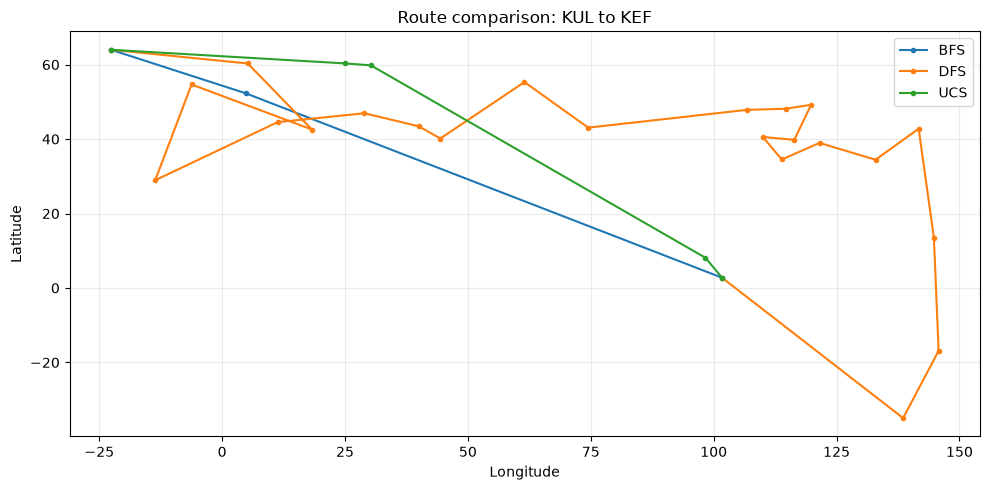
\includegraphics[width=.88\linewidth,height=5cm,keepaspectratio]{labs/visuals/01-notebook-reference.png}
\end{labvisual}
\begin{refoutput}
\begin{lstlisting}[style=utpterminal]
Saved: ['metrics.csv', 'route_comparison.png']
\end{lstlisting}
\end{refoutput}

\textbf{Read the result.} Regenerate this plot rather than copying it. Check the axes and the three routes; this saved figure is a reference, not evidence of your own run.
\end{labanswer}

\begin{yourturn}
Add new cells at the end of the notebook for these three tasks, and record your numbers before reading the expected findings.
\begin{enumerate}
  \item \textbf{Try a new query.} Run all three algorithms from \texttt{JFK} to \texttt{SYD} and record hops, kilometres and expansions.
  \item \textbf{Does direction matter?} Run BFS and UCS from \texttt{KEF} back to \texttt{KUL} and compare with the outward results. Is the best route back the same route reversed?
  \item \textbf{Check your warm-up.} Type in the graph of \figref{fig:ucs-vs-bfs} and compare with your hand trace. Then remove the edge from D to G and predict what BFS returns.
\end{enumerate}
\begin{lstlisting}[style=utppython]
tiny = {"A": [("B", 1.0), ("C", 4.0)], "B": [("D", 3.0), ("E", 2.0)], "C": [("F", 5.0)],
        "D": [("G", 4.0)], "E": [("G", 1.0)], "F": [("G", 2.0)], "G": []}
print(bfs(tiny, "A", "G").path, ucs(tiny, "A", "G").path)
\end{lstlisting}
\end{yourturn}

\begin{expectedfindings}
\begin{enumerate}
  \item BFS: 2 hops, 23,093~km via AUH, 537 expanded. DFS: 45 hops, 64,251~km. UCS: 2 hops, 16,035~km via LAX, 3,097 expanded. BFS stops at the first two-leg route it meets, 7,000~km too long.
  \item BFS: 2 hops via AMS, 12,274~km. UCS: 4 hops via HEL, LED and TAS, 11,478~km, which is not the outward UCS route reversed. Routes are directed, so a route out does not guarantee the same route back.
  \item BFS returns A--B--D--G at cost 8 and UCS returns A--B--E--G at cost 4. With the edge from D to G removed, BFS also returns A--B--E--G, because that is now the first three-edge route it reaches.
\end{enumerate}
\end{expectedfindings}

\begin{troubleshoot}
\begin{description}
  \item[\texttt{ModuleNotFoundError: utils}] Jupyter was not started from \texttt{all\_experiments/}. Restart it from there, or run the script from the course folder.
  \item[\texttt{FileNotFoundError}] A data file is missing or misnamed. Match Chapter~\ref{ch:toolkit}'s names, capitals too.
  \item[Different counts from the reference] Use the supplied data files and an unedited \texttt{utils/core.py}. Runtimes vary by machine; hops, kilometres and expansions should not.
\end{description}
\end{troubleshoot}

\begin{verification}
\begin{itemize}
  \item The cleaned graph has 6,464 usable airports and 37,337 unique directed routes.
  \item Every BFS, DFS and UCS path uses real routes, and its cost is the sum of its legs.
  \item BFS returns the fewest hops and UCS the shortest distance on every query; UCS finds the 11,461~km KUL$\to$KEF route.
  \item Reversing the neighbour order changes the DFS route, and you can explain why.
  \item \texttt{results/lab01/} holds \texttt{metrics.csv} and \texttt{route\_comparison.png}.
\end{itemize}
\end{verification}

\begin{labdeliverable}
\begin{itemize}
  \item Restart the kernel and run all cells without errors.
  \item Submit the executed notebook, including your \emph{Your turn} cells, and the generated \texttt{results/lab01/} folder.
  \item Add a short conclusion: which method minimises hops, which minimises distance, why DFS changes with neighbour order, and which effort measure is comparable across computers.
\end{itemize}
\end{labdeliverable}


\labsection{1}{Search Foundations on an Airline Network}{sec:lab01-search}

\begin{labproject}{Build and compare BFS, DFS, and Uniform-Cost Search}
\textbf{Read first.} Chapter~\ref{ch:uninformed}. Chapters~\ref{ch:toolkit} and~\ref{ch:git-submission} set up your tools.\\
\textbf{Goal.} Run BFS, DFS and UCS on one cleaned graph, verify every path, and explain why the algorithms disagree.\\
\textbf{Scenario.} Build a route planner over real airline connections and compare route quality with search effort.\\
\textbf{Data.} \texttt{all\_datasets/lab01-03\_airports.csv} and \texttt{lab01-03\_routes.csv}.\\
\textbf{Notebook.} \texttt{all\_experiments/lab01\_search\_foundations\_worked.ipynb}; Labs 1--3 share \texttt{all\_experiments/utils/}.\\
\textbf{Hand in.} The executed notebook, the \texttt{results/lab01/} folder and a short conclusion, as listed in the checklist at the end of this sheet.
\end{labproject}

\begin{labmode}
\begin{enumerate}
  \item Activate your course environment (Chapter~\ref{ch:toolkit}) and confirm that both data files are in \texttt{all\_datasets/}.
  \item Warm up on the robot's maze, which needs no data. From the course folder, run the command below. Its last line must read \texttt{Every number above matches the book.}
  \item Start Jupyter from \texttt{all\_experiments/}, open the notebook, and choose \textbf{Restart Kernel and Run All Cells}. Everything runs in a few seconds.
\end{enumerate}
\begin{lstlisting}[style=utpterminal]
python all_experiments/demo_robot_maze.py
cd all_experiments
jupyter lab
\end{lstlisting}
Prefer a plain script? From the course folder, \texttt{python all\_experiments/lab01\_search\_foundations\_worked.py} runs the same code and writes the same evidence.
\end{labmode}

\courselabflow{Clean routes}{Choose frontier}{Search routes}{Verify paths}


\labroutine

\begin{yourturn}
\textbf{Warm-up on paper.} Before touching the airline data, trace BFS and UCS by hand on the seven-node graph of \figref{fig:ucs-vs-bfs}, writing out the frontier after each expansion. You will check your trace with code at the end of this sheet.
\end{yourturn}

\textbf{Setup.} Run the imports and path setup first, and keep this kernel state for the later questions. In the script version the first seven lines also set the working directory, so that relative paths resolve.
\lstinputlisting[style=utppython,firstline=1,lastline=7]{all_experiments/lab01_search_foundations_worked.py}
\lstinputlisting[style=utppython,firstline=8,lastline=19]{all_experiments/lab01_search_foundations_worked.py}

\begin{labquestion}{1}{Load and validate the graph}
Load the airport and route files, keep only airports with a valid IATA code and coordinates, drop routes whose endpoints are unusable, and collapse duplicate routes. Report how many rows survive each step and show the three standard queries.
\end{labquestion}
\begin{labanswer}
\courselabtrace{One graph, different objectives}{BFS}{FIFO frontier; minimise hops}{UCS}{Priority by accumulated kilometres}{Check}{Every consecutive edge must exist}

\lstinputlisting[style=utppython,firstline=21,lastline=25]{all_experiments/lab01_search_foundations_worked.py}
\begin{refoutput}
\begin{lstlisting}[style=utpterminal]
airport_rows         10668      valid_airports        6464
route_rows           67663      unique_valid_routes  37337
removed_route_rows   30326
Queries:  Q1 KUL -> KEF     Q2 SIN -> EZE     Q3 NRT -> CPT
\end{lstlisting}
\end{refoutput}

\textbf{What it means.} Of 10,668 airport rows, 6,464 have a usable code and coordinates; of 67,663 route rows, 37,337 unique directed routes connect two usable airports. Every algorithm below runs on this same graph, so their results can be compared.
\end{labanswer}

\begin{labquestion}{2}{Define the edge cost}
BFS and DFS count every route as one step. UCS needs a number: the great-circle (Haversine) distance in kilometres between the two airports. Show the first five routes out of KUL with their distances, and the straight-line distance from KUL to KEF.
\end{labquestion}
\begin{labanswer}
\lstinputlisting[style=utppython,firstline=27,lastline=33]{all_experiments/lab01_search_foundations_worked.py}
\begin{refoutput}
\begin{lstlisting}[style=utpterminal]
KUL has 112 outgoing routes
Great-circle distance KUL -> KEF: 11,316 km (no direct route exists)
\end{lstlisting}
\end{refoutput}

\textbf{What it means.} Each edge carries the distance between its endpoints, computed once when the graph is built. Counting steps (BFS, DFS) and summing kilometres (UCS) are two different questions asked of the same graph.
\end{labanswer}

\textbf{Connect it to the chapter.} The next question runs the loop below three times. Only the highlighted box differs between the three algorithms.
% Reused from chapters/01-uninformed-search.tex
\begin{labvisual}{Recall the chapter model}
\begin{labgraphic}
\begin{tikzpicture}[font=\small]
\node[utpbox,minimum width=2.3cm] (start) at (0,0) {Start\\state};
\node[utpbox,minimum width=2.6cm,fill=UTPPaleOrange,draw=UTPOrange,line width=1pt]
  (pick) at (3.6,0) {\textbf{Select from}\\\textbf{frontier}};
\node[utpbox,minimum width=2.4cm] (goal) at (7.2,0) {Goal\\test?};
\node[utpbox,minimum width=2.6cm,fill=UTPPaleTeal,draw=UTPGreen] (done) at (10.7,0) {Return\\the path};
\node[utpbox,minimum width=2.6cm] (expand) at (7.2,-2.1) {Generate\\successors};
\node[utpbox,minimum width=2.6cm] (vis) at (3.6,-2.1) {Not already\\seen?};

\draw[utparrow] (start)--(pick);
\draw[utparrow] (pick)--(goal);
\draw[utparrow] (goal)--(done) node[midway,above,utplabel,color=UTPGreen] {yes};
\draw[utparrow] (goal)--(expand) node[midway,right,utplabel,color=UTPRed] {no};
\draw[utparrow] (expand)--(vis);
\draw[utparrow] (vis) -- (pick) node[midway,right,utplabel,color=UTPGreen] {keep};
\node[utplabel,anchor=south,align=center,color=UTPOrange] at (3.6,0.72)
  {\textbf{the only line that changes:} FIFO / LIFO / min-cost};
\node[utplabel,anchor=east,align=right] at (2.15,-2.1) {discard\\duplicates};
\end{tikzpicture}
\end{labgraphic}\end{labvisual}


\begin{labquestion}{3}{Run BFS, DFS and UCS on the three standard queries}
Record path, hops, distance, expanded nodes, maximum frontier and runtime for every algorithm and query, and save the table as \texttt{metrics.csv}. \emph{Predict first:} which algorithm will expand the most airports, and which will use the most legs?
\end{labquestion}
\begin{labanswer}
\lstinputlisting[style=utppython,firstline=35,lastline=44]{all_experiments/lab01_search_foundations_worked.py}
\begin{refoutput}
\begin{lstlisting}[style=utpterminal]
query algorithm hops        km expanded max_frontier
Q1    BFS          2  12274.32      284         1679
Q1    DFS         23  41767.82     2112          859
Q1    UCS          4  11461.35     1851          616
Q2    BFS          2  21976.11      233         1629
Q2    DFS         39  65213.84      904          858
Q2    UCS          3  17817.36     3002          620
Q3    BFS          2  19005.89      173         1727
Q3    DFS         64  91541.43     1414          785
Q3    UCS          3  14813.32     3042         1018
\end{lstlisting}
\end{refoutput}

\textbf{What it means.} BFS always returns the fewest hops (two legs on every query), UCS always returns the shortest distance, and DFS returns a long, winding route because it follows the first neighbour deeply. Expanded-node counts are the stable measure of effort; runtimes vary from machine to machine.
\end{labanswer}

\begin{labquestion}{4}{Verify every path independently}
A reported path is only evidence if it can be checked. Confirm that every consecutive pair of airports in every path is a real route, and recompute each path cost by summing the edge distances.
\end{labquestion}
\begin{labanswer}
Here is what the verification loop does for one path:
\courselabtrace{Verify an airline path independently}{1. Input / state}{Split the saved path into airport codes; edge\_km maps each source to its neighbours and distances.}{2. Operation}{For every adjacent pair a, b, confirm b is in edge\_km[a], then add edge\_km[a][b].}{3. Check}{Compare the sum with path\_cost\_km; len(path) - 1 is the hop count.}


\lstinputlisting[style=utppython,firstline=46,lastline=54]{all_experiments/lab01_search_foundations_worked.py}
\begin{refoutput}
\begin{lstlisting}[style=utpterminal]
Verified 9 paths: every leg exists and every cost matches its edge sum
\end{lstlisting}
\end{refoutput}

\textbf{What it means.} All nine paths use real routes and their costs equal the sum of their edge distances, so the metrics table can be trusted. The loader already removed unusable endpoints, yet verification still checks the returned edges: a bug in the search would show up here.
\end{labanswer}

\begin{labquestion}{5}{Compare the objectives}
Show hops and distance side by side for the three algorithms. Then run DFS again with every neighbour list reversed, to show that its answer depends on neighbour order.
\end{labquestion}
\begin{labanswer}
\lstinputlisting[style=utppython,firstline=56,lastline=62]{all_experiments/lab01_search_foundations_worked.py}
\begin{refoutput}
\begin{lstlisting}[style=utpterminal]
Q1 DFS: 23 hops with the original order, 8 with the reversed order
Q2 DFS: 39 hops with the original order, 41 with the reversed order
Q3 DFS: 64 hops with the original order, 39 with the reversed order
\end{lstlisting}
\end{refoutput}

\textbf{What it means.} BFS minimises the number of legs, so a two-leg route through a distant hub (KUL $\rightarrow$ AMS $\rightarrow$ KEF) wins even though UCS finds a four-leg route that is over 800~km shorter. Fewest legs and fewest kilometres are different objectives. DFS changes its answer as soon as the neighbour order changes, because it commits to the first branch it sees; it guarantees neither objective.
\end{labanswer}

\begin{labquestion}{6}{Save the evidence}
Plot the three KUL $\rightarrow$ KEF routes and save the figure next to \texttt{metrics.csv}.
\end{labquestion}
\begin{labanswer}
\lstinputlisting[style=utppython,firstline=64,lastline=68]{all_experiments/lab01_search_foundations_worked.py}
\begin{labvisual}{Reference plot from the supplied notebook}
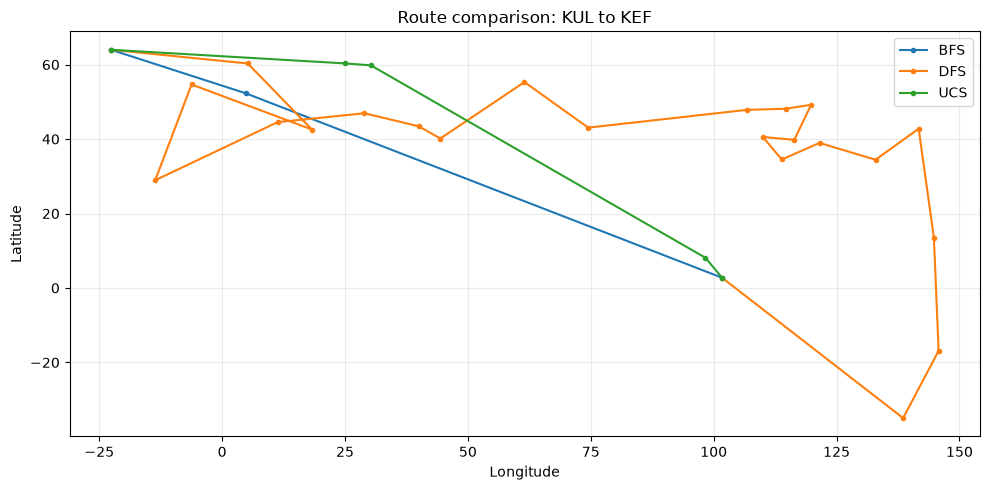
\includegraphics[width=.88\linewidth,height=5cm,keepaspectratio]{labs/visuals/01-notebook-reference.png}
\end{labvisual}
\begin{refoutput}
\begin{lstlisting}[style=utpterminal]
Saved: ['metrics.csv', 'route_comparison.png']
\end{lstlisting}
\end{refoutput}

\textbf{Read the result.} Regenerate this plot rather than copying it. Check the axes and the three routes; this saved figure is a reference, not evidence of your own run.
\end{labanswer}

\begin{yourturn}
Add new cells at the end of the notebook for these three tasks, and record your numbers before reading the expected findings.
\begin{enumerate}
  \item \textbf{Try a new query.} Run all three algorithms from \texttt{JFK} to \texttt{SYD} and record hops, kilometres and expansions.
  \item \textbf{Does direction matter?} Run BFS and UCS from \texttt{KEF} back to \texttt{KUL} and compare with the outward results. Is the best route back the same route reversed?
  \item \textbf{Check your warm-up.} Type in the graph of \figref{fig:ucs-vs-bfs} and compare with your hand trace. Then remove the edge from D to G and predict what BFS returns.
\end{enumerate}
\begin{lstlisting}[style=utppython]
tiny = {"A": [("B", 1.0), ("C", 4.0)], "B": [("D", 3.0), ("E", 2.0)], "C": [("F", 5.0)],
        "D": [("G", 4.0)], "E": [("G", 1.0)], "F": [("G", 2.0)], "G": []}
print(bfs(tiny, "A", "G").path, ucs(tiny, "A", "G").path)
\end{lstlisting}
\end{yourturn}

\begin{expectedfindings}
\begin{enumerate}
  \item BFS: 2 hops, 23,093~km via AUH, 537 expanded. DFS: 45 hops, 64,251~km. UCS: 2 hops, 16,035~km via LAX, 3,097 expanded. BFS stops at the first two-leg route it meets, 7,000~km too long.
  \item BFS: 2 hops via AMS, 12,274~km. UCS: 4 hops via HEL, LED and TAS, 11,478~km, which is not the outward UCS route reversed. Routes are directed, so a route out does not guarantee the same route back.
  \item BFS returns A--B--D--G at cost 8 and UCS returns A--B--E--G at cost 4. With the edge from D to G removed, BFS also returns A--B--E--G, because that is now the first three-edge route it reaches.
\end{enumerate}
\end{expectedfindings}

\begin{troubleshoot}
\begin{description}
  \item[\texttt{ModuleNotFoundError: utils}] Jupyter was not started from \texttt{all\_experiments/}. Restart it from there, or run the script from the course folder.
  \item[\texttt{FileNotFoundError}] A data file is missing or misnamed. Match Chapter~\ref{ch:toolkit}'s names, capitals too.
  \item[Different counts from the reference] Use the supplied data files and an unedited \texttt{utils/core.py}. Runtimes vary by machine; hops, kilometres and expansions should not.
\end{description}
\end{troubleshoot}

\begin{verification}
\begin{itemize}
  \item The cleaned graph has 6,464 usable airports and 37,337 unique directed routes.
  \item Every BFS, DFS and UCS path uses real routes, and its cost is the sum of its legs.
  \item BFS returns the fewest hops and UCS the shortest distance on every query; UCS finds the 11,461~km KUL$\to$KEF route.
  \item Reversing the neighbour order changes the DFS route, and you can explain why.
  \item \texttt{results/lab01/} holds \texttt{metrics.csv} and \texttt{route\_comparison.png}.
\end{itemize}
\end{verification}

\begin{labdeliverable}
\begin{itemize}
  \item Restart the kernel and run all cells without errors.
  \item Submit the executed notebook, including your \emph{Your turn} cells, and the generated \texttt{results/lab01/} folder.
  \item Add a short conclusion: which method minimises hops, which minimises distance, why DFS changes with neighbour order, and which effort measure is comparable across computers.
\end{itemize}
\end{labdeliverable}


\chapter{Informed Search: Greedy Best-First Search and A*}
\label{ch:informed}

\chapterguide%
  {Trace BFS, DFS and UCS (\chapref{ch:uninformed}) and explain what a priority queue does.}
  {define a heuristic and compute $g$, $h$ and $f$ for a state; trace Greedy Best-First Search and A$^\star$; decide whether a heuristic is admissible and why that matters; explain why a sharper guess saves work; and read the effort-versus-quality trade-off in Lab~2's tables.}

Look at where UCS went on the rainy maze. It spread evenly in every direction, even away from the charger, and expanded 47 of the 48 cells. It only counts the battery it has spent, so it has no idea which way the charger is. On the airline network the same blindness costs 1,851 expanded airports for the route from Kuala Lumpur to Keflav\'ik.

If you were standing in that maze you would head towards the charger, because you can roughly see where it is. This chapter gives the search that same sense of direction: a \term{heuristic}, a quick guess of how far is left. Lab~2 then measures what the guess does to search effort and to route quality.

\section{A guess of what is left}

Give the robot a simple guess. For any cell, count the steps across plus the steps up or down to the charger, and pretend walls and puddles do not exist. From the robot's cell at $(5,1)$ that is 8 columns across and 3 rows up, so its guess is 11. Do this for every cell and you get a number in each one, 0 on the charger and bigger further away (\figref{fig:manhattan}). In code it is one line:

\lstinputlisting[style=utppython,firstline=56,lastline=58]{all_experiments/demo_robot_maze.py}

\begin{utpfig}[The Manhattan guess]{The guess for every cell: rows apart plus columns apart, ignoring what is in the way. The robot's cell guesses 11, but the cheapest real route in the rain costs 13, because the guess cannot see walls or puddles.}{fig:manhattan}
\begin{tikzpicture}
\renewcommand{\mzstep}{4}
\mazegrid[0.62]{h}{\mazeguess}
\mazepins{h}
\node[anchor=west,align=left,text width=5.6cm,font=\small\color{UTPNavy}] at ($(h-3-9.east)+(0.45,0)$) {%
  \textbf{Two everyday guesses}\\[3pt]
  This count is the \term{Manhattan distance}, named after counting blocks in a city laid out on a grid.\\[3pt]
  On a map you would use the straight-line distance, \emph{as the crow flies}. Lab~2 uses that one for airports. It ignores what lies in the way, too.};
\end{tikzpicture}
\end{utpfig}

A guess like this is written $h(n)$. It is quick to work out and it is only an estimate. A search that uses one is called \term{informed}; BFS and UCS, which have no guess, are \term{uninformed}, or blind.

\section{Three quantities on one path}

Every informed method reasons about a frontier state $n$ using up to three numbers:

\begin{utptable}
\begin{tabularx}{\linewidth}{@{}
  >{\centering\arraybackslash\bfseries\leavevmode\color{UTPNavy}}m{0.14\linewidth}
  X
  >{\centering\arraybackslash}m{0.20\linewidth}@{}}
\toprule
\rowcolor{UTPPaleBlue!92}
\utpth{Quantity} & \utpth{Meaning} & \utpth{Used by} \\
\midrule
$g(n)$ & Exact cost of the cheapest known path from the start to $n$: what you have already spent & UCS, A$^\star$ \\
$h(n)$ & Estimated cost from $n$ to the goal: a guess of what is left & GBFS, A$^\star$ \\
$f(n)=g(n)+h(n)$ & Estimated total cost of a whole trip that passes through $n$ & A$^\star$ \\
\bottomrule
\end{tabularx}
\end{utptable}

\begin{analogy}
On a road trip, the odometer tells you how far you have driven and the map tells you roughly how far is left. The odometer is exact and backward-looking; it is $g$. The map is an estimate and forward-looking; it is $h$. Add them and you have a fair estimate of the whole trip, which is the number you would use to compare two possible routes.
\end{analogy}

\figref{fig:fgh} separates known cost from estimated remaining cost. UCS uses the former, GBFS the latter, and A$^\star$ both.

\begin{utpfig}[The three quantities $g$, $h$, and $f$]{$f(n)=g(n)+h(n)$ combines known cost with estimated remaining cost. UCS prioritises $g$, GBFS $h$, and A$^\star$ their sum.}{fig:fgh}
\begin{tikzpicture}[font=\small,
  method/.style={rounded corners=2mm,text width=2.75cm,minimum height=1.02cm,
                 align=center,font=\scriptsize\color{UTPNavy},inner sep=1.5mm,
                 line width=0.75pt}]
\node[utpnodedone,minimum size=9mm] (S) at (0,0) {S};
\node[utpnodehot,minimum size=9mm] (N) at (4,0) {$n$};
\node[utpnode,minimum size=9mm,fill=UTPPaleTeal,draw=UTPGreen] (G) at (8,0) {G};
\draw[utpedge,draw=UTPBlue,line width=1.3pt]
  (S) -- (1.15,0.48) -- (2.55,-0.32) -- (N);
\draw[utpedge,draw=UTPMuted!55,line width=1.2pt,dashed] (N) -- (G);
\draw[utpbrace,draw=UTPBlue] (-0.3,0.92) -- (4,0.92);
\draw[utpbrace,draw=UTPOrange] (4,0.92) -- (8.3,0.92);
\node[utplabel,anchor=south,color=UTPBlue,align=center] at (1.85,1.22)
  {$g(n)$ --- exact cost\\from start to $n$};
\node[utplabel,anchor=south,color=UTPOrange,align=center] at (6.15,1.22)
  {$h(n)$ --- estimated cost\\from $n$ to goal};
\node[method,draw=UTPBlue,fill=UTPPaleBlue] (ucs) at (0.75,-1.65)
  {\textbf{UCS}\\priority $g(n)$\\actual cost only};
\node[method,draw=UTPOrange,fill=UTPPaleOrange] (gbfs) at (4,-1.65)
  {\textbf{GBFS}\\priority $h(n)$\\estimate only};
\node[method,draw=UTPGreen,fill=UTPPaleTeal] (astar) at (7.25,-1.65)
  {\textbf{A*}\\priority $f(n)=g(n)+h(n)$\\combines both};
\end{tikzpicture}
\end{utpfig}

\section{Greedy best-first search: go where it looks closest}

The simplest way to use the guess is to take the cell whose guess is smallest, the one that \emph{looks} closest to the charger. That is \term{Greedy Best-First Search (GBFS)}: best-first because it always explores the best-looking cell, greedy because it only cares about getting closer right now. It uses the same priority queue as UCS. Only the number changes: UCS sorts by $g$, GBFS by $h$.

Walk it on the rainy maze. From the robot, the cells above and to the right both guess 10, and the one above joined first, so GBFS goes up. It climbs to $(2,1)$ on the charger's row, where the guess is 8, and meets a wall. The next best-looking cell is $(3,2)$, also guessing 8, so it steps straight into the first puddle without noticing and runs along the corridor from there, every step bringing the guess down by one. It never looks at the bottom of the maze.

GBFS reaches the charger after expanding only 13 cells, the least work of anything so far. But its route is the middle corridor at 19 units of battery, and the robot runs dry four cells short. GBFS looks only at what is left. It never counts what it has already spent.

\begin{workedexample}
On the airline network GBFS expands two airports for \texttt{KUL -> LHR -> KEF}: 12,500~km, 9\,\% above the optimum. London looks close to Iceland, but the first leg alone exceeds the optimal route through Phuket, St Petersburg and Helsinki. Its \texttt{NRT}$\to$\texttt{CPT} route is 6.7\,\% too long, and its \texttt{SIN}$\to$\texttt{EZE} route happens to be optimal.
\end{workedexample}

\begin{pitfall}
Because GBFS ignores $g$, a small $h$ can conceal an expensive path. How good its route is depends on what the graph looks like around the goal, so one good result proves nothing about the next query.
\end{pitfall}

\section{A* search: what you spent plus what is left}

Neither search does both jobs. UCS gets the robot home but looks at every cell. GBFS heads straight for the charger but runs out of battery. UCS counts what is spent, $g$. GBFS guesses what is left, $h$. So add them up, $f(n)=g(n)+h(n)$, and take the cell with the smallest $f$. That is \term{A$^\star$}, the same priority queue again, sorted by a third number. In \texttt{utils/core.py} the three algorithms share \texttt{best\_first}, and these lines are all that separates them:

\lstinputlisting[style=utppython,firstline=104,lastline=109]{all_experiments/utils/core.py}

\figref{fig:astar-cells} shows how to read the three numbers on a cell. Follow the first few picks on the rainy maze, keeping an eye on $(3,2)$.

\begin{utpfig}[Reading $g$, $h$ and $f$ on a cell]{Four cells from the first picks of A$^\star$ on the rainy maze. The big number is $f$, the sum of $g$ (top left) and $h$ (top right). Stepping into the puddle at $(3,2)$ costs 5, so its $f$ jumps to 15 and it waits behind every cell with $f=13$.}{fig:astar-cells}
\begin{tikzpicture}[font=\small]
\newcommand{\fcell}[7]{%
  \node[draw=#6,fill=#7,minimum width=1.92cm,minimum height=1.55cm,inner sep=0pt] (#1) at (#2,0) {};
  \node[anchor=north west,font=\scriptsize\color{UTPBlue},inner sep=2.5pt] at (#1.north west) {$g=#3$};
  \node[anchor=north east,font=\scriptsize\color{UTPOrange!85!black},inner sep=2.5pt] at (#1.north east) {$h=#4$};
  \node[font=\large\bfseries\color{UTPNavy}] at ($(#1.center)+(0,-0.16)$) {#5};
}
\fcell{a}{0}{0}{11}{11}{UTPOrange}{UTPPaleOrange}
\node[utplabel,anchor=north,align=center] at (a.south) {robot's cell\\$(5,1)$};
\fcell{b}{2.25}{1}{10}{11}{UTPBlue!55}{UTPPaleBlue}
\node[utplabel,anchor=north,align=center] at (b.south) {one step right\\$(5,2)$};
\fcell{c}{4.5}{2}{11}{13}{UTPBlue!55}{UTPPaleBlue}
\node[utplabel,anchor=north,align=center] at (c.south) {then one down\\$(6,2)$};
\fcell{d}{6.75}{7}{8}{15}{UTPTeal}{UTPTeal!30}
\node[utplabel,anchor=north,align=center] at (d.south) {first puddle\\$(3,2)$: $g=2+5$};
\node[anchor=west,align=left,text width=4.5cm,font=\scriptsize\color{UTPNavy}] at (8.0,0) {\textbf{Along the bottom row} every step adds 1 to $g$ and takes 1 off $h$, so $f$ stays at 13 all the way. A$^\star$ follows it and never expands the puddle.};
\end{tikzpicture}
\end{utpfig}

\begin{workedexample}
The first five picks of A$^\star$. Each cell added to the frontier is shown with its $f$.
\medskip

\centering\small
\begin{tabular}{@{}lll@{}}
\toprule
\rowcolor{UTPPaleBlue!92}
\utpth{Pick} & \utpth{Its $f$} & \utpth{Added to the frontier (with $f$)} \\
\midrule
$(5,1)$ & 11 & $(4,1)$ 11,\ \ $(5,2)$ 11,\ \ $(6,1)$ 13,\ \ $(5,0)$ 13 \\
$(4,1)$ & 11 & $(3,1)$ 11,\ \ $(4,0)$ 13 \\
$(5,2)$ & 11 & $(6,2)$ 13 \\
$(3,1)$ & 11 & $(2,1)$ 11,\ \ $(3,2)$ \textbf{15} (the puddle) \\
$(2,1)$ & 11 & $(1,1)$ 13,\ \ $(2,0)$ 13 \\
\bottomrule
\end{tabular}
\par\raggedright
\medskip
The frontier now holds several cells with $f=13$ and one with $f=15$. A$^\star$ clears every 13 first, and those cells lead along the bottom row to the charger.
\end{workedexample}

A$^\star$ reaches the charger with $g=13$. That is the route UCS found, but A$^\star$ expanded only 28 cells instead of 47 (\figref{fig:expansion}).

\begin{utpfig}[Cells expanded by UCS, GBFS, and A*]{The rainy maze solved three ways, with the same battery of 15. Blue cells were expanded. UCS spreads everywhere and finds the 13-unit route. GBFS barely explores, but its route costs 19 and the robot runs dry. A$^\star$ finds the 13-unit route and leaves the top and the corridor alone.}{fig:expansion}
\begin{tikzpicture}
\begin{scope}
\node[mztitle] at (1.8,0.48) {UCS (sorts on $g$)};
\mazegrid[0.40]{u}{\mazeucs}\mazeroute{u}{\routebottom}\mazepins{u}
\node[mznote,anchor=north] at (1.8,-2.65) {47 expanded, 13 units};
\end{scope}
\begin{scope}[xshift=5.2cm]
\node[mztitle] at (1.8,0.48) {GBFS (sorts on $h$)};
\mazegrid[0.40]{g}{\mazegreedy}\mazeroute[mzroutebad]{g}{\routecorridor}\mazepins{g}
\node[mznote,anchor=north] at (1.8,-2.65) {13 expanded, 19 units: runs dry};
\end{scope}
\begin{scope}[xshift=10.4cm]
\node[mztitle] at (1.8,0.48) {A* (sorts on $g+h$)};
\mazegrid[0.40]{a}{\mazeastar}\mazeroute{a}{\routebottom}\mazepins{a}
\node[mznote,anchor=north] at (1.8,-2.65) {28 expanded, 13 units};
\end{scope}
\end{tikzpicture}
\end{utpfig}

Why did A$^\star$ get to skip so much? Colour every cell by the best $f$ it can have, using the cheapest way to reach it (\figref{fig:fmap}). A$^\star$ expanded exactly the cells with $f\le13$, and every cell it skipped has $f\ge15$. The guess never exceeds the real remaining cost, because walls can only make a route longer and puddles can only make it dearer. So any route through a skipped cell costs at least 15, more than the 13 already in hand, and there was never a reason to look.

\begin{utpfig}[Why A* can skip cells]{Each cell shows the best possible $f=g+h$ on the rainy maze. Blue cells have $f\le13$ and are exactly the ones A$^\star$ expanded. Grey cells have $f\ge15$: any route through them must cost at least that, so with a 13-unit route in hand they can be ignored.}{fig:fmap}
\begin{tikzpicture}
\renewcommand{\mzdrawnumber}[1]{%
  \ifnum\mzv>13
    \node[mzcell,draw=UTPMuted!45,fill=UTPPaleGray,font=\scriptsize\color{UTPMuted}] (#1-\mzr-\mzc)
      at (\mzs*\mzc,-\mzs*\mzr) {\mzv};%
  \else
    \node[mzcell,draw=UTPBlue!50,fill=UTPBlue!24] (#1-\mzr-\mzc)
      at (\mzs*\mzc,-\mzs*\mzr) {\mzv};%
  \fi}
\mazegrid[0.62]{f}{\mazef}
\mazeroute{f}{\routebottom}
\mazelabels{f}{\mazef}
\mazepins{f}
\node[anchor=west,align=left,text width=5.6cm,font=\small\color{UTPNavy}] at ($(f-3-9.east)+(0.45,0)$) {%
  \textbf{A$^\star$'s trick}\\[3pt]
  What you have spent plus a guess of what is left that never runs high. A$^\star$ only explores cells that could still lie on the cheapest route.};
\end{tikzpicture}
\end{utpfig}

\begin{keyidea}
GBFS asks which frontier state \emph{looks} closest to the goal. A$^\star$ also accounts for the cost already paid and, with a suitable heuristic, guarantees the cheapest path.
\end{keyidea}

\begin{workedexample}
Suppose frontier state $X$ has $(g,h)=(5,3)$ and $Y$ has $(1,5)$. GBFS chooses $X$ because $3<5$. A$^\star$ chooses $Y$ because $f(Y)=6<f(X)=8$: the cheaper path so far is worth the extra estimated distance.
\end{workedexample}

\begin{libnote}
Peter Hart, Nils Nilsson and Bertram Raphael published A$^\star$ in 1968 at the Stanford Research Institute. They developed it for Shakey, one of the first mobile robots able to plan its own actions. Their example heuristic for cities joined by roads was the airline distance, the same as-the-crow-flies guess you will use in Lab~2. A$^\star$ with $h=0$ is exactly UCS, so A$^\star$ is Dijkstra's algorithm with a guess added.
\end{libnote}

\section{The one rule: never overestimate}

The guess made A$^\star$ faster, so why not trust it even more? Multiply every guess by three. On the robot's cell the guess of 11 becomes 33, far above the real cost of 13, and from every cell A$^\star$ now believes the charger is much further away than it is. The tripled guess is so much bigger than the battery spent that it decides almost every pick. A$^\star$ heads straight for the charger like GBFS, expands only 16 cells, and returns the 19-unit corridor. The robot runs dry again (\figref{fig:triple}).

\begin{utpfig}[Inflating the guess breaks the guarantee]{A$^\star$ on the rainy maze with the honest guess and with the guess multiplied by three. Trusting the guess too much saves 12 expansions and loses the cheapest route.}{fig:triple}
\begin{tikzpicture}
\begin{scope}
\node[mztitle] at (2.16,0.5) {$f=g+h$};
\mazegrid[0.48]{a}{\mazeastar}\mazeroute{a}{\routebottom}\mazepins{a}
\node[mznote,anchor=north] at (2.16,-3.15) {28 expanded, 13 units, reaches the charger};
\end{scope}
\begin{scope}[xshift=7.0cm]
\node[mztitle] at (2.16,0.5) {$f=g+3h$};
\mazegrid[0.48]{t}{\mazetriple}\mazeroute[mzroutebad]{t}{\routecorridor}\mazepins{t}
\node[mznote,anchor=north] at (2.16,-3.15) {16 expanded, 19 units, runs dry};
\end{scope}
\end{tikzpicture}
\end{utpfig}

\subsection{Admissibility and consistency}

So there is one rule. A heuristic is \term{admissible} when it never overestimates the cheapest remaining cost:
\[
h(n)\;\le\;h^\star(n)\quad\text{for every state } n,
\]
where $h^\star(n)$ is the true cost of the cheapest path from $n$ to the goal. If that holds, A$^\star$ is guaranteed to return a cheapest path. Our Manhattan guess qualifies: on the robot's cell it is 11 against a true 13.

A stronger and more convenient condition is \term{consistency}: for every edge $n\to n'$ of cost $c$, $h(n)\le c+h(n')$. In words, one step cannot make the guess drop by more than the step cost. Consistency implies admissibility and guarantees that the first time A$^\star$ pops a state, it has found the cheapest path to it, which is what allows the closed-set implementation in \texttt{utils} to skip re-expansions. Its picture is the triangle inequality (\figref{fig:triangle}).

\begin{utpfig}[Why a straight-line guess is consistent]{The direct line from $n$ to the goal can never be longer than going via $n'$ first. The same is true on a sphere, which is why the great-circle distance is a consistent heuristic for airline routes: no sequence of flights can beat flying straight there.}{fig:triangle}
\begin{tikzpicture}[font=\small]
\node[utpnodehot,minimum size=8mm] (N) at (0,0) {$n$};
\node[utpnode,minimum size=8mm] (P) at (3.1,1.55) {$n'$};
\node[utpnodedone,minimum size=8mm] (G) at (6.2,0) {G};
\draw[utpptr,draw=UTPBlue,line width=1pt] (N)--(P) node[midway,above left,utplabel,color=UTPBlue] {$c$: one real flight};
\draw[utpptr,draw=UTPOrange,dashed,line width=1pt] (P)--(G) node[midway,above right,utplabel,color=UTPOrange!85!black] {$h(n')$: straight line};
\draw[utpptr,draw=UTPOrange,dashed,line width=1pt] (N)--(G) node[midway,below,utplabel,color=UTPOrange!85!black] {$h(n)$: straight line};
\node[anchor=west,font=\small\color{UTPNavy}] at (7.2,0.7) {$h(n)\ \le\ c+h(n')$};
\end{tikzpicture}
\end{utpfig}

\begin{intuition}
An inadmissible heuristic makes A$^\star$ behave like GBFS: it trusts the estimate too much and commits to a branch before the cost evidence justifies it. Admissibility keeps the $g$ term in charge whenever the two disagree.
\end{intuition}

\subsection{The Haversine heuristic}

Any heuristic should be cheap to compute and use the same units as the path cost. For kilometre-based routes, use the great-circle distance to the goal, whether or not a direct flight exists. The \term{Haversine formula} computes it from latitude--longitude pairs:
\[
h(n)=2R\,\arcsin\!\sqrt{\sin^2\!\tfrac{\Delta\varphi}{2}+\cos\varphi_n\cos\varphi_{\text{goal}}\sin^2\!\tfrac{\Delta\lambda}{2}}
\]
with $R\approx6371$~km. The same formula gives every edge weight in the graph, so $h$ and $g$ are directly comparable. In Lab~2 the heuristic is a small function that fixes the goal and returns a function of the airport:

\lstinputlisting[style=utppython,firstline=36,lastline=41]{all_experiments/lab02_informed_search_worked.py}

\texttt{utils/core.py} accepts any state-to-number callable, so changing the heuristic requires no change to the search code.

Theory says Haversine is safe. Lab~2 checks it anyway: it runs Dijkstra backwards from each goal to get the exact cost $h^\star$, samples ten airports across the range for each of three goals, and confirms $h\le h^\star$. In \figref{fig:admissible}, every sampled point must lie on or below the diagonal.

\begin{utpfig}[Checking admissibility state by state]{A heuristic plotted against the true remaining cost, with illustrative points. Admissibility requires every point to lie on or below the dashed line. The red points overestimate and void the A$^\star$ guarantee. The Haversine heuristic in Lab~2 produces only green points, with slack from 0 up to about 26,000~km.}{fig:admissible}
\begin{tikzpicture}
\begin{axis}[
  width=0.62\linewidth, height=5.4cm,
  xlabel={true remaining cost $h^\star(n)$}, ylabel={heuristic $h(n)$},
  xmin=0, xmax=7, ymin=0, ymax=7.6,
  xtick={0,1,...,7}, ytick={0,2,4,6},
  axis lines=left, grid=major, grid style={draw=UTPPaleBlue},
  clip=false]
\addplot[draw=UTPMuted,dashed,thick] coordinates {(0,0) (7,7)};
\addplot[only marks,mark=*,mark size=2.4pt,UTPRed]
  coordinates {(4,7) (3,6) (1,2)};
\addplot[only marks,mark=*,mark size=2.4pt,UTPGreen]
  coordinates {(6,4) (2,2) (0,0) (5,3.2) (3.5,1.8)};
\node[font=\scriptsize\color{UTPMuted},anchor=west] at (axis cs:4.4,4.1) {$h=h^\star$};
\node[font=\scriptsize\color{UTPRed},anchor=west,align=left] at (axis cs:0.3,6.2)
  {above the line:\\overestimates};
\node[font=\scriptsize\color{UTPGreen},anchor=west,align=left] at (axis cs:4.6,1.4)
  {on or below:\\admissible};
\end{axis}
\end{tikzpicture}
\end{utpfig}

\subsection{Weighted A*: trading the guarantee for speed}

Sometimes a good answer now beats the best answer later. \term{Weighted A$^\star$} uses $g+w\,h$ with $w>1$, deliberately giving up the guarantee for a more goal-directed search. The tripled guess above was weighted A$^\star$ with $w=3$. At $w=1.5$, Lab~2 uses two, three and four expansions, with routes 7.1\,\%, 0\,\% and 0.8\,\% above optimum. Inflating $h$ discourages useful detours away from the goal, so the cost changes exactly when the best route takes one.

\section{A sharper guess means less work}

Not all admissible guesses are equally good. The 8-puzzle shows how much the quality of the guess matters. Here are two guesses for how many slides are left, both never overestimating:

\begin{description}
  \item[Misplaced tiles.] Count the tiles not on their home square. Every misplaced tile needs at least one slide.
  \item[Tile distance.] Add up each tile's Manhattan distance from its home square. Every tile needs at least that many slides.
\end{description}

\begin{utpfig}[Two guesses on one board]{The board traced by \texttt{demo\_sliding\_puzzle.py}, next to the goal. Seven tiles are misplaced, so the weak guess is 7. The small orange number on each tile is its distance from home, and these add up to the sharper guess of 16. The true answer is 22 slides.}{fig:puzzle-guess}
\begin{tikzpicture}[font=\small,
  tile/.style={utpcell,minimum width=0.92cm,minimum height=0.92cm,font=\normalsize\bfseries\color{UTPNavy}},
  gap/.style={utpdim,minimum width=0.92cm,minimum height=0.92cm},
  away/.style={circle,fill=UTPOrange,text=white,font=\tiny\bfseries,inner sep=1.1pt}]
\node[mztitle] at (0.92,0.85) {Traced board};
\foreach \t/\d/\c/\r in {8/3/0/0,2/0/1/0,6/2/0/1,1/2/1/1,7/3/2/1,4/1/0/2,3/3/1/2,5/2/2/2}{
  \node[tile] (t\t) at (0.92*\c,-0.92*\r) {\t};
  \node[away] at ($(t\t.north east)+(-0.13,-0.13)$) {\d};
}
\node[gap] at (1.84,0) {};
\node[mztitle] at (5.72,0.85) {Goal};
\foreach \t/\c/\r in {1/0/0,2/1/0,3/2/0,4/0/1,5/1/1,6/2/1,7/0/2,8/1/2}{
  \node[utpdone,minimum width=0.92cm,minimum height=0.92cm,font=\normalsize\bfseries\color{UTPNavy}] at ({4.8+0.92*\c},-0.92*\r) {\t};
}
\node[gap] at (6.64,-1.84) {};
\node[anchor=west,align=left,text width=5.2cm,font=\scriptsize\color{UTPNavy}] at (7.9,-0.92) {Tile distance: $3+0+2+2+3+1+3+2=16$.\\[3pt] Misplaced: every tile except 2, so 7.\\[3pt] Both are below the true 22, so both are admissible, and A$^\star$ finds a 22-slide solution with either.};
\end{tikzpicture}
\end{utpfig}

\begin{utptable}
\begin{tabularx}{\linewidth}{@{}>{\bfseries\leavevmode\color{UTPNavy}}m{0.34\linewidth}>{\centering\arraybackslash}X>{\centering\arraybackslash}X>{\centering\arraybackslash}X@{}}
\toprule
\rowcolor{UTPPaleBlue!92}
\utpth{Search on the traced board} & \utpth{Guess at the start} & \utpth{Slides returned} & \utpth{States expanded} \\
\midrule
BFS, no guess & --- & 22 & 89,296 \\
A$^\star$, misplaced tiles & 7 & 22 & 7,356 \\
A$^\star$, tile distance & 16 & 22 & 417 \\
\bottomrule
\end{tabularx}
\end{utptable}

Sixteen is much closer to the truth than seven, so A$^\star$ wastes far less time. Among admissible guesses, the larger the better: a guess that is closer to the true cost prunes more of the space without ever losing the guarantee.

\section{UCS, GBFS and A* side by side}

\begin{utptable}
\begin{tabularx}{\linewidth}{@{}
  >{\centering\arraybackslash\bfseries\leavevmode\color{UTPNavy}}m{0.14\linewidth}
  >{\centering\arraybackslash}m{0.14\linewidth}
  >{\centering\arraybackslash}m{0.16\linewidth}
  >{\centering\arraybackslash}m{0.17\linewidth}
  X@{}}
\toprule
\rowcolor{UTPPaleBlue!92}
\utpth{Method} & \utpth{Priority} & \utpth{Optimal?} & \utpth{Rainy maze} & \utpth{Behaviour in Lab~2} \\
\midrule
UCS & $g(n)$ & Yes & 47 cells, 13 units & Exact but blind: 1,851--3,042 expansions per query \\
GBFS & $h(n)$ & No & 13 cells, 19 units & 2--3 expansions; routes up to 9\,\% too long \\
A$^\star$ & $g(n)+h(n)$ & Yes, if $h$ consistent & 28 cells, 13 units & Same cost as UCS with 96\,\% fewer expansions \\
Weighted A$^\star$ & $g(n)+w\,h(n)$ & No & 16 cells, 19 units ($w=3$) & 2--4 expansions at $w=1.5$; routes up to 7\,\% too long \\
\bottomrule
\end{tabularx}
\end{utptable}

\begin{keyidea}
A$^\star$ combines low effort with optimality because its heuristic is consistent. UCS explores without guidance; GBFS reduces effort but gives up the guarantee.
\end{keyidea}

\section{Reading the lab's evidence}

\texttt{metrics.csv} records cost, hops, expansions, peak frontier, runtime and the \term{optimality gap}: the percentage by which a route costs more than the UCS route. A$^\star$ has zero gap on every query, and any positive GBFS or weighted A$^\star$ gap is the measured price of speed. \texttt{heuristic\_check.csv} compares $h$ with $h^\star$ for thirty sampled airports. A single failed check would invalidate the admissibility claim.

\begin{chapterrecap}
\begin{itemize}
  \item A heuristic $h(n)$ is a cheap guess of the cost left. $g(n)$ is what you have spent, and $f(n)=g(n)+h(n)$ estimates the whole trip.
  \item UCS, GBFS and A$^\star$ are one priority queue sorted by $g$, $h$ and $g+h$. GBFS is quick and can be badly wrong; A$^\star$ is both quick and correct.
  \item The one rule: an admissible heuristic never overestimates. Break it, as weighted A$^\star$ does on purpose, and speed comes at the price of the guarantee.
  \item Among admissible heuristics, the one closest to the true cost does the least work.
\end{itemize}
\end{chapterrecap}

\begin{quickcheck}
\begin{enumerate}
  \item Which quantity does GBFS ignore that A$^\star$ uses, and which failure in Lab~2 does that explain?
  \item Frontier states $X$ and $Y$ have $(g,h)=(8,2)$ and $(3,6)$. Which does UCS expand first? GBFS? A$^\star$?
  \item Why must $h$ be expressed in the same units as the edge costs?
  \item Lab~2 computes $h^\star$ by running Dijkstra on the \emph{reversed} graph from the goal. Why reversed?
  \item Weighted A$^\star$ with $w=1.5$ changed the cost for KUL$\to$KEF but not for SIN$\to$EZE. What property of the SIN$\to$EZE route explains this?
  \item On the rainy maze, cell $(3,2)$ has $g=7$ and $h=8$. Why does A$^\star$ never expand it, even though it joined the frontier early?
\end{enumerate}
\end{quickcheck}

\begin{checkanswers}
\begin{enumerate}
  \item GBFS ignores $g$, the cost already paid. That is why it jumps to London for KUL$\to$KEF: the first leg alone costs more than the whole optimal route, but London \emph{looks} close to Iceland.
  \item UCS expands $Y$ ($g=3<8$). GBFS expands $X$ ($h=2<6$). A$^\star$ expands $Y$ ($f(Y)=9<f(X)=10$).
  \item Because $f=g+h$ adds them. If $h$ were in miles and $g$ in kilometres, $h$ would simply be weaker; in metres it would be 1,000 times too large and A$^\star$ would behave like GBFS.
  \item Dijkstra from a start gives the cheapest cost \emph{from} it to every state. Routes are one-way, so reversing every edge and starting at the goal gives the cheapest cost \emph{to} the goal from every airport, which is what $h^\star$ is.
  \item The optimal SIN$\to$JNB$\to$GRU$\to$EZE route heads towards the goal on every leg, so inflating $h$ does not make any of its legs look worse. The optimal KUL route detours through Phuket, and an inflated $h$ penalises that detour.
  \item Its $f$ is 15. The charger is reached along cells with $f=13$, and A$^\star$ always serves the smallest $f$ first, so the charger comes off the list before the puddle's turn arrives.
\end{enumerate}
\end{checkanswers}

\labsection{2}{Heuristic Search on the Airline Network}{sec:lab02-informed}

\begin{labproject}{Compare UCS, Greedy Best-First Search, and A$^\star$}
\textbf{Coverage.} Chapter~\ref{ch:informed}.\\
\textbf{Goal.} Run GBFS and A$^\star$ with a Haversine heuristic, check admissibility, and measure quality against search effort.\\
\textbf{Scenario.} Improve the Lab~1 planner by adding geographic knowledge while keeping a clear quality baseline.\\
\textbf{Data.} The Lab~1 OpenFlights files.\\
\textbf{Notebook.} \texttt{all\_experiments/lab02\_informed\_search\_worked.ipynb} and the shared \texttt{all\_experiments/utils/}.
\end{labproject}

\noindent\textbf{Setup cell.}
\begin{lstlisting}[style=utppython]
from heapq import heappop, heappush
from pathlib import Path

import numpy as np
import pandas as pd
import matplotlib.pyplot as plt
from IPython.display import display

from utils import ucs, gbfs, astar, haversine_km, load_openflights

ROOT = Path.cwd().parent
DATA = ROOT / "all_datasets"
RESULTS = ROOT / "results" / "lab02"
RESULTS.mkdir(parents=True, exist_ok=True)

_, _, coords, graph, _ = load_openflights(DATA / "lab01-03_airports.csv", DATA / "lab01-03_routes.csv")
queries = pd.read_csv("utils/search_queries.csv").head(3)
display(queries)
\end{lstlisting}

\begin{labquestion}{1}{Establish the baseline}
Run UCS for the three standard queries. UCS is exact for non-negative costs, so its cost is the reference every informed method is judged against.
\end{labquestion}

\begin{labanswer}
\begin{lstlisting}[style=utppython]
def report(name, query, result):
    print(f"{query.query_id} {name:<5} {result.path_cost_km:>9,.1f} km  {result.expanded:>5} expanded   {' -> '.join(result.path)}")


baseline = {}
for query in queries.itertuples():
    baseline[query.query_id] = ucs(graph, query.start, query.goal)
    report("UCS", query, baseline[query.query_id])
\end{lstlisting}
\expectedoutput
\begin{lstlisting}[style=utpterminal]
Q1 UCS    11,461.3 km   1851 expanded   KUL -> HKT -> LED -> HEL -> KEF
Q2 UCS    17,817.4 km   3002 expanded   SIN -> JNB -> GRU -> EZE
Q3 UCS    14,813.3 km   3042 expanded   NRT -> HKG -> MRU -> CPT
\end{lstlisting}
UCS reproduces the Lab~1 distances. These are the optimal costs; an informed method that returns more has traded quality for speed. The small \texttt{report} helper prints every result in the same shape, so the rows below line up with these.
\end{labanswer}

\begin{labquestion}{2}{Implement the heuristic and run GBFS and A$^\star$}
Use the great-circle distance from the current airport to the goal as $h(n)$. GBFS orders the frontier by $h$ alone; A$^\star$ by $g+h$. Write the heuristic as a function that fixes the goal, then run both algorithms.
\end{labquestion}

\begin{labanswer}
\begin{lstlisting}[style=utppython]
def heuristic_to(goal, weight=1.0):
    """h(airport) = weight x great-circle distance from the airport to the goal."""
    def h(airport):
        return weight * haversine_km(coords[airport]["latitude"], coords[airport]["longitude"],
                                     coords[goal]["latitude"], coords[goal]["longitude"])
    return h


informed = {}
for query in queries.itertuples():
    h = heuristic_to(query.goal)
    informed[query.query_id, "GBFS"] = gbfs(graph, query.start, query.goal, h)
    informed[query.query_id, "A*"] = astar(graph, query.start, query.goal, h)
    report("GBFS", query, informed[query.query_id, "GBFS"])
    report("A*", query, informed[query.query_id, "A*"])
\end{lstlisting}
\expectedoutput
\begin{lstlisting}[style=utpterminal]
Q1 GBFS   12,500.5 km      2 expanded   KUL -> LHR -> KEF
Q1 A*     11,461.3 km     69 expanded   KUL -> HKT -> LED -> HEL -> KEF
Q2 GBFS   17,817.4 km      3 expanded   SIN -> JNB -> GRU -> EZE
Q2 A*     17,817.4 km    151 expanded   SIN -> JNB -> GRU -> EZE
Q3 GBFS   15,811.3 km      3 expanded   NRT -> DOH -> JNB -> CPT
Q3 A*     14,813.3 km     63 expanded   NRT -> HKG -> MRU -> CPT
\end{lstlisting}
A$^\star$ returns exactly the UCS cost on every query while expanding far fewer states. GBFS expands only a handful of states, but two of its three routes are longer because it ignores the distance already travelled. \texttt{heuristic\_to} returns a function: the algorithms in \texttt{utils} accept any callable that maps a state to a number.
\end{labanswer}

\begin{labquestion}{3}{Check admissibility empirically}
An admissible heuristic never overestimates the true remaining cost. Run Dijkstra once on the reversed graph to get the exact cost from every airport \emph{to} the goal, then compare $h$ with that exact cost for ten airports spread across the range. Save \texttt{heuristic\_check.csv}.
\end{labquestion}

\begin{labanswer}
\begin{lstlisting}[style=utppython]
def reverse(graph):
    reversed_graph = {airport: [] for airport in graph}
    for airport, neighbours in graph.items():
        for neighbour, cost in neighbours:
            reversed_graph[neighbour].append((airport, cost))
    return reversed_graph


def cost_to_all(graph, start):
    """Dijkstra: cheapest cost from start to every reachable state."""
    best = {start: 0.0}
    frontier = [(0.0, start)]
    while frontier:
        cost, state = heappop(frontier)
        if cost > best[state]:
            continue
        for neighbour, edge in graph[state]:
            if cost + edge < best.get(neighbour, np.inf):
                best[neighbour] = cost + edge
                heappush(frontier, (cost + edge, neighbour))
    return best


reversed_graph = reverse(graph)
checks = []
for query in queries.itertuples():
    exact = cost_to_all(reversed_graph, query.goal)          # exact cost-to-go for every airport
    h = heuristic_to(query.goal)
    airports = sorted((a for a in exact if a != query.goal), key=exact.get)   # nearest first
    for airport in [airports[i] for i in np.linspace(0, len(airports) - 1, 10, dtype=int)]:
        checks.append({"query_id": query.query_id, "airport": airport, "goal": query.goal,
                       "haversine_km": h(airport), "shortest_route_km": exact[airport]})

check = pd.DataFrame(checks)
check["slack_km"] = check.shortest_route_km - check.haversine_km
check["admissible"] = check.slack_km >= -1e-6
check.to_csv(RESULTS / "heuristic_check.csv", index=False)
print("Admissibility violations:", int((~check.admissible).sum()), "of", len(check))
display(check.head(10).round(1))
\end{lstlisting}
\expectedoutput
\begin{lstlisting}[style=utpterminal]
Admissibility violations: 0 of 30
  query_id airport goal  haversine_km  shortest_route_km  slack_km  admissible
0       Q1     GLA  KEF        1347.5             1347.5       0.0        True
1       Q1     IBZ  KEF        3206.4             3244.5      38.1        True
2       Q1     GZP  KEF        4744.9             4745.7       0.8        True
3       Q1     TUU  KEF        5710.9             5847.1     136.2        True
4       Q1     OAK  KEF        6731.3             6893.0     161.8        True
...
\end{lstlisting}
Zero violations in thirty checks: the slack column is never negative. Haversine is admissible and consistent by the triangle inequality: direct distance cannot exceed any routed distance, or one flight plus the remaining direct distance. The table is an empirical check; the geometry is the guarantee. Reversing the graph turns ``cost from the goal'' into ``cost to the goal'', which is what $h$ estimates.
\end{labanswer}

\begin{labquestion}{4}{Compare the methods}
Put cost, hops, expanded nodes, maximum frontier and runtime for UCS, GBFS and A$^\star$ in one table, add the optimality gap relative to UCS, and save \texttt{metrics.csv}.
\end{labquestion}

\begin{labanswer}
\begin{lstlisting}[style=utppython]
rows = []
for query in queries.itertuples():
    results = {"UCS": baseline[query.query_id], "GBFS": informed[query.query_id, "GBFS"], "A*": informed[query.query_id, "A*"]}
    for name, result in results.items():
        rows.append({"query_id": query.query_id, "algorithm": name, **result.as_dict(), "path": " -> ".join(result.path)})

metrics = pd.DataFrame(rows).drop(columns="found").rename(columns={"path_cost_km": "cost_km"})
ucs_cost = metrics[metrics.algorithm == "UCS"].set_index("query_id").cost_km
metrics["gap_pct"] = 100 * (metrics.cost_km / metrics.query_id.map(ucs_cost) - 1)
display(metrics.drop(columns="path").round(2))

ucs_rows, astar_rows = metrics[metrics.algorithm == "UCS"], metrics[metrics.algorithm == "A*"]
print("A* matches UCS on every query:", np.allclose(ucs_rows.cost_km.values, astar_rows.cost_km.values))
print("Mean A* expansion reduction vs UCS: {:.1%}".format(1 - astar_rows.expanded.mean() / ucs_rows.expanded.mean()))
\end{lstlisting}
\expectedoutput
\begin{lstlisting}[style=utpterminal]
  query_id algorithm  hops   cost_km  expanded  max_frontier  runtime_ms  gap_pct
0       Q1       UCS     4  11461.35      1851           616        7.18     0.00
1       Q1      GBFS     2  12500.50         2           246        3.36     9.07
2       Q1        A*     4  11461.35        69           409        3.17     0.00
3       Q2       UCS     3  17817.36      3002           620        8.90     0.00
4       Q2      GBFS     3  17817.36         3           262        3.41     0.00
5       Q2        A*     3  17817.36       151           330        3.12     0.00
6       Q3       UCS     3  14813.32      3042          1018        7.06     0.00
7       Q3      GBFS     3  15811.29         3           234        2.66     6.74
8       Q3        A*     3  14813.32        63           496        3.62     0.00
A* matches UCS on every query: True
Mean A* expansion reduction vs UCS: 96.4%
\end{lstlisting}
A$^\star$ keeps the UCS cost (gap 0\,\%) while expanding roughly 96\,\% fewer states. GBFS is the cheapest to run but returns routes up to 9\,\% longer. The consistent Haversine heuristic buys speed without giving up optimality; greed buys more speed by giving it up.
\end{labanswer}

\begin{labquestion}{5}{Stress the guarantee}
Repeat the queries with the inflated heuristic $1.5\,h$ (weighted A$^\star$). Explain when the returned cost changes.
\end{labquestion}

\begin{labanswer}
\begin{lstlisting}[style=utppython]
weighted = []
for query in queries.itertuples():
    result = astar(graph, query.start, query.goal, heuristic_to(query.goal, weight=1.5))
    weighted.append({"query_id": query.query_id, "algorithm": "Weighted A* (1.5h)", **result.as_dict(),
                     "path": " -> ".join(result.path)})

weighted = pd.DataFrame(weighted).drop(columns="found").rename(columns={"path_cost_km": "cost_km"})
weighted["gap_pct"] = 100 * (weighted.cost_km / weighted.query_id.map(ucs_cost) - 1)
metrics = pd.concat([metrics, weighted], ignore_index=True)
metrics.to_csv(RESULTS / "metrics.csv", index=False)
display(metrics[metrics.algorithm != "GBFS"][["query_id", "algorithm", "cost_km", "gap_pct", "expanded"]].round(2))
\end{lstlisting}
\expectedoutput
\begin{lstlisting}[style=utpterminal]
   query_id           algorithm   cost_km  gap_pct  expanded
0        Q1                 UCS  11461.35     0.00      1851
2        Q1                  A*  11461.35     0.00        69
...
9        Q1  Weighted A* (1.5h)  12274.32     7.09         2
10       Q2  Weighted A* (1.5h)  17817.36     0.00         3
11       Q3  Weighted A* (1.5h)  14929.35     0.78         4
\end{lstlisting}
Multiplying $h$ by 1.5 makes it inadmissible: it can now overestimate the remaining distance, so a route that \emph{looks} closer to the goal is expanded first and returned. The cost changes when the optimal route detours through airports that are geographically further from the goal than a rival hop (Q1 and Q3); when the optimal route already heads straight for the goal (Q2) nothing changes. Expansions fall to a handful; the price is a route up to 7\,\% longer.
\end{labanswer}

\begin{labquestion}{6}{Save the evidence}
Save an expanded-nodes figure for UCS, GBFS and A$^\star$. The two tables were saved above.
\end{labquestion}

\begin{labanswer}
\begin{lstlisting}[style=utppython]
effort = metrics[metrics.algorithm.isin(["UCS", "A*", "GBFS"])].pivot(index="query_id", columns="algorithm", values="expanded")
ax = effort[["UCS", "A*", "GBFS"]].plot.bar(figsize=(8, 4), logy=True)
ax.set(ylabel="Expanded states (log scale)", title="Search effort on the three standard queries")
ax.grid(axis="y", alpha=0.25)
plt.tight_layout()
plt.savefig(RESULTS / "expanded_nodes.png", dpi=160)
print("Saved:", sorted(p.name for p in RESULTS.iterdir()))
\end{lstlisting}
\expectedoutput
\begin{lstlisting}[style=utpterminal]
Saved: ['expanded_nodes.png', 'heuristic_check.csv', 'metrics.csv']
\end{lstlisting}
Expanded-state counts are the primary effort measure; wall-clock times depend on the machine and should not be compared across computers.
\end{labanswer}

\begin{verification}
\begin{itemize}
  \item UCS reproduces the Lab~1 costs for the three standard queries.
  \item A$^\star$ returns the UCS cost on every query (gap 0\,\%) while expanding far fewer states; GBFS returns at least one longer route.
  \item The admissibility check finds no negative slack: the Haversine heuristic never overestimates.
  \item With the inflated heuristic $1.5\,h$ you can say which queries change cost, and why.
  \item \texttt{results/lab02/} holds \texttt{metrics.csv}, \texttt{heuristic\_check.csv} and \texttt{expanded\_nodes.png}.
\end{itemize}
\end{verification}


\labsection{2}{Heuristic Search on the Airline Network}{sec:lab02-informed}

\begin{labproject}{Compare UCS, Greedy Best-First Search, and A$^\star$}
\textbf{Coverage.} Chapter~\ref{ch:informed}.\\
\textbf{Goal.} Run GBFS and A$^\star$ with a Haversine heuristic, check admissibility, and measure quality against search effort.\\
\textbf{Scenario.} Improve the Lab~1 planner by adding geographic knowledge while keeping a clear quality baseline.\\
\textbf{Data.} The Lab~1 OpenFlights files.\\
\textbf{Notebook.} \texttt{all\_experiments/lab02\_informed\_search\_worked.ipynb} and the shared \texttt{all\_experiments/utils/}.
\end{labproject}

\noindent\textbf{Setup cell.}
\begin{lstlisting}[style=utppython]
from heapq import heappop, heappush
from pathlib import Path

import numpy as np
import pandas as pd
import matplotlib.pyplot as plt
from IPython.display import display

from utils import ucs, gbfs, astar, haversine_km, load_openflights

ROOT = Path.cwd().parent
DATA = ROOT / "all_datasets"
RESULTS = ROOT / "results" / "lab02"
RESULTS.mkdir(parents=True, exist_ok=True)

_, _, coords, graph, _ = load_openflights(DATA / "lab01-03_airports.csv", DATA / "lab01-03_routes.csv")
queries = pd.read_csv("utils/search_queries.csv").head(3)
display(queries)
\end{lstlisting}

\begin{labquestion}{1}{Establish the baseline}
Run UCS for the three standard queries. UCS is exact for non-negative costs, so its cost is the reference every informed method is judged against.
\end{labquestion}

\begin{labanswer}
\begin{lstlisting}[style=utppython]
def report(name, query, result):
    print(f"{query.query_id} {name:<5} {result.path_cost_km:>9,.1f} km  {result.expanded:>5} expanded   {' -> '.join(result.path)}")


baseline = {}
for query in queries.itertuples():
    baseline[query.query_id] = ucs(graph, query.start, query.goal)
    report("UCS", query, baseline[query.query_id])
\end{lstlisting}
\expectedoutput
\begin{lstlisting}[style=utpterminal]
Q1 UCS    11,461.3 km   1851 expanded   KUL -> HKT -> LED -> HEL -> KEF
Q2 UCS    17,817.4 km   3002 expanded   SIN -> JNB -> GRU -> EZE
Q3 UCS    14,813.3 km   3042 expanded   NRT -> HKG -> MRU -> CPT
\end{lstlisting}
UCS reproduces the Lab~1 distances. These are the optimal costs; an informed method that returns more has traded quality for speed. The small \texttt{report} helper prints every result in the same shape, so the rows below line up with these.
\end{labanswer}

\begin{labquestion}{2}{Implement the heuristic and run GBFS and A$^\star$}
Use the great-circle distance from the current airport to the goal as $h(n)$. GBFS orders the frontier by $h$ alone; A$^\star$ by $g+h$. Write the heuristic as a function that fixes the goal, then run both algorithms.
\end{labquestion}

\begin{labanswer}
\begin{lstlisting}[style=utppython]
def heuristic_to(goal, weight=1.0):
    """h(airport) = weight x great-circle distance from the airport to the goal."""
    def h(airport):
        return weight * haversine_km(coords[airport]["latitude"], coords[airport]["longitude"],
                                     coords[goal]["latitude"], coords[goal]["longitude"])
    return h


informed = {}
for query in queries.itertuples():
    h = heuristic_to(query.goal)
    informed[query.query_id, "GBFS"] = gbfs(graph, query.start, query.goal, h)
    informed[query.query_id, "A*"] = astar(graph, query.start, query.goal, h)
    report("GBFS", query, informed[query.query_id, "GBFS"])
    report("A*", query, informed[query.query_id, "A*"])
\end{lstlisting}
\expectedoutput
\begin{lstlisting}[style=utpterminal]
Q1 GBFS   12,500.5 km      2 expanded   KUL -> LHR -> KEF
Q1 A*     11,461.3 km     69 expanded   KUL -> HKT -> LED -> HEL -> KEF
Q2 GBFS   17,817.4 km      3 expanded   SIN -> JNB -> GRU -> EZE
Q2 A*     17,817.4 km    151 expanded   SIN -> JNB -> GRU -> EZE
Q3 GBFS   15,811.3 km      3 expanded   NRT -> DOH -> JNB -> CPT
Q3 A*     14,813.3 km     63 expanded   NRT -> HKG -> MRU -> CPT
\end{lstlisting}
A$^\star$ returns exactly the UCS cost on every query while expanding far fewer states. GBFS expands only a handful of states, but two of its three routes are longer because it ignores the distance already travelled. \texttt{heuristic\_to} returns a function: the algorithms in \texttt{utils} accept any callable that maps a state to a number.
\end{labanswer}

\begin{labquestion}{3}{Check admissibility empirically}
An admissible heuristic never overestimates the true remaining cost. Run Dijkstra once on the reversed graph to get the exact cost from every airport \emph{to} the goal, then compare $h$ with that exact cost for ten airports spread across the range. Save \texttt{heuristic\_check.csv}.
\end{labquestion}

\begin{labanswer}
\begin{lstlisting}[style=utppython]
def reverse(graph):
    reversed_graph = {airport: [] for airport in graph}
    for airport, neighbours in graph.items():
        for neighbour, cost in neighbours:
            reversed_graph[neighbour].append((airport, cost))
    return reversed_graph


def cost_to_all(graph, start):
    """Dijkstra: cheapest cost from start to every reachable state."""
    best = {start: 0.0}
    frontier = [(0.0, start)]
    while frontier:
        cost, state = heappop(frontier)
        if cost > best[state]:
            continue
        for neighbour, edge in graph[state]:
            if cost + edge < best.get(neighbour, np.inf):
                best[neighbour] = cost + edge
                heappush(frontier, (cost + edge, neighbour))
    return best


reversed_graph = reverse(graph)
checks = []
for query in queries.itertuples():
    exact = cost_to_all(reversed_graph, query.goal)          # exact cost-to-go for every airport
    h = heuristic_to(query.goal)
    airports = sorted((a for a in exact if a != query.goal), key=exact.get)   # nearest first
    for airport in [airports[i] for i in np.linspace(0, len(airports) - 1, 10, dtype=int)]:
        checks.append({"query_id": query.query_id, "airport": airport, "goal": query.goal,
                       "haversine_km": h(airport), "shortest_route_km": exact[airport]})

check = pd.DataFrame(checks)
check["slack_km"] = check.shortest_route_km - check.haversine_km
check["admissible"] = check.slack_km >= -1e-6
check.to_csv(RESULTS / "heuristic_check.csv", index=False)
print("Admissibility violations:", int((~check.admissible).sum()), "of", len(check))
display(check.head(10).round(1))
\end{lstlisting}
\expectedoutput
\begin{lstlisting}[style=utpterminal]
Admissibility violations: 0 of 30
  query_id airport goal  haversine_km  shortest_route_km  slack_km  admissible
0       Q1     GLA  KEF        1347.5             1347.5       0.0        True
1       Q1     IBZ  KEF        3206.4             3244.5      38.1        True
2       Q1     GZP  KEF        4744.9             4745.7       0.8        True
3       Q1     TUU  KEF        5710.9             5847.1     136.2        True
4       Q1     OAK  KEF        6731.3             6893.0     161.8        True
...
\end{lstlisting}
Zero violations in thirty checks: the slack column is never negative. Haversine is admissible and consistent by the triangle inequality: direct distance cannot exceed any routed distance, or one flight plus the remaining direct distance. The table is an empirical check; the geometry is the guarantee. Reversing the graph turns ``cost from the goal'' into ``cost to the goal'', which is what $h$ estimates.
\end{labanswer}

\begin{labquestion}{4}{Compare the methods}
Put cost, hops, expanded nodes, maximum frontier and runtime for UCS, GBFS and A$^\star$ in one table, add the optimality gap relative to UCS, and save \texttt{metrics.csv}.
\end{labquestion}

\begin{labanswer}
\begin{lstlisting}[style=utppython]
rows = []
for query in queries.itertuples():
    results = {"UCS": baseline[query.query_id], "GBFS": informed[query.query_id, "GBFS"], "A*": informed[query.query_id, "A*"]}
    for name, result in results.items():
        rows.append({"query_id": query.query_id, "algorithm": name, **result.as_dict(), "path": " -> ".join(result.path)})

metrics = pd.DataFrame(rows).drop(columns="found").rename(columns={"path_cost_km": "cost_km"})
ucs_cost = metrics[metrics.algorithm == "UCS"].set_index("query_id").cost_km
metrics["gap_pct"] = 100 * (metrics.cost_km / metrics.query_id.map(ucs_cost) - 1)
display(metrics.drop(columns="path").round(2))

ucs_rows, astar_rows = metrics[metrics.algorithm == "UCS"], metrics[metrics.algorithm == "A*"]
print("A* matches UCS on every query:", np.allclose(ucs_rows.cost_km.values, astar_rows.cost_km.values))
print("Mean A* expansion reduction vs UCS: {:.1%}".format(1 - astar_rows.expanded.mean() / ucs_rows.expanded.mean()))
\end{lstlisting}
\expectedoutput
\begin{lstlisting}[style=utpterminal]
  query_id algorithm  hops   cost_km  expanded  max_frontier  runtime_ms  gap_pct
0       Q1       UCS     4  11461.35      1851           616        7.18     0.00
1       Q1      GBFS     2  12500.50         2           246        3.36     9.07
2       Q1        A*     4  11461.35        69           409        3.17     0.00
3       Q2       UCS     3  17817.36      3002           620        8.90     0.00
4       Q2      GBFS     3  17817.36         3           262        3.41     0.00
5       Q2        A*     3  17817.36       151           330        3.12     0.00
6       Q3       UCS     3  14813.32      3042          1018        7.06     0.00
7       Q3      GBFS     3  15811.29         3           234        2.66     6.74
8       Q3        A*     3  14813.32        63           496        3.62     0.00
A* matches UCS on every query: True
Mean A* expansion reduction vs UCS: 96.4%
\end{lstlisting}
A$^\star$ keeps the UCS cost (gap 0\,\%) while expanding roughly 96\,\% fewer states. GBFS is the cheapest to run but returns routes up to 9\,\% longer. The consistent Haversine heuristic buys speed without giving up optimality; greed buys more speed by giving it up.
\end{labanswer}

\begin{labquestion}{5}{Stress the guarantee}
Repeat the queries with the inflated heuristic $1.5\,h$ (weighted A$^\star$). Explain when the returned cost changes.
\end{labquestion}

\begin{labanswer}
\begin{lstlisting}[style=utppython]
weighted = []
for query in queries.itertuples():
    result = astar(graph, query.start, query.goal, heuristic_to(query.goal, weight=1.5))
    weighted.append({"query_id": query.query_id, "algorithm": "Weighted A* (1.5h)", **result.as_dict(),
                     "path": " -> ".join(result.path)})

weighted = pd.DataFrame(weighted).drop(columns="found").rename(columns={"path_cost_km": "cost_km"})
weighted["gap_pct"] = 100 * (weighted.cost_km / weighted.query_id.map(ucs_cost) - 1)
metrics = pd.concat([metrics, weighted], ignore_index=True)
metrics.to_csv(RESULTS / "metrics.csv", index=False)
display(metrics[metrics.algorithm != "GBFS"][["query_id", "algorithm", "cost_km", "gap_pct", "expanded"]].round(2))
\end{lstlisting}
\expectedoutput
\begin{lstlisting}[style=utpterminal]
   query_id           algorithm   cost_km  gap_pct  expanded
0        Q1                 UCS  11461.35     0.00      1851
2        Q1                  A*  11461.35     0.00        69
...
9        Q1  Weighted A* (1.5h)  12274.32     7.09         2
10       Q2  Weighted A* (1.5h)  17817.36     0.00         3
11       Q3  Weighted A* (1.5h)  14929.35     0.78         4
\end{lstlisting}
Multiplying $h$ by 1.5 makes it inadmissible: it can now overestimate the remaining distance, so a route that \emph{looks} closer to the goal is expanded first and returned. The cost changes when the optimal route detours through airports that are geographically further from the goal than a rival hop (Q1 and Q3); when the optimal route already heads straight for the goal (Q2) nothing changes. Expansions fall to a handful; the price is a route up to 7\,\% longer.
\end{labanswer}

\begin{labquestion}{6}{Save the evidence}
Save an expanded-nodes figure for UCS, GBFS and A$^\star$. The two tables were saved above.
\end{labquestion}

\begin{labanswer}
\begin{lstlisting}[style=utppython]
effort = metrics[metrics.algorithm.isin(["UCS", "A*", "GBFS"])].pivot(index="query_id", columns="algorithm", values="expanded")
ax = effort[["UCS", "A*", "GBFS"]].plot.bar(figsize=(8, 4), logy=True)
ax.set(ylabel="Expanded states (log scale)", title="Search effort on the three standard queries")
ax.grid(axis="y", alpha=0.25)
plt.tight_layout()
plt.savefig(RESULTS / "expanded_nodes.png", dpi=160)
print("Saved:", sorted(p.name for p in RESULTS.iterdir()))
\end{lstlisting}
\expectedoutput
\begin{lstlisting}[style=utpterminal]
Saved: ['expanded_nodes.png', 'heuristic_check.csv', 'metrics.csv']
\end{lstlisting}
Expanded-state counts are the primary effort measure; wall-clock times depend on the machine and should not be compared across computers.
\end{labanswer}

\begin{verification}
\begin{itemize}
  \item UCS reproduces the Lab~1 costs for the three standard queries.
  \item A$^\star$ returns the UCS cost on every query (gap 0\,\%) while expanding far fewer states; GBFS returns at least one longer route.
  \item The admissibility check finds no negative slack: the Haversine heuristic never overestimates.
  \item With the inflated heuristic $1.5\,h$ you can say which queries change cost, and why.
  \item \texttt{results/lab02/} holds \texttt{metrics.csv}, \texttt{heuristic\_check.csv} and \texttt{expanded\_nodes.png}.
\end{itemize}
\end{verification}

\chapter{Search Engineering: One Loop, Five Algorithms, Tested}
\label{ch:searchpatterns}

\chapterguide%
  {Know what BFS, DFS, UCS, GBFS and A$^\star$ each optimise (\chapsref{ch:uninformed}{ch:informed}).}
  {explain why the five algorithms are one loop with a pluggable frontier; read and extend the \texttt{utils} package; write a unit test for a search function; run the toolkit from the command line; and design a benchmark whose numbers can be compared fairly.}

You have now met five searches, and every one of them is the same loop with its own answer to one question: \emph{what do we look at next?} A programmer should find that suspicious in a useful way, because a single idea written out five times is five places for bugs to hide. Lab~3 turns the search code from Labs~1--2 into reusable software: a package with a common interface, tests you can check by hand, a command-line interface and a broader benchmark.

\section{The pluggable frontier}

The graph supplies states and successors, and the query supplies the goal test. The frontier policy alone determines the algorithm (\figref{fig:pluggable}).

\begin{analogy}
Think of a battery drill. The motor, the handle and the trigger stay the same, and you change what it does by swapping the bit. The search loop is the drill. The frontier policy is the bit.
\end{analogy}

\begin{utpfig}[The pluggable frontier policy]{States, successors and the goal test come from the problem. The frontier policy determines the search algorithm.}{fig:pluggable}
\begin{tikzpicture}[
  box/.style={draw=UTPBlue,fill=UTPPaleBlue,rounded corners=2mm,minimum width=2.7cm,minimum height=0.9cm,align=center,font=\small\bfseries\color{UTPNavy}},
  policy/.style={draw=UTPOrange!70!black,fill=UTPPaleOrange,rounded corners=1.5mm,minimum width=1.55cm,minimum height=0.65cm,align=center,font=\scriptsize\bfseries\color{UTPOrange!85!black}},
  arr/.style={-{Stealth[length=2mm]},thick,draw=UTPTeal}
]
\node[box] (state) {State\\representation};
\node[box,right=0.7cm of state] (succ) {Successor\\function};
\node[box,right=0.7cm of succ] (frontier) {Frontier\\policy};
\node[box,right=0.7cm of frontier] (result) {Goal test\\and result};
\draw[arr] (state)--(succ);
\draw[arr] (succ)--(frontier);
\draw[arr] (frontier)--(result);
\node[policy,below=0.75cm of frontier,xshift=-3.2cm] (bfs) {BFS: depth};
\node[policy,right=0.18cm of bfs] (dfs) {DFS: recency};
\node[policy,right=0.18cm of dfs] (ucs) {UCS: $g$};
\node[policy,right=0.18cm of ucs] (gbfs) {GBFS: $h$};
\node[policy,right=0.18cm of gbfs] (astar) {A*: $g+h$};
\draw[arr] (ucs.north) -- (frontier.south);
\node[font=\scriptsize\color{UTPMuted}] at (0.55,-2.35) {swap one line $\rightarrow$ different algorithm};
\end{tikzpicture}
\end{utpfig}

In \texttt{utils/core.py}, BFS and DFS use \texttt{popleft} and \texttt{pop}, respectively. UCS, GBFS and A$^\star$ wrap \texttt{best\_first}, whose \texttt{mode} selects the priority. Weighted A$^\star$ reuses it with the heuristic multiplied by 1.5.

\begin{utptable}
\begin{tabularx}{\linewidth}{@{}>{\bfseries\leavevmode\color{UTPNavy}}m{0.12\linewidth}m{0.30\linewidth}X@{}}
\toprule
\rowcolor{UTPPaleBlue!92}
\utpth{Algorithm} & \utpth{Frontier structure} & \utpth{Entry and priority} \\
\midrule
BFS & \texttt{collections.deque} & state; oldest first \\
DFS & Python list as a stack & state; newest first \\
UCS & \texttt{heapq} min-heap & \texttt{(g, counter, state, g)} \\
GBFS & \texttt{heapq} min-heap & \texttt{(h(state), counter, state, g)} \\
A$^\star$ & \texttt{heapq} min-heap & \texttt{(g + h(state), counter, state, g)} \\
\bottomrule
\end{tabularx}
\end{utptable}

\section{One result type for every algorithm}

Every algorithm returns the same frozen dataclass, which lets one benchmark loop compare them all:

\lstinputlisting[style=utppython,firstline=17,lastline=30]{all_experiments/utils/core.py}

Three design decisions are hidden in those seven fields.

\begin{description}
  \item[The cost is recomputed from the path.] A helper sums edge weights after the search rather than reusing its stored $g$, which keeps \texttt{path\_cost\_km} consistent with the path actually returned.
  \item[Failure has a shape.] An unreachable goal returns \texttt{found=False}, an empty path, \texttt{hops=-1} and infinite cost. Callers check \texttt{result.found} instead of catching an exception.
  \item[Effort is part of the answer.] \texttt{expanded} and \texttt{max\_frontier} are counted inside the loop, so every comparison in Labs 1--3 comes from the same counters.
\end{description}

\texttt{as\_dict()} converts a result into a pandas row via \texttt{\{**result.as\_dict()\}}, as used in every lab metrics file.

\section{Separating responsibilities}

\texttt{utils} has five working modules, and each knows nothing about the others' concerns (\figref{fig:domains}). A well-run kitchen works the same way: the person who sources the vegetables does not need to know the recipes, and the cook does not need to know the supplier.

\begin{utptable}
\begin{tabularx}{\linewidth}{@{}>{\bfseries\leavevmode\color{UTPNavy}}m{0.20\linewidth}X@{}}
\toprule
\rowcolor{UTPPaleBlue!92}
\utpth{Module} & \utpth{Responsibility} \\
\midrule
\texttt{core.py} & The five algorithms and \texttt{SearchResult}. Works on any \texttt{\{state: [(neighbour, cost)]\}} dictionary; never mentions airports. \\
\texttt{openflights.py} & Reads the two CSV files, cleans them, computes Haversine distances, returns the graph. Never searches. \\
\texttt{plotting.py} & Draws routes on longitude/latitude axes. \\
\texttt{\_\_main\_\_.py} & The command-line interface: parses arguments, loads the graph, calls one algorithm, prints. \\
\texttt{test\_search.py} & The unit tests, on graphs of four to five states. Calls the search functions only. \\
\bottomrule
\end{tabularx}
\end{utptable}

\begin{utpfig}[One search loop across four graph sources]{Graph-specific loaders below the dashed line produce \texttt{\{state: [(neighbour, cost)]\}} dictionaries for shared search code above it. Every search number in Chapters~\ref{ch:uninformed} to~\ref{ch:searchpatterns} came through this one boundary.}{fig:domains}
\begin{tikzpicture}[font=\small]
\node[utpbox,fill=UTPPaleTeal,draw=UTPGreen,minimum width=12.6cm,minimum height=1.0cm]
  (shared) at (0,1.5) {\textbf{\texttt{core.py}: the shared search loop}\ \ \ frontier $\cdot$ seen set $\cdot$ goal test $\cdot$ path building};
\draw[dashed,draw=UTPMuted!70] (-6.5,0.72) -- (6.5,0.72);
\node[utplabel,anchor=east,color=UTPMuted] at (6.45,0.55) {domain boundary};
\newcommand{\domain}[4]{%
  \node[utpbox,minimum width=2.85cm,minimum height=1.45cm,align=center,font=\scriptsize\color{UTPNavy}]
    (#1) at (#2,-0.75) {\textbf{#3}\\[2pt]#4};
  \draw[utparrow] (#1.north) -- (#1.north |- shared.south);}
\domain{of}{-4.8}{OpenFlights}{\texttt{openflights.py}\\6,464 airports\\Haversine costs}
\domain{ty}{-1.6}{Hand-made graph}{\texttt{test\_search.py}\\4--5 states\\costs chosen by hand}
\domain{rd}{1.6}{Robot maze}{\texttt{demo\_robot\_maze.py}\\48 cells, 4 moves\\battery costs}
\domain{gd}{4.8}{8-puzzle}{\texttt{demo\_sliding\_puzzle.py}\\181,440 boards\\1 per slide}
\node[utplabel,anchor=north,align=center,color=UTPMuted] at (0,-1.85)
  {four graph sources, one identical caller};
\end{tikzpicture}
\end{utpfig}

A road network would need a new loader, not new search code or tests. A new algorithm changes \texttt{core.py}, not the loader, CLI or benchmark. Lab~3 asks you to identify this boundary.

\section{Priority queues and tuple ordering}

Python's \texttt{heapq} pops the smallest tuple, comparing element by element from the left. The frontier entries in \texttt{best\_first} are \texttt{(priority, counter, state, g)}, and the \texttt{counter} is there for a reason (\figref{fig:tuple}).

\begin{utpfig}[How heapq breaks priority ties]{Heap tuples compare left to right. A unique counter breaks priority ties by insertion order, avoiding comparisons between states.}{fig:tuple}
\begin{tikzpicture}[font=\small]
\foreach \a/\b/\c/\y in {%
  {4.0}/{17}/{'LED'}/{0.7},
  {4.0}/{23}/{'HEL'}/{0.0}}{
  \node[utphot,minimum width=1.0cm,minimum height=0.6cm,font=\scriptsize\bfseries] at (0,\y) {\a};
  \node[utpcell,minimum width=1.0cm,minimum height=0.6cm,font=\scriptsize\bfseries] at (1.15,\y) {\b};
  \node[utpcell,minimum width=2.3cm,minimum height=0.6cm,font=\scriptsize\ttfamily] at (2.9,\y) {\c};
}
\node[utplabel,anchor=south] at (0,1.12) {priority};
\node[utplabel,anchor=south] at (1.15,1.12) {counter};
\node[utplabel,anchor=south] at (2.9,1.12) {state};
\draw[decorate,decoration={brace,amplitude=3.5pt,raise=2pt},draw=UTPRed,semithick]
  (-0.55,-0.36) -- (-0.55,1.06);
\node[utplabel,anchor=east,color=UTPRed,align=right] at (-0.85,0.35) {tie\\here};
\draw[utpptr,draw=UTPGreen] (1.15,-0.42) -- (1.15,-0.75);
\node[utplabel,anchor=north,color=UTPGreen] at (1.15,-0.78) {so the counter decides};
\node[utplabel,anchor=west,align=left,text width=5.2cm] at (4.4,0.35)
  {Without the counter the heap would compare the states. Strings compare, so airports
   happen to work, but a dictionary state or a mixed type raises \texttt{TypeError}, and even
   when it works the tie is broken by name rather than by the search.};
\end{tikzpicture}
\end{utpfig}

\begin{pitfall}
Placing a payload directly after the priority makes ties depend on payload comparisons, and possibly on state names. Insert a unique increasing counter to resolve ties by insertion order without comparing payloads.
\end{pitfall}

\section{Testing search code}

A successful run on 6,464 airports can hide wrong costs, wrong expansion counts or broken cycle handling, because nobody can check those answers by eye. Tiny graphs make such errors checkable by hand. \texttt{utils/test\_search.py} contains eight tests, one per way a search can fail:

\begin{utptable}
\begin{tabularx}{\linewidth}{@{}>{\bfseries\leavevmode\color{UTPNavy}}m{0.34\linewidth}X@{}}
\toprule
\rowcolor{UTPPaleBlue!92}
\utpth{Test} & \utpth{What a failure would mean} \\
\midrule
start equals goal & The goal test runs before any expansion; hops and cost are zero. \\
unreachable goal & Failure is reported as \texttt{found=False}, not an exception or a wrong path. \\
cycles terminate & The seen set stops DFS from looping forever. \\
BFS and UCS optimise different objectives & The two algorithms give different answers on a graph built so that they must. \\
frontier update finds the cheaper path & A state first reached expensively is later replaced by a cheaper route. \\
A$^\star$ matches UCS with a consistent heuristic & The optimality guarantee holds on a hand-checked graph. \\
GBFS is not assumed optimal & The test asserts the \emph{expected} suboptimality rather than pretending it away. \\
negative cost is rejected & The precondition of UCS is enforced with a clear error. \\
\bottomrule
\end{tabularx}
\end{utptable}

One test in full shows the pattern: a tiny graph, an expectation worked out by hand, and an assertion.

\lstinputlisting[style=utppython,firstline=38,lastline=42]{all_experiments/utils/test_search.py}

Walk it through. From A, the direct edge reaches B at cost 10, while the route through C reaches B at cost 2, then G at cost 3. UCS first records B at 10, finds the cheaper way, and replaces it. If that update were broken, the test would return a path costing 11 and fail immediately. The tests need no dataset, run in under a second, and work on any machine or continuous-integration server.

\begin{keyidea}
Test the algorithm on the smallest graph that can expose the bug, and test the dataset loader separately. A test that needs real data tests both at once and diagnoses neither.
\end{keyidea}

\section{A command-line interface}

\texttt{utils/\_\_main\_\_.py} makes the package runnable outside a notebook:

\begin{lstlisting}[style=utpterminal]
cd all_experiments
python -m utils --algorithm astar --start KUL --goal KEF
ASTAR: found=True, hops=4, cost_km=11461.3, expanded=69, runtime_ms=3.75
KUL -> HKT -> LED -> HEL -> KEF
\end{lstlisting}

The short module parses its options, loads the graph, selects an algorithm and prints the result. It calls the existing search and cleaning code and reproduces Lab~2's answer. Lab~3 runs it as a subprocess and checks that it exits with status~0.

\section{Benchmarking fairly}

Lab~3 benchmarks BFS, UCS, GBFS and A$^\star$ on ten route pairs in \texttt{utils/search\_queries.csv}:

\begin{utptable}
\begin{tabularx}{\linewidth}{@{}>{\bfseries\leavevmode\color{UTPNavy}}m{0.12\linewidth}>{\centering\arraybackslash}X>{\centering\arraybackslash}X>{\centering\arraybackslash}X>{\centering\arraybackslash}X@{}}
\toprule
\rowcolor{UTPPaleBlue!92}
\utpth{Algorithm} & \utpth{Success rate} & \utpth{Mean cost (km)} & \utpth{Mean hops} & \utpth{Mean expanded} \\
\midrule
BFS & 1.0 & 16,469 & 1.8 & 324 \\
UCS & 1.0 & 14,321 & 2.2 & 2,700 \\
GBFS & 1.0 & 15,087 & 2.1 & 2.1 \\
A$^\star$ & 1.0 & 14,321 & 2.2 & 63 \\
\bottomrule
\end{tabularx}
\end{utptable}

A race is only fair if every runner runs the same course. The notebook enforces four conditions:

\begin{itemize}
  \item \textbf{Same graph, same queries, same machine.} Every algorithm sees the identical cleaned graph and the identical ten pairs.
  \item \textbf{Success rate before averages.} Averaging only solved queries hides failures on hard cases. All four methods solve all ten queries here.
  \item \textbf{Effort in expansions, not milliseconds.} The runtime column is kept but is not the basis for conclusions.
  \item \textbf{Every path validated.} The notebook checks that A$^\star$'s cost equals UCS's on all ten queries and counts the queries on which GBFS is costlier (seven of ten).
\end{itemize}

For these kilometre-based queries, A$^\star$ matches UCS at about 2\,\% of its effort. Choose BFS when fewest legs is the real objective, and GBFS when reduced effort matters more than optimal cost.

\section{The scorecard so far}

The table below collects every route search from these three chapters on one small problem. Read it across, and notice that no row wins every column. That is why several searches are worth knowing.

\begin{utptable}
\begin{tabularx}{\linewidth}{@{}>{\bfseries\leavevmode\color{UTPNavy}}m{0.20\linewidth}>{\centering\arraybackslash}m{0.13\linewidth}>{\centering\arraybackslash}m{0.11\linewidth}>{\centering\arraybackslash}m{0.11\linewidth}>{\centering\arraybackslash}m{0.11\linewidth}X@{}}
\toprule
\rowcolor{UTPPaleBlue!92}
\utpth{Search, rainy maze} & \utpth{Take next} & \utpth{Steps} & \utpth{Battery} & \utpth{Expanded} & \utpth{Verdict} \\
\midrule
BFS & oldest & 11 & 19 & 45 & Fewest steps, but runs dry \\
DFS & newest & 15 & 15 & 15 & Arrives empty, by luck of neighbour order \\
Bidirectional & oldest, both ends & 11 & 19 & 31 & Same route as BFS with less work; runs dry \\
UCS & lowest $g$ & 13 & 13 & 47 & Cheapest, and looks at everything \\
GBFS & lowest $h$ & 11 & 19 & 13 & Least work; runs dry \\
A$^\star$ & lowest $g+h$ & 13 & 13 & 28 & Cheapest, with far less work than UCS \\
A$^\star$ with $3h$ & lowest $g+3h$ & 11 & 19 & 16 & Guess too bold: guarantee lost, runs dry \\
\bottomrule
\end{tabularx}
\end{utptable}

\begin{tryit}
Paste the table above into your notes, then change one thing in a copy of \texttt{demo\_robot\_maze.py}: set \texttt{PUDDLE\_COST = 2}. Predict which rows change before you run it. With puddles that cheap, the middle corridor costs 13 and ties with the bottom route, so BFS should stop running dry while A$^\star$ still returns a 13-unit route. Remember to set \texttt{CHECK\_BOOK\_NUMBERS = False}.
\end{tryit}

\begin{chapterrecap}
\begin{itemize}
  \item Five algorithms are one loop with a swappable frontier policy, so write the loop once.
  \item A single result type lets one benchmark compare everything; effort counts belong in the result.
  \item Keep loaders, search, plotting and the command line apart. A new domain then needs a new loader and nothing else.
  \item Test on the smallest graph that can expose the bug, and judge a benchmark by the same graph, the same queries, validated paths and expansion counts.
\end{itemize}
\end{chapterrecap}

\begin{quickcheck}
\begin{enumerate}
  \item Which \emph{one} function differs between UCS and A$^\star$ in \texttt{best\_first}, and which module would you edit to add a fourth mode?
  \item Why is \texttt{path\_cost\_km} recomputed from the returned path instead of taken from the search's $g$ value?
  \item What is the \texttt{counter} in the heap tuple for, and what goes wrong without it when states cannot be compared?
  \item Why do the tests use a five-state graph rather than the airline network?
  \item The benchmark reports GBFS as costlier than UCS on seven of ten queries. Why is ``seven of ten'' more informative than the mean cost gap alone?
\end{enumerate}
\end{quickcheck}

\begin{checkanswers}
\begin{enumerate}
  \item The \texttt{priority} function: it returns \texttt{g} for UCS and \texttt{g + h(state)} for A$^\star$. A fourth mode would be added in \texttt{core.py} only.
  \item So that the reported cost and the reported path can never disagree: the cost is derived from the path that is actually returned.
  \item It breaks priority ties. Without it, \texttt{heapq} compares the states themselves, which raises \texttt{TypeError} when they cannot be compared and, even when they can, orders equal-priority entries by name rather than by the search.
  \item The correct answer can be worked out by hand, a failure is easy to diagnose, and the test needs no data and runs in milliseconds, so it will actually be run.
  \item A mean gap can be dominated by one bad query. ``Seven of ten'' says how \emph{often} GBFS is worse, which is what someone choosing an algorithm needs to know.
\end{enumerate}
\end{checkanswers}

\labsection{3}{Search Engineering: Package, Tests, CLI, and Benchmark}{sec:lab03-search-code}

\begin{labproject}{Turn Labs 1--2 into a reproducible Python toolkit}
\textbf{Read first.} Chapter~\ref{ch:searchpatterns}.\\
\textbf{Goal.} Standardise five algorithms, verify them with dataset-free tests, expose a command-line interface, and benchmark ten route queries.\\
\textbf{Scenario.} Convert notebook logic into reusable, testable software.\\
\textbf{Data.} The OpenFlights files and \texttt{all\_experiments/utils/search\_queries.csv}; unit tests use hand-made graphs.\\
\textbf{Notebook.} \texttt{all\_experiments/lab03\_search\_engineering\_worked.ipynb}; implementation and tests are in \texttt{all\_experiments/utils/}.\\
\textbf{Hand in.} The executed notebook, the \texttt{results/lab03/} folder and a short conclusion, as listed in the checklist at the end of this sheet.
\end{labproject}

\begin{labmode}
\begin{enumerate}
  \item Activate your course environment.
  \item From \texttt{all\_experiments/}, run the tests and one route search in a terminal. These two commands should work before you open the notebook.
  \item Start Jupyter from the same folder, open the notebook, and choose \textbf{Restart Kernel and Run All Cells}. Everything runs in a few seconds.
\end{enumerate}
\begin{lstlisting}[style=utpterminal]
cd all_experiments
python -m pytest utils -q
python -m utils --algorithm astar --start KUL --goal KEF
jupyter lab
\end{lstlisting}
Prefer a plain script? From the course folder, \texttt{python all\_experiments/lab03\_search\_engineering\_worked.py} runs the same code and writes the same evidence.
\end{labmode}

\courselabflow{Define API}{Test tiny graphs}{Run CLI}{Benchmark routes}


\labroutine

\begin{yourturn}
\textbf{Warm-up on paper.} The notebook's tiny graph is below. Before running anything, write down the path and cost you expect from each of BFS, DFS, UCS, GBFS and A$^\star$. The heuristic is $h(S)=5$, $h(A)=4$, $h(B)=1$, $h(G)=0$.
\begin{lstlisting}[style=utppython]
toy = {"S": [("A", 2.0), ("B", 5.0)], "A": [("G", 5.0)], "B": [("G", 1.0)], "G": []}
\end{lstlisting}
\end{yourturn}

\textbf{Setup.} Run the imports and path setup first, and keep this kernel state for the later questions. In the script version the first seven lines also set the working directory.
\lstinputlisting[style=utppython,firstline=1,lastline=7]{all_experiments/lab03_search_engineering_worked.py}
\lstinputlisting[style=utppython,firstline=8,lastline=23]{all_experiments/lab03_search_engineering_worked.py}

\textbf{Read the shared search engine.} Labs~1 and~2 used this module without looking inside. Read it now, in five parts, before running the engineering checks. It lives at \texttt{all\_experiments/utils/core.py}, and the package initialiser exposes these functions to every notebook.

\noindent\textbf{Result record and path reconstruction.}
\lstinputlisting[style=utppython,firstline=1,lastline=42]{all_experiments/utils/core.py}
\noindent\textbf{Cost accounting and BFS.}
\lstinputlisting[style=utppython,firstline=43,lastline=74]{all_experiments/utils/core.py}
\noindent\textbf{DFS and the priority-frontier interface.}
\lstinputlisting[style=utppython,firstline=75,lastline=106]{all_experiments/utils/core.py}
\noindent\textbf{Priority search, stale entries and termination.}
\lstinputlisting[style=utppython,firstline=107,lastline=135]{all_experiments/utils/core.py}
\noindent\textbf{UCS, greedy and A$^\star$ entry points.}
\lstinputlisting[style=utppython,firstline=136,lastline=148]{all_experiments/utils/core.py}

\begin{labquestion}{1}{Standardise the interface}
Every algorithm must return the same fields. Show the fields of \texttt{SearchResult}, then run all five algorithms on the small hand-made graph and display the results as one table.
\end{labquestion}
\begin{labanswer}
\courselabtrace{Keep responsibilities separate}{Loader}{CSV rows become a weighted graph}{Search}{Graph and endpoints become SearchResult}{Reporter}{Result becomes a table or route plot}

Use this fixture before the airline benchmark. A hop-minimising algorithm can choose either two-hop route according to its neighbour order, because it does not look at their weights.
\courselabtrace{Trace the actual search-engineering fixture}{1. Input / state}{toy has S to A cost 2, S to B cost 5, A to G cost 5, and B to G cost 1.}{2. Operation}{Routes S-A-G and S-B-G both have two hops; their costs are 7 and 6.}{3. Check}{UCS selects cost 6. With the supplied consistent h, A-star must also return cost 6.}


\lstinputlisting[style=utppython,firstline=25,lastline=39]{all_experiments/lab03_search_engineering_worked.py}
\begin{refoutput}
\begin{lstlisting}[style=utpterminal]
SearchResult fields: ['found', 'path', 'hops', 'path_cost_km', 'expanded', 'max_frontier', 'runtime_ms']
      path          hops  cost  expanded  max_frontier
BFS   S -> A -> G      2   7.0         3             2
DFS   S -> A -> G      2   7.0         2             2
UCS   S -> B -> G      2   6.0         3             2
GBFS  S -> B -> G      2   6.0         2             2
A*    S -> B -> G      2   6.0         3             2
\end{lstlisting}
\end{refoutput}

\textbf{What it means.} All five functions return a \texttt{SearchResult} with identical fields, so one loop can benchmark them. BFS and DFS return the two-edge route through A at cost 7, while UCS and A$^\star$ return the cheaper route through B at cost 6. GBFS also picks B, because $h(B) < h(A)$.
\end{labanswer}

\begin{labquestion}{2}{Separate responsibilities}
Search logic, data loading, plotting and the command line must live in separate modules. List the package's modules with their one-line purpose, and the names it exports.
\end{labquestion}
\begin{labanswer}
\lstinputlisting[style=utppython,firstline=41,lastline=45]{all_experiments/lab03_search_engineering_worked.py}
\begin{refoutput}
\begin{lstlisting}[style=utpterminal]
__init__.py      Helper code for the AI course notebooks.
__main__.py      Command-line route search (Lab 3).
core.py          Graph-search algorithms shared by Labs 1-3: BFS, DFS, UCS, GBFS and A*.
openflights.py   Load the OpenFlights airport and route files into a weighted graph.
plotting.py      Plot airport routes on longitude/latitude axes (Labs 1-3).
test_search.py   Unit tests for utils.core on tiny hand-made graphs (no dataset needed).

Exported names: SearchResult, astar, best_first, bfs, dfs, gbfs, ucs, haversine_km, load_openflights, route_is_valid, plot_route_paths
\end{lstlisting}
\end{refoutput}

\textbf{What it means.} \texttt{core.py} holds the five algorithms and knows nothing about airports; \texttt{openflights.py} cleans the CSV files and computes distances; \texttt{plotting.py} draws routes; \texttt{\_\_main\_\_.py} is the command line; \texttt{test\_search.py} holds the tests. Each module can be changed and tested on its own.
\end{labanswer}

\textbf{Connect it to the chapter.} The module split is the same boundary as this picture: everything above the frontier policy belongs to the problem, and the policy names the algorithm.
% Reused from chapters/03-search-implementation-patterns.tex
\begin{labvisual}{Recall the chapter model}
\begin{labgraphic}
\begin{tikzpicture}[
  box/.style={draw=UTPBlue,fill=UTPPaleBlue,rounded corners=2mm,minimum width=2.7cm,minimum height=0.9cm,align=center,font=\small\bfseries\color{UTPNavy}},
  policy/.style={draw=UTPOrange!70!black,fill=UTPPaleOrange,rounded corners=1.5mm,minimum width=1.55cm,minimum height=0.65cm,align=center,font=\scriptsize\bfseries\color{UTPOrange!85!black}},
  arr/.style={-{Stealth[length=2mm]},thick,draw=UTPTeal}
]
\node[box] (state) {State\\representation};
\node[box,right=0.7cm of state] (succ) {Successor\\function};
\node[box,right=0.7cm of succ] (frontier) {Frontier\\policy};
\node[box,right=0.7cm of frontier] (result) {Goal test\\and result};
\draw[arr] (state)--(succ);
\draw[arr] (succ)--(frontier);
\draw[arr] (frontier)--(result);
\node[policy,below=0.75cm of frontier,xshift=-3.2cm] (bfs) {BFS: depth};
\node[policy,right=0.18cm of bfs] (dfs) {DFS: recency};
\node[policy,right=0.18cm of dfs] (ucs) {UCS: $g$};
\node[policy,right=0.18cm of ucs] (gbfs) {GBFS: $h$};
\node[policy,right=0.18cm of gbfs] (astar) {A*: $g+h$};
\draw[arr] (ucs.north) -- (frontier.south);
\node[font=\scriptsize\color{UTPMuted}] at (0.55,-2.35) {swap one line $\rightarrow$ different algorithm};
\end{tikzpicture}
\end{labgraphic}\end{labvisual}


\begin{labquestion}{3}{Run the automated tests}
The tests use tiny hand-made graphs and cover start = goal, unreachable goal, cycles, different objectives, frontier updates, consistent A$^\star$, non-optimal GBFS and negative costs. Run them with pytest from inside the notebook.
\end{labquestion}
\begin{labanswer}
\lstinputlisting[style=utppython,firstline=47,lastline=49]{all_experiments/lab03_search_engineering_worked.py}
\begin{refoutput}
\begin{lstlisting}[style=utpterminal]
........                                                                 [100%]
8 passed in 0.71s
\end{lstlisting}
\end{refoutput}

\textbf{What it means.} All eight tests pass in under a second. They need no dataset, so they run anywhere, including on a continuous-integration server. A harmless \texttt{PytestCacheWarning} may also appear if the folder is read-only or synced by a cloud drive.
\end{labanswer}

\begin{labquestion}{4}{Exercise the command-line interface}
Run \texttt{python -m utils --algorithm astar --start KUL --goal KEF} as a subprocess and show its output.
\end{labquestion}
\begin{labanswer}
\lstinputlisting[style=utppython,firstline=51,lastline=54]{all_experiments/lab03_search_engineering_worked.py}
\begin{refoutput}
\begin{lstlisting}[style=utpterminal]
ASTAR: found=True, hops=4, cost_km=11461.3, expanded=69, runtime_ms=3.75
KUL -> HKT -> LED -> HEL -> KEF
\end{lstlisting}
\end{refoutput}

\textbf{What it means.} The command line prints the same route and 11,461~km that Lab~2 found, because the notebook and the terminal share one implementation.
\end{labanswer}

\begin{labquestion}{5}{Benchmark ten route pairs}
Run BFS, UCS, GBFS and A$^\star$ on the ten queries in \texttt{utils/search\_queries.csv} and summarise success rate, mean cost, mean hops, expanded nodes and runtime per algorithm. Save \texttt{benchmark.csv} and \texttt{benchmark\_summary.csv}.
\end{labquestion}
\begin{labanswer}
\lstinputlisting[style=utppython,firstline=56,lastline=83]{all_experiments/lab03_search_engineering_worked.py}
\begin{refoutput}
\begin{lstlisting}[style=utpterminal]
A* cost equals UCS on all 10 queries: True
GBFS is costlier than UCS on 7 of 10 queries
\end{lstlisting}
\end{refoutput}

\textbf{What it means.} Every algorithm succeeds on all ten queries. A$^\star$ matches the UCS cost on every query with a fraction of the expansions; BFS has the highest mean cost because it optimises hops; GBFS expands the fewest states but returns a costlier route on seven queries. For distance-based routing, A$^\star$ is the best default among the exact methods.
\end{labanswer}

\begin{labquestion}{6}{Save the evidence}
Save a bar chart of mean expansions per algorithm. Then note the one-line terminal command that runs the same tests outside the notebook.
\end{labquestion}
\begin{labanswer}
\lstinputlisting[style=utppython,firstline=85,lastline=91]{all_experiments/lab03_search_engineering_worked.py}
\begin{labvisual}{Reference plot from the supplied notebook}
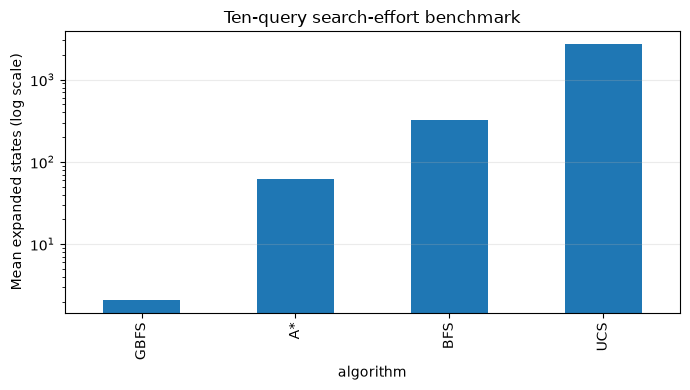
\includegraphics[width=.88\linewidth,height=5cm,keepaspectratio]{labs/visuals/03-notebook-reference.png}
\end{labvisual}
\begin{refoutput}
\begin{lstlisting}[style=utpterminal]
Saved: ['benchmark.csv', 'benchmark_expansions.png', 'benchmark_summary.csv']
Terminal command (from all_experiments):  python -m pytest utils -q
\end{lstlisting}
\end{refoutput}

\textbf{Read the result.} Regenerate this plot rather than copying it. The vertical axis is logarithmic, so the gap between A$^\star$ and UCS is much larger than it looks.
\end{labanswer}

\begin{yourturn}
\begin{enumerate}
  \item \textbf{Add two tests.} Append the two tests below to \texttt{utils/test\_search.py}, then rerun \texttt{python -m pytest utils -q}. The first checks a boundary case for the informed searches. The second pins down what happens when two routes cost the same. Check the result contract, not only the \texttt{found} flag.
  \item \textbf{Use the command line.} Run \texttt{ucs}, \texttt{gbfs} and \texttt{astar} from \texttt{DOH} to \texttt{LIM}. Record cost, route and expansions for each.
  \item \textbf{Find the boundary.} Open \texttt{demo\_robot\_maze.py} and answer: which function plays the role that \texttt{openflights.py} plays for airports, and which lines of \texttt{core.py} had to change for the maze to work?
\end{enumerate}
\begin{lstlisting}[style=utppython]
def test_start_equals_goal_informed():
    h = {"A": 0.0}.get
    for algorithm in (gbfs, astar):
        result = algorithm({"A": []}, "A", "A", h)
        assert result.found and result.path == ["A"]
        assert result.hops == 0 and result.path_cost_km == 0


def test_equal_cost_routes_keep_the_minimum_cost():
    graph = {"S": [("A", 1.0), ("B", 1.0)], "A": [("G", 1.0)], "B": [("G", 1.0)], "G": []}
    assert ucs(graph, "S", "G").path_cost_km == pytest.approx(2.0)
\end{lstlisting}
\end{yourturn}

\begin{expectedfindings}
\begin{enumerate}
  \item \texttt{10 passed}. Question~3's reference output will now read 10 instead of 8, which is correct. If you remove the tests again, it returns to 8.
  \item UCS: 14,856~km via MAD, 3,046 expanded. GBFS: 15,333~km via GRU, 2 expanded. A$^\star$: 14,856~km via MAD, 112 expanded.
  \item \texttt{build\_graph} is the maze's loader, and no line of \texttt{core.py} changed. That is the domain boundary of \figref{fig:domains}: a new domain needs a new loader and nothing else.
\end{enumerate}
\end{expectedfindings}

\begin{troubleshoot}
\begin{description}
  \item[\texttt{No module named pytest}] Your environment is not active, or the requirements were not installed in it. Activate it and run \texttt{pip install -r requirements.txt}.
  \item[\texttt{No module named utils}] Run \texttt{python -m utils} and \texttt{python -m pytest utils} from inside \texttt{all\_experiments/}.
  \item[A test fails after you edited \texttt{core.py}] Good: that is what the tests are for. Read which test failed; each one names one way a search can break.
\end{description}
\end{troubleshoot}

\begin{verification}
\begin{itemize}
  \item All five algorithms return a \texttt{SearchResult} with identical fields.
  \item All tests pass with \texttt{python -m pytest utils -q}, without any dataset.
  \item The command line prints the KUL$\to$HKT$\to$LED$\to$HEL$\to$KEF route and 11,461~km, as Lab~2 found.
  \item Every algorithm succeeds on all ten benchmark queries, and A$^\star$ matches the UCS cost on each.
  \item \texttt{results/lab03/} holds \texttt{benchmark.csv}, \texttt{benchmark\_summary.csv} and \texttt{benchmark\_expansions.png}.
\end{itemize}
\end{verification}

\begin{labdeliverable}
\begin{itemize}
  \item Restart the kernel and run all cells without errors.
  \item Submit the executed notebook, your edited \texttt{test\_search.py} and the generated \texttt{results/lab03/} folder.
  \item Add a short conclusion: recommend a default method for distance-based routing, and explain which module would change for a different graph domain.
\end{itemize}
\end{labdeliverable}


\labsection{3}{Search Engineering: Package, Tests, CLI, and Benchmark}{sec:lab03-search-code}

\begin{labproject}{Turn Labs 1--2 into a reproducible Python toolkit}
\textbf{Read first.} Chapter~\ref{ch:searchpatterns}.\\
\textbf{Goal.} Standardise five algorithms, verify them with dataset-free tests, expose a command-line interface, and benchmark ten route queries.\\
\textbf{Scenario.} Convert notebook logic into reusable, testable software.\\
\textbf{Data.} The OpenFlights files and \texttt{all\_experiments/utils/search\_queries.csv}; unit tests use hand-made graphs.\\
\textbf{Notebook.} \texttt{all\_experiments/lab03\_search\_engineering\_worked.ipynb}; implementation and tests are in \texttt{all\_experiments/utils/}.\\
\textbf{Hand in.} The executed notebook, the \texttt{results/lab03/} folder and a short conclusion, as listed in the checklist at the end of this sheet.
\end{labproject}

\begin{labmode}
\begin{enumerate}
  \item Activate your course environment.
  \item From \texttt{all\_experiments/}, run the tests and one route search in a terminal. These two commands should work before you open the notebook.
  \item Start Jupyter from the same folder, open the notebook, and choose \textbf{Restart Kernel and Run All Cells}. Everything runs in a few seconds.
\end{enumerate}
\begin{lstlisting}[style=utpterminal]
cd all_experiments
python -m pytest utils -q
python -m utils --algorithm astar --start KUL --goal KEF
jupyter lab
\end{lstlisting}
Prefer a plain script? From the course folder, \texttt{python all\_experiments/lab03\_search\_engineering\_worked.py} runs the same code and writes the same evidence.
\end{labmode}

\courselabflow{Define API}{Test tiny graphs}{Run CLI}{Benchmark routes}


\labroutine

\begin{yourturn}
\textbf{Warm-up on paper.} The notebook's tiny graph is below. Before running anything, write down the path and cost you expect from each of BFS, DFS, UCS, GBFS and A$^\star$. The heuristic is $h(S)=5$, $h(A)=4$, $h(B)=1$, $h(G)=0$.
\begin{lstlisting}[style=utppython]
toy = {"S": [("A", 2.0), ("B", 5.0)], "A": [("G", 5.0)], "B": [("G", 1.0)], "G": []}
\end{lstlisting}
\end{yourturn}

\textbf{Setup.} Run the imports and path setup first, and keep this kernel state for the later questions. In the script version the first seven lines also set the working directory.
\lstinputlisting[style=utppython,firstline=1,lastline=7]{all_experiments/lab03_search_engineering_worked.py}
\lstinputlisting[style=utppython,firstline=8,lastline=23]{all_experiments/lab03_search_engineering_worked.py}

\textbf{Read the shared search engine.} Labs~1 and~2 used this module without looking inside. Read it now, in five parts, before running the engineering checks. It lives at \texttt{all\_experiments/utils/core.py}, and the package initialiser exposes these functions to every notebook.

\noindent\textbf{Result record and path reconstruction.}
\lstinputlisting[style=utppython,firstline=1,lastline=42]{all_experiments/utils/core.py}
\noindent\textbf{Cost accounting and BFS.}
\lstinputlisting[style=utppython,firstline=43,lastline=74]{all_experiments/utils/core.py}
\noindent\textbf{DFS and the priority-frontier interface.}
\lstinputlisting[style=utppython,firstline=75,lastline=106]{all_experiments/utils/core.py}
\noindent\textbf{Priority search, stale entries and termination.}
\lstinputlisting[style=utppython,firstline=107,lastline=135]{all_experiments/utils/core.py}
\noindent\textbf{UCS, greedy and A$^\star$ entry points.}
\lstinputlisting[style=utppython,firstline=136,lastline=148]{all_experiments/utils/core.py}

\begin{labquestion}{1}{Standardise the interface}
Every algorithm must return the same fields. Show the fields of \texttt{SearchResult}, then run all five algorithms on the small hand-made graph and display the results as one table.
\end{labquestion}
\begin{labanswer}
\courselabtrace{Keep responsibilities separate}{Loader}{CSV rows become a weighted graph}{Search}{Graph and endpoints become SearchResult}{Reporter}{Result becomes a table or route plot}

Use this fixture before the airline benchmark. A hop-minimising algorithm can choose either two-hop route according to its neighbour order, because it does not look at their weights.
\courselabtrace{Trace the actual search-engineering fixture}{1. Input / state}{toy has S to A cost 2, S to B cost 5, A to G cost 5, and B to G cost 1.}{2. Operation}{Routes S-A-G and S-B-G both have two hops; their costs are 7 and 6.}{3. Check}{UCS selects cost 6. With the supplied consistent h, A-star must also return cost 6.}


\lstinputlisting[style=utppython,firstline=25,lastline=39]{all_experiments/lab03_search_engineering_worked.py}
\begin{refoutput}
\begin{lstlisting}[style=utpterminal]
SearchResult fields: ['found', 'path', 'hops', 'path_cost_km', 'expanded', 'max_frontier', 'runtime_ms']
      path          hops  cost  expanded  max_frontier
BFS   S -> A -> G      2   7.0         3             2
DFS   S -> A -> G      2   7.0         2             2
UCS   S -> B -> G      2   6.0         3             2
GBFS  S -> B -> G      2   6.0         2             2
A*    S -> B -> G      2   6.0         3             2
\end{lstlisting}
\end{refoutput}

\textbf{What it means.} All five functions return a \texttt{SearchResult} with identical fields, so one loop can benchmark them. BFS and DFS return the two-edge route through A at cost 7, while UCS and A$^\star$ return the cheaper route through B at cost 6. GBFS also picks B, because $h(B) < h(A)$.
\end{labanswer}

\begin{labquestion}{2}{Separate responsibilities}
Search logic, data loading, plotting and the command line must live in separate modules. List the package's modules with their one-line purpose, and the names it exports.
\end{labquestion}
\begin{labanswer}
\lstinputlisting[style=utppython,firstline=41,lastline=45]{all_experiments/lab03_search_engineering_worked.py}
\begin{refoutput}
\begin{lstlisting}[style=utpterminal]
__init__.py      Helper code for the AI course notebooks.
__main__.py      Command-line route search (Lab 3).
core.py          Graph-search algorithms shared by Labs 1-3: BFS, DFS, UCS, GBFS and A*.
openflights.py   Load the OpenFlights airport and route files into a weighted graph.
plotting.py      Plot airport routes on longitude/latitude axes (Labs 1-3).
test_search.py   Unit tests for utils.core on tiny hand-made graphs (no dataset needed).

Exported names: SearchResult, astar, best_first, bfs, dfs, gbfs, ucs, haversine_km, load_openflights, route_is_valid, plot_route_paths
\end{lstlisting}
\end{refoutput}

\textbf{What it means.} \texttt{core.py} holds the five algorithms and knows nothing about airports; \texttt{openflights.py} cleans the CSV files and computes distances; \texttt{plotting.py} draws routes; \texttt{\_\_main\_\_.py} is the command line; \texttt{test\_search.py} holds the tests. Each module can be changed and tested on its own.
\end{labanswer}

\textbf{Connect it to the chapter.} The module split is the same boundary as this picture: everything above the frontier policy belongs to the problem, and the policy names the algorithm.
% Reused from chapters/03-search-implementation-patterns.tex
\begin{labvisual}{Recall the chapter model}
\begin{labgraphic}
\begin{tikzpicture}[
  box/.style={draw=UTPBlue,fill=UTPPaleBlue,rounded corners=2mm,minimum width=2.7cm,minimum height=0.9cm,align=center,font=\small\bfseries\color{UTPNavy}},
  policy/.style={draw=UTPOrange!70!black,fill=UTPPaleOrange,rounded corners=1.5mm,minimum width=1.55cm,minimum height=0.65cm,align=center,font=\scriptsize\bfseries\color{UTPOrange!85!black}},
  arr/.style={-{Stealth[length=2mm]},thick,draw=UTPTeal}
]
\node[box] (state) {State\\representation};
\node[box,right=0.7cm of state] (succ) {Successor\\function};
\node[box,right=0.7cm of succ] (frontier) {Frontier\\policy};
\node[box,right=0.7cm of frontier] (result) {Goal test\\and result};
\draw[arr] (state)--(succ);
\draw[arr] (succ)--(frontier);
\draw[arr] (frontier)--(result);
\node[policy,below=0.75cm of frontier,xshift=-3.2cm] (bfs) {BFS: depth};
\node[policy,right=0.18cm of bfs] (dfs) {DFS: recency};
\node[policy,right=0.18cm of dfs] (ucs) {UCS: $g$};
\node[policy,right=0.18cm of ucs] (gbfs) {GBFS: $h$};
\node[policy,right=0.18cm of gbfs] (astar) {A*: $g+h$};
\draw[arr] (ucs.north) -- (frontier.south);
\node[font=\scriptsize\color{UTPMuted}] at (0.55,-2.35) {swap one line $\rightarrow$ different algorithm};
\end{tikzpicture}
\end{labgraphic}\end{labvisual}


\begin{labquestion}{3}{Run the automated tests}
The tests use tiny hand-made graphs and cover start = goal, unreachable goal, cycles, different objectives, frontier updates, consistent A$^\star$, non-optimal GBFS and negative costs. Run them with pytest from inside the notebook.
\end{labquestion}
\begin{labanswer}
\lstinputlisting[style=utppython,firstline=47,lastline=49]{all_experiments/lab03_search_engineering_worked.py}
\begin{refoutput}
\begin{lstlisting}[style=utpterminal]
........                                                                 [100%]
8 passed in 0.71s
\end{lstlisting}
\end{refoutput}

\textbf{What it means.} All eight tests pass in under a second. They need no dataset, so they run anywhere, including on a continuous-integration server. A harmless \texttt{PytestCacheWarning} may also appear if the folder is read-only or synced by a cloud drive.
\end{labanswer}

\begin{labquestion}{4}{Exercise the command-line interface}
Run \texttt{python -m utils --algorithm astar --start KUL --goal KEF} as a subprocess and show its output.
\end{labquestion}
\begin{labanswer}
\lstinputlisting[style=utppython,firstline=51,lastline=54]{all_experiments/lab03_search_engineering_worked.py}
\begin{refoutput}
\begin{lstlisting}[style=utpterminal]
ASTAR: found=True, hops=4, cost_km=11461.3, expanded=69, runtime_ms=3.75
KUL -> HKT -> LED -> HEL -> KEF
\end{lstlisting}
\end{refoutput}

\textbf{What it means.} The command line prints the same route and 11,461~km that Lab~2 found, because the notebook and the terminal share one implementation.
\end{labanswer}

\begin{labquestion}{5}{Benchmark ten route pairs}
Run BFS, UCS, GBFS and A$^\star$ on the ten queries in \texttt{utils/search\_queries.csv} and summarise success rate, mean cost, mean hops, expanded nodes and runtime per algorithm. Save \texttt{benchmark.csv} and \texttt{benchmark\_summary.csv}.
\end{labquestion}
\begin{labanswer}
\lstinputlisting[style=utppython,firstline=56,lastline=83]{all_experiments/lab03_search_engineering_worked.py}
\begin{refoutput}
\begin{lstlisting}[style=utpterminal]
A* cost equals UCS on all 10 queries: True
GBFS is costlier than UCS on 7 of 10 queries
\end{lstlisting}
\end{refoutput}

\textbf{What it means.} Every algorithm succeeds on all ten queries. A$^\star$ matches the UCS cost on every query with a fraction of the expansions; BFS has the highest mean cost because it optimises hops; GBFS expands the fewest states but returns a costlier route on seven queries. For distance-based routing, A$^\star$ is the best default among the exact methods.
\end{labanswer}

\begin{labquestion}{6}{Save the evidence}
Save a bar chart of mean expansions per algorithm. Then note the one-line terminal command that runs the same tests outside the notebook.
\end{labquestion}
\begin{labanswer}
\lstinputlisting[style=utppython,firstline=85,lastline=91]{all_experiments/lab03_search_engineering_worked.py}
\begin{labvisual}{Reference plot from the supplied notebook}
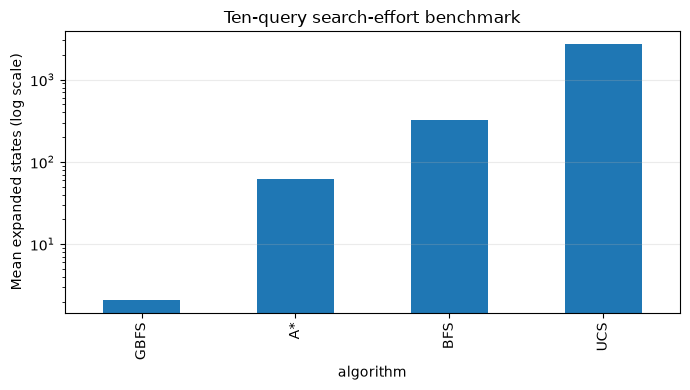
\includegraphics[width=.88\linewidth,height=5cm,keepaspectratio]{labs/visuals/03-notebook-reference.png}
\end{labvisual}
\begin{refoutput}
\begin{lstlisting}[style=utpterminal]
Saved: ['benchmark.csv', 'benchmark_expansions.png', 'benchmark_summary.csv']
Terminal command (from all_experiments):  python -m pytest utils -q
\end{lstlisting}
\end{refoutput}

\textbf{Read the result.} Regenerate this plot rather than copying it. The vertical axis is logarithmic, so the gap between A$^\star$ and UCS is much larger than it looks.
\end{labanswer}

\begin{yourturn}
\begin{enumerate}
  \item \textbf{Add two tests.} Append the two tests below to \texttt{utils/test\_search.py}, then rerun \texttt{python -m pytest utils -q}. The first checks a boundary case for the informed searches. The second pins down what happens when two routes cost the same. Check the result contract, not only the \texttt{found} flag.
  \item \textbf{Use the command line.} Run \texttt{ucs}, \texttt{gbfs} and \texttt{astar} from \texttt{DOH} to \texttt{LIM}. Record cost, route and expansions for each.
  \item \textbf{Find the boundary.} Open \texttt{demo\_robot\_maze.py} and answer: which function plays the role that \texttt{openflights.py} plays for airports, and which lines of \texttt{core.py} had to change for the maze to work?
\end{enumerate}
\begin{lstlisting}[style=utppython]
def test_start_equals_goal_informed():
    h = {"A": 0.0}.get
    for algorithm in (gbfs, astar):
        result = algorithm({"A": []}, "A", "A", h)
        assert result.found and result.path == ["A"]
        assert result.hops == 0 and result.path_cost_km == 0


def test_equal_cost_routes_keep_the_minimum_cost():
    graph = {"S": [("A", 1.0), ("B", 1.0)], "A": [("G", 1.0)], "B": [("G", 1.0)], "G": []}
    assert ucs(graph, "S", "G").path_cost_km == pytest.approx(2.0)
\end{lstlisting}
\end{yourturn}

\begin{expectedfindings}
\begin{enumerate}
  \item \texttt{10 passed}. Question~3's reference output will now read 10 instead of 8, which is correct. If you remove the tests again, it returns to 8.
  \item UCS: 14,856~km via MAD, 3,046 expanded. GBFS: 15,333~km via GRU, 2 expanded. A$^\star$: 14,856~km via MAD, 112 expanded.
  \item \texttt{build\_graph} is the maze's loader, and no line of \texttt{core.py} changed. That is the domain boundary of \figref{fig:domains}: a new domain needs a new loader and nothing else.
\end{enumerate}
\end{expectedfindings}

\begin{troubleshoot}
\begin{description}
  \item[\texttt{No module named pytest}] Your environment is not active, or the requirements were not installed in it. Activate it and run \texttt{pip install -r requirements.txt}.
  \item[\texttt{No module named utils}] Run \texttt{python -m utils} and \texttt{python -m pytest utils} from inside \texttt{all\_experiments/}.
  \item[A test fails after you edited \texttt{core.py}] Good: that is what the tests are for. Read which test failed; each one names one way a search can break.
\end{description}
\end{troubleshoot}

\begin{verification}
\begin{itemize}
  \item All five algorithms return a \texttt{SearchResult} with identical fields.
  \item All tests pass with \texttt{python -m pytest utils -q}, without any dataset.
  \item The command line prints the KUL$\to$HKT$\to$LED$\to$HEL$\to$KEF route and 11,461~km, as Lab~2 found.
  \item Every algorithm succeeds on all ten benchmark queries, and A$^\star$ matches the UCS cost on each.
  \item \texttt{results/lab03/} holds \texttt{benchmark.csv}, \texttt{benchmark\_summary.csv} and \texttt{benchmark\_expansions.png}.
\end{itemize}
\end{verification}

\begin{labdeliverable}
\begin{itemize}
  \item Restart the kernel and run all cells without errors.
  \item Submit the executed notebook, your edited \texttt{test\_search.py} and the generated \texttt{results/lab03/} folder.
  \item Add a short conclusion: recommend a default method for distance-based routing, and explain which module would change for a different graph domain.
\end{itemize}
\end{labdeliverable}


\part{Approximate Reasoning and Intelligent Control}
\chapter{Fuzzy Logic and ANFIS}
\label{ch:fuzzy}

\chapterguide%
  {Know Boolean true/false logic and be comfortable with NumPy arrays and a scikit-learn train/test split.}
  {express a graded concept as a membership function; trace the four stages of a fuzzy inference system on one reading; distinguish Mamdani from Sugeno rules; explain what ANFIS learns and how; and evaluate a learned model without leaking test data into its selection.}

Search needs exact facts: a cell is either a wall or it is not. Much of what we know about the world is not like that. Is $29^\circ$C hot? Is 55\,\% humidity uncomfortable? People handle such questions easily, with rules of thumb full of vague words, and this chapter shows how to make those rules run on a computer.

Lab~4 uses one air-quality dataset for two tasks. A hand-written \term{fuzzy controller} maps temperature and humidity to ventilation demand. An \term{ANFIS} regressor predicts carbon monoxide from two gas sensors, fitting its rule parameters to about 5,000 measurements. We examine the controller first, then the learner.

\section{From crisp truth to fuzzy membership}

Classical logic has two answers, true and false. Fuzzy logic allows a \term{degree of membership} $0\le\mu(x)\le1$. Suppose a ventilation fan follows the rule ``if it is hot, run at full speed'' and ``hot'' means above $30^\circ$C. At $29.9^\circ$C the fan is idle, and at $30.1^\circ$C it is at full speed. A change you could not feel on your skin flips the whole system.

\begin{analogy}
An ordinary light switch is either off or on. A dimmer sweeps smoothly from dark to full brightness and cannot go past either end. Crisp logic is the switch. Fuzzy logic is the dimmer: ``hot'' can be 0.47 on, and the fan responds in proportion.
\end{analogy}

\begin{utpfig}[Crisp versus fuzzy membership]{``Hot'' as a crisp set and as a fuzzy set, the second using the set from Lab~4. The crisp version forces a decision at one point. The fuzzy version reports a degree, so $35^\circ$C is hot to degree $0.47$.}{fig:crisp-fuzzy}
\begin{tikzpicture}
\begin{axis}[
  name=crisp, width=6.6cm, height=4.2cm,
  xlabel={temperature ($^\circ$C)}, ylabel={$\mu(x)$},
  title={Crisp set: ``hot''},
  xmin=0, xmax=50, ymin=-0.08, ymax=1.18,
  ytick={0,0.5,1}, xtick={0,10,20,30,40,50},
  axis lines=left, grid=major, grid style={draw=UTPPaleBlue}]
\addplot[UTPRed,thick] coordinates {(0,0) (30,0)};
\addplot[UTPRed,thick] coordinates {(30,1) (50,1)};
\addplot[UTPRed,dashed,thin] coordinates {(30,0) (30,1)};
\addplot[only marks,mark=*,UTPRed,mark size=1.4pt] coordinates {(30,1)};
\addplot[only marks,mark=o,UTPRed,mark size=1.4pt] coordinates {(30,0)};
\end{axis}
\begin{axis}[
  at={(crisp.right of south east)}, xshift=1.15cm, anchor=left of south west,
  width=6.6cm, height=4.2cm,
  xlabel={temperature ($^\circ$C)}, ylabel={$\mu(x)$},
  title={Fuzzy set: ``hot''},
  xmin=0, xmax=50, ymin=-0.08, ymax=1.18,
  ytick={0,0.5,1}, xtick={0,10,20,26,35,45},
  axis lines=left, grid=major, grid style={draw=UTPPaleBlue}]
\addplot[UTPGreen,thick] coordinates {(0,0) (26,0) (45,1) (50,1)};
\addplot[UTPOrange,dashed,thin] coordinates {(35,0) (35,0.47)};
\addplot[UTPOrange,dashed,thin] coordinates {(0,0.47) (35,0.47)};
\addplot[only marks,mark=*,UTPOrange,mark size=1.6pt] coordinates {(35,0.47)};
\node[font=\scriptsize\color{UTPOrange},anchor=west] at (axis cs:36,0.36) {$\mu(35)=0.47$};
\end{axis}
\end{tikzpicture}
\end{utpfig}

\begin{pitfall}
A membership of 0.47 is not a 47\,\% chance that it is hot. The temperature is known exactly, and nothing about it is uncertain. The word ``hot'' is what has edges that fade. Fuzzy logic models vague words; probability models unknown facts.
\end{pitfall}

\begin{intuition}
Fuzzy logic attaches numbers to graded words such as ``cold'', ``humid'' and ``fast'', which makes verbal rules executable. You already adjust a shower this way: nobody solves an equation, you just think ``a bit too cold, so a little hotter''.
\end{intuition}

\section{Membership functions}

A \term{membership function} maps a crisp value to a degree. The lab uses triangles, the simplest shape that rises to 1 and falls back to 0, defined by three points $a\le b\le c$:
\[
\mu(x)=\max\!\Big(0,\;\min\!\Big(\frac{x-a}{b-a},\;\frac{c-x}{c-b}\Big)\Big).
\]
The outer sets are \term{shoulders}: $a=b$ gives membership~1 below the peak, and $b=c$ gives membership~1 above it, so extreme readings still activate rules. The temperature sets are cold $(0,0,18)$, mild $(12,22,32)$ and hot $(26,45,45)$ (\figref{fig:membership}). They overlap on purpose. At $15^\circ$C the reading is partly cold and partly mild at the same time, and that overlap is what makes the output change smoothly.

\begin{utpfig}[The lab's temperature memberships]{Cold and hot are shoulders; mild is triangular. At $15^\circ$C, cold membership is $(18-15)/18=0.17$ and mild membership is $(15-12)/10=0.30$, so rules for both will fire.}{fig:membership}
\begin{tikzpicture}
\begin{axis}[
  width=0.88\linewidth, height=5.6cm,
  xmin=0, xmax=45, ymin=0, ymax=1.08,
  xlabel={Temperature ($^\circ$C)}, ylabel={Membership},
  xtick={0,12,15,18,22,26,32,45}, ytick={0,0.17,0.3,0.5,1},
  yticklabels={0,0.17,0.30,0.5,1},
  legend columns=3, legend style={at={(0.5,-0.26)},anchor=north},
  clip=false]
\addplot[draw=UTPBlue,very thick] coordinates {(0,1) (18,0) (45,0)};
\addlegendentry{cold $(0,0,18)$}
\addplot[draw=UTPTeal,very thick] coordinates {(0,0) (12,0) (22,1) (32,0) (45,0)};
\addlegendentry{mild $(12,22,32)$}
\addplot[draw=UTPOrange,very thick] coordinates {(0,0) (26,0) (45,1)};
\addlegendentry{hot $(26,45,45)$}
\addplot[draw=UTPRed,dashed,thick] coordinates {(15,0) (15,1.02)};
\addplot[only marks,mark=*,mark size=2.2pt,UTPBlue] coordinates {(15,0.167)};
\addplot[only marks,mark=*,mark size=2.2pt,UTPTeal] coordinates {(15,0.3)};
\node[font=\scriptsize\color{UTPBlue},anchor=west] at (axis cs:15.6,0.12) {$\mu_{\text{cold}}(15)=0.17$};
\node[font=\scriptsize\color{UTPTeal},anchor=west] at (axis cs:15.6,0.36) {$\mu_{\text{mild}}(15)=0.30$};
\end{axis}
\end{tikzpicture}
\end{utpfig}

The lab implements the triangle in a few lines, with the shoulder cases written out explicitly:

\lstinputlisting[style=utppython,firstline=38,lastline=43]{all_experiments/lab04_fuzzy_anfis_worked.py}

\begin{pitfall}
A \texttt{trimf} that assumes $a<b<c$ divides by zero for shoulders or returns incorrect zero memberships. This can disable the ``cold'' and ``dry'' rules, leaving only a fallback output. Question~3 of the lab catches this by checking five points with known answers.
\end{pitfall}

\section{The four stages of a fuzzy inference system}

A \term{fuzzy inference system} (FIS) turns crisp inputs into a crisp output by passing through words in between (\figref{fig:fis-pipeline}). The numbers go in, become degrees of ``cold'' and ``comfortable'', meet the rules, and come back out as one number for the fan.

\begin{utpfig}[The four stages of a fuzzy inference system]{Inputs of $15^\circ$C and 45\,\% become membership degrees, activate rules and yield one crisp ventilation demand.}{fig:fis-pipeline}
\begin{tikzpicture}[font=\small]
\node[utpbox,minimum width=1.65cm,minimum height=0.9cm,fill=UTPPaleGray,draw=UTPMuted,
      font=\scriptsize\color{UTPNavy}] (in) at (0,0) {crisp in\\\textbf{$15^\circ$C, 45\,\%}};
\node[utpbox,minimum width=2.25cm,minimum height=0.9cm,font=\scriptsize\color{UTPNavy}]
  (fz) at (2.5,0) {\textbf{Fuzzification}\\$\to$ degrees};
\node[utpbox,minimum width=2.25cm,minimum height=0.9cm,font=\scriptsize\color{UTPNavy}]
  (rb) at (5.2,0) {\textbf{Rule base}\\IF--THEN};
\node[utpbox,minimum width=2.25cm,minimum height=0.9cm,font=\scriptsize\color{UTPNavy}]
  (ie) at (7.9,0) {\textbf{Inference}\\combine rules};
\node[utpbox,minimum width=2.25cm,minimum height=0.9cm,font=\scriptsize\color{UTPNavy}]
  (df) at (10.6,0) {\textbf{Defuzzification}\\$\to$ one number};
\node[utpbox,minimum width=1.55cm,minimum height=0.9cm,fill=UTPPaleTeal,draw=UTPGreen,
      font=\scriptsize\color{UTPNavy}] (out) at (13.0,0) {crisp out\\\textbf{40.4\,\%}};
\foreach \a/\b in {in/fz, fz/rb, rb/ie, ie/df, df/out}{\draw[utparrow] (\a)--(\b);}
\node[utplabel,anchor=north,align=center,color=UTPOrange] at (2.5,-0.6)
  {cold $0.17$, mild $0.30$\\comfortable $0.75$};
\node[utplabel,anchor=north,align=center,color=UTPOrange] at (5.2,-0.6)
  {low fires $0.17$\\medium fires $0.30$};
\node[utplabel,anchor=north,align=center,color=UTPOrange] at (7.9,-0.6)
  {clipped sets\\joined by max};
\node[utplabel,anchor=north,align=center,color=UTPOrange] at (10.6,-0.6)
  {centroid of\\that shape};
\draw[utpbrace] (1.4,0.68) -- (11.8,0.68);
\node[utplabel,anchor=south,color=UTPNavy] at (6.6,1.0)
  {everything inside this brace is fuzzy; the two ends are not};
\end{tikzpicture}
\end{utpfig}

\begin{utptable}
\begin{tabularx}{\linewidth}{@{}>{\bfseries\leavevmode\color{UTPNavy}}m{0.20\linewidth}X@{}}
\toprule
\rowcolor{UTPPaleBlue!92}
\utpth{Stage} & \utpth{What happens, and where it is in the lab code} \\
\midrule
Fuzzification & Each crisp input is turned into one degree per set: \texttt{degree(T\_range, mf, temperature)} for every set. \\
Rule base & IF--THEN rules over the set names. AND is \texttt{min}; rules with the same conclusion are joined with \texttt{max}. \\
Inference & Each output set is clipped at its rule's strength; the clipped sets are joined with \texttt{np.maximum.reduce}. \\
Defuzzification & The centroid of the joined shape: $\sum x\,\mu(x)\,/\,\sum\mu(x)$ over the output range. \\
\bottomrule
\end{tabularx}
\end{utptable}

\subsection{The rule base}

The controller has six rules, written so that heat or humidity raises the demand and cool, dry conditions lower it:

\begin{utptable}
\begin{tabularx}{\linewidth}{@{}>{\bfseries\leavevmode\color{UTPNavy}}m{0.12\linewidth}X@{}}
\toprule
\rowcolor{UTPPaleBlue!92}
\utpth{Output} & \utpth{Fires when} \\
\midrule
low & cold AND dry, \quad or \quad cold AND comfortable \\
medium & mild AND dry, \quad or \quad mild AND comfortable, \quad or \quad cold AND humid \\
high & hot, \quad or \quad humid \\
\bottomrule
\end{tabularx}
\end{utptable}

In code the three outputs take three lines:

\lstinputlisting[style=utppython,firstline=60,lastline=63]{all_experiments/lab04_fuzzy_anfis_worked.py}

Two small choices make this work. AND takes the \texttt{min}, because a chain is only as strong as its weakest link: ``cold AND comfortable'' cannot be truer than its less true part. Alternatives take the \texttt{max}, because a conclusion with several possible reasons is as well supported as its best reason.

\subsection{Defuzzification by centroid}

The rules produce a fuzzy output set, but the fan needs a number. At $15^\circ$C and 45\,\%, clip the ``low'' output set at $0.17$ and the ``medium'' set at $0.30$, combine them, and report the centroid (\figref{fig:defuzz}). If you cut that shape out of cardboard, the centroid is the point where it would balance on a fingertip. A stronger rule adds weight to its side and pulls the balance point towards it.

\begin{utpfig}[Defuzzification by centroid]{Defuzzifying the $15^\circ$C, 45\,\% reading. Low is clipped at $0.17$ and medium at $0.30$; high does not fire. The centre of area of their union is $40.4\,\%$. A stronger medium rule would pull the centroid to the right.}{fig:defuzz}
\begin{tikzpicture}
\begin{axis}[
  width=0.82\linewidth, height=5.4cm,
  xmin=0, xmax=100, ymin=0, ymax=1.12,
  xlabel={Ventilation demand (\%)}, ylabel={Membership},
  xtick={0,25,40.4,50,75,100}, xticklabels={0,25,40.4,50,75,100},
  ytick={0,0.17,0.3,0.6,1}, yticklabels={0,0.17,0.30,0.6,1},
  axis lines=left, grid=major, grid style={draw=UTPPaleBlue},
  clip=false]
\addplot[draw=UTPMuted!45,thin] coordinates {(0,1) (45,0)};
\addplot[draw=UTPMuted!45,thin] coordinates {(25,0) (50,1) (75,0)};
\addplot[draw=UTPMuted!45,thin] coordinates {(55,0) (100,1)};
\addplot[draw=UTPTeal,very thick,fill=UTPPaleTeal,fill opacity=0.75]
  coordinates {(0,0) (0,0.167) (29.2,0.167) (32.5,0.3) (67.5,0.3) (75,0) (0,0)};
\addplot[UTPRed,dashed,thick] coordinates {(40.4,0) (40.4,0.62)};
\addplot[only marks,mark=*,mark size=2.4pt,UTPRed] coordinates {(40.4,0.3)};
\node[font=\scriptsize\color{UTPRed},anchor=south] at (axis cs:40.4,0.65) {centroid $=40.4$};
\node[font=\scriptsize\color{UTPBlue},anchor=west] at (axis cs:2,0.25) {low clipped at $0.17$};
\node[font=\scriptsize\color{UTPTeal},anchor=west] at (axis cs:44,0.38) {medium clipped at $0.30$};
\node[font=\scriptsize\color{UTPMuted},anchor=west] at (axis cs:78,0.5) {high: not fired};
\end{axis}
\end{tikzpicture}
\end{utpfig}

\begin{workedexample}
At $15^\circ$C and 45\,\% relative humidity the memberships are cold $0.17$, mild $0.30$, comfortable $(45-30)/20=0.75$, and all others~$0$. The rule strengths follow:
\[
\text{low}=\min(0.17,0.75)=0.17,\qquad
\text{medium}=\min(0.30,0.75)=0.30,\qquad
\text{high}=0.
\]
Clipping the low and medium output sets at those strengths and taking the centroid of their union gives a ventilation demand of $40.4\,\%$: a little below ``medium'', pulled down by the cold rule.
\end{workedexample}

\begin{tryit}
Trace $28^\circ$C and 45\,\% by hand before reading on. Which temperature sets are non-zero, which rules fire, and with what strength? Then run \texttt{ventilation(28, 45)} in the Lab~4 notebook.

\emph{Answer.} Mild is $(32-28)/10=0.40$ and hot is $(28-26)/19=0.11$; comfortable is still $0.75$. So low $=0$, medium $=\min(0.40,0.75)=0.40$ and high $=0.11$. The output set now has weight on the high side, and the code returns $55.5\,\%$.
\end{tryit}

\section{Validating a controller}

Check the controller against expectations written down \emph{before} viewing its output. Lab~4 uses two checks:

\begin{description}
  \item[Fixed points.] Five operating conditions with a qualitative expected answer: $(10^\circ, 30\,\%)$ should be low, $(20^\circ, 50\,\%)$ medium, and $(35^\circ, 50\,\%)$, $(25^\circ, 80\,\%)$ and $(40^\circ, 80\,\%)$ high. The controller returns 18.9, 50.0, 82.3, 83.8 and 84.2\,\%. Each lands in its band.
  \item[The control surface.] Plot the output over a temperature--humidity grid. It should rise towards hot, humid conditions without cliffs or unexplained plateaus, which can reveal membership gaps or inactive rules.
\end{description}

A surface also exposes gaps in coverage. Every reading must fire at least one rule. If you delete ``humid'' from the \texttt{high} rule, then at $(25^\circ, 80\,\%)$ no rule fires, the output set is empty, and the centroid becomes a division by zero. That happens on 99 of the 1,886 grid points. The full rule base has no such gap.

\begin{keyidea}
Check known inputs and the full control surface. One plausible output can hide inactive rules.
\end{keyidea}

\section{Mamdani and Sugeno systems}

The controller above is a \term{Mamdani} system: each rule outputs a fuzzy \emph{set}, and those sets are combined and defuzzified. A \term{Sugeno} rule instead outputs a formula, such as $0.6\,x_1+0.2\,x_2+1.3$, and the final output is the firing-strength-weighted average of those formulas (\figref{fig:mamdani-sugeno}). One way to picture it: each Sugeno rule is a small straight-line model that is valid in its own neighbourhood, and the memberships decide how much each one gets to say at any given input (\figref{fig:sugeno-blend}).

\begin{utpfig}[Mamdani versus Sugeno rule output]{Mamdani combines fuzzy output sets and defuzzifies them. Sugeno averages numeric rule outputs by firing strength, enabling ANFIS training.}{fig:mamdani-sugeno}
\begin{tikzpicture}[font=\small]
\begin{scope}
\node[font=\bfseries\color{UTPNavy}] at (2.5,2.2) {Mamdani};
\node[utpbox,minimum width=4.6cm,font=\scriptsize\color{UTPNavy}] (r1) at (2.5,1.5)
  {IF sensor is High THEN CO is \textbf{High}};
\node[utplabel,anchor=north,color=UTPOrange] at (2.5,1.05) {\textbf{High} is a fuzzy set};
\begin{scope}[xshift=1.35cm,yshift=-0.55cm,x=0.6cm,y=0.6cm]
\draw[draw=UTPMuted!60,-{Stealth[length=1.6mm]}] (-0.2,0)--(4.0,0);
\draw[draw=UTPMuted!60,-{Stealth[length=1.6mm]}] (0,-0.2)--(0,1.35);
\draw[very thick,draw=UTPOrange] (0.4,0)--(1.8,1.1)--(3.2,0);
\fill[UTPOrange,opacity=0.2] (0.4,0)--(1.8,1.1)--(3.2,0)--cycle;
\end{scope}
\node[utplabel,anchor=north,align=center] at (2.5,-1.35)
  {needs joining, then a centroid};
\end{scope}
\begin{scope}[xshift=7.6cm]
\node[font=\bfseries\color{UTPNavy}] at (2.5,2.2) {Sugeno};
\node[utpbox,minimum width=5.1cm,font=\scriptsize\color{UTPNavy},
      fill=UTPPaleTeal,draw=UTPGreen] (r2) at (2.5,1.5)
  {IF sensor is High THEN CO $=p_0+p_1x_1+p_2x_2$};
\node[utplabel,anchor=north,color=UTPGreen] at (2.5,1.05) {the consequent is a formula};
\node[utpcell,minimum width=3.2cm,minimum height=0.65cm,fill=UTPPaleTeal,draw=UTPGreen,
      font=\scriptsize\bfseries] at (2.5,0.15) {output $=\sum_r \bar w_r\,f_r(x)$};
\node[utplabel,anchor=north,align=center] at (2.5,-1.35)
  {weighted average, no centroid};
\end{scope}
\end{tikzpicture}
\end{utpfig}

\begin{utpfig}[Blending local rules into a curve]{An illustrative one-input Sugeno system with two rules. Bottom: the two memberships say which rule applies where. Top: the two dashed straight lines are the rule outputs, and the solid curve is their weighted average. It follows one line on the left, the other on the right, and bends smoothly between them. Blending straight lines is how ANFIS fits a curved response.}{fig:sugeno-blend}
\begin{tikzpicture}[declare function={
    mone(\x)=exp(-0.5*(\x+1)^2);
    mtwo(\x)=exp(-0.5*(\x-1)^2);
    wone(\x)=mone(\x)/(mone(\x)+mtwo(\x));
    fone(\x)=0.5+0.15*\x;
    ftwo(\x)=-0.6+1.2*\x;
    blend(\x)=wone(\x)*fone(\x)+(1-wone(\x))*ftwo(\x);}]
\begin{axis}[
  name=top, width=0.70\linewidth, height=4.5cm,
  xmin=-3, xmax=3, ymin=-1.2, ymax=3.2,
  xticklabels={}, ylabel={output},
  axis lines=left, grid=major, grid style={draw=UTPPaleBlue},
  domain=-3:3, samples=61]
\addplot[draw=UTPBlue,dashed,thick] {fone(x)};
\addplot[draw=UTPOrange,dashed,thick] {ftwo(x)};
\addplot[draw=UTPGreen,very thick] {blend(x)};
\node[font=\scriptsize\color{UTPBlue},anchor=south west] at (axis cs:-2.9,0.15) {rule 1 output};
\node[font=\scriptsize\color{UTPOrange!85!black},anchor=west] at (axis cs:0.15,-0.8) {rule 2 output};
\node[font=\scriptsize\bfseries\color{UTPGreen},anchor=south east] at (axis cs:2.2,1.95) {blended output};
\end{axis}
\begin{axis}[
  at={(top.south west)}, anchor=north west, yshift=-0.25cm,
  width=0.70\linewidth, height=2.9cm,
  xmin=-3, xmax=3, ymin=0, ymax=1.15,
  xlabel={input $x$}, ylabel={membership}, ytick={0,1},
  axis lines=left, grid=major, grid style={draw=UTPPaleBlue},
  domain=-3:3, samples=61]
\addplot[draw=UTPBlue,thick] {mone(x)};
\addplot[draw=UTPOrange,thick] {mtwo(x)};
\end{axis}
\end{tikzpicture}
\end{utpfig}

\begin{utptable}
\begin{tabularx}{\linewidth}{@{}>{\bfseries\leavevmode\color{UTPNavy}}m{0.15\linewidth}XX@{}}
\toprule
\rowcolor{UTPPaleBlue!92}
\utpth{} & \utpth{Mamdani} & \utpth{Sugeno} \\
\midrule
Rule conclusion & A fuzzy set over the output & A function of the inputs \\
Output & Centroid of the joined, clipped sets & Weighted average of the rule functions \\
Strength & Readable: every conclusion is a word & Trainable: every conclusion is a set of coefficients \\
Used in Lab~4 by & The ventilation controller & ANFIS \\
\bottomrule
\end{tabularx}
\end{utptable}

The Sugeno form is what makes learning possible. Once the firing strengths are fixed, the output is \emph{linear} in the consequent coefficients $p$, so the best coefficients for a training set can be found by ordinary least squares in one step.

\section{ANFIS: a fuzzy system that learns}

Writing rules by hand works when an expert knows the numbers. What if nobody knows exactly where ``high sensor reading'' begins? An \term{Adaptive Neuro-Fuzzy Inference System} (ANFIS) expresses a Sugeno FIS as a five-layer network with learnable parameters (\figref{fig:anfis}). The inference structure stays the same, and data determine the parameters.

\begin{utpfig}[The five layers of an ANFIS network]{ANFIS with two inputs and two memberships each. Layers 1 and 4 contain trainable parameters; layers 2, 3 and 5 perform fixed arithmetic.}{fig:anfis}
\begin{tikzpicture}[font=\small,
  L/.style={circle,draw=UTPBlue,fill=UTPPaleBlue,minimum size=7.5mm,
            font=\scriptsize\color{UTPNavy},inner sep=0.5pt},
  T/.style={circle,draw=UTPOrange,fill=UTPPaleOrange,minimum size=7.5mm,line width=0.9pt,
            font=\scriptsize\color{UTPNavy},inner sep=0.5pt}]
\def\dx{2.45}
\node[utplabel,font=\small\bfseries\color{UTPNavy}] (x) at (-\dx,0.75) {$x_1$};
\node[utplabel,font=\small\bfseries\color{UTPNavy}] (y) at (-\dx,-0.75) {$x_2$};
\node[T] (A1) at (0,1.35) {$A_1$};
\node[T] (A2) at (0,0.45) {$A_2$};
\node[T] (B1) at (0,-0.45) {$B_1$};
\node[T] (B2) at (0,-1.35) {$B_2$};
\node[L] (P1) at (\dx,0.9) {$\Pi$};
\node[L] (P2) at (\dx,-0.9) {$\Pi$};
\node[L] (N1) at (2*\dx,0.9) {$N$};
\node[L] (N2) at (2*\dx,-0.9) {$N$};
\node[T] (C1) at (3*\dx,0.9) {$f_1$};
\node[T] (C2) at (3*\dx,-0.9) {$f_2$};
\node[L] (S) at (4*\dx,0) {$\Sigma$};
\node[utplabel,font=\small\bfseries\color{UTPNavy}] (out) at (4*\dx+1.15,0) {output};
\foreach \t in {A1,A2}{\draw[utpptr] (x)--(\t);}
\foreach \t in {B1,B2}{\draw[utpptr] (y)--(\t);}
\draw[utpptr] (A1)--(P1); \draw[utpptr] (B1)--(P1);
\draw[utpptr] (A2)--(P2); \draw[utpptr] (B2)--(P2);
\draw[utpptr] (P1)--(N1); \draw[utpptr] (P2)--(N2);
\draw[utpptr] (P1)--(N2); \draw[utpptr] (P2)--(N1);
\draw[utpptr] (N1)--(C1); \draw[utpptr] (N2)--(C2);
\draw[utpptr] (C1)--(S);  \draw[utpptr] (C2)--(S);
\draw[utpptr] (S)--(out);
\foreach \i/\lbl in {0/{1. fuzzify}, 1/{2. rule\\strength}, 2/{3. normalise},
                     3/{4. rule\\output}, 4/{5. aggregate}}{
  \node[utplabel,anchor=north,align=center] at (\i*\dx,-1.95) {\lbl};
}
\node[utplabel,anchor=west,color=UTPOrange] at (-\dx-0.55,-3.15)
  {shaded nodes hold the parameters ANFIS trains; the rest is fixed arithmetic};
\end{tikzpicture}
\end{utpfig}

The lab's \texttt{SugenoANFIS} class is this diagram in code. With $m$ Gaussian memberships per input and two inputs there are $m^2$ rules, one for every combination of an $A$ set with a $B$ set:

\begin{utptable}
\begin{tabularx}{\linewidth}{@{}>{\bfseries\leavevmode\color{UTPNavy}}m{0.13\linewidth}m{0.36\linewidth}X@{}}
\toprule
\rowcolor{UTPPaleBlue!92}
\utpth{Layer} & \utpth{Computes} & \utpth{Parameters} \\
\midrule
1 & Gaussian membership $\mu(x)=\exp\!\big(-\tfrac12\big(\tfrac{x-c}{\sigma}\big)^2\big)$ per set & centres $c$, widths $\sigma$: the \emph{premise} parameters \\
2 & Rule strength $w_r$: the product of one membership per input & none \\
3 & Normalised strength $\bar w_r=w_r/\sum_k w_k$ & none \\
4 & Rule output $\bar w_r\,(p_{r0}+p_{r1}x_1+p_{r2}x_2)$ & coefficients $p$: the \emph{consequent} parameters \\
5 & Sum over rules & none \\
\bottomrule
\end{tabularx}
\end{utptable}

Layers 1--3 are the method \texttt{\_weights}, layer~4 is \texttt{\_design}, and layer~5 is the matrix product in \texttt{predict}.

\subsection{Hybrid learning}

Most of machine learning follows one recipe: make a guess, score how wrong it is, improve the guess. In the usual words that is a \term{model}, a \term{loss} and an \term{optimiser}. ANFIS fills in the recipe like this: the model is the Sugeno system, the loss is the training mean squared error, and the optimiser comes in two parts, because the two parameter groups have very different landscapes.

\begin{description}
  \item[Consequents by least squares.] With the premises fixed, the loss is shaped like a smooth bowl in $p$, and a bowl has exactly one lowest point. There is no need to walk to the bottom, because a formula jumps straight there. \texttt{\_solve\_outputs} solves that linear system, with a small ridge term for numerical stability.
  \item[Premises by numerical optimisation.] Centres and widths have no such formula. SciPy's L-BFGS-B walks downhill on training MSE, re-solving the consequents at every evaluation and keeping the widths inside fixed bounds.
\end{description}

\begin{analogy}
Picture standing on a hillside in thick fog. Your position is the set of centres and widths, your height is the loss, and the fog hides the valley. Your feet can feel which way the ground slopes, though, and that is enough to keep walking downhill. At every step you check your altitude by solving the bowl exactly, which is cheap. Chapter~\ref{ch:localsearch} returns to this picture and to what can go wrong on it.
\end{analogy}

Re-solving the consequents leaves only $2m$ centres and $2m$ widths to walk over, rather than an additional $3m^2$ coefficients. With $m=3$ that is 12 parameters to search and 27 solved exactly.

\begin{keyidea}
Use a hand-written fuzzy system when the rules are the knowledge you want to encode and audit. Use ANFIS when data should decide the numbers and the rule structure is only a flexible, interpretable family of functions.
\end{keyidea}

\section{Evaluating a learned model honestly}

ANFIS is a regressor, and it is judged like one: by its error on data it never saw. Think of the data as three stacks of exam papers. Training rows are the worked examples. Validation rows are the mock exam, which you may sit as often as you like to choose how to study. Test rows are the final, sealed until the very end. Three rules in the lab protect that arrangement.

\begin{description}
  \item[Split once, before anything else.] 7,344 complete rows are divided 70/15/15 into training, validation and test with a fixed seed, and the assignment is saved to \texttt{split.csv}. The test rows are read once, in the final question.
  \item[Fit the scaler on training rows only.] Use \texttt{StandardScaler().fit(X[train])}, then \texttt{transform(X)}. Fitting on all rows would leak validation and test statistics into the model.
  \item[Select on validation, report on test.] Two ANFIS sizes are trained. The one with the lower validation RMSE is chosen, and only its test RMSE is reported, next to the linear baseline's.
\end{description}

\begin{utptable}
\begin{tabularx}{\linewidth}{@{}>{\bfseries\leavevmode\color{UTPNavy}}m{0.26\linewidth}>{\centering\arraybackslash}X>{\centering\arraybackslash}X>{\centering\arraybackslash}X@{}}
\toprule
\rowcolor{UTPPaleBlue!92}
\utpth{Model} & \utpth{Validation RMSE} & \utpth{Test RMSE} & \utpth{Test MAE} \\
\midrule
Linear regression & 0.510 & 0.537 & 0.382 \\
ANFIS, 2 sets per input & 0.455 & 0.472 & 0.326 \\
ANFIS, 3 sets per input (selected) & 0.449 & 0.467 & 0.325 \\
\bottomrule
\end{tabularx}
\end{utptable}

The selected ANFIS lowers test RMSE by 13\,\% relative to the linear baseline. The predicted-versus-actual plot shows where the gain comes from: the straight line predicts negative CO at very low concentrations and under-predicts at high ones, whereas the blend of local linear rules stays near the diagonal at both ends. Because L-BFGS-B differs slightly between SciPy versions, your third decimal may not match this table, but the ordering of the models should.

\begin{pitfall}
\textbf{Do not select on test RMSE.} Choosing the better of two test results makes the reported score a selected best result, not an unbiased estimate on new data. Seeing the final exam early does not make you better at the subject.
\end{pitfall}

A random split of hourly readings ignores time order and sensor drift, so it may overstate long-term performance. Note too that the controller encodes a policy while the regressor fits measurements, so a lower RMSE would not make one a substitute for the other.

\begin{chapterrecap}
\begin{itemize}
  \item Fuzzy logic replaces true/false with a degree between 0 and 1: a dimmer rather than a switch. It models vague words, not unknown facts.
  \item A FIS fuzzifies its inputs, applies rules with \texttt{min} and \texttt{max}, combines the clipped outputs and defuzzifies to one number.
  \item Mamdani conclusions are readable fuzzy sets. Sugeno conclusions are formulas, which makes them trainable.
  \item ANFIS learns a Sugeno system by least squares on the consequents and a downhill walk on the memberships.
  \item Fit everything on training rows, choose on validation rows, and read the test rows once.
\end{itemize}
\end{chapterrecap}

\begin{quickcheck}
\begin{enumerate}
  \item A temperature of $28^\circ$C: which of the lab's three temperature sets have non-zero membership, and roughly what are the degrees?
  \item Why is AND implemented with \texttt{min} and the joining of rules with \texttt{max}?
  \item Which single change turns the Mamdani controller into a Sugeno one, and why does that change make least-squares training possible?
  \item ANFIS with three sets per input and two inputs has how many rules, and how many consequent coefficients?
  \item The scaler in Lab~4 is fitted on the training rows only. What would be wrong with the reported test RMSE if it had been fitted on all rows?
\end{enumerate}
\end{quickcheck}

\labsection{4}{Fuzzy Logic and ANFIS with Air-Quality Data}{sec:lab04-fuzzy}

\begin{labproject}{Combine expert rules with data-driven prediction}
\textbf{Coverage.} Chapter~\ref{ch:fuzzy}.\\
\textbf{Goal.} Build a Mamdani controller and a compact Sugeno ANFIS, then compare ANFIS with linear regression on held-out data.\\
\textbf{Scenario.} An environmental monitor needs an interpretable ventilation policy and a nonlinear predictor for carbon-monoxide concentration.\\
\textbf{Data.} \texttt{all\_datasets/lab04-AirQuality.csv} (UCI Air Quality, hourly sensor readings).\\
\textbf{Notebook.} \texttt{all\_experiments/lab04\_fuzzy\_anfis\_worked.ipynb}; inference and ANFIS training are implemented with NumPy, SciPy, and scikit-learn.
\end{labproject}

\noindent\textbf{Setup cell.}
\begin{lstlisting}[style=utppython]
from itertools import product
from pathlib import Path

import numpy as np
import pandas as pd
import matplotlib.pyplot as plt
from IPython.display import display
from scipy.optimize import minimize
from sklearn.linear_model import LinearRegression
from sklearn.metrics import mean_absolute_error, mean_squared_error
from sklearn.model_selection import train_test_split
from sklearn.preprocessing import StandardScaler

ROOT = Path.cwd().parent
DATA = ROOT / "all_datasets"
RESULTS = ROOT / "results" / "lab04"
RESULTS.mkdir(parents=True, exist_ok=True)
\end{lstlisting}

\begin{labquestion}{1}{Clean the data}
The UCI Air Quality file is semicolon-separated with a decimal comma, marks missing values as \texttt{-200}, and ends with empty rows. Parse it, turn \texttt{-200} into missing values, drop the empty tail, and report how many usable rows each variable has. Plot temperature against humidity to see the conditions the controller must cover.
\end{labquestion}

\begin{labanswer}
\begin{lstlisting}[style=utppython]
df = pd.read_csv(DATA / "lab04-AirQuality.csv", sep=";", decimal=",")
df = df.dropna(axis="columns", how="all").dropna(how="all")   # empty unnamed columns, empty tail rows
df = df.replace(-200, np.nan)

print("Rows:", len(df))
display(df[["T", "RH", "CO(GT)", "PT08.S1(CO)", "PT08.S2(NMHC)"]].notna().sum().rename("usable rows").to_frame())

ax = df.plot.scatter(x="T", y="RH", s=7, alpha=0.25, figsize=(6, 4))
ax.set(xlabel="Temperature (deg C)", ylabel="Relative humidity (%)", title="Operating conditions")
plt.tight_layout()
plt.savefig(RESULTS / "temperature_humidity.png", dpi=160)
\end{lstlisting}
\expectedoutput
\begin{lstlisting}[style=utpterminal]
Rows: 9357
               usable rows
T                     8991
RH                    8991
CO(GT)                7674
PT08.S1(CO)           8991
PT08.S2(NMHC)         8991
\end{lstlisting}
9,357 hourly rows remain. Temperature and humidity are present in 8,991 of them, but the reference CO analyser \texttt{CO(GT)} is missing in almost 1,700 rows, so the regression later uses only rows where the target and both sensors are present. Temperature spans about 0--45\,$^\circ$C and humidity 10--90\,\%, which fixes the ranges of the controller.
\end{labanswer}

\begin{labquestion}{2}{Build the fuzzy controller}
Inputs: temperature and relative humidity. Output: ventilation demand, 0--100\,\%. Give each variable three triangular membership functions (the outer two are shoulders), write the expert rules, and implement Mamdani inference: \texttt{min} for AND, \texttt{max} to combine rules, centroid to defuzzify. Plot the memberships.
\end{labquestion}

\begin{labanswer}
\begin{lstlisting}[style=utppython]
def trimf(x, a, b, c):
    """Triangle with feet a and c and peak b. a == b or b == c makes a shoulder."""
    x = np.asarray(x, dtype=float)
    left = np.ones_like(x) if a == b else np.clip((x - a) / (b - a), 0, 1)
    right = np.ones_like(x) if b == c else np.clip((c - x) / (c - b), 0, 1)
    return np.minimum(left, right)


T_range, RH_range, V_range = np.linspace(0, 45, 451), np.linspace(10, 90, 401), np.linspace(0, 100, 501)
T_sets = {"cold": trimf(T_range, 0, 0, 18), "mild": trimf(T_range, 12, 22, 32), "hot": trimf(T_range, 26, 45, 45)}
RH_sets = {"dry": trimf(RH_range, 10, 10, 40), "comfortable": trimf(RH_range, 30, 50, 70), "humid": trimf(RH_range, 60, 90, 90)}
V_sets = {"low": trimf(V_range, 0, 0, 45), "medium": trimf(V_range, 25, 50, 75), "high": trimf(V_range, 55, 100, 100)}


def degree(universe, membership, value):
    """Membership degree of one crisp value."""
    return float(np.interp(value, universe, membership))


def ventilation(temperature, humidity):
    t = {name: degree(T_range, mf, temperature) for name, mf in T_sets.items()}
    h = {name: degree(RH_range, mf, humidity) for name, mf in RH_sets.items()}
    # Rule strengths: AND is min; rules with the same conclusion combine with max.
    low = max(min(t["cold"], h["dry"]), min(t["cold"], h["comfortable"]))
    medium = max(min(t["mild"], h["dry"]), min(t["mild"], h["comfortable"]), min(t["cold"], h["humid"]))
    high = max(t["hot"], h["humid"])
    # Clip each output set at its rule strength, take the union, return its centroid.
    output = np.maximum.reduce([np.minimum(low, V_sets["low"]), np.minimum(medium, V_sets["medium"]), np.minimum(high, V_sets["high"])])
    return float(np.sum(V_range * output) / np.sum(output))


fig, axes = plt.subplots(1, 3, figsize=(12, 3.4))
for ax, (title, universe, sets) in zip(axes, [("Temperature", T_range, T_sets), ("Humidity", RH_range, RH_sets), ("Ventilation", V_range, V_sets)]):
    for name, membership in sets.items():
        ax.plot(universe, membership, label=name)
    ax.set_title(title)
    ax.legend()
plt.tight_layout()
plt.savefig(RESULTS / "fuzzy_memberships.png", dpi=160)
\end{lstlisting}
\expectedoutput A three-panel figure with three overlapping triangles per variable; the outer sets stay flat at~1 beyond their peaks (the shoulders).\par
The three sets of each variable overlap, so every reading belongs to at least one set and neighbouring rules blend rather than switch. Six rules map temperature and humidity to low, medium or high ventilation; the centroid of the combined output set is the crisp percentage. \texttt{ventilation} is the whole inference engine in eight lines: fuzzify, fire the rules, clip and combine the output sets, defuzzify.
\end{labanswer}

\begin{pitfall}
Write the shoulder case of \texttt{trimf} explicitly. A triangle function that only handles $a<b<c$ returns zero almost everywhere when $a=b$; every ``low'' and ``medium'' rule then fires at strength~0 and the controller silently returns the same value for every input. Check Question~3 before trusting Question~2.
\end{pitfall}

\begin{labquestion}{3}{Validate the rule base}
Evaluate five fixed operating points that have an expected qualitative answer, then compute the full control surface and check that it is smooth and rises in the right direction. Save both.
\end{labquestion}

\begin{labanswer}
\begin{lstlisting}[style=utppython]
fixed = pd.DataFrame({"T_C": [10, 20, 35, 25, 40], "RH_pct": [30, 50, 50, 80, 80],
                      "expected": ["low", "medium", "high", "high", "high"]})
fixed["ventilation_pct"] = [ventilation(t, h) for t, h in zip(fixed.T_C, fixed.RH_pct)]
fixed.to_csv(RESULTS / "fuzzy_fixed_points.csv", index=False)
display(fixed.round(1))

temperatures, humidities = np.linspace(0, 45, 46), np.linspace(10, 90, 41)
surface = np.array([[ventilation(t, h) for t in temperatures] for h in humidities])

fig, ax = plt.subplots(figsize=(7, 4.5))
contour = ax.contourf(temperatures, humidities, surface, levels=15)
fig.colorbar(contour, label="Ventilation demand (%)")
ax.set(xlabel="Temperature (deg C)", ylabel="Relative humidity (%)", title="Fuzzy control surface")
plt.tight_layout()
plt.savefig(RESULTS / "fuzzy_control_surface.png", dpi=160)
\end{lstlisting}
\expectedoutput
\begin{lstlisting}[style=utpterminal]
   T_C  RH_pct expected  ventilation_pct
0   10      30      low             18.9
1   20      50   medium             50.0
2   35      50     high             82.3
3   25      80     high             83.8
4   40      80     high             84.2
\end{lstlisting}
About 19\,\% for the cool-dry point, 50\,\% for the mild-comfortable point and over 80\,\% for the hot or humid points: every fixed point lands in its expected band. The surface rises towards the hot-and-humid corner without steps, because overlapping memberships blend neighbouring rules.
\end{labanswer}

\begin{labquestion}{4}{Prepare the ANFIS task}
Predict the reference CO concentration \texttt{CO(GT)} from the two metal-oxide sensors \texttt{PT08.S1(CO)} and \texttt{PT08.S2(NMHC)}. Keep complete rows only, split 70/15/15 with seed~42, standardise the inputs with training statistics only, and save the split.
\end{labquestion}

\begin{labanswer}
\begin{lstlisting}[style=utppython]
task = df[["CO(GT)", "PT08.S1(CO)", "PT08.S2(NMHC)"]].dropna()
X = task[["PT08.S1(CO)", "PT08.S2(NMHC)"]].to_numpy()
y = task["CO(GT)"].to_numpy()

train, rest = train_test_split(np.arange(len(task)), test_size=0.30, random_state=42)
val, test = train_test_split(rest, test_size=0.50, random_state=42)
split = pd.Series("train", index=task.index, name="split")
split.iloc[val], split.iloc[test] = "validation", "test"
split.rename_axis("source_row").to_csv(RESULTS / "split.csv")

scaler = StandardScaler().fit(X[train])
Xs = scaler.transform(X)
print({"usable_rows": len(task), "train": len(train), "validation": len(val), "test": len(test)})
\end{lstlisting}
\expectedoutput
\begin{lstlisting}[style=utpterminal]
{'usable_rows': 7344, 'train': 5140, 'validation': 1102, 'test': 1102}
\end{lstlisting}
7,344 complete rows give 5,140 training, 1,102 validation and 1,102 test rows. The scaler sees only the training rows, so nothing from validation or test leaks into the model.
\end{labanswer}

\begin{labquestion}{5}{Fit two model classes}
Train linear regression as the baseline. Implement a first-order Sugeno ANFIS with Gaussian memberships: the rule outputs are solved by least squares, the membership centres and widths by L-BFGS-B. Train candidates with two and three memberships per input and select the size by validation RMSE only. Save \texttt{metrics.csv}.
\end{labquestion}

\begin{labanswer}
\begin{lstlisting}[style=utppython]
class SugenoANFIS:
    """First-order Sugeno ANFIS: Gaussian memberships, linear rule outputs."""

    def __init__(self, n_mfs=2, ridge=1e-4, maxiter=30):
        self.n_mfs, self.ridge, self.maxiter = n_mfs, ridge, maxiter

    def _weights(self, X, theta):
        """Layers 1-3: memberships -> rule strengths -> normalised strengths."""
        n_features = X.shape[1]
        centers = theta[: n_features * self.n_mfs].reshape(n_features, self.n_mfs)
        widths = np.exp(theta[n_features * self.n_mfs :]).reshape(n_features, self.n_mfs)
        membership = [np.exp(-0.5 * ((X[:, [j]] - centers[j]) / widths[j]) ** 2) for j in range(n_features)]
        strength = np.column_stack([np.prod([membership[j][:, m] for j, m in enumerate(rule)], axis=0)
                                    for rule in product(range(self.n_mfs), repeat=n_features)])
        return strength / (strength.sum(axis=1, keepdims=True) + 1e-12)

    def _design(self, X, theta):
        """Layer 4: every rule contributes weight x (1, x1, x2) to a linear output."""
        weights = self._weights(X, theta)
        inputs = np.column_stack([np.ones(len(X)), X])
        return np.hstack([weights[:, [r]] * inputs for r in range(weights.shape[1])])

    def _solve_outputs(self, X, y, theta):
        Z = self._design(X, theta)
        return np.linalg.solve(Z.T @ Z + self.ridge * np.eye(Z.shape[1]), Z.T @ y)

    def fit(self, X, y):
        n_features = X.shape[1]
        centers = np.array([np.quantile(X[:, j], np.linspace(0.25, 0.75, self.n_mfs)) for j in range(n_features)])
        widths = np.full((n_features, self.n_mfs), max(X.std(), 0.5))
        theta0 = np.r_[centers.ravel(), np.log(widths).ravel()]

        def training_mse(theta):
            return np.mean((y - self._design(X, theta) @ self._solve_outputs(X, y, theta)) ** 2)

        bounds = [(-3, 3)] * centers.size + [(np.log(0.15), np.log(3))] * widths.size
        self.theta_ = minimize(training_mse, theta0, method="L-BFGS-B", bounds=bounds, options={"maxiter": self.maxiter}).x
        self.outputs_ = self._solve_outputs(X, y, self.theta_)
        return self

    def predict(self, X):
        return self._design(X, self.theta_) @ self.outputs_


def scores(name, model):
    row = {"model": name}
    for part, rows in [("validation", val), ("test", test)]:
        prediction = model.predict(Xs[rows])
        row[f"{part}_rmse"] = mean_squared_error(y[rows], prediction) ** 0.5
        row[f"{part}_mae"] = mean_absolute_error(y[rows], prediction)
    return row


linear = LinearRegression().fit(Xs[train], y[train])
candidates = {n: SugenoANFIS(n_mfs=n).fit(Xs[train], y[train]) for n in [2, 3]}

metrics = pd.DataFrame([scores("Linear regression", linear)] + [scores(f"ANFIS-{n}MF", m) for n, m in candidates.items()])
metrics.to_csv(RESULTS / "metrics.csv", index=False)
display(metrics.round(4))

by_model = metrics.set_index("model")
best_n = min(candidates, key=lambda n: by_model.loc[f"ANFIS-{n}MF", "validation_rmse"])
anfis = candidates[best_n]
print(f"Selected by validation RMSE: ANFIS-{best_n}MF")
\end{lstlisting}
\expectedoutput
\begin{lstlisting}[style=utpterminal]
               model  validation_rmse  validation_mae  test_rmse  test_mae
0  Linear regression           0.5103          0.3722     0.5365    0.3821
1          ANFIS-2MF           0.4550          0.3195     0.4715    0.3264
2          ANFIS-3MF           0.4489          0.3144     0.4672    0.3246
Selected by validation RMSE: ANFIS-3MF
\end{lstlisting}
Both ANFIS candidates beat the linear baseline on validation RMSE, and three memberships per input is marginally better than two, so it is selected. The choice is made without looking at the test columns. The class maps onto the five ANFIS layers: Gaussian memberships (layer~1), rule strengths and their normalisation (layers 2--3) in \texttt{\_weights}, linear rule outputs (layer~4) in \texttt{\_design}, and the weighted sum (layer~5) in \texttt{predict}.
\end{labanswer}

\begin{labquestion}{6}{Evaluate once on the test data}
Report test RMSE and MAE for the baseline and the selected ANFIS, save the predicted-versus-actual figure, and say whether the extra complexity is justified.
\end{labquestion}

\begin{labanswer}
\begin{lstlisting}[style=utppython]
fig, axes = plt.subplots(1, 2, figsize=(9, 4), sharex=True, sharey=True)
for ax, (name, model) in zip(axes, [("Linear baseline", linear), (f"ANFIS-{best_n}MF", anfis)]):
    prediction = model.predict(Xs[test])
    ax.scatter(y[test], prediction, s=10, alpha=0.35)
    ax.plot([0, y[test].max()], [0, y[test].max()], "--", linewidth=1)
    ax.set(title=name, xlabel="Actual CO(GT)", ylabel="Predicted CO(GT)")
plt.tight_layout()
plt.savefig(RESULTS / "predicted_vs_actual.png", dpi=160)

improvement = 1 - by_model.loc[f"ANFIS-{best_n}MF", "test_rmse"] / by_model.loc["Linear regression", "test_rmse"]
print(f"Test RMSE improvement over linear regression: {improvement:.1%}")
print("Saved:", sorted(p.name for p in RESULTS.iterdir()))
\end{lstlisting}
\expectedoutput
\begin{lstlisting}[style=utpterminal]
Test RMSE improvement over linear regression: 12.9%
Saved: ['fuzzy_control_surface.png', 'fuzzy_fixed_points.csv', 'fuzzy_memberships.png', 'metrics.csv', 'predicted_vs_actual.png', 'split.csv', 'temperature_humidity.png']
\end{lstlisting}
The selected ANFIS lowers test RMSE by about 13\,\% relative to linear regression, and the scatter plot shows why: the sensor response is nonlinear at high CO levels, where the linear model under-predicts. The extra complexity is justified here. Two caveats: a random split ignores sensor drift and time order, and the controller and the regressor solve different problems --- one encodes expert policy, the other learns a response surface from data.
\end{labanswer}

\begin{utptable}
\begin{tabularx}{\linewidth}{@{}>{\bfseries\leavevmode\color{UTPNavy}}m{0.28\linewidth}XXX@{}}
\toprule
\rowcolor{UTPPaleBlue!92}
\utpth{Model} & \utpth{Validation RMSE} & \utpth{Test RMSE} & \utpth{Test MAE} \\
\midrule
Linear baseline & 0.5103 & 0.5365 & 0.3821 \\
ANFIS-2MF & 0.4550 & 0.4715 & 0.3264 \\
ANFIS-3MF (selected) & 0.4489 & 0.4672 & 0.3246 \\
\bottomrule
\end{tabularx}
\end{utptable}

\begin{verification}
\begin{itemize}
  \item \texttt{-200} values are treated as missing, and 9,357 hourly rows remain after cleaning.
  \item The five fixed operating points land in their expected bands, and the control surface rises smoothly towards the hot-and-humid corner.
  \item The split has 5,140, 1,102 and 1,102 rows, and the scaler is fitted on the training rows only.
  \item The ANFIS candidate is chosen by validation RMSE before the test set is used.
  \item The selected ANFIS lowers test RMSE relative to linear regression (0.4672 against 0.5365).
\end{itemize}
\end{verification}

\chapter{Robotics: From Sensor Readings to Actions}
\label{ch:robotics}

\chapterguide%
  {Know what a classifier is, what a train/test split is for, and how to read a confusion matrix.}
  {describe the sense--think--act loop; explain wall following as a reactive policy; turn logged sensor data into a supervised control problem; read a decision tree as a set of threshold rules; evaluate a controller with the right metrics; and state why offline accuracy is not the same as safe control.}

The maze robot of Chapter~\ref{ch:uninformed} had a perfect map and all the time it wanted to plan. A real robot often has neither. Lab~5 studies the decision stage of one: a SCITOS G5 robot logged 5,456 readings from 24 ultrasonic sensors alongside the actions of a wall-following controller. The lab learns readable if--then rules from that log and compares them with a more powerful, opaque model.

\section{The sense--think--act loop}

Every robot runs some version of the same cycle. Sensors measure the world, a controller selects a command, and actuators change what the sensors will see next (\figref{fig:sta-loop}). The ``think'' box can be simple rules, a lookup table, a classifier, or a planner such as A$^\star$ (\chapref{ch:informed}).

\begin{utpfig}[The sense--think--act loop]{Lab~5 learns the ``think'' stage from sensor--action pairs. The dashed feedback arrow, actions changing future readings, is not tested offline.}{fig:sta-loop}
\begin{tikzpicture}[font=\small]
\node[utpbox,minimum width=2.9cm,minimum height=1.1cm] (sense) at (0,0) {\textbf{Sense}\\24 ultrasonic distances};
\node[utpbox,minimum width=2.9cm,minimum height=1.1cm,fill=UTPPaleOrange,draw=UTPOrange,line width=1pt] (think) at (4.6,0) {\textbf{Think}\\readings $\to$ action};
\node[utpbox,minimum width=2.9cm,minimum height=1.1cm] (act) at (9.2,0) {\textbf{Act}\\one of four motions};
\node[utpbox,minimum width=3.4cm,minimum height=0.9cm,fill=UTPPaleGray,draw=UTPMuted] (world) at (4.6,-2.2) {the room: walls, corners, doorways};
\draw[utparrow] (sense)--(think);
\draw[utparrow] (think)--(act);
\draw[utparrow] (act.south) |- (world.east);
\draw[utparrow,dashed] (world.west) -| (sense.south);
\node[utplabel,anchor=south,color=UTPOrange] at (4.6,0.75) {Lab~5: this box is learned from 5,456 logged pairs};
\node[utplabel,anchor=north,color=UTPMuted] at (4.6,-2.72) {dashed arrow: feedback, the next reading depends on this action};
\end{tikzpicture}
\end{utpfig}

\begin{intuition}
Offline control looks like classification: 24 readings in, one of four actions out. On a real robot, however, a wrong action can lead to situations the training data never contained.
\end{intuition}

\section{Wall following as a reactive policy}

\term{Wall following} keeps a robot moving along a wall at a fixed distance. In this dataset the robot circled the room clockwise, so the wall stayed on its left. Sensors on the wall side read short distances, and the others read open space, corners and doorways (\figref{fig:sensor-ring}).

\begin{analogy}
Walk down a dark corridor with one hand on the wall. You need no map and no memory of how far you have come. If your hand presses hard, you edge away; if it loses contact, you edge back. That is a \term{reactive} controller: every decision comes from the current reading alone.
\end{analogy}

\begin{utpfig}[The ultrasonic ring and the wall-following task]{The SCITOS robot from above, moving to the right with the wall on its left. Its 24 sensors are numbered clockwise from US00 at the front. The four that Lab~5 selects (orange) sit on the rear-left arc, where they measure the wall from slightly different angles.}{fig:sensor-ring}
\begin{tikzpicture}[font=\small]
\draw[line width=2.2pt,draw=UTPMuted] (-4.6,3.15) -- (4.6,3.15);
\node[utplabel,anchor=south,color=UTPMuted] at (-3.9,3.2) {wall, on the robot's left};
\draw[fill=UTPPaleBlue,draw=UTPBlue,line width=1pt] (0,0) circle (1.25);
\node[font=\scriptsize\bfseries\color{UTPNavy}] at (0,0.15) {SCITOS};
\node[font=\scriptsize\color{UTPMuted}] at (0,-0.2) {24 sensors};
\foreach \i in {0,...,23}{
  \pgfmathsetmacro{\ang}{-\i*15}
  \draw[draw=UTPBlue,thick] ({1.25*cos(\ang)},{1.25*sin(\ang)}) -- ({1.5*cos(\ang)},{1.5*sin(\ang)});
}
\foreach \i/\lbl in {13/US13,14/US14,17/US17,18/US18}{
  \pgfmathsetmacro{\ang}{-\i*15}
  \draw[draw=UTPOrange,line width=1.8pt] ({1.25*cos(\ang)},{1.25*sin(\ang)}) -- ({1.62*cos(\ang)},{1.62*sin(\ang)});
  \node[font=\tiny\bfseries\color{UTPOrange!85!black}] at ({1.98*cos(\ang)},{1.92*sin(\ang)}) {\lbl};
}
\draw[utpptr,draw=UTPOrange] (0,2.1) -- (0,3.08);
\draw[utpptr,draw=UTPOrange] (-0.56,2.05) -- (-0.82,3.08);
\node[utplabel,anchor=west,color=UTPOrange!85!black,align=left] at (0.2,2.6) {short readings on the wall side};
\node[font=\tiny\bfseries\color{UTPNavy},anchor=west] at (1.55,0) {US00};
\draw[utparrow,draw=UTPGreen,line width=1.2pt] (2.15,0) -- (3.45,0);
\node[utplabel,anchor=north west,align=left,color=UTPGreen!80!black] at (1.65,-0.12) {heading; turning right\\moves away from the wall};
\node[utplabel,anchor=north,align=center,color=UTPMuted] at (0,-1.6) {the four actions: Move-Forward, Slight-Left-Turn,\\Slight-Right-Turn, Sharp-Right-Turn};
\end{tikzpicture}
\end{utpfig}

Written as rules, the natural controller for this task is short:

\begin{itemize}
  \item If the wall-side distance is very short, turn sharply away from the wall.
  \item If it is a little short, turn slightly away; if a little long, turn slightly towards.
  \item Otherwise, move forward.
\end{itemize}

These rules are cheap and auditable, but they need thresholds. What counts as ``very short''? Lab~5 learns the answer from data.

\section{Learning a controller from logged behaviour}

Ask one question of any dataset: \emph{does your log hold the answers?} Here it does. Each row records what the sensors read and what the controller did, so this is \term{supervised} learning. Ask a second question: \emph{is the answer a number or a category?} Here it is one of four actions, so the job is \term{classification} rather than regression. Learning a policy from such demonstrations has a name, \term{behavioural cloning}: supervised classification with 24 features and four classes.

\begin{analogy}
Think of learning to drive by watching an instructor. You see thousands of moments of good driving and copy them. That works until you drift a little off-centre, because the instructor never drifted, so you have never seen what to do from there.
\end{analogy}

Three properties of the data shape what we do next.

\begin{description}
  \item[The classes are imbalanced.] Move-Forward accounts for 40\,\% of rows, Sharp-Right-Turn 38\,\%, Slight-Right-Turn 15\,\% and Slight-Left-Turn 6\,\%. A controller that never turned slightly left could still reach 94\,\% accuracy. So report \term{macro F1}, which weights classes equally, and train with \texttt{class\_weight="balanced"}.
  \item[Consecutive rows are not independent.] Neighbouring readings resemble each other, which makes the lab's random-split test score optimistic. The noise experiment probes robustness beyond this split.
  \item[Test rows are held back.] Save a seeded, stratified 70/30 split first. Select features, tune depth and fit the reference model on training rows, and evaluate on test rows only in Question~5.
\end{description}

\subsection{Choosing the sensors}

Not all 24 sensors matter equally. Rank them by \term{mutual information} with the action, using training rows only, and keep the top four: US14, US17, US18 and US13, a cluster on the wall side. Mutual information measures how much knowing a reading reduces your uncertainty about the action. A sensor pointing into open space tells you little; a sensor watching the wall tells you a lot.

\section{An interpretable controller: the decision tree}

A \term{decision tree} applies feature thresholds one at a time until it reaches a class, like a game of twenty questions. Each path from the root to a leaf reads as one if--then rule learned from the demonstrations (\figref{fig:tree-rules}).

\begin{utpfig}[A decision tree is a list of threshold rules]{The learned tree\textquotesingle s top three levels and three example rules. Nodes test sensor thresholds; leaves select actions. Limiting depth keeps the rules readable.}{fig:tree-rules}
\begin{tikzpicture}[font=\small,
  q/.style={draw=UTPBlue,fill=UTPPaleBlue,rounded corners=1.5mm,minimum width=2.3cm,minimum height=0.7cm,align=center,font=\scriptsize\color{UTPNavy}},
  a/.style={draw=UTPGreen,fill=UTPPaleTeal,rounded corners=1.5mm,minimum width=2.2cm,minimum height=0.6cm,align=center,font=\scriptsize\bfseries\color{UTPNavy}},
  m/.style={draw=UTPMuted!60,fill=UTPPaleGray,rounded corners=1.5mm,minimum width=2.2cm,minimum height=0.6cm,align=center,font=\scriptsize\color{UTPMuted}}]
\node[q] (r) at (0,0) {US14 $\le$ 0.90?};
\node[a] (l1) at (-2.4,-1.3) {Sharp-Right-Turn};
\node[q] (n1) at (2.4,-1.3) {US18 $\le$ 1.00?};
\node[q] (n2) at (0.6,-2.6) {US18 $\le$ 0.50?};
\node[q] (n3) at (4.2,-2.6) {US17 $\le$ 0.90?};
\node[m] (l2) at (0.3,-3.95) {$\cdots$ turns or\\forward};
\node[m] (l3) at (2.95,-3.95) {$\cdots$ forward or\\slight right};
\node[m] (l4) at (5.55,-3.95) {$\cdots$ mostly\\Slight-Left-Turn};
\draw[utpptr] (r)--(l1) node[midway,left,utplabel] {yes};
\draw[utpptr] (r)--(n1) node[midway,right,utplabel] {no};
\draw[utpptr] (n1)--(n2) node[midway,left,utplabel] {yes};
\draw[utpptr] (n1)--(n3) node[midway,right,utplabel] {no};
\draw[utpptr] (n2)--(l2);
\draw[utpptr] (n3)--(l3) node[midway,left,utplabel] {yes};
\draw[utpptr] (n3)--(l4) node[midway,right,utplabel] {no};
\node[utplabel,anchor=west,align=left,text width=5.2cm] at (7.0,-2.0)
  {\textbf{Three paths as rules}\\[3pt]
   IF US14 $\le$ 0.90\,m THEN Sharp-Right-Turn\\[2pt]
   IF US14 $>$ 0.90 AND US18 $>$ 1.00 AND US17 $\le$ 0.79 THEN Move-Forward\\[2pt]
   IF US14 $>$ 0.90 AND US18 $>$ 1.00 AND $0.79<$ US17 $\le 0.90$ THEN Slight-Right-Turn\\[3pt]
   14 leaves in total at depth~5; the full list is \texttt{rule\_controller.txt}.};
\end{tikzpicture}
\end{utpfig}

The first split is the wall-following reflex itself: \emph{if the wall-side sensor reads less than 0.9\,m, turn sharply right, away from the wall}. Nobody typed that threshold. It was found in the demonstrations.

\subsection{Choosing the depth}

A deeper tree fits the training rows better and reads worse. The lab treats depth as a hyperparameter and picks it without touching the test rows: it carves a validation set out of the training rows, trains trees of depth 2 to 6 on the remainder, and scores each on the validation set. Macro F1 climbs steeply from depth~2 ($0.46$) to depth~4 ($0.87$), reaches $0.89$ at depth~5 and stops improving. Depth~5 is selected, the tree is refitted on all training rows, and \texttt{export\_text} writes it out as the rule list saved in \texttt{rule\_controller.txt}.

\begin{keyidea}
Interpretability is a design constraint, not a by-product. The lab fixes the number of sensors and caps the tree depth \emph{before} training, then measures what those constraints cost. Loosening either would raise the score and lose the ability to read the controller.
\end{keyidea}

\section{A reference model and a fair comparison}

The reference \term{random forest} uses 200 trees, each trained on a bootstrap sample of the rows, with all 24 sensors. Instead of one readable note, you consult two hundred advisers and take a vote. It shows what the compact rule tree gives up. Evaluate both on the same held-out rows.

\begin{utptable}
\begin{tabularx}{\linewidth}{@{}>{\bfseries\leavevmode\color{UTPNavy}}m{0.30\linewidth}>{\centering\arraybackslash}X>{\centering\arraybackslash}X>{\centering\arraybackslash}X>{\centering\arraybackslash}X@{}}
\toprule
\rowcolor{UTPPaleBlue!92}
\utpth{Model} & \utpth{Accuracy} & \utpth{Macro precision} & \utpth{Macro recall} & \utpth{Macro F1} \\
\midrule
Rule tree, 4 sensors, depth 5 & 0.923 & 0.879 & 0.921 & 0.895 \\
Random forest, 24 sensors & 0.995 & 0.993 & 0.992 & 0.992 \\
\bottomrule
\end{tabularx}
\end{utptable}

The readable controller sacrifices seven percentage points of accuracy and ten of macro F1. Whether that is acceptable depends on how much you need to audit its behaviour.

\subsection{Reading the confusion matrix}

A headline score does not tell you which mistakes a controller makes, and on a robot some mistakes are worse than others. \figref{fig:confusion-rule} gives the rule tree's test results. Read along a row to see what happened to one true action, and down a column to see what one predicted action really was.

\begin{utpfig}[The rule tree's confusion matrix]{The rule tree on 1,637 test rows. Rows are the true action and columns the prediction, so the diagonal counts correct decisions. Recall reads along a row and precision down a column.}{fig:confusion-rule}
\begin{tikzpicture}[font=\small,
  hit/.style={draw=UTPGreen,fill=UTPGreen!28,minimum width=1.55cm,minimum height=0.72cm,font=\small\bfseries\color{UTPNavy}},
  miss/.style={draw=UTPMuted!30,fill=white,minimum width=1.55cm,minimum height=0.72cm,font=\small\color{UTPMuted}},
  bad/.style={draw=UTPRed,fill=UTPPaleRed,minimum width=1.55cm,minimum height=0.72cm,font=\small\bfseries\color{UTPRed}},
  rowlab/.style={anchor=east,font=\scriptsize\color{UTPNavy}},
  collab/.style={anchor=south,font=\scriptsize\color{UTPNavy},align=center}]
\def\cw{1.6}\def\ch{0.76}
\foreach \name [count=\i from 0] in {Move-\\Forward,Sharp\\Right,Slight\\Right,Slight\\Left}{\node[collab] at (\cw*\i,0.42) {\name};}
\foreach \name [count=\i from 0] in {true Move-Forward,true Sharp-Right,true Slight-Right,true Slight-Left}{\node[rowlab] at (-0.9,-\ch*\i) {\name};}
\node[hit] at (0,0) {624};\node[miss] at (\cw,0) {0};\node[miss] at (2*\cw,0) {12};\node[miss] at (3*\cw,0) {26};
\node[bad] at (0,-\ch) {36};\node[hit] at (\cw,-\ch) {574};\node[miss] at (2*\cw,-\ch) {11};\node[miss] at (3*\cw,-\ch) {8};
\node[miss] at (0,-2*\ch) {22};\node[miss] at (\cw,-2*\ch) {0};\node[hit] at (2*\cw,-2*\ch) {221};\node[miss] at (3*\cw,-2*\ch) {5};
\node[miss] at (0,-3*\ch) {6};\node[miss] at (\cw,-3*\ch) {0};\node[miss] at (2*\cw,-3*\ch) {0};\node[hit] at (3*\cw,-3*\ch) {92};
\foreach \r/\y in {0.94/0,0.91/-1,0.89/-2,0.94/-3}{\node[font=\scriptsize\color{UTPNavy},anchor=west] at (3*\cw+0.9,\ch*\y) {\r};}
\node[font=\scriptsize\bfseries\color{UTPNavy},anchor=south] at (3*\cw+1.2,0.42) {recall};
\foreach \p/\x in {0.91/0,1.00/1,0.91/2,0.70/3}{\node[font=\scriptsize\color{UTPNavy},anchor=north] at (\cw*\x,-3*\ch-0.4) {\p};}
\node[font=\scriptsize\bfseries\color{UTPNavy},anchor=east] at (-0.9,-3*\ch-0.57) {precision};
\end{tikzpicture}
\end{utpfig}

Three things stand out. Slight-Right-Turn has the lowest recall, $0.89$, and 22 of its 27 misses were called Move-Forward: the line between ``keep going'' and ``nudge right'' sits on thresholds such as US17 at 0.79\,m and 0.90\,m, and a reading a few centimetres away flips the action. Slight-Left-Turn has the lowest precision, $0.70$, because balanced class weights push the tree towards this rare action, so 39 of its 131 predictions were wrong. And the red cell deserves the most attention. In 36 test rows the robot should have turned sharply away from the wall and was told to carry on forward. Accuracy counts that the same as any other miss, but an engineer would not.

\section{Robustness: what noise does to thresholds}

Ultrasonic readings are noisy, and noise can move a reading across a threshold: 0.90\,m may become 0.87 or 0.93\,m. Lab~5 adds Gaussian noise at 2, 5 and 10\,\% of each selected sensor's training standard deviation to the test readings. Test macro F1 falls quickly.

\begin{utptable}
\begin{tabularx}{\linewidth}{@{}>{\bfseries\leavevmode\color{UTPNavy}}m{0.34\linewidth}>{\centering\arraybackslash}X>{\centering\arraybackslash}X>{\centering\arraybackslash}X>{\centering\arraybackslash}X@{}}
\toprule
\rowcolor{UTPPaleBlue!92}
\utpth{Noise, as a fraction of training SD} & \utpth{0} & \utpth{2\,\%} & \utpth{5\,\%} & \utpth{10\,\%} \\
\midrule
Rule-tree macro F1 & 0.895 & 0.858 & 0.787 & 0.706 \\
\bottomrule
\end{tabularx}
\end{utptable}

Possible responses all trade simplicity for robustness: more sensors provide redundancy, deeper trees allow finer partitions, and ensembles combine many decisions. For a 5\,\% noise budget, you should be able to justify one choice and state its cost.

\begin{pitfall}
Noise added only to \emph{test} readings measures the robustness of a controller trained on clean data. Training on noisy data is a different experiment. State which one you ran.
\end{pitfall}

\section{From offline accuracy to safe control}

Four factors separate evaluation on a fixed table from a running robot:

\begin{description}
  \item[Feedback.] A wrong action changes the readings that follow and may lead outside the training distribution, where errors compound (\figref{fig:drift}).
  \item[Timing.] Sensor, computation and motor delays can make a correct decision act on an outdated reading.
  \item[Failure modes.] Sensor failures or sound-absorbing walls can produce unfamiliar readings that the classifier still labels confidently.
  \item[Safety limits.] Minimum distances, speed caps and emergency stops must constrain the learned policy. Accuracy does not measure them.
\end{description}

\begin{utpfig}[Small errors compound under feedback]{The shaded band is what the demonstrations covered. The learned controller makes a small mistake, drifts to the edge of that band, and then meets readings it was never trained on, so its next mistakes grow. A table of logged rows cannot show this, because the table never changes in response to a prediction.}{fig:drift}
\begin{tikzpicture}[font=\small]
\fill[UTPTeal!16] (0,-0.5) rectangle (10.5,0.5);
\node[utplabel,anchor=west,color=UTPTeal!70!black] at (0.1,0.72) {states seen in the demonstrations};
\draw[line width=2.2pt,draw=UTPMuted] (0,1.35) -- (10.5,1.35);
\node[utplabel,anchor=west,color=UTPMuted] at (8.9,1.52) {wall};
\draw[draw=UTPGreen,line width=1.3pt,-{Stealth[length=2mm]}] (0,0) -- (10.4,0);
\node[utplabel,anchor=north east,color=UTPGreen!80!black] at (10.4,-0.05) {the demonstrated path};
\draw[draw=UTPRed,line width=1.3pt,-{Stealth[length=2mm]}] plot[smooth,tension=0.6] coordinates {(0,0) (2,0.02) (3.5,0.14) (5,0.42) (6.2,0.72) (7.2,1.02) (7.9,1.28)};
\node[utplabel,anchor=north,color=UTPRed,align=center] at (5.6,-0.6) {learned controller: one small error, then unfamiliar readings};
\node[circle,fill=UTPRed,inner sep=1.3pt] at (3.5,0.14) {};
\node[utplabel,anchor=south,color=UTPRed] at (3.25,0.2) {first error};
\end{tikzpicture}
\end{utpfig}

The rule tree is an offline \emph{perception-to-action prototype}, not a validated robot controller. Its readability is what supports the closed-loop testing it would need next.

\begin{chapterrecap}
\begin{itemize}
  \item Robots repeat sense, think, act, and actions change what is sensed next.
  \item Wall following is a reactive policy, and behavioural cloning learns one from logged demonstrations as a classification problem.
  \item A shallow decision tree is a readable list of threshold rules; a random forest shows what readability costs.
  \item Macro F1 and the confusion matrix say which actions fail, and that matters more than overall accuracy when errors differ in danger.
  \item Offline accuracy cannot see feedback, delays, sensor failure or safety limits.
\end{itemize}
\end{chapterrecap}

\begin{quickcheck}
\begin{enumerate}
  \item Why does Lab~5 report macro F1 rather than accuracy, and what accuracy could a controller that never predicts Slight-Left-Turn achieve?
  \item Feature selection and depth tuning both use only the training rows. What would be wrong with the test score if the four sensors had been chosen on all rows?
  \item Write the first rule of the learned tree in plain English and say what physical situation it responds to.
  \item Which action has the lowest recall for the rule tree, and what does \figref{fig:confusion-rule} say about where its misses go?
  \item Name one reason a controller with 92\,\% offline accuracy could still drive a robot into a wall.
\end{enumerate}
\end{quickcheck}


\labsection{5}{Robotics: Sensor-to-Action Control}{sec:lab05-robotics}

\begin{labproject}{Build and evaluate an interpretable wall-following controller}
\textbf{Read first.} Chapter~\ref{ch:robotics}.\\
\textbf{Goal.} Derive a four-sensor threshold policy, compare it with an all-sensor reference model, and test its sensitivity to sensor noise.\\
\textbf{Scenario.} A SCITOS G5 robot must convert 24 ultrasonic readings into one of four movement commands while following a wall.\\
\textbf{Data.} \texttt{all\_datasets/lab05-sensor\_readings\_24.csv} (5,456 readings, no header: 24 distances in metres, then the action).\\
\textbf{Notebook.} \texttt{all\_experiments/lab05\_robotics\_sensor\_control\_worked.ipynb}.\\
\textbf{Hand in.} The executed notebook, the \texttt{results/lab05/} folder and a short conclusion, as listed in the checklist at the end of this sheet.
\end{labproject}

\begin{labmode}
\begin{enumerate}
  \item Activate your course environment and confirm that the data file is in \texttt{all\_datasets/}.
  \item Start Jupyter from \texttt{all\_experiments/}, open the notebook, and choose \textbf{Restart Kernel and Run All Cells}. Everything runs in a few seconds.
\end{enumerate}
\begin{lstlisting}[style=utpterminal]
cd all_experiments
jupyter lab
\end{lstlisting}
Prefer a plain script? From the course folder, \texttt{python all\_experiments/lab05\_robotics\_sensor\_control\_worked.py} runs the same code and writes the same evidence.
\end{labmode}

\courselabflow{Split readings}{Select sensors}{Fit controller}{Test noise}


\labroutine

\begin{yourturn}
\textbf{Warm-up on paper.} Using the first levels of the learned tree in \figref{fig:tree-rules}, decide what the controller does for these readings: (a) US14 $=0.81$; (b) US14 $=1.94$, US18 $=5.00$, US17 $=1.44$. Say in plain words what is happening around the robot in each case.

\emph{Answer.} (a) Sharp-Right-Turn: the wall is close on the rear left, so steer away. (b) US14 and US18 are both large and US17 is above 0.90, so the tree goes down the branch that mostly says Slight-Left-Turn: the wall has fallen away, so edge back towards it.
\end{yourturn}

\textbf{Setup.} Run the imports and path setup first, and keep this kernel state for the later questions. In the script version the first seven lines also set the working directory.
\lstinputlisting[style=utppython,firstline=1,lastline=7]{all_experiments/lab05_robotics_sensor_control_worked.py}
\lstinputlisting[style=utppython,firstline=8,lastline=23]{all_experiments/lab05_robotics_sensor_control_worked.py}

\begin{labquestion}{1}{Inspect the data and fix the split}
The CSV has no header: 24 ultrasonic distances (metres) followed by the action label. Name the columns, report the class balance and sensor summary statistics, and create a fixed stratified 70/30 train/test split with seed 42. Save the split.
\end{labquestion}
\begin{labanswer}
\courselabtrace{Protect the evaluation boundary}{Training}{Select four sensors and learn thresholds}{Test}{Apply the frozen policy to unseen readings}{Noise}{Perturb test sensors; keep labels unchanged}

\lstinputlisting[style=utppython,firstline=25,lastline=38]{all_experiments/lab05_robotics_sensor_control_worked.py}
\begin{refoutput}
\begin{lstlisting}[style=utpterminal]
Shape: (5456, 25)
Move-Forward 2205 (0.404)   Sharp-Right-Turn 2097 (0.384)
Slight-Right-Turn 826 (0.151)   Slight-Left-Turn 328 (0.060)
{'train': 3819, 'test': 1637}
\end{lstlisting}
\end{refoutput}

\textbf{What it means.} The classes are imbalanced, so accuracy alone would flatter a model that ignores the small classes, and macro F1 is reported throughout. Sensor readings are distances in metres between 0.4~m and 5~m. Stratification keeps the class shares equal in the 3,819 training and 1,637 test rows. The notebook numbers the sensors from US00, the front sensor, clockwise to US23.
\end{labanswer}

\begin{labquestion}{2}{Select four sensors using training data only}
Rank the 24 sensors by mutual information with the action, computed on the training rows only, and keep the top four for the interpretable controller. Save the full ranking.
\end{labquestion}
\begin{labanswer}
Read \texttt{selected} rather than hard-coding the names from a saved run:
\courselabtrace{Trace training-only sensor selection}{1. Input / state}{X has US00 through US23; train\_idx and test\_idx preserve the stratified split.}{2. Operation}{Compute mi on X.loc[train\_idx] and training actions; sort feature\_table and take its first four sensor names.}{3. Check}{selected is reused, in the same order, for tree fitting and held-out predictions.}


\lstinputlisting[style=utppython,firstline=40,lastline=45]{all_experiments/lab05_robotics_sensor_control_worked.py}
\begin{refoutput}
\begin{lstlisting}[style=utpterminal]
Selected sensors: ['US14', 'US17', 'US18', 'US13']
\end{lstlisting}
\end{refoutput}

\textbf{What it means.} The four most informative sensors come from the same rear-left arc of the ring, which is what a wall follower needs: the distance to the wall it is tracking, seen from slightly different angles. Selecting on training rows only keeps the test set untouched.
\end{labanswer}

\textbf{Connect it to the chapter.} The next questions fill in the ``think'' box of this loop. Remember that the dashed arrow is not tested here.
% Reused from chapters/05-robotics-scenarios.tex
\begin{labvisual}{Recall the chapter model}
\begin{labgraphic}
\begin{tikzpicture}[font=\small]
\node[utpbox,minimum width=2.9cm,minimum height=1.1cm] (sense) at (0,0) {\textbf{Sense}\\24 ultrasonic distances};
\node[utpbox,minimum width=2.9cm,minimum height=1.1cm,fill=UTPPaleOrange,draw=UTPOrange,line width=1pt] (think) at (4.6,0) {\textbf{Think}\\readings $\to$ action};
\node[utpbox,minimum width=2.9cm,minimum height=1.1cm] (act) at (9.2,0) {\textbf{Act}\\one of four motions};
\node[utpbox,minimum width=3.4cm,minimum height=0.9cm,fill=UTPPaleGray,draw=UTPMuted] (world) at (4.6,-2.2) {the room: walls, corners, doorways};
\draw[utparrow] (sense)--(think);
\draw[utparrow] (think)--(act);
\draw[utparrow] (act.south) |- (world.east);
\draw[utparrow,dashed] (world.west) -| (sense.south);
\node[utplabel,anchor=south,color=UTPOrange] at (4.6,0.75) {Lab~5: this box is learned from 5,456 logged pairs};
\node[utplabel,anchor=north,color=UTPMuted] at (4.6,-2.72) {dashed arrow: feedback --- the next reading depends on this action};
\end{tikzpicture}
\end{labgraphic}\end{labvisual}


\begin{labquestion}{3}{Fit an interpretable rule controller}
A shallow decision tree is a fixed set of threshold rules. Carve an internal validation set out of the training rows, choose the tree depth by validation macro F1, refit on all training rows, and export the final tree as explicit if--then rules.
\end{labquestion}
\begin{labanswer}
\lstinputlisting[style=utppython,firstline=47,lastline=65]{all_experiments/lab05_robotics_sensor_control_worked.py}
\begin{refoutput}
\begin{lstlisting}[style=utpterminal]
depth 2: 0.463   depth 3: 0.826   depth 4: 0.872   depth 5: 0.887   depth 6: 0.883
Selected depth: 5 | leaves: 14
|--- US14 <= 0.90
|   |--- class: Sharp-Right-Turn
|--- US14 >  0.90
|   |--- US18 <= 1.00
...
\end{lstlisting}
\end{refoutput}

\textbf{What it means.} Validation macro F1 climbs steeply from depth 2 to 4 and flattens at depth 5, which is selected. The exported tree reads as a policy. Its very first split, \emph{if the wall-side sensor US14 reads less than 0.9~m, turn sharply right}, is the wall-following reflex, and the deeper splits refine the slight turns. Every decision is a threshold a robotics engineer can inspect.
\end{labanswer}

\begin{labquestion}{4}{Fit a reference model}
Train a random forest on all 24 sensors using the same training partition. It is not interpretable; its purpose is to show what accuracy the four-sensor rule controller gives up.
\end{labquestion}
\begin{labanswer}
\lstinputlisting[style=utppython,firstline=67,lastline=70]{all_experiments/lab05_robotics_sensor_control_worked.py}
\begin{refoutput}
\begin{lstlisting}[style=utpterminal]
Random forest trained on 24 sensors with 200 trees
\end{lstlisting}
\end{refoutput}

\textbf{What it means.} The forest uses every sensor and 200 trees, so it can exploit interactions the shallow tree cannot. It is the reference ceiling, not a candidate controller.
\end{labanswer}

\begin{labquestion}{5}{Evaluate on the held-out data}
Report accuracy, macro precision, macro recall and macro F1 for both models on the test rows, draw both confusion matrices, list per-class recall for the rule controller, and identify its hardest action.
\end{labquestion}
\begin{labanswer}
\lstinputlisting[style=utppython,firstline=72,lastline=97]{all_experiments/lab05_robotics_sensor_control_worked.py}
\begin{labvisual}{Reference plot from the supplied notebook}
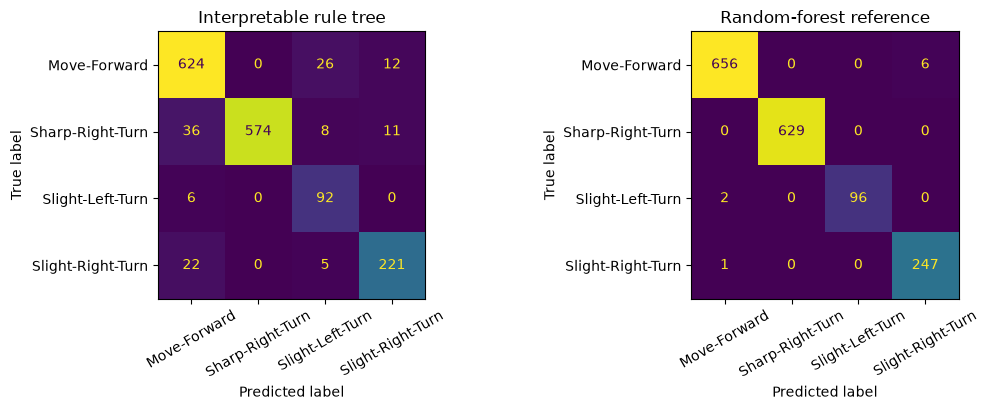
\includegraphics[width=.88\linewidth,height=5cm,keepaspectratio]{labs/visuals/05-notebook-reference.png}
\end{labvisual}
\begin{refoutput}
\begin{lstlisting}[style=utpterminal]
                     model  accuracy  macro_precision  macro_recall  macro_f1
0  Interpretable rule tree     0.923            0.879         0.921     0.895
1  Random-forest reference     0.995            0.993         0.992     0.992
Hardest action for the rule controller (lowest recall): Slight-Right-Turn
\end{lstlisting}
\end{refoutput}

\textbf{What it means.} The four-sensor tree reaches about 92\,\% accuracy and 0.90 macro F1; the all-sensor forest reaches over 99\,\% on both. The rule controller's weakest action is Slight-Right-Turn, and 22 of its 27 misses are called Move-Forward: the line between carrying on and nudging right sits on thresholds that a few centimetres can cross. That is the accuracy cost of a controller a person can read.
\end{labanswer}

\begin{labquestion}{6}{Test robustness to sensor noise}
Add zero-mean Gaussian noise to the test readings at 2, 5 and 10\,\% of the training-set standard deviation of each selected sensor, and plot the rule controller's macro F1 against the noise level.
\end{labquestion}
\begin{labanswer}
\lstinputlisting[style=utppython,firstline=99,lastline=116]{all_experiments/lab05_robotics_sensor_control_worked.py}
\begin{refoutput}
\begin{lstlisting}[style=utpterminal]
noise   0%: 0.895     2%: 0.858     5%: 0.787     10%: 0.706
Saved: ['confusion_matrices.png', 'feature_scores.csv', 'metrics.csv', 'noise_robustness.csv', 'noise_robustness.png', 'rule_controller.txt', 'rule_per_class.csv', 'split.csv']
\end{lstlisting}
\end{refoutput}

\textbf{What it means.} Macro F1 falls steadily as noise pushes readings across thresholds. Even 5\,\% of one standard deviation costs about eleven points, because a hard threshold has no margin: a reading on the wrong side by one millimetre gets the other action.
\end{labanswer}

\begin{yourturn}
Add new cells at the end of the notebook for these three tasks.
\begin{enumerate}
  \item \textbf{Trace one test row.} Row 265 reads US14 $=1.173$, US17 $=0.718$, US18 $=0.686$ and US13 $=5.0$. Follow it through \texttt{rule\_controller.txt} by hand, then confirm with \texttt{rule\_model.predict(X.loc[[265], selected])}. Now change US14 to $0.85$ in a copy of the row and predict the new action.
  \item \textbf{How many sensors?} Rerun the validation comparison at depth 5 with the top 1, 2, 4, 8 and 24 sensors from \texttt{feature\_table}. Use validation rows only. Where do extra sensors stop paying for themselves?
  \item \textbf{Respond to a 5\,\% noise budget.} Try two responses and compare their macro F1 on test readings with 5\,\% noise: retrain the four-sensor tree on noisy training readings, and fit a tree of depth 8 on the top eight sensors. State the cost of each.
\end{enumerate}
\end{yourturn}

\begin{expectedfindings}
\begin{enumerate}
  \item US14 $>0.90$; US18 $\le1.00$ and $>0.50$; US13 $>0.90$; US17 $>0.49$: \textbf{Move-Forward}, which is also the true action. With US14 at $0.85$ the very first rule fires: \textbf{Sharp-Right-Turn}.
  \item Validation macro F1 is 0.544, 0.803, 0.887, 0.943 and 0.967. The jump from one to four sensors is large, and after that each gain costs more sensors for less.
  \item Retraining the four-sensor tree on noisy readings barely helps (about 0.79 on noisy readings) and costs clean performance (about 0.83 on clean readings). Eight sensors at depth 8 give about 0.82 on noisy readings and 0.94 on clean readings, at the price of 23 leaves instead of 14 and twice the sensors to maintain. Your numbers will vary a little with the random seed for the noise.
\end{enumerate}
\end{expectedfindings}

\begin{troubleshoot}
\begin{description}
  \item[Sensor names look wrong] The file has no header, so \texttt{header=None} and \texttt{names=...} must both be present, as in Question~1.
  \item[A feature-name warning at \texttt{predict}] You passed a NumPy array to a model fitted on a DataFrame. Wrap it in \texttt{pd.DataFrame(values, columns=selected)}.
  \item[Test scores much higher than the reference] You probably selected sensors or depth using test rows. Check that every \texttt{fit} before Question~5 uses training rows only.
\end{description}
\end{troubleshoot}

\begin{verification}
\begin{itemize}
  \item The 5,456 readings are split 70/30 with stratification, and the split is saved.
  \item The four sensors are selected by mutual information on the training rows only.
  \item The tree depth is chosen by validation macro F1, and the final tree is exported as readable if--then rules.
  \item On the test rows the rule controller reaches about 92\,\% accuracy and 0.90 macro F1, and its hardest action is identified.
  \item Macro F1 is reported at every noise level, and you can explain why it falls.
\end{itemize}
\end{verification}

\begin{labdeliverable}
\begin{itemize}
  \item Restart the kernel and run all cells without errors.
  \item Submit the executed notebook, including your \emph{Your turn} cells, and the generated \texttt{results/lab05/} folder.
  \item Add a short conclusion: identify the hardest action, and recommend one response to a 5\,\% sensor-noise budget, including its trade-off.
\end{itemize}
\end{labdeliverable}


\labsection{5}{Robotics: Sensor-to-Action Control}{sec:lab05-robotics}

\begin{labproject}{Build and evaluate an interpretable wall-following controller}
\textbf{Read first.} Chapter~\ref{ch:robotics}.\\
\textbf{Goal.} Derive a four-sensor threshold policy, compare it with an all-sensor reference model, and test its sensitivity to sensor noise.\\
\textbf{Scenario.} A SCITOS G5 robot must convert 24 ultrasonic readings into one of four movement commands while following a wall.\\
\textbf{Data.} \texttt{all\_datasets/lab05-sensor\_readings\_24.csv} (5,456 readings, no header: 24 distances in metres, then the action).\\
\textbf{Notebook.} \texttt{all\_experiments/lab05\_robotics\_sensor\_control\_worked.ipynb}.\\
\textbf{Hand in.} The executed notebook, the \texttt{results/lab05/} folder and a short conclusion, as listed in the checklist at the end of this sheet.
\end{labproject}

\begin{labmode}
\begin{enumerate}
  \item Activate your course environment and confirm that the data file is in \texttt{all\_datasets/}.
  \item Start Jupyter from \texttt{all\_experiments/}, open the notebook, and choose \textbf{Restart Kernel and Run All Cells}. Everything runs in a few seconds.
\end{enumerate}
\begin{lstlisting}[style=utpterminal]
cd all_experiments
jupyter lab
\end{lstlisting}
Prefer a plain script? From the course folder, \texttt{python all\_experiments/lab05\_robotics\_sensor\_control\_worked.py} runs the same code and writes the same evidence.
\end{labmode}

\courselabflow{Split readings}{Select sensors}{Fit controller}{Test noise}


\labroutine

\begin{yourturn}
\textbf{Warm-up on paper.} Using the first levels of the learned tree in \figref{fig:tree-rules}, decide what the controller does for these readings: (a) US14 $=0.81$; (b) US14 $=1.94$, US18 $=5.00$, US17 $=1.44$. Say in plain words what is happening around the robot in each case.

\emph{Answer.} (a) Sharp-Right-Turn: the wall is close on the rear left, so steer away. (b) US14 and US18 are both large and US17 is above 0.90, so the tree goes down the branch that mostly says Slight-Left-Turn: the wall has fallen away, so edge back towards it.
\end{yourturn}

\textbf{Setup.} Run the imports and path setup first, and keep this kernel state for the later questions. In the script version the first seven lines also set the working directory.
\lstinputlisting[style=utppython,firstline=1,lastline=7]{all_experiments/lab05_robotics_sensor_control_worked.py}
\lstinputlisting[style=utppython,firstline=8,lastline=23]{all_experiments/lab05_robotics_sensor_control_worked.py}

\begin{labquestion}{1}{Inspect the data and fix the split}
The CSV has no header: 24 ultrasonic distances (metres) followed by the action label. Name the columns, report the class balance and sensor summary statistics, and create a fixed stratified 70/30 train/test split with seed 42. Save the split.
\end{labquestion}
\begin{labanswer}
\courselabtrace{Protect the evaluation boundary}{Training}{Select four sensors and learn thresholds}{Test}{Apply the frozen policy to unseen readings}{Noise}{Perturb test sensors; keep labels unchanged}

\lstinputlisting[style=utppython,firstline=25,lastline=38]{all_experiments/lab05_robotics_sensor_control_worked.py}
\begin{refoutput}
\begin{lstlisting}[style=utpterminal]
Shape: (5456, 25)
Move-Forward 2205 (0.404)   Sharp-Right-Turn 2097 (0.384)
Slight-Right-Turn 826 (0.151)   Slight-Left-Turn 328 (0.060)
{'train': 3819, 'test': 1637}
\end{lstlisting}
\end{refoutput}

\textbf{What it means.} The classes are imbalanced, so accuracy alone would flatter a model that ignores the small classes, and macro F1 is reported throughout. Sensor readings are distances in metres between 0.4~m and 5~m. Stratification keeps the class shares equal in the 3,819 training and 1,637 test rows. The notebook numbers the sensors from US00, the front sensor, clockwise to US23.
\end{labanswer}

\begin{labquestion}{2}{Select four sensors using training data only}
Rank the 24 sensors by mutual information with the action, computed on the training rows only, and keep the top four for the interpretable controller. Save the full ranking.
\end{labquestion}
\begin{labanswer}
Read \texttt{selected} rather than hard-coding the names from a saved run:
\courselabtrace{Trace training-only sensor selection}{1. Input / state}{X has US00 through US23; train\_idx and test\_idx preserve the stratified split.}{2. Operation}{Compute mi on X.loc[train\_idx] and training actions; sort feature\_table and take its first four sensor names.}{3. Check}{selected is reused, in the same order, for tree fitting and held-out predictions.}


\lstinputlisting[style=utppython,firstline=40,lastline=45]{all_experiments/lab05_robotics_sensor_control_worked.py}
\begin{refoutput}
\begin{lstlisting}[style=utpterminal]
Selected sensors: ['US14', 'US17', 'US18', 'US13']
\end{lstlisting}
\end{refoutput}

\textbf{What it means.} The four most informative sensors come from the same rear-left arc of the ring, which is what a wall follower needs: the distance to the wall it is tracking, seen from slightly different angles. Selecting on training rows only keeps the test set untouched.
\end{labanswer}

\textbf{Connect it to the chapter.} The next questions fill in the ``think'' box of this loop. Remember that the dashed arrow is not tested here.
% Reused from chapters/05-robotics-scenarios.tex
\begin{labvisual}{Recall the chapter model}
\begin{labgraphic}
\begin{tikzpicture}[font=\small]
\node[utpbox,minimum width=2.9cm,minimum height=1.1cm] (sense) at (0,0) {\textbf{Sense}\\24 ultrasonic distances};
\node[utpbox,minimum width=2.9cm,minimum height=1.1cm,fill=UTPPaleOrange,draw=UTPOrange,line width=1pt] (think) at (4.6,0) {\textbf{Think}\\readings $\to$ action};
\node[utpbox,minimum width=2.9cm,minimum height=1.1cm] (act) at (9.2,0) {\textbf{Act}\\one of four motions};
\node[utpbox,minimum width=3.4cm,minimum height=0.9cm,fill=UTPPaleGray,draw=UTPMuted] (world) at (4.6,-2.2) {the room: walls, corners, doorways};
\draw[utparrow] (sense)--(think);
\draw[utparrow] (think)--(act);
\draw[utparrow] (act.south) |- (world.east);
\draw[utparrow,dashed] (world.west) -| (sense.south);
\node[utplabel,anchor=south,color=UTPOrange] at (4.6,0.75) {Lab~5: this box is learned from 5,456 logged pairs};
\node[utplabel,anchor=north,color=UTPMuted] at (4.6,-2.72) {dashed arrow: feedback --- the next reading depends on this action};
\end{tikzpicture}
\end{labgraphic}\end{labvisual}


\begin{labquestion}{3}{Fit an interpretable rule controller}
A shallow decision tree is a fixed set of threshold rules. Carve an internal validation set out of the training rows, choose the tree depth by validation macro F1, refit on all training rows, and export the final tree as explicit if--then rules.
\end{labquestion}
\begin{labanswer}
\lstinputlisting[style=utppython,firstline=47,lastline=65]{all_experiments/lab05_robotics_sensor_control_worked.py}
\begin{refoutput}
\begin{lstlisting}[style=utpterminal]
depth 2: 0.463   depth 3: 0.826   depth 4: 0.872   depth 5: 0.887   depth 6: 0.883
Selected depth: 5 | leaves: 14
|--- US14 <= 0.90
|   |--- class: Sharp-Right-Turn
|--- US14 >  0.90
|   |--- US18 <= 1.00
...
\end{lstlisting}
\end{refoutput}

\textbf{What it means.} Validation macro F1 climbs steeply from depth 2 to 4 and flattens at depth 5, which is selected. The exported tree reads as a policy. Its very first split, \emph{if the wall-side sensor US14 reads less than 0.9~m, turn sharply right}, is the wall-following reflex, and the deeper splits refine the slight turns. Every decision is a threshold a robotics engineer can inspect.
\end{labanswer}

\begin{labquestion}{4}{Fit a reference model}
Train a random forest on all 24 sensors using the same training partition. It is not interpretable; its purpose is to show what accuracy the four-sensor rule controller gives up.
\end{labquestion}
\begin{labanswer}
\lstinputlisting[style=utppython,firstline=67,lastline=70]{all_experiments/lab05_robotics_sensor_control_worked.py}
\begin{refoutput}
\begin{lstlisting}[style=utpterminal]
Random forest trained on 24 sensors with 200 trees
\end{lstlisting}
\end{refoutput}

\textbf{What it means.} The forest uses every sensor and 200 trees, so it can exploit interactions the shallow tree cannot. It is the reference ceiling, not a candidate controller.
\end{labanswer}

\begin{labquestion}{5}{Evaluate on the held-out data}
Report accuracy, macro precision, macro recall and macro F1 for both models on the test rows, draw both confusion matrices, list per-class recall for the rule controller, and identify its hardest action.
\end{labquestion}
\begin{labanswer}
\lstinputlisting[style=utppython,firstline=72,lastline=97]{all_experiments/lab05_robotics_sensor_control_worked.py}
\begin{labvisual}{Reference plot from the supplied notebook}
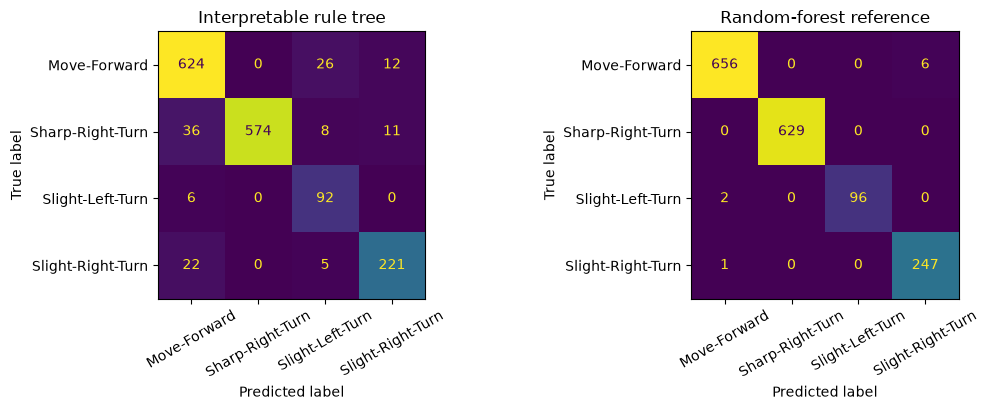
\includegraphics[width=.88\linewidth,height=5cm,keepaspectratio]{labs/visuals/05-notebook-reference.png}
\end{labvisual}
\begin{refoutput}
\begin{lstlisting}[style=utpterminal]
                     model  accuracy  macro_precision  macro_recall  macro_f1
0  Interpretable rule tree     0.923            0.879         0.921     0.895
1  Random-forest reference     0.995            0.993         0.992     0.992
Hardest action for the rule controller (lowest recall): Slight-Right-Turn
\end{lstlisting}
\end{refoutput}

\textbf{What it means.} The four-sensor tree reaches about 92\,\% accuracy and 0.90 macro F1; the all-sensor forest reaches over 99\,\% on both. The rule controller's weakest action is Slight-Right-Turn, and 22 of its 27 misses are called Move-Forward: the line between carrying on and nudging right sits on thresholds that a few centimetres can cross. That is the accuracy cost of a controller a person can read.
\end{labanswer}

\begin{labquestion}{6}{Test robustness to sensor noise}
Add zero-mean Gaussian noise to the test readings at 2, 5 and 10\,\% of the training-set standard deviation of each selected sensor, and plot the rule controller's macro F1 against the noise level.
\end{labquestion}
\begin{labanswer}
\lstinputlisting[style=utppython,firstline=99,lastline=116]{all_experiments/lab05_robotics_sensor_control_worked.py}
\begin{refoutput}
\begin{lstlisting}[style=utpterminal]
noise   0%: 0.895     2%: 0.858     5%: 0.787     10%: 0.706
Saved: ['confusion_matrices.png', 'feature_scores.csv', 'metrics.csv', 'noise_robustness.csv', 'noise_robustness.png', 'rule_controller.txt', 'rule_per_class.csv', 'split.csv']
\end{lstlisting}
\end{refoutput}

\textbf{What it means.} Macro F1 falls steadily as noise pushes readings across thresholds. Even 5\,\% of one standard deviation costs about eleven points, because a hard threshold has no margin: a reading on the wrong side by one millimetre gets the other action.
\end{labanswer}

\begin{yourturn}
Add new cells at the end of the notebook for these three tasks.
\begin{enumerate}
  \item \textbf{Trace one test row.} Row 265 reads US14 $=1.173$, US17 $=0.718$, US18 $=0.686$ and US13 $=5.0$. Follow it through \texttt{rule\_controller.txt} by hand, then confirm with \texttt{rule\_model.predict(X.loc[[265], selected])}. Now change US14 to $0.85$ in a copy of the row and predict the new action.
  \item \textbf{How many sensors?} Rerun the validation comparison at depth 5 with the top 1, 2, 4, 8 and 24 sensors from \texttt{feature\_table}. Use validation rows only. Where do extra sensors stop paying for themselves?
  \item \textbf{Respond to a 5\,\% noise budget.} Try two responses and compare their macro F1 on test readings with 5\,\% noise: retrain the four-sensor tree on noisy training readings, and fit a tree of depth 8 on the top eight sensors. State the cost of each.
\end{enumerate}
\end{yourturn}

\begin{expectedfindings}
\begin{enumerate}
  \item US14 $>0.90$; US18 $\le1.00$ and $>0.50$; US13 $>0.90$; US17 $>0.49$: \textbf{Move-Forward}, which is also the true action. With US14 at $0.85$ the very first rule fires: \textbf{Sharp-Right-Turn}.
  \item Validation macro F1 is 0.544, 0.803, 0.887, 0.943 and 0.967. The jump from one to four sensors is large, and after that each gain costs more sensors for less.
  \item Retraining the four-sensor tree on noisy readings barely helps (about 0.79 on noisy readings) and costs clean performance (about 0.83 on clean readings). Eight sensors at depth 8 give about 0.82 on noisy readings and 0.94 on clean readings, at the price of 23 leaves instead of 14 and twice the sensors to maintain. Your numbers will vary a little with the random seed for the noise.
\end{enumerate}
\end{expectedfindings}

\begin{troubleshoot}
\begin{description}
  \item[Sensor names look wrong] The file has no header, so \texttt{header=None} and \texttt{names=...} must both be present, as in Question~1.
  \item[A feature-name warning at \texttt{predict}] You passed a NumPy array to a model fitted on a DataFrame. Wrap it in \texttt{pd.DataFrame(values, columns=selected)}.
  \item[Test scores much higher than the reference] You probably selected sensors or depth using test rows. Check that every \texttt{fit} before Question~5 uses training rows only.
\end{description}
\end{troubleshoot}

\begin{verification}
\begin{itemize}
  \item The 5,456 readings are split 70/30 with stratification, and the split is saved.
  \item The four sensors are selected by mutual information on the training rows only.
  \item The tree depth is chosen by validation macro F1, and the final tree is exported as readable if--then rules.
  \item On the test rows the rule controller reaches about 92\,\% accuracy and 0.90 macro F1, and its hardest action is identified.
  \item Macro F1 is reported at every noise level, and you can explain why it falls.
\end{itemize}
\end{verification}

\begin{labdeliverable}
\begin{itemize}
  \item Restart the kernel and run all cells without errors.
  \item Submit the executed notebook, including your \emph{Your turn} cells, and the generated \texttt{results/lab05/} folder.
  \item Add a short conclusion: identify the hardest action, and recommend one response to a 5\,\% sensor-noise budget, including its trade-off.
\end{itemize}
\end{labdeliverable}


\part{Language Intelligence}
\chapter{NLP Foundations: Getting Text and Measuring It}
\label{ch:nlp-foundations}

\chapterguide%
  {Manipulate Python strings, and know what a controlled experiment is.}
  {describe an NLP pipeline from raw input to task output; explain why text normalisation comes before any comparison; compute Levenshtein distance by hand and turn it into character error rate; design a fair before/after comparison of a preprocessing step; and separate segmentation failures from recognition failures in an OCR error analysis.}

Natural language processing (NLP) starts before there is any language to process, because text has to come from somewhere: keystrokes, speech or images. Lab~6 applies optical character recognition to 89 photographs of handwritten medicine names and asks: \emph{how good is the resulting text, and how should we measure it?}

\section{Every NLP task is a pipeline}

NLP systems acquire text, normalise it, build a representation, apply a task model and evaluate the output (\figref{fig:nlp-pipeline}).

\begin{analogy}
Think of an assembly line. A part that falls off at the first station is simply missing at every station after it, however good those later stations are. Early errors in NLP work the same way: no downstream model can use a word that OCR never saw.
\end{analogy}

\begin{utpfig}[The NLP pipeline]{Lab~6 covers acquisition, normalisation and OCR measurement. Lab~7 starts with clean text and builds a representation and classifier.}{fig:nlp-pipeline}
\begin{tikzpicture}[scale=0.99,transform shape,
  b/.style={draw=UTPBlue,fill=UTPPaleBlue,rounded corners=2mm,minimum width=2.20cm,minimum height=1.0cm,align=center,font=\small\color{UTPNavy}},
  arr/.style={-{Stealth[length=2mm]},thick,draw=UTPTeal}
]
\node[b] (acq) {Acquire\\\scriptsize photo, audio, keyboard};
\node[b,right=0.26cm of acq] (norm) {Normalise\\\scriptsize case, punctuation, tokens};
\node[b,right=0.26cm of norm] (rep) {Represent\\\scriptsize counts, n-grams, vectors};
\node[b,right=0.26cm of rep] (model) {Model\\\scriptsize classify, translate, search};
\node[b,right=0.26cm of model] (eval) {Evaluate\\\scriptsize against references};
\draw[arr] (acq)--(norm); \draw[arr] (norm)--(rep); \draw[arr] (rep)--(model); \draw[arr] (model)--(eval);
\draw[utpbrace,decoration={mirror},draw=UTPOrange] (-1.3,-0.75) -- (3.9,-0.75);
\node[font=\scriptsize\color{UTPOrange},anchor=north] at (1.3,-0.95) {Lab~6: OCR, normalisation, measurement};
\draw[utpbrace,decoration={mirror},draw=UTPGreen] (4.1,-0.75) -- (12.0,-0.75);
\node[font=\scriptsize\color{UTPGreen},anchor=north] at (8.1,-0.95) {Lab~7: bag of words, Naive Bayes, evaluation};
\end{tikzpicture}
\end{utpfig}

\section{Optical character recognition as text acquisition}

\term{OCR} converts images to strings. Tesseract, the engine used in the lab, works in two stages. \term{Segmentation} locates the text on the page, and a neural \term{recognition} stage reads what it found. Keeping the stages apart in your head matters, because they fail differently: one misses text altogether, the other misreads it.

Lab~6 fixes \texttt{--oem 1} (neural recognition) and \texttt{--psm 7} (treat the image as a single line of text) for every cropped name. Holding these settings constant isolates the effect of preprocessing.

\begin{intuition}
Tesseract was built mainly for print, not for cursive on lined paper. Asking it to read a doctor's handwriting is like asking someone who learned a language from textbooks to follow a fast regional accent. Downstream processing cannot reliably recover what the recogniser missed.
\end{intuition}

\section{Normalisation before comparison}

``Tab Azimax'' and ``tab azimax'', or ``40 mg'' and ``40mg'', differ as strings. If we compared raw strings, a capital letter would count as an error just like a wrong drug name. Lab~6 therefore reduces predictions and references to lowercase letters and digits before comparing them:

\lstinputlisting[style=utppython,firstline=69,lastline=70]{all_experiments/lab06_handwriting_ocr_worked.py}

This rule excludes case, spacing and punctuation from the error count. A task that must distinguish ``40 mg'' from ``4 0mg'' needs a different rule, and its scores are not directly comparable with these. The choice is visible in the numbers: on the raw baseline the character error rate is 0.88 with this normaliser, 0.88 if spaces are kept, and 0.93 with no normalisation at all.

\begin{keyidea}
Normalise both sides identically, decide in advance which differences count as errors, and write the rule down. A metric is only meaningful relative to the normalisation it was computed under.
\end{keyidea}

\section{Measuring text quality: edit distance}

\term{Exact match} requires identical normalised strings, and none of the 89 baseline predictions qualifies. That single number hides a lot. Reading \texttt{dicloran} as \texttt{diclorew} is nearly right, while reading it as nothing at all is useless, yet exact match scores both as zero. We need a graded measure.

\term{Levenshtein distance} gives one: the minimum number of single-character insertions, deletions and substitutions needed to turn one string into the other. Imagine a proofreader correcting the OCR output with a red pen and charging one unit per mark. The distance is the smallest possible bill (\figref{fig:levenshtein}).

\begin{utpfig}[Levenshtein distance by dynamic programming]{The table for turning the reference \texttt{nims} into the OCR output \texttt{nidu}, as Lab~6's baseline actually read it. Cell $(i,j)$ holds the cost of matching the first $i$ characters of the reference with the first $j$ of the prediction: one more than the cell above (delete), one more than the cell to the left (insert), or the diagonal plus one if the characters differ (substitute). The answer, 2, is in the bottom-right corner: substitute \texttt{m}$\to$\texttt{d} and \texttt{s}$\to$\texttt{u}.}{fig:levenshtein}
\begin{tikzpicture}[font=\small]
\def\W{0.78}
\foreach \c [count=\ci from 1] in {n,i,d,u}{\node[font=\bfseries\color{UTPOrange}] at (\W*\ci,\W*0.85) {\c};}
\foreach \r [count=\ri from 1] in {n,i,m,s}{\node[font=\bfseries\color{UTPBlue}] at (-\W*0.85,-\W*\ri) {\r};}
\foreach \row [count=\ri from 0] in {{0,1,2,3,4},{1,0,1,2,3},{2,1,0,1,2},{3,2,1,1,2},{4,3,2,2,2}}{
  \foreach \v [count=\ci from 0] in \row{
    \ifnum\ri=\ci
      \node[utphot,minimum width=\W cm,minimum height=\W cm,font=\scriptsize\bfseries] at (\W*\ci,-\W*\ri) {\v};
    \else
      \node[utpcell,minimum width=\W cm,minimum height=\W cm,font=\scriptsize] at (\W*\ci,-\W*\ri) {\v};
    \fi
  }
}
\node[utplabel,anchor=north,color=UTPBlue] at (-\W*0.85,-\W*4.6) {reference};
\node[utplabel,anchor=south,color=UTPOrange] at (\W*2.5,\W*1.3) {prediction};
\node[utplabel,anchor=west,align=left,text width=6.2cm] at (\W*5.4,-\W*1.2)
  {$D[i,j]=\min\big(D[i-1,j]+1,\ D[i,j-1]+1,\ D[i-1,j-1]+[r_i\neq p_j]\big)$\\[4pt]
   The highlighted diagonal is the cheapest path: match \texttt{n}, match \texttt{i}, substitute, substitute.\\[4pt]
   Distance $=2$; normalised by the longer length, $2/4=0.5$.};
\end{tikzpicture}
\end{utpfig}

The lab's implementation computes that table one row at a time, keeping only the previous row:

\lstinputlisting[style=utppython,firstline=104,lastline=112]{all_experiments/lab06_handwriting_ocr_worked.py}

The lab reports three distance-based metrics and a separate blank count:

\begin{utptable}
\begin{tabularx}{\linewidth}{@{}>{\bfseries\leavevmode\color{UTPNavy}}m{0.30\linewidth}m{0.30\linewidth}X@{}}
\toprule
\rowcolor{UTPPaleBlue!92}
\utpth{Metric} & \utpth{Definition} & \utpth{Answers} \\
\midrule
Exact-match accuracy & Fraction of images with distance $0$ & How often is the name usable as-is? \\
Mean normalised edit distance & Mean over images of distance $/$ longer length; in $[0,1]$ & How wrong is a typical image? \\
Character error rate (CER) & Total edits $/$ total reference characters; can exceed $1$ & How many corrections per 100 reference characters? \\
Blank predictions & Images whose normalised prediction is empty & How often did segmentation find nothing? \\
\bottomrule
\end{tabularx}
\end{utptable}

\begin{workedexample}
Take two images. Reference \texttt{nims} is read as \texttt{nidu}: 2 edits on 4 characters. Reference \texttt{tabnims100mg} is read as nothing: 12 edits on 12 characters.

\[
\text{mean normalised distance}=\frac{2/4+12/12}{2}=0.75,
\qquad
\text{CER}=\frac{2+12}{4+12}=0.875.
\]

The mean treats both images equally. CER pools the characters, so the long name counts for more.
\end{workedexample}

\begin{pitfall}
CER is a ratio of totals, so long references dominate it. The normalised distance is a mean of per-image ratios, so every image counts equally. The two can move in opposite directions on the same data. Report both, and say which one a decision rests on.
\end{pitfall}

\section{A controlled preprocessing experiment}

The baseline has CER near $0.9$ and 44 blank predictions. Lab~6 tests one fixed preprocessing pipeline: grayscale, a 20-pixel white border, a width cap and $1.5\times$ enlargement. These steps target colour noise, text touching the image edge and character size, and they leave the OCR settings alone.

Use the same 89 images, the same normalisation and the same OCR configuration, so that only the image preprocessing changes. A fair experiment changes one thing.

\begin{utptable}
\begin{tabularx}{\linewidth}{@{}>{\bfseries\leavevmode\color{UTPNavy}}m{0.30\linewidth}>{\centering\arraybackslash}X>{\centering\arraybackslash}X>{\centering\arraybackslash}X>{\centering\arraybackslash}X@{}}
\toprule
\rowcolor{UTPPaleBlue!92}
\utpth{Pipeline} & \utpth{Exact match} & \utpth{Norm.\ edit distance} & \utpth{CER} & \utpth{Blank} \\
\midrule
Raw images & 0.000 & 0.860 & 0.881 & 44 \\
Grayscale, border, resize & 0.011 & 0.767 & 0.788 & 15 \\
\bottomrule
\end{tabularx}
\end{utptable}

Blanks fall from 44 to 15 and CER falls by about $0.09$, but only one image, \texttt{ostium}, becomes an exact match. Look past the totals and the picture is more mixed. Measured by edits, 43 images improved, 18 got worse and 28 did not change. Thirty-four images that were blank now yield text, while 5 that yielded text are now blank: \texttt{tab mesulid}, for instance, was read as \texttt{wos Mesulia} on the raw image and not at all after preprocessing. On balance preprocessing helps segmentation find text, and it leaves substantial recognition errors behind.

\section{Error analysis: which stage failed?}

Lab~6 sorts predictions by normalised edit distance and tags the worst cases. It keeps all 89 samples, records any OCR-engine exception instead of dropping the image, and assigns each difficult case one of three reproducible labels. If Tesseract is not installed, the notebook identifies the run as \emph{cached} and loads the validated predictions supplied with the course package; it never presents cached text as a live run.

\begin{description}
  \item[Engine error.] Tesseract rejects an individual image. The sample stays in the benchmark as a failed recognition, with the error recorded in \texttt{predictions.csv}.
  \item[No text detected.] An empty normalised prediction suggests missed text, for example from faint strokes, low contrast or slanted writing. Preprocessing may help. Seven of the eight worst preprocessed cases are of this kind.
  \item[Character confusion.] Text is returned but misread: \texttt{provas} as \texttt{Pras}, or \texttt{starcox 90} as \texttt{Stak Oe 90}. Persistent handwriting errors point to the need for a recogniser trained on handwriting.
\end{description}

Save the six hardest images with their references and predictions, so readers can check the tags for themselves.

\begin{keyidea}
Attribute each failure to the stage that produced it. The fix for ``no text found'' is different from the fix for ``wrong text found'', and an aggregate score cannot tell them apart.
\end{keyidea}

\section{Fitness for purpose}

The benchmark shows a poor fit between printed-text OCR and cursive handwriting, not evidence for clinical use. Misread medicine names or doses can cause real harm. Clinical transcription would require a handwriting-specific recogniser, representative data, held-out validation, privacy controls and human review of uncertain readings.

\begin{chapterrecap}
\begin{itemize}
  \item NLP is a pipeline, and errors made early cannot be repaired later.
  \item Normalise references and predictions by one written rule before comparing them. A metric means nothing without it.
  \item Levenshtein distance counts the fewest single-character edits, and normalised distance and CER aggregate it in two different ways.
  \item Change one thing at a time. Preprocessing cut blanks from 44 to 15 but barely moved exact matches.
  \item Attribute each failure to segmentation or recognition, because they need different fixes.
\end{itemize}
\end{chapterrecap}

\begin{quickcheck}
\begin{enumerate}
  \item How do an engine error, a blank prediction, and \texttt{nims} being read as \texttt{nidu} differ?
  \item Compute the Levenshtein distance between \texttt{breeky} and \texttt{beeky}, and the normalised distance.
  \item Why must the OCR configuration stay fixed when the preprocessing pipeline is tested?
  \item After preprocessing, CER fell by $0.09$ but exact-match accuracy rose by only one image. What does that pattern say about which stage improved?
  \item The lab's normaliser deletes spaces. Name a task for which that would be the wrong choice.
\end{enumerate}
\end{quickcheck}

\begin{checkanswers}
\begin{enumerate}
  \item An engine error is a recorded runtime failure of Tesseract on that image; a blank prediction means the segmenter found no text line; \texttt{nidu} means a line was found but the recogniser misread its characters. Only the last is a recognition failure.
  \item Delete one \texttt{r}: distance $1$. Normalised by the longer length, $1/6\approx0.17$.
  \item Otherwise an improvement could come from the engine settings rather than from the images. A controlled experiment changes one factor at a time.
  \item The segmentation stage improved, since many more images now yield some text, while the recognition stage still misreads cursive, so few of those texts are exactly right.
  \item Any task in which spacing carries meaning: distinguishing ``40 mg'' from ``4 0mg'', counting words, or matching multi-word names.
\end{enumerate}
\end{checkanswers}

\labsection{6}{NLP Foundations: Handwriting OCR Evaluation}{sec:lab06-nlp-a}

\begin{labproject}{Evaluate OCR on real handwritten medicine names}
\textbf{Read first.} Chapter~\ref{ch:nlp-foundations}.\\
\textbf{Goal.} Benchmark OCR on 89 labelled images, test one controlled preprocessing pipeline, and classify the failures.\\
\textbf{Scenario.} A clinic wants to digitise handwritten medicine names before storage or search.\\
\textbf{Data.} \texttt{all\_datasets/lab06-ocr-handwritten-prescription.zip}: one label CSV and 89 images. The notebook extracts it next to the archive.\\
\textbf{Notebook.} \texttt{all\_experiments/lab06\_handwriting\_ocr\_worked.ipynb}.\\
\textbf{Hand in.} The executed notebook, the \texttt{results/lab06/} folder and a short conclusion, as listed in the checklist at the end of this sheet.
\end{labproject}

\begin{labmode}
\begin{enumerate}
  \item Activate your course environment and confirm that the zip is in \texttt{all\_datasets/}. Do not extract it yourself; the notebook does that.
  \item \textbf{Install the Tesseract OCR engine.} This is the one lab that needs software beyond Python. The \texttt{pytesseract} package in \texttt{requirements.txt} is only a wrapper around it. Use the line for your system, then reopen the terminal and check the version.
  \item Start Jupyter from \texttt{all\_experiments/}, open the notebook, and choose \textbf{Restart Kernel and Run All Cells}.
\end{enumerate}
\begin{lstlisting}[style=utpterminal]
# Windows (PowerShell)
winget install --id UB-Mannheim.TesseractOCR -e

# macOS
brew install tesseract

# Debian or Ubuntu
sudo apt install tesseract-ocr

# Every system: check it, then start the lab
tesseract --version
cd all_experiments
jupyter lab
\end{lstlisting}
On Windows the notebook also looks in \texttt{C:\textbackslash Program Files\textbackslash Tesseract-OCR}, so it finds a default install even if the terminal does not.
\end{labmode}

\begin{pitfall}
\textbf{Live or cached?} With Tesseract and its Python wrapper installed, this lab performs live recognition, and the first printed line says \texttt{OCR mode: live}. Otherwise it analyses the supplied predictions in \texttt{results/lab06/predictions.csv} and says \texttt{OCR mode: cached}. A cached run can reproduce the saved comparison and every metric, but it cannot test a new preprocessing choice. Never describe a cached run as new OCR inference. Keep \texttt{predictions.csv} in place, because cached mode reads it.
\end{pitfall}

\courselabflow{Extract images}{Run OCR}{Normalise text}{Compare errors}


\labroutine

\begin{yourturn}
\textbf{Warm-up on paper.} The raw baseline reads \texttt{dicloran} as \texttt{diclerew}. Work out the Levenshtein distance by hand, using the table method of \figref{fig:levenshtein}, and then the normalised distance.

\emph{Answer.} Substitute \texttt{o}$\to$\texttt{e}, \texttt{a}$\to$\texttt{e} and \texttt{n}$\to$\texttt{w}: distance 3. Both strings have 8 characters, so the normalised distance is $3/8=0.375$.
\end{yourturn}

\textbf{Setup.} Run the imports and path setup first, and keep this kernel state for the later questions. In the script version the first seven lines also set the working directory.
\lstinputlisting[style=utppython,firstline=1,lastline=7]{all_experiments/lab06_handwriting_ocr_worked.py}
\lstinputlisting[style=utppython,firstline=8,lastline=40]{all_experiments/lab06_handwriting_ocr_worked.py}
\begin{refoutput}
\begin{lstlisting}[style=utpterminal]
OCR mode: live | Tesseract 5.5.3.20260724 at C:\Program Files\Tesseract-OCR\tesseract.exe
\end{lstlisting}
\end{refoutput}

\begin{labquestion}{1}{Validate the archive}
Extract the archive next to itself, load the label file, check that all 89 labelled images exist exactly once, report the number of unique labels, and show a 3-by-3 sample grid.
\end{labquestion}
\begin{labanswer}
\courselabtrace{Compare the same images twice}{Baseline}{Original image to recognised text}{Treatment}{Preprocess image, then use the same OCR engine}{Check}{Pair both predictions with the same true label}

\lstinputlisting[style=utppython,firstline=42,lastline=64]{all_experiments/lab06_handwriting_ocr_worked.py}
\begin{labvisual}{Reference plot from the supplied notebook}
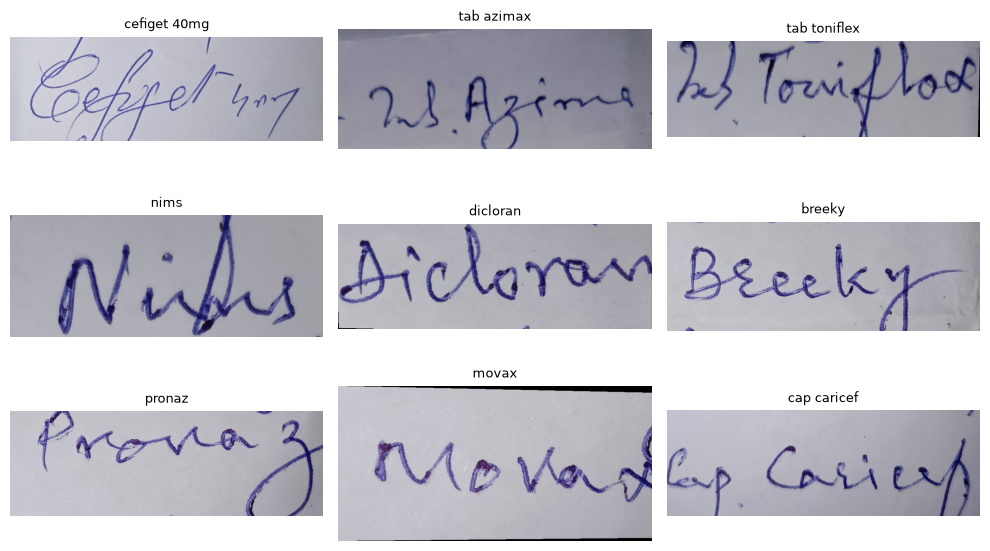
\includegraphics[width=.88\linewidth,height=5cm,keepaspectratio]{labs/visuals/06-notebook-reference.png}
\end{labvisual}
\begin{refoutput}
\begin{lstlisting}[style=utpterminal]
Labelled images: 89 | unique labels: 61
\end{lstlisting}
\end{refoutput}

\textbf{What it means.} One label file and 89 photographs, each present exactly once. The 89 labels hold 61 distinct medicine names, so some names appear several times in different handwriting. The grid shows what the engine faces: cursive, varied stroke width, uneven lighting and lined paper.
\end{labanswer}

\begin{labquestion}{2}{Run the baseline OCR}
Use one fixed Tesseract configuration for every raw image (LSTM engine, page-segmentation mode 7 = one text line) and normalise both prediction and label to lowercase letters and digits. Record a per-image engine failure instead of dropping the sample or stopping the benchmark.
\end{labquestion}
\begin{labanswer}
\lstinputlisting[style=utppython,firstline=66,lastline=102]{all_experiments/lab06_handwriting_ocr_worked.py}
\begin{refoutput}
\begin{lstlisting}[style=utpterminal]
          truth      prediction prediction_norm
0  cefiget 40mg
1    tab azimax              Ao              ao
2  tab toniflex  p53 Towid host    p53towidhost
3          nims            Nidu            nidu
4      dicloran        diclerew        diclerew
OCR engine errors: 0
\end{lstlisting}
\end{refoutput}

\textbf{What it means.} The first rows distinguish a blank recognition from a misread name while retaining every labelled image. The configuration is fixed, so any later improvement must come from the image rather than from engine tuning.
\end{labanswer}

\textbf{Connect it to the chapter.} The next questions measure the second and third boxes of this pipeline, and an error made in the first cannot be repaired by them.
% Reused from chapters/06-nlp-foundations.tex
\begin{labvisual}{Recall the chapter model}
\begin{labgraphic}
\begin{tikzpicture}[scale=0.99,transform shape,
  b/.style={draw=UTPBlue,fill=UTPPaleBlue,rounded corners=2mm,minimum width=2.20cm,minimum height=1.0cm,align=center,font=\small\color{UTPNavy}},
  arr/.style={-{Stealth[length=2mm]},thick,draw=UTPTeal}
]
\node[b] (acq) {Acquire\\\scriptsize photo, audio, keyboard};
\node[b,right=0.26cm of acq] (norm) {Normalise\\\scriptsize case, punctuation, tokens};
\node[b,right=0.26cm of norm] (rep) {Represent\\\scriptsize counts, n-grams, vectors};
\node[b,right=0.26cm of rep] (model) {Model\\\scriptsize classify, translate, search};
\node[b,right=0.26cm of model] (eval) {Evaluate\\\scriptsize against references};
\draw[arr] (acq)--(norm); \draw[arr] (norm)--(rep); \draw[arr] (rep)--(model); \draw[arr] (model)--(eval);
\draw[utpbrace,decoration={mirror},draw=UTPOrange] (-1.3,-0.75) -- (3.9,-0.75);
\node[font=\scriptsize\color{UTPOrange},anchor=north] at (1.3,-0.95) {Lab~6: OCR, normalisation, measurement};
\draw[utpbrace,decoration={mirror},draw=UTPGreen] (4.1,-0.75) -- (12.0,-0.75);
\node[font=\scriptsize\color{UTPGreen},anchor=north] at (8.1,-0.95) {Lab~7: bag of words, Naive Bayes, evaluation};
\end{tikzpicture}
\end{labgraphic}\end{labvisual}


\begin{labquestion}{3}{Measure recognition quality}
Implement Levenshtein edit distance and report, for the baseline: exact-match accuracy, mean normalised edit distance (distance divided by the longer string, so it lies in 0--1), character error rate (total edits divided by total reference characters; it can exceed 1), and the number of blank predictions.
\end{labquestion}
\begin{labanswer}
Inspect the normalisation and distance functions before interpreting the metrics:
\courselabtrace{Trace the OCR scoring fields}{1. Input / state}{Keep each filename, reference and prediction together; normalise both strings consistently.}{2. Operation}{add\_distances computes exact match and edit distances for each row; summarise aggregates the scored rows.}{3. Check}{Blank predictions remain failures. Compare baseline and preprocessed on the same labelled images.}


\lstinputlisting[style=utppython,firstline=104,lastline=133]{all_experiments/lab06_handwriting_ocr_worked.py}
\begin{refoutput}
\begin{lstlisting}[style=utpterminal]
   pipeline  exact_match  mean_norm_edit_distance  character_error_rate  blank_predictions
0  baseline        0.000                   0.8598                0.8805                 44
\end{lstlisting}
\end{refoutput}

\textbf{What it means.} Generic OCR on raw handwriting is poor: none of the 89 names is read exactly, the character error rate is close to 0.9, and 44 images yield no text. Any engine error is counted as a failed recognition, not silently removed.
\end{labanswer}

\begin{labquestion}{4}{Build one preprocessing pipeline}
Convert each image to grayscale, add a 20-pixel white border, cap the width at 1,200 pixels, and enlarge by $1.5\times$ with bicubic resampling. Save the results under \texttt{results/lab06/preprocessed/}. The OCR configuration does not change.
\end{labquestion}
\begin{labanswer}
\lstinputlisting[style=utppython,firstline=135,lastline=148]{all_experiments/lab06_handwriting_ocr_worked.py}
\begin{refoutput}
\begin{lstlisting}[style=utpterminal]
Prepared images: 89 | example size: (1800, 638) mode: L
\end{lstlisting}
\end{refoutput}

\textbf{What it means.} Each step targets a known weakness of Tesseract on photographs: grayscale removes colour noise, the border stops text touching the edge (which breaks line segmentation), the width cap bounds runtime, and the enlargement brings stroke height into the range the engine was trained on. Only the image changes.
\end{labanswer}

\begin{labquestion}{5}{Compare the two pipelines fairly}
Run OCR on the preprocessed images with the identical configuration, keep exactly the same 89 samples, save one row per image and pipeline to \texttt{predictions.csv}, and save both sets of metrics to \texttt{metrics.csv}.
\end{labquestion}
\begin{labanswer}
\lstinputlisting[style=utppython,firstline=150,lastline=156]{all_experiments/lab06_handwriting_ocr_worked.py}
\begin{refoutput}
\begin{lstlisting}[style=utpterminal]
                         exact_match  mean_norm_edit_distance    CER  blank
baseline                      0.0000                   0.8598  0.8805     44
grayscale_border_resize       0.0112                   0.7673  0.7883     15
\end{lstlisting}
\end{refoutput}

\textbf{What it means.} Preprocessing cuts the blank predictions from 44 to 15 and lowers the character error rate by about 0.09, but exact-match accuracy barely moves (one correct name out of 89): the engine now \emph{sees} text on most images yet still cannot read cursive. Because both pipelines were scored on the same 89 images with the same configuration, the difference is attributable to the preprocessing alone. Exact numbers depend on the Tesseract version; the direction of the changes should not.
\end{labanswer}

\begin{labquestion}{6}{Analyse the failures}
Take the worst preprocessed predictions by normalised edit distance and tag each as an \emph{engine error}, \emph{no text detected}, or \emph{character confusion}. Save \texttt{error\_analysis.csv} and a figure of the six hardest images.
\end{labquestion}
\begin{labanswer}
\lstinputlisting[style=utppython,firstline=158,lastline=174]{all_experiments/lab06_handwriting_ocr_worked.py}
\begin{refoutput}
\begin{lstlisting}[style=utpterminal]
Saved: ['error_analysis.csv', 'metrics.csv', 'ocr_failures.png', 'predictions.csv', 'sample_grid.png']
\end{lstlisting}
\end{refoutput}

\textbf{What it means.} Of the eight worst cases, seven are \emph{no text detected} and one is \emph{character confusion}. An engine error is a recorded runtime failure, no text detected is a segmentation failure, and character confusion is a recognition failure, and each needs a different fix. This is a benchmark of how well a model fits a domain, not evidence that generic OCR suits clinical transcription.
\end{labanswer}

\begin{yourturn}
Add new cells at the end of the notebook. Tasks 1 and 2 work in live and cached mode, because they recompute from the saved predictions. Task 3 needs live OCR.
\begin{enumerate}
  \item \textbf{Look past the totals.} Using \texttt{baseline} and \texttt{preprocessed}, count the images whose edits improved, worsened or stayed the same, and how many went from blank to text and from text to blank.
  \item \textbf{Change the normaliser.} Recompute CER for both pipelines with a normaliser that keeps single spaces, and again with no normalisation at all. How much of the ``error'' depends on this rule?
  \item \textbf{Test one more step (live mode only).} Add one preprocessing step of your own, for example \texttt{ImageOps.autocontrast}. Keep the images, labels, normaliser and OCR configuration fixed, and report whether blanks and CER move. Keep your result whichever way it goes: a step that does not help is still a finding.
\end{enumerate}
\begin{lstlisting}[style=utppython]
b, p = baseline.set_index("filename"), preprocessed.set_index("filename")
print("improved", (p.edits < b.edits).sum(), "worse", (p.edits > b.edits).sum(), "same", (p.edits == b.edits).sum())
print("blank to text", ((b.prediction_norm == "") & (p.prediction_norm != "")).sum(),
      "text to blank", ((b.prediction_norm != "") & (p.prediction_norm == "")).sum())
\end{lstlisting}
\end{yourturn}

\begin{expectedfindings}
\begin{enumerate}
  \item On the saved predictions: 43 improved, 18 worse and 28 the same; 34 went from blank to text and 5 from text to blank. \texttt{tab mesulid}, for example, was read as \texttt{wos Mesulia} on the raw image and not at all after preprocessing. The aggregate improvement hides real losses.
  \item Keeping spaces gives CER 0.884 (baseline) and 0.783 (preprocessed). No normalisation gives 0.928 and 0.858. The ordering of the pipelines survives, and the gap between them does not stay the same, so always state the rule.
  \item This depends on your Tesseract version and your choice of step, so there is no fixed answer. Your report should give the numbers for all three pipelines on the same 89 images.
\end{enumerate}
\end{expectedfindings}

\begin{troubleshoot}
\begin{description}
  \item[\texttt{tesseract is not recognized}] Close and reopen the terminal after installing, or add the install folder to \texttt{PATH}. The notebook will still find the default Windows location.
  \item[The first line says \texttt{cached} after installing] Restart the Jupyter kernel so it sees the new program, and check that \texttt{pytesseract} is installed in the active environment.
  \item[\texttt{predictions.csv is missing} in cached mode] Restore \texttt{results/lab06/predictions.csv} from the course package, or install Tesseract.
  \item[Slightly different numbers in live mode] Expected: Tesseract versions differ. Report your version with your numbers.
\end{description}
\end{troubleshoot}

\begin{verification}
\begin{itemize}
  \item All 89 labelled images are present exactly once.
  \item Both pipelines are scored on the same 89 images with the identical OCR configuration, and engine failures are counted, not dropped.
  \item Exact match, normalised edit distance, character error rate and blank predictions are reported for both pipelines.
  \item Preprocessing reduces the blank predictions (from 44 to 15 on the saved run), and you can explain why exact match barely moves.
  \item \texttt{results/lab06/} holds \texttt{predictions.csv}, \texttt{metrics.csv}, \texttt{error\_analysis.csv}, \texttt{sample\_grid.png} and \texttt{ocr\_failures.png}.
\end{itemize}
\end{verification}

\begin{labdeliverable}
\begin{itemize}
  \item Restart the kernel and run all cells without errors.
  \item Submit the executed notebook, including your \emph{Your turn} cells, and the generated \texttt{results/lab06/} folder.
  \item Report the OCR mode and, for a live run, the Tesseract version.
  \item State which OCR stage improved, which failure remained, and why this pipeline is not suitable for autonomous clinical transcription.
\end{itemize}
\end{labdeliverable}


\labsection{6}{NLP Foundations: Handwriting OCR Evaluation}{sec:lab06-nlp-a}

\begin{labproject}{Evaluate OCR on real handwritten medicine names}
\textbf{Read first.} Chapter~\ref{ch:nlp-foundations}.\\
\textbf{Goal.} Benchmark OCR on 89 labelled images, test one controlled preprocessing pipeline, and classify the failures.\\
\textbf{Scenario.} A clinic wants to digitise handwritten medicine names before storage or search.\\
\textbf{Data.} \texttt{all\_datasets/lab06-ocr-handwritten-prescription.zip}: one label CSV and 89 images. The notebook extracts it next to the archive.\\
\textbf{Notebook.} \texttt{all\_experiments/lab06\_handwriting\_ocr\_worked.ipynb}.\\
\textbf{Hand in.} The executed notebook, the \texttt{results/lab06/} folder and a short conclusion, as listed in the checklist at the end of this sheet.
\end{labproject}

\begin{labmode}
\begin{enumerate}
  \item Activate your course environment and confirm that the zip is in \texttt{all\_datasets/}. Do not extract it yourself; the notebook does that.
  \item \textbf{Install the Tesseract OCR engine.} This is the one lab that needs software beyond Python. The \texttt{pytesseract} package in \texttt{requirements.txt} is only a wrapper around it. Use the line for your system, then reopen the terminal and check the version.
  \item Start Jupyter from \texttt{all\_experiments/}, open the notebook, and choose \textbf{Restart Kernel and Run All Cells}.
\end{enumerate}
\begin{lstlisting}[style=utpterminal]
# Windows (PowerShell)
winget install --id UB-Mannheim.TesseractOCR -e

# macOS
brew install tesseract

# Debian or Ubuntu
sudo apt install tesseract-ocr

# Every system: check it, then start the lab
tesseract --version
cd all_experiments
jupyter lab
\end{lstlisting}
On Windows the notebook also looks in \texttt{C:\textbackslash Program Files\textbackslash Tesseract-OCR}, so it finds a default install even if the terminal does not.
\end{labmode}

\begin{pitfall}
\textbf{Live or cached?} With Tesseract and its Python wrapper installed, this lab performs live recognition, and the first printed line says \texttt{OCR mode: live}. Otherwise it analyses the supplied predictions in \texttt{results/lab06/predictions.csv} and says \texttt{OCR mode: cached}. A cached run can reproduce the saved comparison and every metric, but it cannot test a new preprocessing choice. Never describe a cached run as new OCR inference. Keep \texttt{predictions.csv} in place, because cached mode reads it.
\end{pitfall}

\courselabflow{Extract images}{Run OCR}{Normalise text}{Compare errors}


\labroutine

\begin{yourturn}
\textbf{Warm-up on paper.} The raw baseline reads \texttt{dicloran} as \texttt{diclerew}. Work out the Levenshtein distance by hand, using the table method of \figref{fig:levenshtein}, and then the normalised distance.

\emph{Answer.} Substitute \texttt{o}$\to$\texttt{e}, \texttt{a}$\to$\texttt{e} and \texttt{n}$\to$\texttt{w}: distance 3. Both strings have 8 characters, so the normalised distance is $3/8=0.375$.
\end{yourturn}

\textbf{Setup.} Run the imports and path setup first, and keep this kernel state for the later questions. In the script version the first seven lines also set the working directory.
\lstinputlisting[style=utppython,firstline=1,lastline=7]{all_experiments/lab06_handwriting_ocr_worked.py}
\lstinputlisting[style=utppython,firstline=8,lastline=40]{all_experiments/lab06_handwriting_ocr_worked.py}
\begin{refoutput}
\begin{lstlisting}[style=utpterminal]
OCR mode: live | Tesseract 5.5.3.20260724 at C:\Program Files\Tesseract-OCR\tesseract.exe
\end{lstlisting}
\end{refoutput}

\begin{labquestion}{1}{Validate the archive}
Extract the archive next to itself, load the label file, check that all 89 labelled images exist exactly once, report the number of unique labels, and show a 3-by-3 sample grid.
\end{labquestion}
\begin{labanswer}
\courselabtrace{Compare the same images twice}{Baseline}{Original image to recognised text}{Treatment}{Preprocess image, then use the same OCR engine}{Check}{Pair both predictions with the same true label}

\lstinputlisting[style=utppython,firstline=42,lastline=64]{all_experiments/lab06_handwriting_ocr_worked.py}
\begin{labvisual}{Reference plot from the supplied notebook}
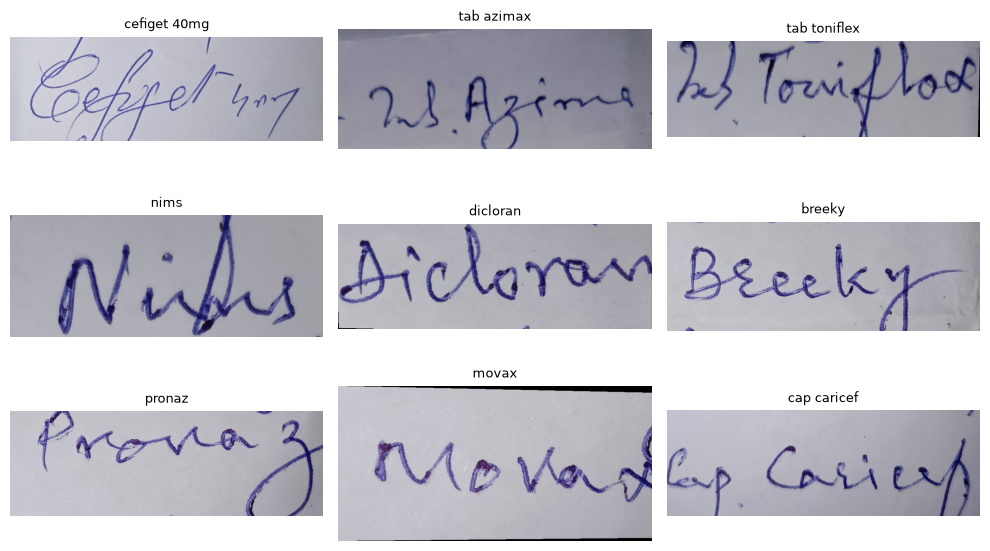
\includegraphics[width=.88\linewidth,height=5cm,keepaspectratio]{labs/visuals/06-notebook-reference.png}
\end{labvisual}
\begin{refoutput}
\begin{lstlisting}[style=utpterminal]
Labelled images: 89 | unique labels: 61
\end{lstlisting}
\end{refoutput}

\textbf{What it means.} One label file and 89 photographs, each present exactly once. The 89 labels hold 61 distinct medicine names, so some names appear several times in different handwriting. The grid shows what the engine faces: cursive, varied stroke width, uneven lighting and lined paper.
\end{labanswer}

\begin{labquestion}{2}{Run the baseline OCR}
Use one fixed Tesseract configuration for every raw image (LSTM engine, page-segmentation mode 7 = one text line) and normalise both prediction and label to lowercase letters and digits. Record a per-image engine failure instead of dropping the sample or stopping the benchmark.
\end{labquestion}
\begin{labanswer}
\lstinputlisting[style=utppython,firstline=66,lastline=102]{all_experiments/lab06_handwriting_ocr_worked.py}
\begin{refoutput}
\begin{lstlisting}[style=utpterminal]
          truth      prediction prediction_norm
0  cefiget 40mg
1    tab azimax              Ao              ao
2  tab toniflex  p53 Towid host    p53towidhost
3          nims            Nidu            nidu
4      dicloran        diclerew        diclerew
OCR engine errors: 0
\end{lstlisting}
\end{refoutput}

\textbf{What it means.} The first rows distinguish a blank recognition from a misread name while retaining every labelled image. The configuration is fixed, so any later improvement must come from the image rather than from engine tuning.
\end{labanswer}

\textbf{Connect it to the chapter.} The next questions measure the second and third boxes of this pipeline, and an error made in the first cannot be repaired by them.
% Reused from chapters/06-nlp-foundations.tex
\begin{labvisual}{Recall the chapter model}
\begin{labgraphic}
\begin{tikzpicture}[scale=0.99,transform shape,
  b/.style={draw=UTPBlue,fill=UTPPaleBlue,rounded corners=2mm,minimum width=2.20cm,minimum height=1.0cm,align=center,font=\small\color{UTPNavy}},
  arr/.style={-{Stealth[length=2mm]},thick,draw=UTPTeal}
]
\node[b] (acq) {Acquire\\\scriptsize photo, audio, keyboard};
\node[b,right=0.26cm of acq] (norm) {Normalise\\\scriptsize case, punctuation, tokens};
\node[b,right=0.26cm of norm] (rep) {Represent\\\scriptsize counts, n-grams, vectors};
\node[b,right=0.26cm of rep] (model) {Model\\\scriptsize classify, translate, search};
\node[b,right=0.26cm of model] (eval) {Evaluate\\\scriptsize against references};
\draw[arr] (acq)--(norm); \draw[arr] (norm)--(rep); \draw[arr] (rep)--(model); \draw[arr] (model)--(eval);
\draw[utpbrace,decoration={mirror},draw=UTPOrange] (-1.3,-0.75) -- (3.9,-0.75);
\node[font=\scriptsize\color{UTPOrange},anchor=north] at (1.3,-0.95) {Lab~6: OCR, normalisation, measurement};
\draw[utpbrace,decoration={mirror},draw=UTPGreen] (4.1,-0.75) -- (12.0,-0.75);
\node[font=\scriptsize\color{UTPGreen},anchor=north] at (8.1,-0.95) {Lab~7: bag of words, Naive Bayes, evaluation};
\end{tikzpicture}
\end{labgraphic}\end{labvisual}


\begin{labquestion}{3}{Measure recognition quality}
Implement Levenshtein edit distance and report, for the baseline: exact-match accuracy, mean normalised edit distance (distance divided by the longer string, so it lies in 0--1), character error rate (total edits divided by total reference characters; it can exceed 1), and the number of blank predictions.
\end{labquestion}
\begin{labanswer}
Inspect the normalisation and distance functions before interpreting the metrics:
\courselabtrace{Trace the OCR scoring fields}{1. Input / state}{Keep each filename, reference and prediction together; normalise both strings consistently.}{2. Operation}{add\_distances computes exact match and edit distances for each row; summarise aggregates the scored rows.}{3. Check}{Blank predictions remain failures. Compare baseline and preprocessed on the same labelled images.}


\lstinputlisting[style=utppython,firstline=104,lastline=133]{all_experiments/lab06_handwriting_ocr_worked.py}
\begin{refoutput}
\begin{lstlisting}[style=utpterminal]
   pipeline  exact_match  mean_norm_edit_distance  character_error_rate  blank_predictions
0  baseline        0.000                   0.8598                0.8805                 44
\end{lstlisting}
\end{refoutput}

\textbf{What it means.} Generic OCR on raw handwriting is poor: none of the 89 names is read exactly, the character error rate is close to 0.9, and 44 images yield no text. Any engine error is counted as a failed recognition, not silently removed.
\end{labanswer}

\begin{labquestion}{4}{Build one preprocessing pipeline}
Convert each image to grayscale, add a 20-pixel white border, cap the width at 1,200 pixels, and enlarge by $1.5\times$ with bicubic resampling. Save the results under \texttt{results/lab06/preprocessed/}. The OCR configuration does not change.
\end{labquestion}
\begin{labanswer}
\lstinputlisting[style=utppython,firstline=135,lastline=148]{all_experiments/lab06_handwriting_ocr_worked.py}
\begin{refoutput}
\begin{lstlisting}[style=utpterminal]
Prepared images: 89 | example size: (1800, 638) mode: L
\end{lstlisting}
\end{refoutput}

\textbf{What it means.} Each step targets a known weakness of Tesseract on photographs: grayscale removes colour noise, the border stops text touching the edge (which breaks line segmentation), the width cap bounds runtime, and the enlargement brings stroke height into the range the engine was trained on. Only the image changes.
\end{labanswer}

\begin{labquestion}{5}{Compare the two pipelines fairly}
Run OCR on the preprocessed images with the identical configuration, keep exactly the same 89 samples, save one row per image and pipeline to \texttt{predictions.csv}, and save both sets of metrics to \texttt{metrics.csv}.
\end{labquestion}
\begin{labanswer}
\lstinputlisting[style=utppython,firstline=150,lastline=156]{all_experiments/lab06_handwriting_ocr_worked.py}
\begin{refoutput}
\begin{lstlisting}[style=utpterminal]
                         exact_match  mean_norm_edit_distance    CER  blank
baseline                      0.0000                   0.8598  0.8805     44
grayscale_border_resize       0.0112                   0.7673  0.7883     15
\end{lstlisting}
\end{refoutput}

\textbf{What it means.} Preprocessing cuts the blank predictions from 44 to 15 and lowers the character error rate by about 0.09, but exact-match accuracy barely moves (one correct name out of 89): the engine now \emph{sees} text on most images yet still cannot read cursive. Because both pipelines were scored on the same 89 images with the same configuration, the difference is attributable to the preprocessing alone. Exact numbers depend on the Tesseract version; the direction of the changes should not.
\end{labanswer}

\begin{labquestion}{6}{Analyse the failures}
Take the worst preprocessed predictions by normalised edit distance and tag each as an \emph{engine error}, \emph{no text detected}, or \emph{character confusion}. Save \texttt{error\_analysis.csv} and a figure of the six hardest images.
\end{labquestion}
\begin{labanswer}
\lstinputlisting[style=utppython,firstline=158,lastline=174]{all_experiments/lab06_handwriting_ocr_worked.py}
\begin{refoutput}
\begin{lstlisting}[style=utpterminal]
Saved: ['error_analysis.csv', 'metrics.csv', 'ocr_failures.png', 'predictions.csv', 'sample_grid.png']
\end{lstlisting}
\end{refoutput}

\textbf{What it means.} Of the eight worst cases, seven are \emph{no text detected} and one is \emph{character confusion}. An engine error is a recorded runtime failure, no text detected is a segmentation failure, and character confusion is a recognition failure, and each needs a different fix. This is a benchmark of how well a model fits a domain, not evidence that generic OCR suits clinical transcription.
\end{labanswer}

\begin{yourturn}
Add new cells at the end of the notebook. Tasks 1 and 2 work in live and cached mode, because they recompute from the saved predictions. Task 3 needs live OCR.
\begin{enumerate}
  \item \textbf{Look past the totals.} Using \texttt{baseline} and \texttt{preprocessed}, count the images whose edits improved, worsened or stayed the same, and how many went from blank to text and from text to blank.
  \item \textbf{Change the normaliser.} Recompute CER for both pipelines with a normaliser that keeps single spaces, and again with no normalisation at all. How much of the ``error'' depends on this rule?
  \item \textbf{Test one more step (live mode only).} Add one preprocessing step of your own, for example \texttt{ImageOps.autocontrast}. Keep the images, labels, normaliser and OCR configuration fixed, and report whether blanks and CER move. Keep your result whichever way it goes: a step that does not help is still a finding.
\end{enumerate}
\begin{lstlisting}[style=utppython]
b, p = baseline.set_index("filename"), preprocessed.set_index("filename")
print("improved", (p.edits < b.edits).sum(), "worse", (p.edits > b.edits).sum(), "same", (p.edits == b.edits).sum())
print("blank to text", ((b.prediction_norm == "") & (p.prediction_norm != "")).sum(),
      "text to blank", ((b.prediction_norm != "") & (p.prediction_norm == "")).sum())
\end{lstlisting}
\end{yourturn}

\begin{expectedfindings}
\begin{enumerate}
  \item On the saved predictions: 43 improved, 18 worse and 28 the same; 34 went from blank to text and 5 from text to blank. \texttt{tab mesulid}, for example, was read as \texttt{wos Mesulia} on the raw image and not at all after preprocessing. The aggregate improvement hides real losses.
  \item Keeping spaces gives CER 0.884 (baseline) and 0.783 (preprocessed). No normalisation gives 0.928 and 0.858. The ordering of the pipelines survives, and the gap between them does not stay the same, so always state the rule.
  \item This depends on your Tesseract version and your choice of step, so there is no fixed answer. Your report should give the numbers for all three pipelines on the same 89 images.
\end{enumerate}
\end{expectedfindings}

\begin{troubleshoot}
\begin{description}
  \item[\texttt{tesseract is not recognized}] Close and reopen the terminal after installing, or add the install folder to \texttt{PATH}. The notebook will still find the default Windows location.
  \item[The first line says \texttt{cached} after installing] Restart the Jupyter kernel so it sees the new program, and check that \texttt{pytesseract} is installed in the active environment.
  \item[\texttt{predictions.csv is missing} in cached mode] Restore \texttt{results/lab06/predictions.csv} from the course package, or install Tesseract.
  \item[Slightly different numbers in live mode] Expected: Tesseract versions differ. Report your version with your numbers.
\end{description}
\end{troubleshoot}

\begin{verification}
\begin{itemize}
  \item All 89 labelled images are present exactly once.
  \item Both pipelines are scored on the same 89 images with the identical OCR configuration, and engine failures are counted, not dropped.
  \item Exact match, normalised edit distance, character error rate and blank predictions are reported for both pipelines.
  \item Preprocessing reduces the blank predictions (from 44 to 15 on the saved run), and you can explain why exact match barely moves.
  \item \texttt{results/lab06/} holds \texttt{predictions.csv}, \texttt{metrics.csv}, \texttt{error\_analysis.csv}, \texttt{sample\_grid.png} and \texttt{ocr\_failures.png}.
\end{itemize}
\end{verification}

\begin{labdeliverable}
\begin{itemize}
  \item Restart the kernel and run all cells without errors.
  \item Submit the executed notebook, including your \emph{Your turn} cells, and the generated \texttt{results/lab06/} folder.
  \item Report the OCR mode and, for a live run, the Tesseract version.
  \item State which OCR stage improved, which failure remained, and why this pipeline is not suitable for autonomous clinical transcription.
\end{itemize}
\end{labdeliverable}

\chapter{NLP Methods: Text Classification Done Honestly}
\label{ch:nlp-methods}

\chapterguide%
  {Know the NLP pipeline of \chapref{ch:nlp-foundations}, basic probability, and what precision, recall and F1 measure.}
  {turn tweets into a bag-of-words matrix; explain how Multinomial Naive Bayes scores a class and why smoothing is needed; choose metrics for imbalanced classes; run a leakage-safe train/validation/test protocol; and read a confusion matrix, a per-group table and an error sample as evidence.}

Lab~7 classifies airline tweets as negative, neutral or positive using Multinomial Naive Bayes on word counts. The model is deliberately simple, because the focus here is the evaluation protocol: prepare text without leakage, tune on validation data, report metrics that respect imbalance, and inspect the errors. The same protocol applies to much larger models.

\section{From text to numbers}

A classifier needs numbers, and a tweet is a string. The simplest bridge is a \term{bag of words}: represent each document by how many times each vocabulary term occurs in it, and throw away the word order.

\begin{analogy}
Tip a tweet's words into a bag and shake it. You can still count them, and ``cancelled'' appearing three times tells you a good deal about the mood. You can no longer tell ``not good, very bad'' from ``not bad, very good''. That lost order is the price of this representation, and it is why this chapter ends by asking what to try next.
\end{analogy}

\begin{utpfig}[The text preprocessing pipeline]{One tweet through Lab~7's preprocessing. Placeholders stand in for the handle and the link, and then the tokeniser and the stop-word list do their work. ``Again'' is on scikit-learn's English stop list, so it disappears, as do ``not'', ``no'' and ``never'' in other tweets.}{fig:preprocess}
\begin{tikzpicture}[
  stage/.style={utpbox,text width=2.7cm,minimum height=1.05cm,
    font=\scriptsize\ttfamily\color{UTPNavy}},
  stagelabel/.style={utplabel,anchor=north,align=center,text width=2.7cm}
]
\node[stage] (raw) {@united Flight\\cancelled AGAIN!\\http://t.co/x};
\node[stage,right=0.6cm of raw] (normalized) {user flight\\cancelled again!\\url};
\node[stage,right=0.6cm of normalized] (filtered) {user flight\\cancelled url};
\node[stage,right=0.6cm of filtered,fill=UTPPaleTeal,draw=UTPGreen]
  (counts) {cancelled:1\ flight:1\\url:1\ user:1};
\draw[utparrow] (raw.east) -- (normalized.west);
\draw[utparrow] (normalized.east) -- (filtered.west);
\draw[utparrow] (filtered.east) -- (counts.west);
\node[stagelabel] at ([yshift=-2mm]raw.south) {Raw tweet};
\node[stagelabel] at ([yshift=-2mm]normalized.south) {Replace handles and\\URLs, lowercase};
\node[stagelabel] at ([yshift=-2mm]filtered.south) {Tokenise, drop\\stop words};
\node[stagelabel] at ([yshift=-2mm]counts.south) {Count terms\\(the bag of words)};
\end{tikzpicture}
\end{utpfig}

Lab~7's \texttt{clean} function replaces URLs and handles with the placeholders \texttt{URL} and \texttt{USER} and then lowercases everything, so they become the single features \texttt{url} and \texttt{user} rather than thousands of one-off terms. \texttt{CountVectorizer} then tokenises, removes English stop words, requires a term to occur in at least two training tweets, and caps the vocabulary at 20,000.

\subsection{N-grams}

\term{Bigrams} add pairs of adjacent tokens as extra features, which brings back a little of the lost word order. Pairs such as \texttt{hold hours}, \texttt{great flight} and \texttt{best airline} turn up among the most class-specific features in Lab~7. Features grow from 4,671 to 11,850, and the matrix becomes sparser, so let validation performance decide whether they help.

\section{Multinomial Naive Bayes}

Naive Bayes chooses the class $c$ that makes the document $d$ most probable:
\[
\hat c=\argmax_c\; P(c)\prod_{w\in d}P(w\mid c)^{n_w},
\]
where $n_w$ counts term $w$ in the document, $P(c)$ is the class's share of the training set, and $P(w\mid c)$ is how often term $w$ appears among that class's words. The ``naive'' part is the assumption that terms are independent once the class is known. That is plainly false for language, and the model works usefully anyway.

\begin{intuition}
Think of every word as a witness giving evidence. ``Delayed'' testifies strongly for negative, ``thanks'' testifies for positive, and ``flight'' says about the same to everyone, so it barely matters. Naive Bayes multiplies the testimony together, starting from how common each class is, and the largest product wins.
\end{intuition}

\figref{fig:naive-bayes} scores two short tweets with the probabilities the fitted Lab~7 model actually learned. Notice the second tweet. Positive tweets are only 16\,\% of the data, so the model starts sceptical, but ``great'' and ``thanks'' are strong enough evidence to overturn that.

\begin{utpfig}[How Naive Bayes scores a sentence]{Two short messages scored with single-word probabilities from the fitted Lab~7 model. Each class starts from its share of the training set and multiplies in one probability per word. ``Flight'' contributes much the same to every class; the other words do the deciding. The largest score in each row is the prediction.}{fig:naive-bayes}
\begin{tikzpicture}[font=\small,
  head/.style={utpcell,minimum width=1.3cm,minimum height=0.55cm,font=\scriptsize\bfseries\color{UTPNavy}},
  val/.style={minimum width=1.3cm,minimum height=0.5cm,draw=#1!55,fill=#1!10,font=\scriptsize\color{UTPNavy},inner sep=0pt},
  cl/.style={utplabel,anchor=east,font=\scriptsize\bfseries},
  score/.style={utplabel,anchor=west,font=\scriptsize\color{UTPNavy}}]
\def\tw{1.4}
\node[utplabel,anchor=east,color=UTPNavy] at (-0.95,1.75) {\textbf{tweet 1}};
\foreach \h/\i in {share/0,flight/1,delayed/2,hold/3}{\node[head] at (\tw*\i,1.75) {\h};}
\foreach \v/\i in {0.635/0,0.0235/1,0.00393/2,0.00483/3}{\node[val=UTPRed] at (\tw*\i,1.15) {\v};}
\foreach \v/\i in {0.209/0,0.0175/1,0.00067/2,0.00067/3}{\node[val=UTPMuted] at (\tw*\i,0.6) {\v};}
\foreach \v/\i in {0.156/0,0.0129/1,0.00062/2,0.00022/3}{\node[val=UTPGreen] at (\tw*\i,0.05) {\v};}
\node[cl,color=UTPRed] at (-0.75,1.15) {negative};
\node[cl,color=UTPMuted] at (-0.75,0.6) {neutral};
\node[cl,color=UTPGreen] at (-0.75,0.05) {positive};
\node[score] at (5.0,1.15) {$=2.8\times10^{-7}$\quad\textbf{predicted: negative}};
\node[score] at (5.0,0.6) {$=1.6\times10^{-9}$};
\node[score] at (5.0,0.05) {$=2.7\times10^{-10}$};
\begin{scope}[yshift=-2.75cm]
\node[utplabel,anchor=east,color=UTPNavy] at (-0.95,1.75) {\textbf{tweet 2}};
\foreach \h/\i in {share/0,great/1,flight/2,thanks/3}{\node[head] at (\tw*\i,1.75) {\h};}
\foreach \v/\i in {0.635/0,0.00066/1,0.0235/2,0.00259/3}{\node[val=UTPRed] at (\tw*\i,1.15) {\v};}
\foreach \v/\i in {0.209/0,0.00047/1,0.0175/2,0.00406/3}{\node[val=UTPMuted] at (\tw*\i,0.6) {\v};}
\foreach \v/\i in {0.156/0,0.00839/1,0.0129/2,0.0203/3}{\node[val=UTPGreen] at (\tw*\i,0.05) {\v};}
\node[cl,color=UTPRed] at (-0.75,1.15) {negative};
\node[cl,color=UTPMuted] at (-0.75,0.6) {neutral};
\node[cl,color=UTPGreen] at (-0.75,0.05) {positive};
\node[score] at (5.0,1.15) {$=2.6\times10^{-8}$};
\node[score] at (5.0,0.6) {$=7.0\times10^{-9}$};
\node[score] at (5.0,0.05) {$=3.4\times10^{-7}$\quad\textbf{predicted: positive}};
\end{scope}
\end{tikzpicture}
\end{utpfig}

\subsection{Smoothing}

What if a word never occurred in any training tweet of some class? Its probability is zero, and one zero wipes out the whole product, however strongly the other words point that way. One unfamiliar witness silences everyone. \term{Laplace smoothing} prevents this by adding a small pseudo-count $\alpha$ to every term, as if each word had been seen a tiny number of times in every class:
\[
P(w\mid c)=\frac{\text{count}(w,c)+\alpha}{\sum_{w'}\text{count}(w',c)+\alpha\,|V|}.
\]
Small $\alpha$ trusts the observed counts, and large $\alpha$ moves the probabilities towards uniform. Multiplying many small numbers also underflows a computer's floating point, so real implementations add logarithms instead. Lab~7 selects $\alpha=0.3$ from $\{0.3,0.5,1,2\}$ on validation data, and n-grams turn out to matter more than smoothing here.

\section{Metrics for imbalanced classes}

Tweets are 63\,\% negative, 21\,\% neutral and 16\,\% positive. A model that always says ``negative'' scores 63\,\% accuracy while being completely useless, so accuracy cannot be the headline. Report per-class metrics as well:

\begin{utptable}
\begin{tabularx}{\linewidth}{@{}>{\bfseries\leavevmode\color{UTPNavy}}m{0.16\linewidth}m{0.36\linewidth}X@{}}
\toprule
\rowcolor{UTPPaleBlue!92}
\utpth{Metric} & \utpth{Definition} & \utpth{Answers} \\
\midrule
Precision & Of the tweets predicted as class $c$, the fraction that are $c$ & When the model says positive, how often is it right? \\
Recall & Of the tweets that are $c$, the fraction predicted as $c$ & How many of the positive tweets did it find? \\
F1 & Harmonic mean of precision and recall & One number per class that punishes neglecting either \\
\bottomrule
\end{tabularx}
\end{utptable}

\figref{fig:nb-confusion} shows where these come from on the real test set. \term{Macro F1} is the plain average of the three class F1 scores, so each class counts equally however rare it is. The majority baseline has recall~1 for negative and~0 otherwise, giving macro F1 $0.26$; Naive Bayes reaches $0.70$.

\begin{utpfig}[The Naive Bayes confusion matrix]{Lab~7's test results on 2,143 tweets. For \emph{neutral}: recall reads along its row, $239/447=0.53$, and precision reads down its column, $239/400=0.60$. Their harmonic mean is F1 $=0.56$. The largest off-diagonal cell, 158, is neutral tweets called negative.}{fig:nb-confusion}
\begin{tikzpicture}[font=\small,
  hit/.style={draw=UTPGreen,fill=UTPGreen!28,minimum width=1.75cm,minimum height=0.74cm,font=\small\bfseries\color{UTPNavy}},
  miss/.style={draw=UTPMuted!30,fill=white,minimum width=1.75cm,minimum height=0.74cm,font=\small\color{UTPMuted}},
  bad/.style={draw=UTPOrange,fill=UTPPaleOrange,minimum width=1.75cm,minimum height=0.74cm,font=\small\bfseries\color{UTPNavy}}]
\def\cw{1.8}\def\ch{0.78}
\foreach \name [count=\i from 0] in {negative,neutral,positive}{\node[font=\scriptsize\color{UTPNavy},anchor=south,align=center] at (\cw*\i,0.42) {predicted\\\name};}
\foreach \name [count=\i from 0] in {negative,neutral,positive}{\node[font=\scriptsize\color{UTPNavy},anchor=east] at (-1.0,-\ch*\i) {true \name};}
\node[hit] at (0,0) {1185};\node[miss] at (\cw,0) {115};\node[miss] at (2*\cw,0) {61};
\node[bad] at (0,-\ch) {158};\node[hit] at (\cw,-\ch) {239};\node[miss] at (2*\cw,-\ch) {50};
\node[miss] at (0,-2*\ch) {63};\node[miss] at (\cw,-2*\ch) {46};\node[hit] at (2*\cw,-2*\ch) {226};
\node[anchor=west,align=left,text width=5.2cm,font=\scriptsize\color{UTPNavy}] at (2*\cw+1.3,-\ch) {\textbf{Per-class F1}\\[2pt] negative $0.86$\\ neutral $0.56$\\ positive $0.67$\\[3pt] macro F1 $=(0.86+0.56+0.67)/3=0.70$};
\end{tikzpicture}
\end{utpfig}

\begin{pitfall}
Compute the majority baseline first. Accuracy rises from 63\,\% to 77\,\%, which sounds modest, while macro F1 rises from $0.26$ to $0.70$. Together they show what the model adds.
\end{pitfall}

\section{A leakage-safe protocol}

\term{Leakage} occurs when test information influences training or model selection. It is the examination equivalent of seeing the final paper in advance: the score goes up and tells you nothing about what you can do on a new paper. Lab~7 controls leakage at each stage (\figref{fig:protocol}).

\begin{utpfig}[The evaluation protocol of Lab~7]{Deduplicate before splitting, fit vocabulary and model on training data, select settings on validation data, and evaluate once on test data.}{fig:protocol}
\begin{tikzpicture}[font=\small,
  s/.style={utpbox,minimum width=2.6cm,minimum height=1.0cm,font=\scriptsize\color{UTPNavy},align=center}]
\node[s] (dedup) at (0,0) {\textbf{1. Deduplicate}\\exact and normalised\\copies removed};
\node[s,right=0.45cm of dedup] (split) {\textbf{2. Split 70/15/15}\\stratified, seed 42\\saved to split.csv};
\node[s,right=0.45cm of split,fill=UTPPaleOrange,draw=UTPOrange] (fit) {\textbf{3. Fit on train}\\vocabulary and\\Naive Bayes};
\node[s,right=0.45cm of fit,fill=UTPPaleOrange,draw=UTPOrange] (tune) {\textbf{4. Tune on validation}\\n-grams and $\alpha$\\by macro F1};
\node[s,right=0.45cm of tune,fill=UTPPaleTeal,draw=UTPGreen] (test) {\textbf{5. Test once}\\metrics, confusion\\matrix, errors};
\foreach \a/\b in {dedup/split, split/fit, fit/tune, tune/test}{\draw[utparrow] (\a)--(\b);}
\node[utplabel,anchor=north,color=UTPOrange] at (7.05,-0.75) {sees training and validation rows only};
\node[utplabel,anchor=north,color=UTPGreen] at (11.9,-0.75) {sees test rows: once};
\end{tikzpicture}
\end{utpfig}

\begin{description}
  \item[Duplicates before the split.] There are 213 exact duplicates and 355 duplicates after URL and mention replacement. Keep one copy of each normalised text before splitting, or a retweet in the training set could hand the model the answer to its twin in the test set.
  \item[Stratified, seeded, saved.] Preserve class proportions in a seeded 70/15/15 split and save the assignment for audit.
  \item[Vocabulary from training text only.] Fit \texttt{CountVectorizer} on training tweets, then transform validation and test tweets. Words seen only in the test set stay unknown, exactly as they would for a deployed model.
  \item[Selection on validation, one look at test.] Compare eight settings on validation data, refit the winner, then evaluate once on test data.
\end{description}

\begin{keyidea}
Deduplicate, split, fit, tune, test. Respecting these boundaries keeps the final score separate from model development.
\end{keyidea}

\section{Reading the evidence}

The lab produces four kinds of evidence, each answering a question the headline score cannot.

\begin{description}
  \item[The confusion matrix.] Neutral tweets are often predicted as negative, because questions about delays share vocabulary with complaints.
  \item[Per-class scores.] Negative F1 $0.86$, positive $0.67$, neutral $0.56$. Neutral is the hardest class, with few distinctive words of its own. Its most class-specific features are one-off news topics such as \texttt{wall street} and \texttt{journal}, which say little about any future tweet.
  \item[Per-group scores.] Airline macro F1 ranges from $0.66$ to $0.78$, with 63--594 test tweets per airline. Different sample sizes, class mixes and topics make this a diagnostic, not an airline ranking.
  \item[An error sample.] Tag the four most confident mistakes per true class, twelve tweets in all. The reproducible sample reveals missed negation, low-sentiment questions, short texts and a repeatedly retweeted joke with inconsistent labels. The last is a data-quality issue, not just a model error.
\end{description}

\begin{pitfall}
Every sampled error has posterior above $0.999$. Being confident and wrong is the most damaging kind of mistake, and Naive Bayes does it often because its independence assumption multiplies correlated evidence as if it were new each time. Use these scores for ranking, not as reliable probabilities of being right.
\end{pitfall}

\section{What the protocol does not fix}

Bag-of-words Naive Bayes struggles with negation, sarcasm and word order, and one choice in this pipeline makes that worse. The English stop list removes \texttt{not}, \texttt{no} and \texttt{never}, so ``not good'' and ``good'' look identical. Keeping stop words raises validation macro F1 from $0.697$ to $0.720$ with the same model. That is a real finding, and it came from questioning a default rather than from a more complicated model. The deliverable asks what representation to try next: weighted counts, embeddings or contextual models. Whatever you try, keep the deduplicated split, validation-based selection and single final test evaluation unchanged.

\begin{chapterrecap}
\begin{itemize}
  \item A bag of words counts terms and discards order; bigrams recover a little of it.
  \item Naive Bayes multiplies a class's share by one probability per word, and smoothing stops one unseen word from zeroing a class.
  \item On imbalanced classes, compare macro F1 against a majority baseline and read the confusion matrix.
  \item Deduplicate, split, fit on train, tune on validation and test once. Anything else leaks.
  \item Confidence is not correctness, and defaults such as the stop list deserve testing too.
\end{itemize}
\end{chapterrecap}

\begin{quickcheck}
\begin{enumerate}
  \item Why are URLs and \texttt{@handles} replaced by placeholder tokens rather than deleted or kept?
  \item A term appears 0 times in the positive training tweets. What happens to a tweet containing it under Naive Bayes without smoothing, and with $\alpha=1$?
  \item The majority baseline scores 63\,\% accuracy and 0.26 macro F1. Explain both numbers from the class shares alone.
  \item Which step would leak if the vectoriser were fitted on all 14,285 tweets, and what would the symptom be?
  \item Virgin America has the highest per-airline macro F1 and only 63 test tweets. Why does the lab warn against reading this as an airline ranking?
\end{enumerate}
\end{quickcheck}

\labsection{7}{NLP Evaluation: Airline Tweet Sentiment Classification}{sec:lab07-nlp-b}

\begin{labproject}{Build and evaluate a three-class sentiment classifier}
\textbf{Read first.} Chapter~\ref{ch:nlp-methods}.\\
\textbf{Goal.} Compare a majority baseline with validation-tuned Multinomial Naive Bayes under a leakage-safe protocol.\\
\textbf{Scenario.} An airline support team wants to classify customer tweets as negative, neutral or positive.\\
\textbf{Data.} \texttt{all\_datasets/lab07-Tweets.csv} (14,640 tweets about six US airlines).\\
\textbf{Notebook.} \texttt{all\_experiments/lab07\_airline\_sentiment\_worked.ipynb}.\\
\textbf{Hand in.} The executed notebook, the \texttt{results/lab07/} folder and a short conclusion, as listed in the checklist at the end of this sheet.
\end{labproject}

\begin{labmode}
\begin{enumerate}
  \item Activate your course environment and confirm that the data file is in \texttt{all\_datasets/}.
  \item Start Jupyter from \texttt{all\_experiments/}, open the notebook, and choose \textbf{Restart Kernel and Run All Cells}. Everything runs in a few seconds.
\end{enumerate}
\begin{lstlisting}[style=utpterminal]
cd all_experiments
jupyter lab
\end{lstlisting}
Prefer a plain script? From the course folder, \texttt{python all\_experiments/lab07\_airline\_sentiment\_worked.py} runs the same code and writes the same evidence.
\end{labmode}

\courselabflow{Clean tweets}{Split data}{Tune pipeline}{Test once}


\labroutine

\begin{yourturn}
\textbf{Warm-up on paper.} The figures of Chapter~\ref{ch:nlp-methods} give two tweets scored by hand. Repeat the idea for the two-word message \emph{delayed thanks}, using negative: share 0.635, delayed 0.00393, thanks 0.00259; positive: share 0.156, delayed 0.00062, thanks 0.0203. Which class wins?

\emph{Answer.} Negative: $0.635\times0.00393\times0.00259\approx6.5\times10^{-6}$. Positive: $0.156\times0.00062\times0.0203\approx2.0\times10^{-6}$. Negative wins, because ``delayed'' and the class share together outweigh ``thanks''.
\end{yourturn}

\textbf{Setup.} Run the imports and path setup first, and keep this kernel state for the later questions. In the script version the first seven lines also set the working directory.
\lstinputlisting[style=utppython,firstline=1,lastline=7]{all_experiments/lab07_airline_sentiment_worked.py}
\lstinputlisting[style=utppython,firstline=8,lastline=24]{all_experiments/lab07_airline_sentiment_worked.py}

\begin{labquestion}{1}{Inspect and clean the data}
Keep tweet id, text, sentiment and airline. Report the class balance and the number of duplicate texts. Replace URLs and \texttt{@mentions} with placeholder tokens, then drop duplicates \emph{before} splitting, both exact copies and tweets that become identical after normalisation, so that no near-copy can land in two different subsets.
\end{labquestion}
\begin{labanswer}
\courselabtrace{Vocabulary belongs to training data}{Train}{Learn vocabulary and class probabilities}{Validation}{Select smoothing with fixed features}{Test}{Report macro F1 and the confusion matrix}

\lstinputlisting[style=utppython,firstline=26,lastline=40]{all_experiments/lab07_airline_sentiment_worked.py}
\begin{refoutput}
\begin{lstlisting}[style=utpterminal]
Raw tweets: 14640 | exact duplicate texts: 213
Duplicates after normalisation: 355
Tweets kept: 14285
share:  negative 0.635   neutral 0.209   positive 0.156
\end{lstlisting}
\end{refoutput}

\textbf{What it means.} 14,640 tweets shrink to 14,285 after duplicate handling. Negative tweets are 63\,\% of the data, so a classifier that always says \emph{negative} would score 63\,\% accuracy while being useless, and macro F1 is therefore the headline metric. Removing near-duplicates before the split matters: a retweet in the training set and its twin in the test set would inflate every score.
\end{labanswer}

\begin{labquestion}{2}{Create a fixed stratified split}
Split 70/15/15 with seed 42, stratified by sentiment, and save tweet ids with their split label to \texttt{split.csv}.
\end{labquestion}
\begin{labanswer}
\lstinputlisting[style=utppython,firstline=42,lastline=49]{all_experiments/lab07_airline_sentiment_worked.py}
\begin{refoutput}
\begin{lstlisting}[style=utpterminal]
split       negative  neutral  positive    All
test            1361      447       335   2143
train           6348     2087      1564   9999
validation      1360      447       336   2143
\end{lstlisting}
\end{refoutput}

\textbf{What it means.} Stratification keeps the 63/21/16 class mix in all three subsets. The test subset is now frozen: nothing below looks at it until Question~6.
\end{labanswer}

\begin{labquestion}{3}{Fit text features on training data only}
Build a bag of words with \texttt{CountVectorizer} (English stop words removed, terms in fewer than two training tweets dropped, at most 20,000 features). Fit it on the training texts only and report the vocabulary size for unigrams and for unigrams plus bigrams.
\end{labquestion}
\begin{labanswer}
The vocabulary is itself something learned from training data. Trace how it moves through the protocol:
\courselabtrace{Trace fit versus transform in text classification}{1. Input / state}{Clean and deduplicate model\_text, then preserve train, val and test indices.}{2. Operation}{Fit a vectorizer on model\_text[train]; transform other splits using those learned feature columns.}{3. Check}{After validation selects settings, features transforms test text and model predicts X\_test.}


\lstinputlisting[style=utppython,firstline=51,lastline=57]{all_experiments/lab07_airline_sentiment_worked.py}
\begin{refoutput}
\begin{lstlisting}[style=utpterminal]
ngram_range=(1, 1): 4,671 features
ngram_range=(1, 2): 11,850 features
\end{lstlisting}
\end{refoutput}

\textbf{What it means.} The vocabulary is learned from training tweets alone, so a word that appears only in validation or test tweets is unknown to the model, exactly the situation a deployed classifier faces. Adding bigrams more than doubles the vocabulary and lets the model see phrases such as \emph{hold hours} and \emph{great flight} that a unigram model splits apart.
\end{labanswer}

\textbf{Connect it to the chapter.} This is what \texttt{clean} and the vectoriser do to one tweet. Notice what has gone by the last step.
% Reused from chapters/08-nlp-methods.tex
\begin{labvisual}{Recall the chapter model}
\begin{labgraphic}
\begin{tikzpicture}[
  stage/.style={utpbox,text width=2.7cm,minimum height=1.05cm,
    font=\scriptsize\ttfamily\color{UTPNavy}},
  stagelabel/.style={utplabel,anchor=north,align=center,text width=2.7cm}
]
\node[stage] (raw) {@united Flight\\cancelled AGAIN!\\http://t.co/x};
\node[stage,right=0.6cm of raw] (normalized) {user flight\\cancelled again!\\url};
\node[stage,right=0.6cm of normalized] (filtered) {user flight\\cancelled url};
\node[stage,right=0.6cm of filtered,fill=UTPPaleTeal,draw=UTPGreen]
  (counts) {cancelled:1\ flight:1\\url:1\ user:1};
\draw[utparrow] (raw.east) -- (normalized.west);
\draw[utparrow] (normalized.east) -- (filtered.west);
\draw[utparrow] (filtered.east) -- (counts.west);
\node[stagelabel] at ([yshift=-2mm]raw.south) {Raw tweet};
\node[stagelabel] at ([yshift=-2mm]normalized.south) {Replace handles and\\URLs, lowercase};
\node[stagelabel] at ([yshift=-2mm]filtered.south) {Tokenise, drop\\stop words};
\node[stagelabel] at ([yshift=-2mm]counts.south) {Count terms\\(the bag of words)};
\end{tikzpicture}
\end{labgraphic}\end{labvisual}


\begin{labquestion}{4}{Establish a majority-class baseline}
Predict the most frequent training class for every validation tweet and record its accuracy and macro F1. Any real model must beat this.
\end{labquestion}
\begin{labanswer}
\lstinputlisting[style=utppython,firstline=59,lastline=62]{all_experiments/lab07_airline_sentiment_worked.py}
\begin{refoutput}
\begin{lstlisting}[style=utpterminal]
Majority class: negative | validation accuracy 0.635 | validation macro F1 0.259
\end{lstlisting}
\end{refoutput}

\textbf{What it means.} The majority baseline reaches 63\,\% accuracy but only 0.26 macro F1, because its recall on \emph{neutral} and \emph{positive} is zero. This is the number that shows why accuracy alone misleads on imbalanced classes.
\end{labanswer}

\begin{labquestion}{5}{Tune Naive Bayes on validation data}
Grid-search the n-gram range $\{(1,1), (1,2)\}$ and the smoothing parameter $\alpha \in \{0.3, 0.5, 1, 2\}$, scoring by validation macro F1. Save \texttt{validation\_results.csv} and select the best setting without looking at the test data.
\end{labquestion}
\begin{labanswer}
\lstinputlisting[style=utppython,firstline=64,lastline=79]{all_experiments/lab07_airline_sentiment_worked.py}
\begin{refoutput}
\begin{lstlisting}[style=utpterminal]
ngram_range  alpha  validation_macro_f1
(1, 2)         0.3               0.6973
(1, 2)         0.5               0.6903
(1, 2)         1.0               0.6868
(1, 1)         0.3               0.6760
...
Selected: (1, 2) alpha = 0.3
\end{lstlisting}
\end{refoutput}

\textbf{What it means.} Unigrams plus bigrams with light smoothing give the best validation macro F1, about 0.70. The differences between settings are small, which is itself useful: Naive Bayes is not very sensitive to $\alpha$ here, and the choice of n-grams matters more than the smoothing.
\end{labanswer}

\begin{labquestion}{6}{Evaluate once on the test data}
Refit the vectoriser and the selected model on the training tweets, predict the test tweets once, and report accuracy, macro precision, macro recall and macro F1 for the baseline and the model. Save \texttt{metrics.csv}, \texttt{test\_predictions.csv} and the confusion matrix.
\end{labquestion}
\begin{labanswer}
\lstinputlisting[style=utppython,firstline=81,lastline=104]{all_experiments/lab07_airline_sentiment_worked.py}
\begin{labvisual}{Reference plot from the supplied notebook}
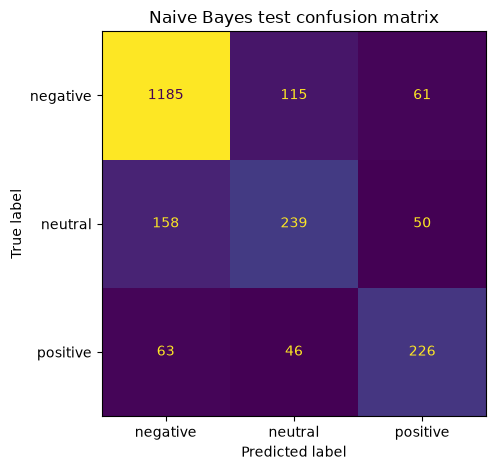
\includegraphics[width=.88\linewidth,height=5cm,keepaspectratio]{labs/visuals/07-notebook-reference.png}
\end{labvisual}
\begin{refoutput}
\begin{lstlisting}[style=utpterminal]
               model  accuracy  macro_precision  macro_recall  macro_f1
0  Majority baseline    0.6351           0.2117        0.3333    0.2589
1     Multinomial NB    0.7699           0.7036        0.6933    0.6978
\end{lstlisting}
\end{refoutput}

\textbf{What it means.} On the untouched test set Naive Bayes reaches about 77\,\% accuracy and 0.70 macro F1, against 63\,\% and 0.26 for the baseline. The confusion matrix shows the typical pattern: negative tweets are recognised well, while \emph{neutral} tweets are pulled towards \emph{negative}, because complaint vocabulary dominates the corpus.
\end{labanswer}

\begin{labquestion}{7}{Inspect subgroup performance and review errors}
Report per-class precision, recall and F1, then macro F1 per airline (\texttt{per\_airline\_f1.csv}). Finally take the four most confident mistakes for each true class, twelve deterministic errors, tag each with a simple category, and save \texttt{error\_analysis.csv}.
\end{labquestion}
\begin{labanswer}
\lstinputlisting[style=utppython,firstline=106,lastline=136]{all_experiments/lab07_airline_sentiment_worked.py}
\begin{refoutput}
\begin{lstlisting}[style=utpterminal]
          precision  recall     f1  support
negative      0.843   0.871  0.857     1361
neutral       0.598   0.535  0.564      447
positive      0.671   0.675  0.673      335
macro F1 by airline: Delta 0.659, American 0.662, United 0.675,
                     US Airways 0.714, Southwest 0.726, Virgin America 0.782 (63 tweets)
Saved: ['confusion_matrix.csv', 'confusion_matrix.png', 'error_analysis.csv', 'metrics.csv', 'per_airline_f1.csv', 'per_class_metrics.csv', 'split.csv', 'test_predictions.csv', 'validation_results.csv']
\end{lstlisting}
\end{refoutput}

\textbf{What it means.} Neutral is the hardest class, because it has few distinctive words and sits between the other two. The airline table is a diagnostic rather than a ranking: Virgin America's score rests on 63 tweets. Read the twelve sampled errors yourself. All twelve carry confidence above 0.999, which is why these scores cannot be treated as probabilities of being right.
\end{labanswer}

\begin{yourturn}
Add new cells at the end of the notebook. Choose settings on \emph{validation} data only, using the loop from Question~5 as a pattern, and keep the test set out of it.
\begin{enumerate}
  \item \textbf{Question a default.} Refit with \texttt{stop\_words=None}, keeping $\alpha=0.3$ and bigrams. What happens to validation macro F1, and why might it? Check whether \texttt{not}, \texttt{no} and \texttt{never} are in \texttt{sklearn.feature\_extraction.text.ENGLISH\_STOP\_WORDS}.
  \item \textbf{Try other settings.} Compare \texttt{min\_df=5}, $\alpha=0.1$, and \texttt{TfidfVectorizer} in place of \texttt{CountVectorizer}. Which help?
  \item \textbf{Look inside the model.} For each class, list the twelve terms with the highest log-probability relative to the other two classes, using the code below. Which class has words that look useful for future tweets, and which does not?
\end{enumerate}
\begin{lstlisting}[style=utppython]
names = np.array(features.get_feature_names_out())
log_prob = model.feature_log_prob_
for i, label in enumerate(model.classes_):
    others = [j for j in range(3) if j != i]
    odds = log_prob[i] - log_prob[others].mean(axis=0)
    print(label, list(names[np.argsort(-odds)[:12]]))
\end{lstlisting}
\end{yourturn}

\begin{expectedfindings}
\begin{enumerate}
  \item Validation macro F1 rises from 0.697 to 0.720, and the vocabulary reaches the 20,000 cap. All three words are on the stop list, along with \texttt{again}, so removing stop words was erasing negation and frequency words that carry sentiment. A default deserved testing.
  \item All three are slightly worse or clearly worse: \texttt{min\_df=5} gives 0.696, $\alpha=0.1$ gives 0.693, and TF-IDF with Multinomial Naive Bayes gives 0.633, because the model expects counts.
  \item Negative: \texttt{worst}, \texttt{ridiculous}, \texttt{hung}, \texttt{hold hours}, \texttt{unacceptable}, \texttt{terrible}, \texttt{rude}. Positive: \texttt{good work}, \texttt{guys rock}, \texttt{best airline}, \texttt{great flight}, \texttt{excellent}, \texttt{fantastic}. Those look reusable. Neutral: \texttt{journal}, \texttt{wall street}, \texttt{nantucket}, \texttt{license}, which are one-off news topics. That helps explain why neutral is the hardest class.
\end{enumerate}
\end{expectedfindings}

\begin{troubleshoot}
\begin{description}
  \item[Test metrics change between runs] Something is not seeded, or the test set is influencing a choice. Check \texttt{random\_state=42} in both splits.
  \item[Scores suspiciously high] Duplicates may have crept across the split. Confirm that \texttt{Tweets kept: 14285} appears before the split.
  \item[\texttt{ValueError} about empty vocabulary] You probably passed the wrong column. The vectoriser reads \texttt{model\_text}.
\end{description}
\end{troubleshoot}

\begin{verification}
\begin{itemize}
  \item Duplicates are removed before the split, leaving 14,285 tweets.
  \item The 70/15/15 split is stratified, fixed with seed~42, and saved to \texttt{split.csv}.
  \item The vectoriser is fitted on training tweets only, and the settings are chosen by validation macro F1.
  \item The test set is used once: Naive Bayes reaches about 0.70 macro F1 against 0.26 for the majority baseline.
  \item Per-class and per-airline results and the twelve reviewed errors are saved.
\end{itemize}
\end{verification}

\begin{labdeliverable}
\begin{itemize}
  \item Restart the kernel and run all cells without errors.
  \item Submit the executed notebook, including your \emph{Your turn} cells, and the generated \texttt{results/lab07/} folder.
  \item Add a short conclusion: explain why macro F1 is the headline metric, name the weakest class, and propose one stronger text representation without changing the evaluation protocol.
\end{itemize}
\end{labdeliverable}


\part{Local Search and Evolutionary Optimization}
\chapter{Local Search: When Only the Answer Counts}
\label{ch:localsearch}

\chapterguide%
  {Know the search loop of \chapref{ch:uninformed} and the heuristic idea of \chapref{ch:informed}, and be comfortable with random numbers in Python.}
  {explain when a problem needs a final answer rather than a route; run hill climbing by hand; say what a local maximum is and why random restarts and simulated annealing escape it; compute an annealing acceptance probability; and use beam search to keep several options alive.}

Until now the route was the answer. The robot needed the whole path to the charger, and we judged a search by what that path cost. Many problems are not like that. When you hand in a solved Sudoku, nobody asks what order you filled it in. A school timetable, a chip layout and the coefficients of a model are all judged only as finished products.

That changes what a search has to remember. If nobody needs the route, there is no reason to keep it. \term{Local search} keeps one candidate, or a few, and keeps improving them. It answers the fourth question from \chapref{ch:uninformed}: \emph{what if only the final answer counts?} This chapter has no lab of its own; it sets up the genetic algorithm of \chapref{ch:ga}, which Lab~8 practises. Every number below comes from \texttt{all\_experiments/demo\_local\_search.py}.

\section{The eight-queens puzzle}

Place eight queens on a chessboard so that no two attack each other. A queen attacks along its row, its column and both diagonals. Keep one queen in each column and each queen can sit on any of eight squares, which gives $8^8$, more than 16.7 million boards, and only 92 of them work.

We can run the search loop of \chapref{ch:uninformed} on this. The goal test is ``no attacks'' and a move shifts one queen. But breadth-first search has to hold a huge to-do list of boards just to reach an answer whose route nobody wants. So what if we keep just one board and keep making it better?

\section{Hill climbing}

Call fewer attacks higher ground, so that every better board is a step uphill. A board's \term{neighbours} are the boards we get by moving one queen up or down its own column. Eight queens with seven other squares each give $8\times7=56$ neighbours. \term{Hill climbing} moves to the best neighbour, then looks around and repeats, and it stops when no neighbour is better (\figref{fig:queens-board}).

\begin{analogy}
Picture yourself on a hillside in thick fog. You can only feel the ground right next to your feet, so you never plan ahead and you never look back. You take the steepest step up and repeat. When every step would go down, you stop and declare that you have reached the top. That may be a small foothill, with a far taller peak hidden across the valley.
\end{analogy}

\begin{utpfig}[One hill-climbing step on eight queens]{Left: a random board, written below it as the row of each column's queen, counting rows from zero at the top. Red lines join the 6 attacking pairs. Middle: hill climbing scores all 56 neighbours and moves to the best, which here has 3 attacking pairs. Right: the algorithm in plain words. Between moves it keeps only one board.}{fig:queens-board}
\begin{tikzpicture}[font=\small]
\def\q{0.38}
\foreach \r in {0,...,7}{\foreach \c in {0,...,7}{
  \pgfmathtruncatemacro{\odd}{mod(\r+\c,2)}
  \ifnum\odd=1
    \fill[UTPPaleBlue] (\q*\c,-\q*\r) rectangle ++(\q,-\q);
  \else
    \fill[white] (\q*\c,-\q*\r) rectangle ++(\q,-\q);
  \fi}}
\draw[draw=UTPBlue!55] (0,0) rectangle (8*\q,-8*\q);
\foreach \c/\r in {0/7,1/4,2/6,3/1,4/4,5/5,6/3,7/4}{
  \coordinate (Q\c) at ({\q*\c+\q/2},{-\q*\r-\q/2});
}
\foreach \a/\b in {1/4,1/7,2/4,4/5,4/7,6/7}{\draw[draw=UTPRed,thick] (Q\a)--(Q\b);}
\foreach \c in {0,...,7}{\node[circle,fill=UTPNavy,text=white,inner sep=0pt,minimum size=2.7mm,font=\tiny\bfseries] at (Q\c) {Q};}
\node[utplabel,anchor=north,align=center] at (4*\q,-8*\q-0.08) {7 4 6 1 4 5 3 4};
\begin{scope}[xshift=4.0cm,yshift=-1.5cm]
\draw[utparrow] (-0.35,0) -- (0.3,0);
\node[utpbox,minimum width=2.5cm,fill=UTPPaleOrange,draw=UTPOrange,align=center,font=\scriptsize\color{UTPNavy}] at (1.65,0) {score 56 neighbours\\take the fewest attacks};
\draw[utparrow] (3.0,0) -- (3.6,0);
\end{scope}
\node[anchor=west,align=left,text width=5.4cm,font=\scriptsize\color{UTPNavy}] at (7.75,-1.5) {%
  \textbf{Hill climbing}\\[2pt]
  \texttt{board} $\leftarrow$ a random board\\
  \textbf{repeat:}\\
  \quad score every neighbour of \texttt{board}\\
  \quad \textbf{if} the best is no better: \textbf{stop}\\
  \quad \texttt{board} $\leftarrow$ the best neighbour};
\end{tikzpicture}
\end{utpfig}

The memory saving is dramatic. Hill climbing holds at most 56 boards at any moment, and only one between moves. On one random board with 5 attacking pairs, the breadth-first loop expands 67,836 boards and its to-do list peaks at 456,001. Here is the whole of hill climbing in Python:

\lstinputlisting[style=utppython,firstline=39,lastline=49]{all_experiments/demo_local_search.py}

\begin{libnote}
You have met this idea already if you have trained a machine learning model. \term{Gradient descent} is hill climbing turned upside down: it walks downhill on the loss, the number that says how wrong the model is. ANFIS in \chapref{ch:fuzzy} used exactly this walk for its membership functions.
\end{libnote}

\section{Stuck on a local maximum}

The foggy hillside hides a weakness. Run hill climbing on the maze from \chapref{ch:uninformed} with higher ground meaning a smaller Manhattan guess, and the robot goes $(5,1)\to(4,1)\to(3,1)\to(2,1)$ and stops, with a guess of 8. Ahead of it is a wall, and every open neighbour guesses 9. No move looks better, so it quits long before the charger.

The same thing happens on the queens. A board where no single move helps is a \term{local maximum}. It can look fine from where you stand, and it still has attacking queens. How often does that happen? Over 1,000 random boards, hill climbing solves 150 and gets stuck on the other 850.

\section{Two ways to get unstuck}

\subsection{Random restarts}

The first fix is blunt. When you get stuck, throw the board away and climb again from a fresh random one. Keep doing that and you will eventually land on the right hillside, so \term{random-restart hill climbing} always solves the board in the end. It takes 7.3 climbs on average and looks at about 1,700 boards per puzzle solved.

\subsection{Simulated annealing}

Restarts throw away a whole board every time you are stuck. Is there a gentler way off a hilltop? What if the robot sometimes took a step downhill on purpose? It sounds like the dumbest idea in this book, and it works.

\begin{analogy}
The trick comes from metalworking and crystal growing. Melt a material and then cool it slowly. While it is hot its atoms move around freely, and as it cools they settle into a neat, low-energy crystal. Cool it too fast and the atoms freeze in a disordered jumble. That slow cooling is called \term{annealing}.
\end{analogy}

In 1983 Kirkpatrick, Gelatt and Vecchi, then at IBM, turned this into a search and used it to design computer chips. \term{Simulated annealing} picks one random move at each step. If the move is no worse, it always takes it. If the move is worse, it may still take it, with a chance that depends on how much worse the move is and on a \term{temperature} $T$ that falls a little at every step:
\[
P(\text{accept a move that adds } \Delta \text{ attacks}) \;=\; e^{-\Delta/T}.
\]

\figref{fig:annealing} shows what that formula does. At $T=1$ a move adding one attack gets through 37 times in 100, and a move adding three gets through about 5 times in 100. At $T=0.1$, one extra attack counts as heavily as ten did before, so it gets through only about 5 times in 100,000. While the search is hot it wanders freely; as it cools it behaves more and more like plain hill climbing.

\begin{utpfig}[Cooling makes bad moves rarer]{The chance of accepting a move that adds $\Delta$ attacks, as the temperature falls. Hot searches accept even bad moves often, which lets them walk off a local maximum. Cold searches almost never do. A move that is no worse ($\Delta\le0$) is always accepted.}{fig:annealing}
\begin{tikzpicture}
\begin{axis}[
  width=0.72\linewidth, height=5.0cm,
  xlabel={temperature $T$ (the search cools from right to left)}, ylabel={chance of accepting},
  xmin=0, xmax=1, ymin=0, ymax=0.42,
  ytick={0,0.1,0.2,0.3,0.4}, yticklabel style={/pgf/number format/fixed},
  axis lines=left, grid=major, grid style={draw=UTPPaleBlue},
  domain=0.03:1, samples=80, clip=false]
\addplot[draw=UTPBlue,very thick] {exp(-1/x)};
\addplot[draw=UTPTeal,very thick] {exp(-2/x)};
\addplot[draw=UTPOrange,very thick] {exp(-3/x)};
\node[font=\scriptsize\color{UTPBlue},anchor=south east] at (axis cs:0.98,0.37) {$\Delta=1$};
\node[font=\scriptsize\color{UTPTeal!70!black},anchor=south east] at (axis cs:0.98,0.14) {$\Delta=2$};
\node[font=\scriptsize\color{UTPOrange!85!black},anchor=south east] at (axis cs:0.98,0.05) {$\Delta=3$};
\end{axis}
\end{tikzpicture}
\end{utpfig}

\lstinputlisting[style=utppython,firstline=63,lastline=76]{all_experiments/demo_local_search.py}

Annealing has the restart built in. Instead of throwing the whole board away when stuck, it takes a small random step back, keeps the rest of its board, and climbs on from there. It solves 990 of the same 1,000 boards and looks at about 1,100 boards per puzzle solved, roughly 600 fewer than restarts.

\begin{pitfall}
Annealing has settings: a starting temperature, a cooling rate and a stopping temperature. Cool too quickly and it behaves like hill climbing and freezes on a local maximum. Cool too slowly and it wastes work. The demo starts at $T=1$, multiplies by 0.999 per step and stops below 0.01. Those values suit eight queens and are not universal.
\end{pitfall}

\section{Beam search: keep a few options}

Local search with one board has a blind spot. Suppose a phone keyboard wants the most likely short message that starts ``the flight''. It gives each possible next word a chance, and a message's chance is its words' chances multiplied together. \figref{fig:beam} uses a small table of chances written by hand.

Keeping one option means taking the single best word each time: ``is'' at 0.5, then ``late'' at 0.45, for a message scoring $0.5\times0.45=0.225$. But look at what got thrown away. ``Was'' scored only 0.4 at the first word, yet ``cancelled'' follows it with 0.8, for a message scoring $0.4\times0.8=0.32$. The best complete message started with a word that looked second best.

\begin{utpfig}[Beam search keeps the second-best word alive]{A hand-written table of next-word chances. With width 1 the search commits to ``is'' at the first word and can never recover. With width 2 it keeps both ``is'' and ``was'', scores every continuation, and finds the better message. Numbers on the right are whole-message chances.}{fig:beam}
\begin{tikzpicture}[font=\small,
  w/.style={utpcell,minimum width=1.55cm,minimum height=0.62cm,font=\scriptsize\bfseries\color{UTPNavy}},
  wk/.style={utpdone,minimum width=1.55cm,minimum height=0.62cm,font=\scriptsize\bfseries\color{UTPNavy}},
  wd/.style={utpdim,minimum width=1.55cm,minimum height=0.62cm,font=\scriptsize\color{UTPMuted}},
  lk/.style={semithick,draw=UTPTeal},
  pl/.style={utplabel,fill=white,inner sep=0.8pt}]
\node[w] (s) at (0,0) {the flight};
\node[wk] (a) at (3.0,1.0) {is};
\node[wk] (b) at (3.0,-0.2) {was};
\node[wd] (c) at (3.0,-1.3) {left};
\draw[lk] (s)--(a) node[midway,pl] {0.5};
\draw[lk] (s)--(b) node[midway,pl] {0.4};
\draw[draw=UTPMuted!50,semithick] (s)--(c) node[midway,pl] {0.1};
\node[wd] (a1) at (6.2,1.65) {late};
\node[wd] (a2) at (6.2,0.9) {full};
\node[wd] (a3) at (6.2,0.15) {here};
\draw[draw=UTPMuted!50,semithick] (a)--(a1) node[midway,pl] {0.45};
\draw[draw=UTPMuted!50,semithick] (a)--(a2) node[midway,pl] {0.35};
\draw[draw=UTPMuted!50,semithick] (a)--(a3) node[midway,pl] {0.20};
\node[wk,fill=UTPGreen!30] (b1) at (6.2,-0.6) {cancelled};
\node[wd] (b2) at (6.2,-1.3) {late};
\draw[lk,line width=1.2pt] (b)--(b1) node[midway,pl] {0.80};
\draw[draw=UTPMuted!50,semithick] (b)--(b2) node[midway,pl] {0.15};
\node[font=\scriptsize\color{UTPMuted},anchor=west] at (7.1,1.65) {0.225: width 1 stops here};
\node[font=\scriptsize\color{UTPMuted},anchor=west] at (7.1,0.9) {0.175};
\node[font=\scriptsize\color{UTPMuted},anchor=west] at (7.1,0.15) {0.100};
\node[font=\scriptsize\bfseries\color{UTPGreen!80!black},anchor=west] at (7.1,-0.6) {0.320: width 2 finds this};
\node[font=\scriptsize\color{UTPMuted},anchor=west] at (7.1,-1.3) {0.060};
\end{tikzpicture}
\end{utpfig}

\term{Beam search} fixes this by keeping the best $k$ options. At every step it grows every option it is holding, scores them all, keeps the best $k$ and drops the rest. The number $k$ is the \term{beam width}, and $k=1$ is hill climbing.

\lstinputlisting[style=utppython,firstline=136,lastline=144]{all_experiments/demo_local_search.py}

Real systems use exactly this idea. Machine translation systems choose each translated sentence by beam search, typically keeping a small handful of options at a time. A wider beam buys a slightly better sentence for more work, because every option you keep is one more to grow at every word. Once beam search drops an option, though, it never goes back, so it is not complete.

\section{The local search scorecard}

Here are the three board searches side by side, on the same 1,000 random boards. All three keep just one board between moves.

\begin{utptable}
\begin{tabularx}{\linewidth}{@{}>{\bfseries\leavevmode\color{UTPNavy}}m{0.24\linewidth}>{\centering\arraybackslash}m{0.17\linewidth}>{\centering\arraybackslash}m{0.20\linewidth}X@{}}
\toprule
\rowcolor{UTPPaleBlue!92}
\utpth{Search, eight queens} & \utpth{Boards solved} & \utpth{Looked at per solve} & \utpth{Note} \\
\midrule
Hill climbing & 150 of 1,000 & 1,555 & Stuck on the other 850 \\
Random restarts & 1,000 of 1,000 & 1,713 & 7.3 climbs on average \\
Simulated annealing & 990 of 1,000 & 1,107 & Can run out of temperature first \\
\bottomrule
\end{tabularx}
\end{utptable}

Read the third column with care. It divides all the work done by the boards actually solved, so plain hill climbing looks oddly close to the others. It only looks that way: hill climbing fails 85\,\% of the time, and one more climb on a failed board is exactly what random restarts adds.

\begin{keyidea}
When only the answer matters, keep one board and keep making it better. When it gets stuck, restart it, or take a worse step on purpose while it is still warm. When one option is too few, keep several.
\end{keyidea}

\begin{tryit}
Run \texttt{python all\_experiments/demo\_local\_search.py} from the course folder; it takes about a minute. Then, in a copy of the file, change \texttt{cooling=0.999} to \texttt{0.99}. The search now cools about ten times faster. Predict what happens to the number of boards solved and to the work per solve before you run it, and explain the result using \figref{fig:annealing}.

\emph{What to expect.} Boards solved falls from about 990 to about 490, because the search freezes before it has wandered enough. Work per solved board also falls, from about 1,100 to about 720, because a fast-cooling run gives up early. Speed has been bought with reliability.
\end{tryit}

\begin{chapterrecap}
\begin{itemize}
  \item Local search keeps candidates rather than routes, so it uses very little memory and suits problems judged only by the final answer.
  \item Hill climbing always takes the best neighbour and stops when none is better, which traps it on local maxima.
  \item Random restarts escape by starting over. Simulated annealing escapes by accepting worse moves with probability $e^{-\Delta/T}$ while it cools.
  \item Beam search keeps the best $k$ options at each step, because the option that looks second best now can turn out best later.
\end{itemize}
\end{chapterrecap}

\begin{quickcheck}
\begin{enumerate}
  \item Why does a Sudoku not need the path-cost piece of a search problem?
  \item How many neighbours does an eight-queens board have, and how does hill climbing use them?
  \item What is a local maximum on the eight-queens puzzle, in terms of attacking pairs?
  \item At temperature $T=0.5$, what is the chance of accepting a move that adds one attack?
  \item Explain why beam search with $k=1$ cannot find ``the flight was cancelled''.
\end{enumerate}
\end{quickcheck}

\chapter{Genetic Algorithms}
\label{ch:ga}

\chapterguide%
  {Know local search from \chapref{ch:localsearch}, be comfortable with NumPy arrays and random numbers, and know what a regression model and its RMSE are.}
  {name the parts of a genetic algorithm and what each contributes; encode a real-valued problem as a chromosome; implement tournament selection, blend crossover, Gaussian mutation and elitism; evaluate a stochastic optimiser over repeated seeds; and decide when an evolutionary method is justified against an exact one.}

Every search in \chapref{ch:localsearch} changes one candidate at a time: one queen on one board, one word added to one sentence. Each option only ever grows by itself. But two half-good solutions often have complementary strengths. What if they could combine?

Nature does this all the time, with two parents and a child that gets a bit of each. A \term{genetic algorithm} (GA) applies the same idea to candidate solutions. It improves a whole population through selection, recombination and random mutation, and it needs only a scoring function, not derivatives or convexity. Lab~8 tests a GA on a known one-dimensional function, then fits linear-regression coefficients. Ordinary least squares provides an exact, faster reference, so the aim is to evaluate a stochastic optimiser, not to claim it beats an exact method.

\section{Breeding boards: the idea on eight queens}

Start with the puzzle from \chapref{ch:localsearch}. A GA keeps a population of boards, say 50 random ones, and writes each board as eight digits, one per column, each saying which row that column's queen is in. Each board gets a \term{fitness}: the fewer attacking pairs, the fitter it is.

\begin{analogy}
Think of a raffle for the right to breed. Eight queens make 28 pairs, and a board gets one ticket for every pair that does \emph{not} attack. A board with 3 attacking pairs holds 25 tickets, and one with 10 holds 18. Draw two tickets to choose two parents. Fitter boards are likelier to be drawn, but even a poor board has a chance, which keeps variety in the population.
\end{analogy}

Two more steps make a child. In \term{crossover} we cut both parents at a random column and join the pieces. In \term{mutation}, now and then, one queen in the child jumps to a random row, which can create a row neither parent had (\figref{fig:breeding}).

\begin{utpfig}[Crossover and mutation on eight-queens boards]{A lucky pairing, chosen to show both operators. Each digit gives the row of one column's queen. Crossover cuts both parents after the same column and joins the left of one to the right of the other, and the child has only one attacking pair. Mutation then changes one digit to a row neither parent had in that column, and this board is solved.}{fig:breeding}
\begin{tikzpicture}[font=\small,
  ga/.style={cell,minimum width=0.58cm,minimum height=0.6cm,font=\small\bfseries\color{UTPNavy}},
  gb/.style={cellalt,minimum width=0.58cm,minimum height=0.6cm,font=\small\bfseries\color{UTPNavy}},
  gm/.style={cellbad,minimum width=0.58cm,minimum height=0.6cm,font=\small\bfseries\color{UTPRed}}]
\def\s{0.6}
\node[tagb,anchor=south west] at (-0.3,1.42) {parent 1: 5 attacking pairs};
\node[tagb,anchor=north west] at (-0.3,-0.22) {parent 2: 6 attacking pairs};
\foreach \d [count=\i from 0] in {1,4,6,3,1,6,2,5}{\node[ga] at (\s*\i,1.1) {\d};}
\foreach \d [count=\i from 0] in {1,4,2,2,0,7,4,2}{\node[gb] at (\s*\i,0.1) {\d};}
\draw[draw=UTPRed,dashed,thick] (\s*3+\s/2,1.42) -- (\s*3+\s/2,-0.22);
\node[utplabel,anchor=west,color=UTPRed] at (\s*3+\s/2+0.05,0.6) {cut};
\draw[utparrow] (4.7,0.6) -- (6.0,0.6) node[midway,above,utplabel] {crossover};
\begin{scope}[xshift=6.45cm]
\node[tagb,anchor=south] at (\s*3.5,0.92) {child: 1 attacking pair};
\foreach \d [count=\i from 0] in {1,4,6,3}{\node[ga] at (\s*\i,0.6) {\d};}
\foreach \d [count=\i from 4] in {0,7,4,2}{\node[gb] at (\s*\i,0.6) {\d};}
\end{scope}
\begin{scope}[xshift=6.45cm,yshift=-0.75cm]
\foreach \d [count=\i from 0] in {1,4,6,3}{\node[ga] at (\s*\i,0) {\d};}
\foreach \d [count=\i from 4] in {0,7}{\node[gb] at (\s*\i,0) {\d};}
\node[gm] at (\s*6,0) {5};
\node[gb] at (\s*7,0) {2};
\node[tagb,anchor=north] at (\s*3.5,-0.34) {after mutation: no attacks, solved};
\draw[utpptr,draw=UTPRed] (\s*6,0.98) -- (\s*6,0.34);
\node[utplabel,anchor=west,color=UTPRed] at (\s*7+0.42,0.68) {mutate $4\to5$};
\end{scope}
\end{tikzpicture}
\end{utpfig}

Repeat this to fill a new generation and let the children replace the population. Good pieces from two parents can then meet in one child, in a single step that a hill climber could not take. Here is that loop in Python, as the demo runs it:

\lstinputlisting[style=utppython,firstline=79,lastline=98]{all_experiments/demo_local_search.py}

Now the honest part. How well does it work on eight queens? In the demo, 171 of 200 runs find a solution within 1,000 generations, with a median of 328 generations among those that succeed. The work comes to about 27,000 boards per puzzle solved. Simulated annealing needed about 1,100.

\begin{keyidea}
Breeding boards sounds like the coolest idea in this book, and on eight queens the dumbest-sounding idea, annealing, does the job with less than a tenth of the work. When an idea sounds exciting, race it against a simple one first.
\end{keyidea}

GAs still earn their keep elsewhere. NASA used an evolutionary algorithm, a cousin of this one, to design an antenna for its Space Technology 5 mission. The result looks like a bent paper clip, nothing a human designer would draw, and it flew in space in 2006. Lab~8 tests the method on a problem where we know the exact answer, which is the fairest test of all.

\section{Vocabulary}

\begin{utptable}
\begin{tabularx}{\linewidth}{@{}>{\bfseries\leavevmode\color{UTPNavy}}m{0.14\linewidth}m{0.34\linewidth}m{0.21\linewidth}X@{}}
\toprule
\rowcolor{UTPPaleBlue!92}
\utpth{Term} & \utpth{Meaning} & \utpth{On eight queens} & \utpth{In Lab~8} \\
\midrule
Chromosome & One candidate solution, as a vector of genes & Eight digits, one per column & Five real numbers: intercept plus four coefficients \\
Gene & One component of a chromosome & One queen's row & One coefficient \\
Population & The set of chromosomes alive in one generation & 50 boards & 100 (or 40 in the sensitivity study) \\
Fitness & The score to be optimised & Pairs not attacking; higher is better & Training mean squared error; lower is better \\
Selection & Choosing parents, biased towards good fitness & Tickets (roulette wheel) & Tournament of three \\
Crossover & Combining two parents into children & Cut and join & Blend crossover \\
Mutation & Random perturbation of a child & One queen jumps & Gaussian noise on a random subset of genes \\
Elitism & Copying the best chromosomes unchanged into the next generation & None & The best 4 (or 2) survive \\
Generation & One pass of evaluate, select, cross, mutate, replace & Up to 1,000 passes & 160 passes per run \\
\bottomrule
\end{tabularx}
\end{utptable}

\section{One generation}

\figref{fig:ga-loop} combines selection pressure, recombination, mutation and preservation of the best candidates.

\begin{utpfig}[The genetic algorithm loop]{Selection favours better solutions, crossover recombines parents, mutation introduces variation, and elitism preserves the best candidates.}{fig:ga-loop}
\begin{tikzpicture}[
  b/.style={draw=UTPBlue,fill=UTPPaleBlue,rounded corners=2mm,minimum width=2.4cm,minimum height=0.9cm,align=center,font=\scriptsize\color{UTPNavy}},
  arr/.style={-{Stealth[length=2mm]},thick,draw=UTPTeal}
]
\node[b] (p) {Population};
\node[b,right=0.35cm of p] (fit) {Evaluate\\fitness};
\node[b,right=0.35cm of fit] (sel) {Select\\parents};
\node[b,right=0.35cm of sel] (cross) {Crossover};
\node[b,right=0.35cm of cross] (mut) {Mutation};
\node[b,below=1.0cm of sel,fill=UTPPaleTeal,draw=UTPGreen] (rep) {New generation\\= elites + children};
\draw[arr] (p)--(fit); \draw[arr] (fit)--(sel); \draw[arr] (sel)--(cross); \draw[arr] (cross)--(mut);
\draw[arr] (mut.south) |- (rep.east);
\draw[arr] (rep.west) -| (p.south);
\draw[arr,draw=UTPGreen,dashed] (fit.south) -- ++(0,-0.55) -| (rep.north) node[pos=0.25,below,xshift=-1cm,utplabel,color=UTPGreen] {best few copied unchanged (elitism)};
\end{tikzpicture}
\end{utpfig}

The lab uses the same loop for a single number $x$ and for a five-gene vector. The single-number version, which minimises $(x-3)^2$, shows all the moving parts in a few lines:

\lstinputlisting[style=utppython,firstline=28,lastline=39]{all_experiments/lab08_genetic_algorithm_regression_worked.py}

Vectorised operators avoid looping over individuals, so 160 generations of 100 chromosomes take a few hundredths of a second.

\section{Encoding: the chromosome is the answer}

For $\hat y=p_0+p_1x_1+\dots+p_4x_4$, encode each chromosome as five real coefficients. The GA searches the same space as least squares, which is what makes a direct comparison possible. Two details matter:

\begin{description}
  \item[Initialisation matters.] Charges are in thousands of dollars. Draw coefficients with mean~0 and standard deviation~5000, then shift the intercept towards the mean charge. Starting from $\mathcal N(0,1)$ would place the whole population far from useful values.
  \item[Standardise the inputs.] Age (18--64) and smoker status (0--1) have very different scales. Standardise all four predictors using training statistics so that a mutation step means roughly the same thing for each coefficient.
\end{description}

\begin{intuition}
The chromosome \emph{is} the candidate answer, read by the fitness function. Operators depend on the encoding: blend crossover suits real coefficients, cut-and-join suits eight-queens boards, and neither would make sense on a route that must visit every city exactly once.
\end{intuition}

\section{The operators}

\subsection{Fitness}

Fitness is training mean squared error. The lab evaluates it for the whole population in one matrix product:

\lstinputlisting[style=utppython,firstline=66,lastline=68]{all_experiments/lab08_genetic_algorithm_regression_worked.py}

Evaluating 100 five-gene chromosomes on 1,070 training rows produces a $100\times1{,}070$ prediction matrix, computed in one step rather than in a Python loop.

\subsection{Selection}

\term{Tournament selection} samples $k$ chromosomes and keeps the fittest, like picking the winner of a small heat; Lab~8 uses $k=3$. Unlike \term{roulette-wheel} selection (\figref{fig:roulette}), which is the raffle from eight queens, it does not depend on the scale of the fitness values and needs no conversion when lower is better. The tournament size sets the selection pressure. With $k=1$ there is no selection at all, and on Lab~8 the seed-to-seed spread jumps from $0.002$ to about 11.5.

\begin{utpfig}[Roulette-wheel selection]{Arc widths are proportional to fitness: B is selected four times as often as D. Tournament selection favours fitter candidates without depending on fitness scale.}{fig:roulette}
\begin{tikzpicture}[font=\small]
\node[utplabel,font=\small\bfseries\color{UTPNavy}] at (0,2.1) {Selection probabilities};
\def\rad{1.75}
\foreach \a/\b/\lbl/\col in {0/144/B/UTPBlue, 144/252/A/UTPTeal, 252/324/C/UTPOrange, 324/360/D/UTPRed}{
  \fill[\col!28,draw=\col,thick] (0,0) -- (\a:\rad) arc[start angle=\a,end angle=\b,radius=\rad] -- cycle;
  \pgfmathsetmacro{\mid}{(\a+\b)/2}
  \node[font=\small\bfseries\color{UTPNavy}] at (\mid:0.65*\rad) {\lbl};
}
\node[utplabel,anchor=north,align=center] at (0,-2.0)
  {Fitness $(B,A,C,D)=(4,3,2,1)$};
\begin{scope}[xshift=4.0cm,yshift=-0.4cm]
\def\L{7.2}
\node[utplabel,font=\small\bfseries\color{UTPNavy}] at (0.5*\L,2.5)
  {Cumulative probability};
\foreach \s/\e/\lbl/\col in {0/0.40/B/UTPBlue, 0.40/0.70/A/UTPTeal, 0.70/0.90/C/UTPOrange, 0.90/1.0/D/UTPRed}{
  \pgfmathsetmacro{\x}{\s*\L}
  \pgfmathsetmacro{\w}{(\e-\s)*\L}
  \fill[\col!28,draw=\col,thick] (\x,0) rectangle ++(\w,0.85);
  \node[font=\small\bfseries\color{UTPNavy}] at (\x+\w/2,0.42) {\lbl};
}
\foreach \v/\x in {0/0, 0.40/0.40, 0.70/0.70, 0.90/0.90, 1.0/1.0}{
  \pgfmathsetmacro{\xx}{\x*\L}
  \node[utplabel] at (\xx,-0.28) {\v};
}
\draw[-{Stealth[length=2.4mm]},line width=1.2pt,draw=UTPNavy] (0.54*\L,1.5) -- (0.54*\L,0.95);
\node[utplabel,anchor=south,color=UTPNavy] at (0.54*\L,1.55) {\texttt{rand} $=0.54\ \Rightarrow$ pick A};
\node[utplabel,anchor=north,align=center,text width=6.8cm] at (0.5*\L,-0.75)
  {The draw $0.54$ falls in A\textquotesingle s interval, $0.40$ to $0.70$.};
\end{scope}
\end{tikzpicture}
\end{utpfig}

\subsection{Crossover and mutation}

Cutting a list of real coefficients and joining the pieces would work poorly, because a good value of one gene is not tied to a position. \term{Blend crossover} forms $\alpha\,a+(1-\alpha)\,b$ from two parents instead. With $\alpha\in[0,1]$, children lie between them. The regression GA uses $\alpha\in[-0.1,1.1]$, which allows a child to land just beyond a parent (\figref{fig:crossover}). \term{Gaussian mutation} adds noise to a random 15\,\% of genes using per-gene step sizes. Without it the population can only contract: with the mutation rate set to zero, Lab~8's median test RMSE stays stuck at about 6,534 instead of reaching 5,829.

\begin{utpfig}[Crossover and mutation for real-valued genes]{Left: blend crossover places children between parents or slightly beyond them. Right: Gaussian mutation perturbs a child by a random step.}{fig:crossover}
\begin{tikzpicture}[font=\small]
\begin{scope}
\node[font=\bfseries\color{UTPNavy}] at (2.0,2.65) {Blend crossover};
\draw[-{Stealth[length=2mm]},draw=UTPMuted] (-0.2,0)--(4.4,0) node[right,font=\scriptsize] {$p_1$};
\draw[-{Stealth[length=2mm]},draw=UTPMuted] (0,-0.2)--(0,1.85) node[above,font=\scriptsize] {$p_2$};
\node[circle,fill=UTPBlue,inner sep=2.2pt,label={[utplabel,color=UTPBlue]above:parent $a$}] (P1) at (0.7,1.35) {};
\node[circle,fill=UTPTeal,inner sep=2.2pt,label={[utplabel,color=UTPTeal]below:parent $b$}] (P2) at (3.6,0.45) {};
\draw[draw=UTPMuted!60,dashed] (P1)--(P2);
\node[circle,fill=UTPOrange,inner sep=2.2pt] (Ch) at (1.86,1.0) {};
\node[utplabel,anchor=west,color=UTPOrange] at (2.0,1.28) {child, $\alpha=0.6$};
\node[utplabel,anchor=north,align=center,text width=4.8cm] at (2.0,-1.15)
  {$\alpha\in[-0.1,1.1]$ lets a child land just beyond a parent};
\end{scope}
\begin{scope}[xshift=6.6cm]
\node[font=\bfseries\color{UTPNavy}] at (2.2,2.65) {Gaussian mutation};
\draw[-{Stealth[length=2mm]},draw=UTPMuted] (-0.2,0)--(4.4,0) node[right,font=\scriptsize] {$p_1$};
\draw[-{Stealth[length=2mm]},draw=UTPMuted] (0,-0.2)--(0,1.85) node[above,font=\scriptsize] {$p_2$};
\node[circle,fill=UTPOrange,inner sep=2.2pt,label={[utplabel,color=UTPOrange]below:child}] (C) at (1.9,0.9) {};
\draw[draw=UTPOrange!35,fill=UTPOrange!10] (1.9,0.9) circle (0.75);
\node[circle,fill=UTPRed,inner sep=2.2pt,label={[utplabel,color=UTPRed]above right:mutated child}] (M) at (2.45,1.3) {};
\draw[utpptr,draw=UTPRed] (C)--(M);
\node[utplabel,anchor=north,align=center,text width=5.2cm] at (2.2,-1.15)
  {each gene moves by $\mathcal N(0,\sigma)$ with probability $0.15$; $\sigma$ is set per gene};
\end{scope}
\end{tikzpicture}
\end{utpfig}

\subsection{Elitism}

\term{Elitism} copies the best chromosomes unchanged into the next generation, so that selection or mutation cannot lose them. Think of an athletics squad that always keeps its current record holder. It costs a few population slots and means that the best fitness in the population can never get worse. Without elites, the best member of the population got worse in 54 of 159 generations on one Lab~8 run.

\begin{keyidea}
Selection favours good candidates, crossover recombines, mutation explores and elitism preserves. Tournament size~3, 15\,\% mutation and four elites are one workable balance, not universal settings.
\end{keyidea}

\section{Verifying before trusting}

Wrong fitness signs or mutation scales may not raise any error message: the code just runs and gives poor answers. So Lab~8 first minimises $f(x)=(x-3)^2$, whose answer we know, reaching about $10^{-5}$ from $x=3$ in 80 generations. Only then does it move on to regression, where least squares supplies a second check.

\section{Judging a stochastic optimiser}

A GA uses random numbers, so one seed shows only one outcome. Lab~8 reports results over ten seeds and compares them with an exact method.

\begin{utptable}
\begin{tabularx}{\linewidth}{@{}>{\bfseries\leavevmode\color{UTPNavy}}m{0.28\linewidth}>{\centering\arraybackslash}X>{\centering\arraybackslash}X>{\centering\arraybackslash}X@{}}
\toprule
\rowcolor{UTPPaleBlue!92}
\utpth{Method} & \utpth{Median test RMSE} & \utpth{SD across seeds} & \utpth{Median runtime} \\
\midrule
GA, population 100 & 5829.38 & 0.002 & 0.04 s \\
GA, population 40 & 5829.38 & 0.026 & 0.02 s \\
Ordinary least squares & 5829.38 & --- & $<$ 0.001 s \\
\bottomrule
\end{tabularx}
\end{utptable}

Three lessons follow:

\begin{description}
  \item[The GA approaches the optimum.] Runs agree within a few thousandths and match OLS performance, and the median coefficients match OLS to one decimal place.
  \item[It did not beat the optimum.] Least squares solves the same problem exactly and faster. Agreement verifies the GA; it shows no advantage over OLS.
  \item[Population size trades speed for spread.] Forty chromosomes halve the runtime with the same median, but increase seed-to-seed standard deviation by an order of magnitude. Judge that trade against the cost of a poor run.
\end{description}

\begin{pitfall}
Report the median and spread across independent seeds, not one run or the best run presented as typical. A lucky seed says nothing about the next one. On eight queens the median successful run took 328 generations, and 29 of the 200 runs did not finish at all.
\end{pitfall}

\section{When is a genetic algorithm the right tool?}

Least squares suits Lab~8's smooth, convex, unconstrained objective. Recall the bowl from \chapref{ch:fuzzy}: one lowest point and a formula that jumps straight there. Consider a GA when the problem is nothing like a bowl:

\begin{itemize}
  \item the objective is \textbf{non-differentiable} or only available as a black box (a simulation, a physical test rig);
  \item some variables are \textbf{discrete or mixed} (which features to include, which route to take, which schedule to run), so there is no gradient to follow;
  \item the objective is \textbf{multimodal}, with many local optima that trap gradient methods;
  \item the constraints are \textbf{awkward}: business rules, integer budgets, or feasibility checks that are easy to test and impossible to write as equations.
\end{itemize}

Integer coefficients, penalties on non-zero coefficients or a plateaued loss would invalidate ordinary least squares. A GA would need a revised fitness function and possibly new operators, and the deliverable asks you to identify one such change.

\begin{chapterrecap}
\begin{itemize}
  \item A GA evolves a population: fitter candidates are selected, recombined and mutated, and the best may be kept unchanged.
  \item The encoding decides the operators. Eight digits suit cut-and-join; real coefficients suit blending and Gaussian noise.
  \item Verify on a problem with a known answer, then report the median and spread over independent seeds.
  \item A GA that matches an exact method has been verified, not vindicated. Race it against something simple, and reach for it when the problem has no formula and no gradient.
\end{itemize}
\end{chapterrecap}

\begin{quickcheck}
\begin{enumerate}
  \item What is the chromosome in Lab~8, and how many genes does it have?
  \item Why does the lab standardise the predictors before running the GA, when least squares would give the same fit either way?
  \item What can happen to the best fitness in the population without elitism, and why?
  \item Blend crossover with $\alpha\in[0,1]$ can only produce children between the parents. What does that do to a population over many generations, and which two choices in the lab counteract it?
  \item Ten seeds gave test RMSE within $0.002$ of each other. Why is that a stronger statement than one run that hit the OLS value exactly?
  \item On eight queens, a board has 4 attacking pairs. How many raffle tickets does it hold?
\end{enumerate}
\end{quickcheck}

\begin{checkanswers}
\begin{enumerate}
  \item A vector of five real numbers: the intercept and the coefficients of age, BMI, children and smoker status.
  \item One mutation step size is used for every coefficient gene. With unstandardised inputs the same step would be huge for one coefficient and negligible for another; least squares is indifferent because it solves the problem exactly rather than searching it.
  \item It can get worse: the best chromosome might not be selected, or might be crossed or mutated away, which happened in 54 of 159 generations on one run. Elitism copies it forward unchanged. The lab's \emph{best-so-far} curve never rises in either case, because it records the best chromosome ever seen.
  \item The population contracts towards its own centre, because every child lies between two existing points. The lab counteracts this with $\alpha\in[-0.1,1.1]$ (children can land just beyond a parent) and with Gaussian mutation.
  \item Agreement across ten independent seeds shows the algorithm \emph{reliably} finds the optimum. One exact hit could be a lucky seed and says nothing about the next run.
  \item $28-4=24$ tickets, one for every pair of queens that does not attack.
\end{enumerate}
\end{checkanswers}

\labsection{8}{Genetic Algorithms: Regression and Reproducibility}{sec:lab08-ga}

\begin{labproject}{Fit a medical-cost regression model with a Genetic Algorithm}
\textbf{Read first.} Chapters~\ref{ch:localsearch} and~\ref{ch:ga}.\\
\textbf{Goal.} Verify a NumPy GA, evaluate it across ten seeds, and compare it with exact least squares.\\
\textbf{Scenario.} Test whether a real-valued GA can recover useful linear-regression coefficients, and compare its stochastic behaviour with an exact baseline.\\
\textbf{Data.} \texttt{all\_datasets/lab08-insurance.csv} (1,338 policies).\\
\textbf{Notebook.} \texttt{all\_experiments/lab08\_genetic\_algorithm\_regression\_worked.ipynb}.\\
\textbf{Hand in.} The executed notebook, the \texttt{results/lab08/} folder and a short conclusion, as listed in the checklist at the end of this sheet.
\end{labproject}

\begin{labmode}
\begin{enumerate}
  \item Activate your course environment and confirm that the data file is in \texttt{all\_datasets/}.
  \item Start Jupyter from \texttt{all\_experiments/}, open the notebook, and choose \textbf{Restart Kernel and Run All Cells}. Everything runs in a few seconds.
\end{enumerate}
\begin{lstlisting}[style=utpterminal]
cd all_experiments
jupyter lab
\end{lstlisting}
Prefer a plain script? From the course folder, \texttt{python all\_experiments/lab08\_genetic\_algorithm\_regression\_worked.py} runs the same code and writes the same evidence.
\end{labmode}

\courselabflow{Test scalar GA}{Encode weights}{Evolve seeds}{Compare OLS}


\labroutine

\begin{yourturn}
\textbf{Warm-up on paper.} Run one generation of a GA by hand, minimising $f(x)=(x-3)^2$, with the population $x=\{-4,\ 1,\ 5,\ 8\}$. Compute each fitness and keep one elite. Hold a tournament of two between $x=1$ and $x=8$, and another between $x=-4$ and $x=5$. Blend the two winners with $\alpha=0.5$. Is the child better than both parents here?

\emph{Answer.} Fitness: $49$, $4$, $4$, $25$. The elite is $x=1$ or $x=5$ (they tie). The tournaments are won by $x=1$ and $x=5$. The blended child is $0.5\times1+0.5\times5=3$, with fitness 0, the exact answer. Blending two points either side of the optimum is why crossover is so strong here, and why real problems are rarely this kind.
\end{yourturn}

\textbf{Setup.} Run the imports and path setup first, and keep this kernel state for the later questions. In the script version the first seven lines also set the working directory.
\lstinputlisting[style=utppython,firstline=1,lastline=7]{all_experiments/lab08_genetic_algorithm_regression_worked.py}
\lstinputlisting[style=utppython,firstline=8,lastline=23]{all_experiments/lab08_genetic_algorithm_regression_worked.py}

\begin{labquestion}{1}{Verify the evolutionary loop}
Before touching real data, minimise $f(x) = (x-3)^2$ with a small real-valued GA (tournament selection, blend crossover, Gaussian mutation, two elites) and confirm that the best solution approaches $x = 3$.
\end{labquestion}
\begin{labanswer}
\courselabtrace{One generation in the regression GA}{Evaluate}{Decode coefficients and calculate training MSE}{Reproduce}{Selection, crossover, mutation, then elites}{Repeat}{Track best fitness; test final weights only}

\lstinputlisting[style=utppython,firstline=25,lastline=45]{all_experiments/lab08_genetic_algorithm_regression_worked.py}
\begin{refoutput}
\begin{lstlisting}[style=utpterminal]
Best x = 2.999989   f(x) = 0.00000000
\end{lstlisting}
\end{refoutput}

\textbf{What it means.} The best individual lands about $10^{-5}$ from $x = 3$ after 80 generations. The loop (evaluate, keep elites, select by tournament, blend, mutate, replace) is the same loop the regression GA uses below, so a bug would show up here first.
\end{labanswer}

\begin{labquestion}{2}{Prepare the regression task}
Predict charges from age, BMI, number of children and smoker status (0/1). Split 80/20 with seed 42, standardise the predictors with training statistics only, and save the split.
\end{labquestion}
\begin{labanswer}
\lstinputlisting[style=utppython,firstline=47,lastline=57]{all_experiments/lab08_genetic_algorithm_regression_worked.py}
\begin{refoutput}
\begin{lstlisting}[style=utpterminal]
{'rows': 1338, 'train': 1070, 'test': 268, 'predictors': ['age', 'bmi', 'children', 'smoker']}
\end{lstlisting}
\end{refoutput}

\textbf{What it means.} 1,070 training and 268 test rows. Standardising the inputs puts all four coefficients on a comparable scale, which matters for a GA because one mutation step size is used for every coefficient gene.
\end{labanswer}

\textbf{Connect it to the chapter.} Every generation below goes once around this loop.
% Reused from chapters/10-genetic-algorithms.tex
\begin{labvisual}{Recall the chapter model}
\begin{labgraphic}
\begin{tikzpicture}[
  b/.style={draw=UTPBlue,fill=UTPPaleBlue,rounded corners=2mm,minimum width=2.4cm,minimum height=0.9cm,align=center,font=\scriptsize\color{UTPNavy}},
  arr/.style={-{Stealth[length=2mm]},thick,draw=UTPTeal}
]
\node[b] (p) {Population};
\node[b,right=0.35cm of p] (fit) {Evaluate\\fitness};
\node[b,right=0.35cm of fit] (sel) {Select\\parents};
\node[b,right=0.35cm of sel] (cross) {Crossover};
\node[b,right=0.35cm of cross] (mut) {Mutation};
\node[b,below=1.0cm of sel,fill=UTPPaleTeal,draw=UTPGreen] (rep) {New generation\\= elites + children};
\draw[arr] (p)--(fit); \draw[arr] (fit)--(sel); \draw[arr] (sel)--(cross); \draw[arr] (cross)--(mut);
\draw[arr] (mut.south) |- (rep.east);
\draw[arr] (rep.west) -| (p.south);
\draw[arr,draw=UTPGreen,dashed] (fit.south) -- ++(0,-0.55) -| (rep.north) node[pos=0.25,below,xshift=-1cm,utplabel,color=UTPGreen] {best few copied unchanged (elitism)};
\end{tikzpicture}
\end{labgraphic}\end{labvisual}


\begin{labquestion}{3}{Define the chromosome, fitness and operators}
A chromosome has five real-valued genes: the intercept and four coefficients. Fitness is the training mean squared error. Write \texttt{run\_ga} with tournament selection, blend crossover, Gaussian mutation and elitism, returning train RMSE, test RMSE, runtime and the best-so-far history. Run it once to check that it works.
\end{labquestion}
\begin{labanswer}
Keep the mapping from genes to the intercept and coefficients fixed, and inspect the prediction expression inside \texttt{run\_ga} before changing mutation:
\courselabtrace{Trace regression chromosomes and fitness}{1. Input / state}{X contains age, bmi, children and the smoker indicator; the scaler is fitted on training rows.}{2. Operation}{run\_ga searches coefficient vectors using training fitness; test errors are reported separately.}{3. Check}{Compare ten seeds with OLS on the identical X\_train and X\_test representation.}


\lstinputlisting[style=utppython,firstline=59,lastline=95]{all_experiments/lab08_genetic_algorithm_regression_worked.py}
\begin{refoutput}
\begin{lstlisting}[style=utpterminal]
seed 1: train RMSE 6113.1 | test RMSE 5829.4 | 0.04 s
Best chromosome [intercept, age, bmi, children, smoker]: [13346.1  3616.3  1978.4   519.2  9559.3]
\end{lstlisting}
\end{refoutput}

\textbf{What it means.} One run of 160 generations with a population of 100 takes a fraction of a second and already produces a coefficient vector with a large positive smoker effect, as expected. Each gene is a coefficient, so the GA searches the same space as least squares, only without gradients. A low training error is not by itself evidence of generalisation, so read the test RMSE across seeds next.
\end{labanswer}

\begin{labquestion}{4}{Run ten independent seeds}
Repeat the GA for seeds 1--10, save train RMSE, test RMSE and runtime per seed to \texttt{ga\_10\_runs.csv}, and summarise the spread across seeds.
\end{labquestion}
\begin{labanswer}
\lstinputlisting[style=utppython,firstline=97,lastline=105]{all_experiments/lab08_genetic_algorithm_regression_worked.py}
\begin{refoutput}
\begin{lstlisting}[style=utpterminal]
Median test RMSE 5829.38 | SD across seeds 0.0019
\end{lstlisting}
\end{refoutput}

\textbf{What it means.} All ten seeds converge to practically the same solution: the standard deviation of test RMSE across seeds is a few thousandths on a scale of thousands. This is the reproducibility evidence a single lucky run cannot provide.
\end{labanswer}

\begin{labquestion}{5}{Compare with least squares}
Fit ordinary least squares on the identical split and preprocessing, compare its test RMSE and coefficients with the GA, and plot the best-so-far training RMSE of five seeds against the OLS training RMSE.
\end{labquestion}
\begin{labanswer}
\lstinputlisting[style=utppython,firstline=107,lastline=121]{all_experiments/lab08_genetic_algorithm_regression_worked.py}
\begin{labvisual}{Reference plot from the supplied notebook}
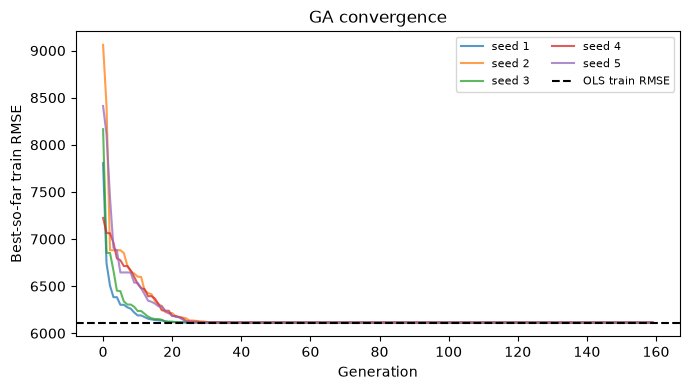
\includegraphics[width=.88\linewidth,height=5cm,keepaspectratio]{labs/visuals/08-notebook-reference.png}
\end{labvisual}
\begin{refoutput}
\begin{lstlisting}[style=utpterminal]
OLS test RMSE: 5829.38
OLS coefficients:    [3616.3 1978.4  519.2 9559.3]
Median GA coefficients: [3616.3 1978.4  519.2 9559.3]
\end{lstlisting}
\end{refoutput}

\textbf{What it means.} The GA's median test RMSE equals the OLS test RMSE to within rounding, and its coefficients match the OLS coefficients. Every seed drops onto the OLS line within a few dozen generations. The GA has \emph{found} the optimum; it has not \emph{beaten} it. For an unconstrained least-squares problem the closed-form solution is exact and far cheaper.
\end{labanswer}

\begin{labquestion}{6}{Run one sensitivity study}
Reduce the population from 100 to 40, repeat the ten seeds, and compare median test RMSE, its spread and runtime for both settings and OLS. Save \texttt{ga\_sensitivity\_pop40.csv} and \texttt{summary.csv}.
\end{labquestion}
\begin{labanswer}
\lstinputlisting[style=utppython,firstline=123,lastline=133]{all_experiments/lab08_genetic_algorithm_regression_worked.py}
\begin{refoutput}
\begin{lstlisting}[style=utpterminal]
       method  median_test_rmse  sd_test_rmse  median_runtime_s
0  GA pop=100         5829.3787        0.0019            0.0391
1   GA pop=40         5829.3819        0.0255            0.0176
2         OLS         5829.3785        0.0000               NaN
Saved: ['convergence.png', 'ga_10_runs.csv', 'ga_sensitivity_pop40.csv', 'split.csv', 'summary.csv']
\end{lstlisting}
\end{refoutput}

\textbf{What it means.} Forty chromosomes halve the runtime with the same median, and increase the seed-to-seed spread by more than ten times. On this easy problem both are fine. On a problem where a poor run is expensive, the spread is what you would be buying with those extra chromosomes.
\end{labanswer}

\begin{yourturn}
Add new cells at the end of the notebook. For every task, hold the split fixed, repeat over seeds 1--10, and report the median and standard deviation of test RMSE beside the OLS result. A helper saves typing:
\begin{lstlisting}[style=utppython]
def study(**settings):
    scores = [run_ga(seed, **settings)["test_rmse"] for seed in range(1, 11)]
    return round(np.median(scores), 2), round(np.std(scores, ddof=1), 4)
print(study(mutation_rate=0.0), study(mutation_rate=0.05), study(mutation_rate=0.5))
\end{lstlisting}
\begin{enumerate}
  \item \textbf{Mutation.} Try \texttt{mutation\_rate} 0, 0.05, 0.15 and 0.5, then \texttt{mutation\_scale} 0.01, 0.05, 0.25 and 1. What happens with no mutation at all, and why?
  \item \textbf{Budget.} Try \texttt{generations} 10, 20, 40 and 80. Where does extra budget stop paying?
  \item \textbf{Selection pressure.} Copy \texttt{run\_ga} and change the tournament size from 3 to 1, which means no selection at all. One result will look odd: the median test RMSE can fall \emph{below} the OLS value. Does that mean the GA has beaten least squares?
  \item \textbf{Write down one change} to the problem that would make a GA more appropriate than OLS, and what you would have to change in the fitness function or operators.
\end{enumerate}
\end{yourturn}

\begin{expectedfindings}
\begin{enumerate}
  \item With no mutation the median stays at about 6,534 with a spread of about 252: blending can only contract the population, so it collapses before reaching the optimum. Rates 0.05, 0.15 and 0.5 all reach about 5,829, with the tightest spread at 0.15. A scale of 0.01 is too timid (about 6,198); 0.05 and above reach the optimum.
  \item Median test RMSE is about 6,317, 5,952, 5,830 and 5,829.38. Almost nothing is gained after 80 generations, and the lab's 160 is a safe margin.
  \item With tournament size 1 the median is about 5,828.9 with a spread of about 11.5. It has not beaten anything. OLS minimises \emph{training} error, and it does so exactly. A run that has not converged can land closer to the test rows by chance, and the large spread is the giveaway. Its training RMSE is worse.
  \item Integer coefficients, a penalty on the number of non-zero coefficients, or a black-box cost all fit. Least squares no longer applies, so the fitness function changes, and integer genes would need new crossover and mutation.
\end{enumerate}
\end{expectedfindings}

\begin{troubleshoot}
\begin{description}
  \item[The GA never approaches OLS] Check the fitness sign (lower is better here) and that \texttt{X\_train} is the standardised matrix.
  \item[Results differ on every run] Pass the seed through to \texttt{np.random.default\_rng(seed)}. Do not use the global NumPy generator.
  \item[A shape error in \texttt{training\_mse}] Keep \texttt{individuals[:, [0]]} with the inner brackets, so that the intercept column broadcasts across the rows.
\end{description}
\end{troubleshoot}

\begin{verification}
\begin{itemize}
  \item The test GA finds $x\approx3$ for $f(x)=(x-3)^2$ before it is used on real data.
  \item The predictors are standardised with training statistics only (1,070 training and 268 test rows).
  \item Ten seeds are run, and \texttt{ga\_10\_runs.csv} records train RMSE, test RMSE and runtime for each.
  \item The GA's median test RMSE equals the least-squares test RMSE, and you can explain why it cannot beat it on training error.
  \item The population-40 sensitivity run is saved and its larger spread across seeds is explained.
\end{itemize}
\end{verification}

\begin{labdeliverable}
\begin{itemize}
  \item Restart the kernel and run all cells without errors.
  \item Submit the executed notebook, including your \emph{Your turn} cells, and the generated \texttt{results/lab08/} folder.
  \item Add a short conclusion: report the median and spread, explain why matching OLS is not beating it, and name one problem change that would make a GA more appropriate.
\end{itemize}
\end{labdeliverable}


\labsection{8}{Genetic Algorithms: Regression and Reproducibility}{sec:lab08-ga}

\begin{labproject}{Fit a medical-cost regression model with a Genetic Algorithm}
\textbf{Read first.} Chapters~\ref{ch:localsearch} and~\ref{ch:ga}.\\
\textbf{Goal.} Verify a NumPy GA, evaluate it across ten seeds, and compare it with exact least squares.\\
\textbf{Scenario.} Test whether a real-valued GA can recover useful linear-regression coefficients, and compare its stochastic behaviour with an exact baseline.\\
\textbf{Data.} \texttt{all\_datasets/lab08-insurance.csv} (1,338 policies).\\
\textbf{Notebook.} \texttt{all\_experiments/lab08\_genetic\_algorithm\_regression\_worked.ipynb}.\\
\textbf{Hand in.} The executed notebook, the \texttt{results/lab08/} folder and a short conclusion, as listed in the checklist at the end of this sheet.
\end{labproject}

\begin{labmode}
\begin{enumerate}
  \item Activate your course environment and confirm that the data file is in \texttt{all\_datasets/}.
  \item Start Jupyter from \texttt{all\_experiments/}, open the notebook, and choose \textbf{Restart Kernel and Run All Cells}. Everything runs in a few seconds.
\end{enumerate}
\begin{lstlisting}[style=utpterminal]
cd all_experiments
jupyter lab
\end{lstlisting}
Prefer a plain script? From the course folder, \texttt{python all\_experiments/lab08\_genetic\_algorithm\_regression\_worked.py} runs the same code and writes the same evidence.
\end{labmode}

\courselabflow{Test scalar GA}{Encode weights}{Evolve seeds}{Compare OLS}


\labroutine

\begin{yourturn}
\textbf{Warm-up on paper.} Run one generation of a GA by hand, minimising $f(x)=(x-3)^2$, with the population $x=\{-4,\ 1,\ 5,\ 8\}$. Compute each fitness and keep one elite. Hold a tournament of two between $x=1$ and $x=8$, and another between $x=-4$ and $x=5$. Blend the two winners with $\alpha=0.5$. Is the child better than both parents here?

\emph{Answer.} Fitness: $49$, $4$, $4$, $25$. The elite is $x=1$ or $x=5$ (they tie). The tournaments are won by $x=1$ and $x=5$. The blended child is $0.5\times1+0.5\times5=3$, with fitness 0, the exact answer. Blending two points either side of the optimum is why crossover is so strong here, and why real problems are rarely this kind.
\end{yourturn}

\textbf{Setup.} Run the imports and path setup first, and keep this kernel state for the later questions. In the script version the first seven lines also set the working directory.
\lstinputlisting[style=utppython,firstline=1,lastline=7]{all_experiments/lab08_genetic_algorithm_regression_worked.py}
\lstinputlisting[style=utppython,firstline=8,lastline=23]{all_experiments/lab08_genetic_algorithm_regression_worked.py}

\begin{labquestion}{1}{Verify the evolutionary loop}
Before touching real data, minimise $f(x) = (x-3)^2$ with a small real-valued GA (tournament selection, blend crossover, Gaussian mutation, two elites) and confirm that the best solution approaches $x = 3$.
\end{labquestion}
\begin{labanswer}
\courselabtrace{One generation in the regression GA}{Evaluate}{Decode coefficients and calculate training MSE}{Reproduce}{Selection, crossover, mutation, then elites}{Repeat}{Track best fitness; test final weights only}

\lstinputlisting[style=utppython,firstline=25,lastline=45]{all_experiments/lab08_genetic_algorithm_regression_worked.py}
\begin{refoutput}
\begin{lstlisting}[style=utpterminal]
Best x = 2.999989   f(x) = 0.00000000
\end{lstlisting}
\end{refoutput}

\textbf{What it means.} The best individual lands about $10^{-5}$ from $x = 3$ after 80 generations. The loop (evaluate, keep elites, select by tournament, blend, mutate, replace) is the same loop the regression GA uses below, so a bug would show up here first.
\end{labanswer}

\begin{labquestion}{2}{Prepare the regression task}
Predict charges from age, BMI, number of children and smoker status (0/1). Split 80/20 with seed 42, standardise the predictors with training statistics only, and save the split.
\end{labquestion}
\begin{labanswer}
\lstinputlisting[style=utppython,firstline=47,lastline=57]{all_experiments/lab08_genetic_algorithm_regression_worked.py}
\begin{refoutput}
\begin{lstlisting}[style=utpterminal]
{'rows': 1338, 'train': 1070, 'test': 268, 'predictors': ['age', 'bmi', 'children', 'smoker']}
\end{lstlisting}
\end{refoutput}

\textbf{What it means.} 1,070 training and 268 test rows. Standardising the inputs puts all four coefficients on a comparable scale, which matters for a GA because one mutation step size is used for every coefficient gene.
\end{labanswer}

\textbf{Connect it to the chapter.} Every generation below goes once around this loop.
% Reused from chapters/10-genetic-algorithms.tex
\begin{labvisual}{Recall the chapter model}
\begin{labgraphic}
\begin{tikzpicture}[
  b/.style={draw=UTPBlue,fill=UTPPaleBlue,rounded corners=2mm,minimum width=2.4cm,minimum height=0.9cm,align=center,font=\scriptsize\color{UTPNavy}},
  arr/.style={-{Stealth[length=2mm]},thick,draw=UTPTeal}
]
\node[b] (p) {Population};
\node[b,right=0.35cm of p] (fit) {Evaluate\\fitness};
\node[b,right=0.35cm of fit] (sel) {Select\\parents};
\node[b,right=0.35cm of sel] (cross) {Crossover};
\node[b,right=0.35cm of cross] (mut) {Mutation};
\node[b,below=1.0cm of sel,fill=UTPPaleTeal,draw=UTPGreen] (rep) {New generation\\= elites + children};
\draw[arr] (p)--(fit); \draw[arr] (fit)--(sel); \draw[arr] (sel)--(cross); \draw[arr] (cross)--(mut);
\draw[arr] (mut.south) |- (rep.east);
\draw[arr] (rep.west) -| (p.south);
\draw[arr,draw=UTPGreen,dashed] (fit.south) -- ++(0,-0.55) -| (rep.north) node[pos=0.25,below,xshift=-1cm,utplabel,color=UTPGreen] {best few copied unchanged (elitism)};
\end{tikzpicture}
\end{labgraphic}\end{labvisual}


\begin{labquestion}{3}{Define the chromosome, fitness and operators}
A chromosome has five real-valued genes: the intercept and four coefficients. Fitness is the training mean squared error. Write \texttt{run\_ga} with tournament selection, blend crossover, Gaussian mutation and elitism, returning train RMSE, test RMSE, runtime and the best-so-far history. Run it once to check that it works.
\end{labquestion}
\begin{labanswer}
Keep the mapping from genes to the intercept and coefficients fixed, and inspect the prediction expression inside \texttt{run\_ga} before changing mutation:
\courselabtrace{Trace regression chromosomes and fitness}{1. Input / state}{X contains age, bmi, children and the smoker indicator; the scaler is fitted on training rows.}{2. Operation}{run\_ga searches coefficient vectors using training fitness; test errors are reported separately.}{3. Check}{Compare ten seeds with OLS on the identical X\_train and X\_test representation.}


\lstinputlisting[style=utppython,firstline=59,lastline=95]{all_experiments/lab08_genetic_algorithm_regression_worked.py}
\begin{refoutput}
\begin{lstlisting}[style=utpterminal]
seed 1: train RMSE 6113.1 | test RMSE 5829.4 | 0.04 s
Best chromosome [intercept, age, bmi, children, smoker]: [13346.1  3616.3  1978.4   519.2  9559.3]
\end{lstlisting}
\end{refoutput}

\textbf{What it means.} One run of 160 generations with a population of 100 takes a fraction of a second and already produces a coefficient vector with a large positive smoker effect, as expected. Each gene is a coefficient, so the GA searches the same space as least squares, only without gradients. A low training error is not by itself evidence of generalisation, so read the test RMSE across seeds next.
\end{labanswer}

\begin{labquestion}{4}{Run ten independent seeds}
Repeat the GA for seeds 1--10, save train RMSE, test RMSE and runtime per seed to \texttt{ga\_10\_runs.csv}, and summarise the spread across seeds.
\end{labquestion}
\begin{labanswer}
\lstinputlisting[style=utppython,firstline=97,lastline=105]{all_experiments/lab08_genetic_algorithm_regression_worked.py}
\begin{refoutput}
\begin{lstlisting}[style=utpterminal]
Median test RMSE 5829.38 | SD across seeds 0.0019
\end{lstlisting}
\end{refoutput}

\textbf{What it means.} All ten seeds converge to practically the same solution: the standard deviation of test RMSE across seeds is a few thousandths on a scale of thousands. This is the reproducibility evidence a single lucky run cannot provide.
\end{labanswer}

\begin{labquestion}{5}{Compare with least squares}
Fit ordinary least squares on the identical split and preprocessing, compare its test RMSE and coefficients with the GA, and plot the best-so-far training RMSE of five seeds against the OLS training RMSE.
\end{labquestion}
\begin{labanswer}
\lstinputlisting[style=utppython,firstline=107,lastline=121]{all_experiments/lab08_genetic_algorithm_regression_worked.py}
\begin{labvisual}{Reference plot from the supplied notebook}
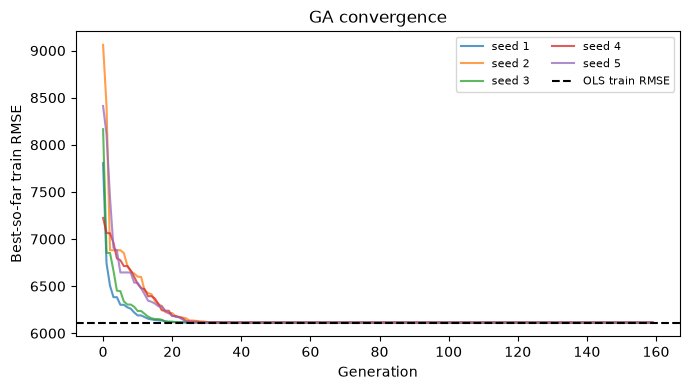
\includegraphics[width=.88\linewidth,height=5cm,keepaspectratio]{labs/visuals/08-notebook-reference.png}
\end{labvisual}
\begin{refoutput}
\begin{lstlisting}[style=utpterminal]
OLS test RMSE: 5829.38
OLS coefficients:    [3616.3 1978.4  519.2 9559.3]
Median GA coefficients: [3616.3 1978.4  519.2 9559.3]
\end{lstlisting}
\end{refoutput}

\textbf{What it means.} The GA's median test RMSE equals the OLS test RMSE to within rounding, and its coefficients match the OLS coefficients. Every seed drops onto the OLS line within a few dozen generations. The GA has \emph{found} the optimum; it has not \emph{beaten} it. For an unconstrained least-squares problem the closed-form solution is exact and far cheaper.
\end{labanswer}

\begin{labquestion}{6}{Run one sensitivity study}
Reduce the population from 100 to 40, repeat the ten seeds, and compare median test RMSE, its spread and runtime for both settings and OLS. Save \texttt{ga\_sensitivity\_pop40.csv} and \texttt{summary.csv}.
\end{labquestion}
\begin{labanswer}
\lstinputlisting[style=utppython,firstline=123,lastline=133]{all_experiments/lab08_genetic_algorithm_regression_worked.py}
\begin{refoutput}
\begin{lstlisting}[style=utpterminal]
       method  median_test_rmse  sd_test_rmse  median_runtime_s
0  GA pop=100         5829.3787        0.0019            0.0391
1   GA pop=40         5829.3819        0.0255            0.0176
2         OLS         5829.3785        0.0000               NaN
Saved: ['convergence.png', 'ga_10_runs.csv', 'ga_sensitivity_pop40.csv', 'split.csv', 'summary.csv']
\end{lstlisting}
\end{refoutput}

\textbf{What it means.} Forty chromosomes halve the runtime with the same median, and increase the seed-to-seed spread by more than ten times. On this easy problem both are fine. On a problem where a poor run is expensive, the spread is what you would be buying with those extra chromosomes.
\end{labanswer}

\begin{yourturn}
Add new cells at the end of the notebook. For every task, hold the split fixed, repeat over seeds 1--10, and report the median and standard deviation of test RMSE beside the OLS result. A helper saves typing:
\begin{lstlisting}[style=utppython]
def study(**settings):
    scores = [run_ga(seed, **settings)["test_rmse"] for seed in range(1, 11)]
    return round(np.median(scores), 2), round(np.std(scores, ddof=1), 4)
print(study(mutation_rate=0.0), study(mutation_rate=0.05), study(mutation_rate=0.5))
\end{lstlisting}
\begin{enumerate}
  \item \textbf{Mutation.} Try \texttt{mutation\_rate} 0, 0.05, 0.15 and 0.5, then \texttt{mutation\_scale} 0.01, 0.05, 0.25 and 1. What happens with no mutation at all, and why?
  \item \textbf{Budget.} Try \texttt{generations} 10, 20, 40 and 80. Where does extra budget stop paying?
  \item \textbf{Selection pressure.} Copy \texttt{run\_ga} and change the tournament size from 3 to 1, which means no selection at all. One result will look odd: the median test RMSE can fall \emph{below} the OLS value. Does that mean the GA has beaten least squares?
  \item \textbf{Write down one change} to the problem that would make a GA more appropriate than OLS, and what you would have to change in the fitness function or operators.
\end{enumerate}
\end{yourturn}

\begin{expectedfindings}
\begin{enumerate}
  \item With no mutation the median stays at about 6,534 with a spread of about 252: blending can only contract the population, so it collapses before reaching the optimum. Rates 0.05, 0.15 and 0.5 all reach about 5,829, with the tightest spread at 0.15. A scale of 0.01 is too timid (about 6,198); 0.05 and above reach the optimum.
  \item Median test RMSE is about 6,317, 5,952, 5,830 and 5,829.38. Almost nothing is gained after 80 generations, and the lab's 160 is a safe margin.
  \item With tournament size 1 the median is about 5,828.9 with a spread of about 11.5. It has not beaten anything. OLS minimises \emph{training} error, and it does so exactly. A run that has not converged can land closer to the test rows by chance, and the large spread is the giveaway. Its training RMSE is worse.
  \item Integer coefficients, a penalty on the number of non-zero coefficients, or a black-box cost all fit. Least squares no longer applies, so the fitness function changes, and integer genes would need new crossover and mutation.
\end{enumerate}
\end{expectedfindings}

\begin{troubleshoot}
\begin{description}
  \item[The GA never approaches OLS] Check the fitness sign (lower is better here) and that \texttt{X\_train} is the standardised matrix.
  \item[Results differ on every run] Pass the seed through to \texttt{np.random.default\_rng(seed)}. Do not use the global NumPy generator.
  \item[A shape error in \texttt{training\_mse}] Keep \texttt{individuals[:, [0]]} with the inner brackets, so that the intercept column broadcasts across the rows.
\end{description}
\end{troubleshoot}

\begin{verification}
\begin{itemize}
  \item The test GA finds $x\approx3$ for $f(x)=(x-3)^2$ before it is used on real data.
  \item The predictors are standardised with training statistics only (1,070 training and 268 test rows).
  \item Ten seeds are run, and \texttt{ga\_10\_runs.csv} records train RMSE, test RMSE and runtime for each.
  \item The GA's median test RMSE equals the least-squares test RMSE, and you can explain why it cannot beat it on training error.
  \item The population-40 sensitivity run is saved and its larger spread across seeds is explained.
\end{itemize}
\end{verification}

\begin{labdeliverable}
\begin{itemize}
  \item Restart the kernel and run all cells without errors.
  \item Submit the executed notebook, including your \emph{Your turn} cells, and the generated \texttt{results/lab08/} folder.
  \item Add a short conclusion: report the median and spread, explain why matching OLS is not beating it, and name one problem change that would make a GA more appropriate.
\end{itemize}
\end{labdeliverable}


\part{Adversarial Search}
\chapter{Adversarial Search: When Someone Fights Back}
\label{ch:games}

\chapterguide%
  {Know the search loop and DFS from \chapref{ch:uninformed}, and the idea of a heuristic from \chapref{ch:informed}.}
  {draw a game tree and pass scores up it by minimax; explain why a program must assume its opponent's best reply; say what alpha-beta pruning saves; explain what an evaluation function trades away; describe the four steps of Monte Carlo Tree Search; and place every search in this book on one cheat sheet.}

So far the robot has played alone. A maze wall does not move to block you, so once a route is found you can simply drive it. Now the robot plays noughts and crosses against a person, and the person is trying to win. This is the last of the five questions from \chapref{ch:uninformed}: \emph{what if someone fights back?}

It is still a search, with one twist: every other pick belongs to your opponent. A search with an opponent is called \term{adversarial search}. It is the idea behind the chess and Go results that opened \chapref{ch:uninformed}. This chapter has no lab, and every number in it is printed by \texttt{all\_experiments/demo\_game\_search.py}, which needs no dataset and finishes in about a second.

\section{Playing out every future}

The robot plays X and its opponent plays O. When a game ends, it gets a score: $+1$ if X wins, $-1$ if O wins, and $0$ for a draw. X wants the score as high as possible, so we call X the \term{Max} player. O wants it as low as possible, so O is the \term{Min} player.

Here is a game halfway through, with X to move and three squares empty: top left, top right and centre (\figref{fig:game-tree}). To choose, the robot plays out every possible future. That picture is a \term{game tree}: a search tree whose levels take turns.

\newcommand{\tttboard}[3]{%
  \begin{scope}[shift={(#1)},scale=0.27,transform shape]
    \draw[draw=UTPBlue!70,thick,fill=#3] (0,0) rectangle (3,-3);
    \draw[draw=UTPBlue!70] (1,0)--(1,-3) (2,0)--(2,-3) (0,-1)--(3,-1) (0,-2)--(3,-2);
    \foreach \sq [count=\k from 0] in {#2}{
      \pgfmathtruncatemacro{\cc}{mod(\k,3)}
      \pgfmathtruncatemacro{\rr}{int(\k/3)}
      \node[font=\Huge\bfseries\color{UTPNavy}] at (\cc+0.5,-\rr-0.5) {\sq};
    }
  \end{scope}%
}

\begin{utpfig}[The game tree from a halfway board]{Every future from the halfway board. Levels alternate: X moves, then O, then X. Scores on the leaves are for X. Passing them up, O takes the smallest and X the largest. Only the top-right move is worth $+1$, because it makes two lines X can finish and O can block only one.}{fig:game-tree}
\begin{tikzpicture}[font=\small,
  val/.style={circle,inner sep=0.7pt,minimum size=4.6mm,font=\scriptsize\bfseries\color{white}},
  vwin/.style={val,fill=UTPGreen},
  vdraw/.style={val,fill=UTPMuted},
  tline/.style={semithick,draw=UTPTeal!70},
  lvl/.style={utplabel,anchor=east,font=\scriptsize\bfseries\color{UTPNavy},align=right}]
% root
\tttboard{5.6,0}{{},X,{},O,{},X,X,O,O}{white}
\node[vwin] at (6.72,-0.42) {+1};
% X moves
\tttboard{1.0,-2.0}{X,X,{},O,{},X,X,O,O}{white}
\tttboard{5.6,-2.0}{{},X,X,O,{},X,X,O,O}{UTPPaleTeal}
\tttboard{10.2,-2.0}{{},X,{},O,X,X,X,O,O}{white}
\node[vdraw] at (2.12,-2.42) {0};
\node[vwin] at (6.72,-2.42) {+1};
\node[vdraw] at (11.32,-2.42) {0};
\node[utplabel,anchor=north] at (1.405,-2.84) {top left};
\node[utplabel,anchor=north] at (6.005,-2.84) {top right};
\node[utplabel,anchor=north] at (10.605,-2.84) {centre};
\draw[tline] (6.005,-0.82) -- (1.405,-2.0);
\draw[tline,line width=1.5pt,draw=UTPGreen] (6.005,-0.82) -- (6.005,-2.0);
\draw[tline] (6.005,-0.82) -- (10.605,-2.0);
% O replies
\tttboard{0,-4.15}{X,X,O,O,{},X,X,O,O}{white}
\tttboard{1.85,-4.15}{X,X,{},O,O,X,X,O,O}{white}
\node[vdraw] at (1.12,-4.45) {0};
\node[vwin] at (2.97,-4.45) {+1};
\tttboard{4.7,-4.15}{O,X,X,O,{},X,X,O,O}{white}
\tttboard{6.55,-4.15}{{},X,X,O,O,X,X,O,O}{white}
\node[vwin] at (5.82,-4.45) {+1};
\node[vwin] at (7.67,-4.45) {+1};
\tttboard{9.3,-4.15}{O,X,{},O,X,X,X,O,O}{white}
\tttboard{11.15,-4.15}{{},X,O,O,X,X,X,O,O}{white}
\node[vwin] at (10.42,-4.45) {+1};
\node[vdraw] at (12.27,-4.45) {0};
\foreach \a/\b in {1.405/0.405,1.405/2.255,6.005/5.105,6.005/6.955,10.605/9.705,10.605/11.555}{
  \draw[tline] (\a,-3.14) -- (\b,-4.15);
}
% X's last move: outcomes
\foreach \x/\t in {0.405/draw,2.255/X wins,5.105/X wins,6.955/X wins,9.705/X wins,11.555/draw}{
  \node[utplabel,anchor=north] at (\x,-4.98) {\t};
}
\node[lvl] at (-0.15,-0.4) {X (Max)\\takes the largest};
\node[lvl] at (-0.15,-2.4) {O (Min)\\takes the smallest};
\node[lvl] at (-0.15,-4.55) {X's last move\\is forced};
\end{tikzpicture}
\end{utpfig}

Now the tempting mistake. There is a $+1$ under the top-left move, so why not play it? Because a maze wall is not trying to stop you, and O is. If X takes the top left, O simply blocks at the top right and the game is drawn. The $+1$ only exists if O makes a mistake, and a robot cannot plan on mistakes. It has to assume O makes its best reply.

\section{Minimax}

So pass the scores up the tree. On O's level, O picks the reply that is worst for X, the smallest number. Under the top-left move O picks the 0. Under the centre, the same. But under the top-right move \emph{both} of O's replies lose, because X now has two lines to finish and O can block only one. On X's level, X takes the largest number, so X plays the top right and wins on its next move.

That is \term{minimax}: score every move by what happens after your opponent's best reply. In code, the passing up happens by itself through recursion.

\lstinputlisting[style=utppython,firstline=53,lastline=60]{all_experiments/demo_game_search.py}

Like DFS, this plays one line all the way to the end of the game before backing up to try the next, so it needs little memory: only the moves along the game it is currently imagining. And how good is the robot? Against an opponent moving at random, over 2,000 games it wins 1,746, draws 254 and loses none. When two minimax robots play each other the game is always drawn. From the empty board, minimax visits 549,946 positions and returns 0, which proves that with perfect play noughts and crosses is a draw.

\begin{analogy}
A careful chess player thinks ``if I do this, the best they can do is that, and then the best I can do is this''. Minimax is that sentence as an algorithm. Hoping your opponent will blunder is the beginner's version, and it is the error the top-left move in \figref{fig:game-tree} tempts you into.
\end{analogy}

\subsection{Alpha-beta: skipping futures that cannot matter}

Minimax looks at everything, and much of that is wasted. Suppose you have already found a move worth $+1$. While examining another move you discover that the opponent has a reply worth $-1$. You do not need to look at that opponent's other replies, because you already know you will not choose this move. \term{Alpha-beta pruning} tracks those two bounds and stops examining a move as soon as it cannot change the answer. The result is the same, and the work is far less: on the empty board 18,297 positions instead of 549,946, or 3.3\,\% of the work.

\section{When the tree is too big: guess and stop}

Chess is far bigger. In 1950 Claude Shannon, the father of information theory, estimated that a chess program would face about $10^{120}$ possible games. No computer could ever play them all out. So a chess program looks a few moves ahead, stops, and gives each board a score with a guess. That guess is an \term{evaluation function}, a heuristic for games. For chess the simplest guess adds up piece values: pawn 1, knight or bishop 3, rook 5, queen 9.

What does trusting a guess cost? Test it on our small game. A second robot gets a simple guess, the lines X could still finish minus the lines O could still finish, and looks only two moves ahead. It looks at about 142 positions per game, whereas full search visits 549,945 positions for its opening move alone. Over 200 games the full-search robot wins 34, draws 166 and loses none. The guess is far cheaper, and it costs games.

\begin{pitfall}
A robot that stops early is only as smart as its guess, exactly as A$^\star$ with a bad heuristic can only do so much. A good evaluation function took chess programmers decades to develop, and building one requires knowing the game.
\end{pitfall}

\begin{libnote}
Deep Blue beat Garry Kasparov in 1997 by doing exactly this: a fast version of minimax with pruning, a rich evaluation function, and special hardware examining around 200 million positions a second. Its strength came largely from raw search rather than from human-style understanding of chess, a point that Rich Sutton draws out in his 2019 essay \emph{The Bitter Lesson}.
\end{libnote}

\section{Monte Carlo Tree Search}

Go is much harder than chess. A chess player has about 35 moves to choose from each turn, while a Go player has about 250, and it is notoriously difficult to score a Go board by hand. So how do you search a tree that wide when you cannot even write an evaluation function?

Play lots of random games and count who wins. Judging a position by averaging random games is called a \term{Monte Carlo} method. On our halfway board, play 100 games to the end after each of X's three moves, with both sides moving at random. After the top right, X wins all 100. After the top left it wins 57, and after the centre 49. Those last two are really draws, and they score well only because random opponents make mistakes, but the votes still point at the right move with no evaluation function at all.

Spending the same number of games on every move is wasteful, though, and with 250 moves each turn it adds up quickly. \term{Monte Carlo Tree Search} (MCTS) spends its games more wisely by growing a tree as it plays (\figref{fig:mcts}).

\begin{utpfig}[The four steps of Monte Carlo Tree Search]{One game of MCTS. Walk down the tree, mostly towards moves that have won so far; add one new move; play a random game from there; and pass the result back up. After many games, play the move that was visited most.}{fig:mcts}
\begin{tikzpicture}[font=\small,
  n/.style={circle,draw=UTPBlue,fill=UTPPaleBlue,minimum size=5.4mm,inner sep=0pt},
  hot/.style={n,draw=UTPOrange,fill=UTPPaleOrange,line width=1pt},
  new/.style={n,draw=UTPGreen,fill=UTPPaleTeal,line width=1pt},
  l/.style={semithick,draw=UTPMuted!70},
  lh/.style={line width=1.3pt,draw=UTPOrange},
  ttl/.style={font=\scriptsize\bfseries\color{UTPNavy},align=center}]
\newcommand{\basetree}[1]{%
  \node[#1] (a) at (0,0) {};
  \node[n] (b) at (-0.65,-0.85) {};
  \node[n] (c) at (0.65,-0.85) {};
  \node[n] (d) at (0.15,-1.7) {};
  \draw[l] (a)--(b); \draw[l] (a)--(c); \draw[l] (c)--(d);}
\begin{scope}
\node[ttl] at (0,0.62) {1. Selection\\walk down};
\basetree{hot}
\node[hot] at (0.65,-0.85) {};
\node[hot] at (0.15,-1.7) {};
\draw[lh] (0,-0.27)--(0.5,-0.63); \draw[lh] (0.55,-1.09)--(0.27,-1.47);
\end{scope}
\begin{scope}[xshift=3.65cm]
\node[ttl] at (0,0.62) {2. Expansion\\add one move};
\basetree{n}
\node[new] (e) at (-0.25,-2.55) {};
\draw[l] (d)--(e);
\end{scope}
\begin{scope}[xshift=7.3cm]
\node[ttl] at (0,0.62) {3. Simulation\\a random game};
\basetree{n}
\node[new] (e) at (-0.25,-2.55) {};
\draw[l] (d)--(e);
\draw[draw=UTPOrange,thick,decorate,decoration={snake,amplitude=1.1pt,segment length=5pt}] (e.south) -- ++(0.1,-0.72);
\node[font=\scriptsize\bfseries\color{UTPOrange!85!black},anchor=west] at (0,-3.2) {X wins};
\end{scope}
\begin{scope}[xshift=10.95cm]
\node[ttl] at (0,0.62) {4. Backup\\pass it back up};
\basetree{n}
\node[new] (e) at (-0.25,-2.55) {};
\draw[l] (d)--(e);
\draw[-{Stealth[length=1.8mm]},draw=UTPGreen,thick] (-0.05,-2.3)--(0.08,-1.97);
\draw[-{Stealth[length=1.8mm]},draw=UTPGreen,thick] (0.28,-1.47)--(0.53,-1.09);
\draw[-{Stealth[length=1.8mm]},draw=UTPGreen,thick] (0.5,-0.63)--(0.13,-0.25);
\node[font=\scriptsize\color{UTPGreen!80!black},anchor=west] at (0.55,-1.65) {+1 win};
\end{scope}
\end{tikzpicture}
\end{utpfig}

Each game starts at the top and walks down. Mostly it heads for the moves that have won the most so far for whoever's turn it is, which is called \term{exploitation}. On the opponent's turns that means the opponent's best replies, so the more it plays, the less it counts on mistakes. Now and then it tries a move it has barely tried, which is called \term{exploration}. When the walk reaches a move never tried, MCTS adds it to the tree, plays one random game from there, and adds the result to every move on the way back up.

\begin{analogy}
Think of choosing a restaurant in a new town. You mostly return to the places that have been good, but you try somewhere new now and then in case it is better. Too much of the first and you may never find the best place. Too much of the second and you keep eating badly.
\end{analogy}

On our halfway board, 300 games of MCTS give the top right 284 visits and the other two moves 8 each, instead of 100 each as before. MCTS then plays the move it visited most.

\begin{libnote}
AlphaGo beat Lee Sedol four games to one in 2016 using this kind of search, steered by neural networks that had learned where to look: a policy network suggested promising moves and a value network guessed who was winning. It was still a search. Sutton's essay argues that search and learning are the two methods that keep getting better the more computing power you give them.
\end{libnote}

\section{One loop, one cheat sheet}

These searches began as separate names with no lines between them. Here is the sheet that holds them all. Each one fills the to-do list and chooses from it in its own way, and in every case the question is the same: what do we look at next?

\begin{utptable}
\begin{tabularx}{\linewidth}{@{}>{\bfseries\leavevmode\color{UTPNavy}}m{0.21\linewidth}m{0.33\linewidth}XX@{}}
\toprule
\rowcolor{UTPPaleBlue!92}
\utpth{Search} & \utpth{What it looks at next} & \utpth{Strength} & \utpth{Weakness} \\
\midrule
BFS & Oldest on the list & Fewest steps, guaranteed & Explores nearly everything \\
DFS & Newest on the list & Can be quick, little memory & Route may be poor; order dependent \\
Bidirectional & Oldest, from both ends & Skips the big outer rings & Needs one known goal \\
UCS (Dijkstra) & Least cost so far, $g$ & Cheapest route, guaranteed & Blind to direction \\
Greedy best-first & Smallest guess, $h$ & Very little work & Route may be poor \\
A$^\star$ & Smallest $g+h$ & Cheapest route with far less work & Needs a guess that never overestimates \\
Hill climbing & The best neighbour & One board in memory & Stuck on local maxima \\
Simulated annealing & A random neighbour, maybe worse & Escapes local maxima & Depends on the cooling schedule \\
Beam search & The best $k$ options & Keeps options open & Never returns to what it dropped \\
Genetic algorithm & Children of fit parents & Combines good parts & Often more work than simpler methods \\
Minimax & Every reply, assuming the best one & Best play against a perfect opponent & Tree too large for big games \\
Evaluation function & The tree only so deep, then a guess & Scales to chess & Only as good as the guess \\
MCTS & Moves that keep winning, plus a few new & Needs no handwritten guess & Random games can mislead \\
\bottomrule
\end{tabularx}
\end{utptable}

\begin{tryit}
Run \texttt{python all\_experiments/demo\_game\_search.py} from the course folder and find each number from this chapter. Then choose a different halfway board by editing \texttt{HALFWAY}, keeping X to move, and draw its game tree by hand before running the code. Do your minimax values match? Remove the final \texttt{assert} first, because it checks the book's board.
\end{tryit}

\begin{chapterrecap}
\begin{itemize}
  \item With an opponent, a found route is not enough, because the opponent gets to move too. Assume the best reply.
  \item Minimax passes scores up the game tree, taking the smallest on the opponent's level and the largest on yours. Alpha-beta skips moves that cannot change the answer.
  \item When the tree is too large, stop early and trust an evaluation function. The robot is then only as good as its guess.
  \item MCTS needs no guess at all: it lets random games vote and spends more of them on what keeps winning.
  \item Every search in this book is one loop with its own answer to one question: what do we look at next?
\end{itemize}
\end{chapterrecap}

\begin{quickcheck}
\begin{enumerate}
  \item In \figref{fig:game-tree}, why is the top-left move worth 0 even though a $+1$ sits below it?
  \item What does alpha-beta pruning change about minimax's answer, and what does it change about its work?
  \item Which earlier idea in this book is an evaluation function closest to?
  \item Why does flat Monte Carlo rate the centre move at 49 wins in 100 when minimax says it only draws?
  \item In MCTS, what is the difference between exploitation and exploration?
\end{enumerate}
\end{quickcheck}


\end{document}
